\documentclass[a4paper,12pt,oneside,openany,article]{memoir} %,draft twoside

\usepackage[utf8]{inputenc}
\usepackage[T2A,T1]{fontenc}
\usepackage[russian]{babel}
\usepackage{graphicx}
\graphicspath{ {media/} }
\usepackage{amsmath}
\usepackage{amssymb}
\usepackage{geometry}
\usepackage{booktabs}
\usepackage{cmap}
\providecommand{\tightlist}{%
  \setlength{\itemsep}{0pt}\setlength{\parskip}{0pt}}

\usepackage{ntheorem}
\theoremseparator{:}
\newtheorem{hyp}{Гипотеза}
\newtheorem{state}{Утверждение}
\newtheorem{defi}{Опредеделние}
\newtheorem{que}{Исследовательский вопрос}

\usepackage{float} %% картинки на том месте где нужно
\usepackage{enumerate} % Для римских цифр в списке

\newcommand\blank[1][\textwidth]{\noindent\rule[-.2ex]{#1}{.4pt}}
%%%\geometry{a5paper, top=14mm, bottom=14mm, inner=18mm, outer=10mm, footskip=5mm, nomarginpar}%, showframe
%%%\setlength{\topskip}{0pt}   %размер дополнительного верхнего поля

%%% Интервалы %%%
%% По ГОСТ Р 7.0.11-2011, пункту 5.3.6 требуется полуторный интервал
%% Реализация средствами класса (на основе setspace) ближе к типографской классике.
%% И правит сразу и в таблицах (если со звёздочкой)
%\DoubleSpacing*     % Двойной интервал
\OnehalfSpacing*    % Полуторный интервал
%\setSpacing{1.42}   % Полуторный интервал, подобный Ворду (возможно, стоит включать вместе с предыдущей строкой)

%%% Макет страницы %%%
% Выставляем значения полей (ГОСТ 7.0.11-2011, 5.3.7)
\geometry{a4paper, top=2cm, bottom=2cm, left=2.5cm, right=1cm, nofoot, nomarginpar} %, heightrounded, showframe
\setlength{\topskip}{0pt}   %размер дополнительного верхнего поля
\setlength{\footskip}{12.3pt} % снимет warning, согласно https://tex.stackexchange.com/a/334346

%%% Выравнивание и переносы %%%
%% http://tex.stackexchange.com/questions/241343/what-is-the-meaning-of-fussy-sloppy-emergencystretch-tolerance-hbadness
%% http://www.latex-community.org/forum/viewtopic.php?p=70342#p70342
\tolerance 1414
\hbadness 1414
\emergencystretch 1.5em % В случае проблем регулировать в первую очередь
\hfuzz 0.3pt
\vfuzz \hfuzz
%\raggedbottom
%\sloppy                 % Избавляемся от переполнений
\clubpenalty=10000      % Запрещаем разрыв страницы после первой строки абзаца
\widowpenalty=10000     % Запрещаем разрыв страницы после последней строки абзаца
\brokenpenalty=4991     % Ограничение на разрыв страницы, если строка заканчивается переносом


%%% Реализация библиографии пакетами biblatex и biblatex-gost с использованием движка biber %%%

\usepackage{csquotes} % biblatex рекомендует его подключать. Пакет для оформления сложных блоков цитирования.
%%% Загрузка пакета с основными настройками %%%
\makeatletter
%\ifnumequal{\value{draft}}{0}{% Чистовик
\usepackage[%
backend=biber,% движок
bibencoding=utf8,% кодировка bib файла
sorting=none,% настройка сортировки списка литературы
style=gost-numeric,% стиль цитирования и библиографии (по ГОСТ)
language=autobib,% получение языка из babel/polyglossia, default: autobib % если ставить autocite или auto, то цитаты в тексте с указанием страницы, получат указание страницы на языке оригинала
autolang=other,% многоязычная библиография
clearlang=true,% внутренний сброс поля language, если он совпадает с языком из babel/polyglossia
defernumbers=true,% нумерация проставляется после двух компиляций, зато позволяет выцеплять библиографию по ключевым словам и нумеровать не из большего списка
sortcites=true,% сортировать номера затекстовых ссылок при цитировании (если в квадратных скобках несколько ссылок, то отображаться будут отсортированно, а не абы как)
doi=false,% Показывать или нет ссылки на DOI
isbn=false,% Показывать или нет ISBN, ISSN, ISRN
]{biblatex}%[2016/09/17]
\ltx@iffilelater{biblatex-gost.def}{2017/05/03}%
{\toggletrue{bbx:gostbibliography}%
\renewcommand*{\revsdnamepunct}{\addcomma}}{}
%}{%Черновик
%\usepackage[%
%backend=biber,% движок
%bibencoding=utf8,% кодировка bib файла
%sorting=none,% настройка сортировки списка литературы
%]{biblatex}[2016/09/17]%
%Чистовик%}

\makeatother

%%% Подключение файлов bib %%%
\addbibresource[label=other]{biblio/othercites.bib}
\addbibresource[label=vak]{biblio/authorpapersVAK.bib}
\addbibresource[label=papers]{biblio/authorpapers.bib}
\addbibresource[label=conf]{biblio/authorconferences.bib}
\addbibresource[label=svid]{biblio/authorsvid.bib}




%%% Убираем неразрывные пробелы перед двоеточием и точкой с запятой %%%
%\makeatletter
%\ifnumequal{\value{draft}}{0}{% Чистовик
%    \renewcommand*{\addcolondelim}{%
%      \begingroup%
%      \def\abx@colon{%
%        \ifdim\lastkern>\z@\unkern\fi%
%        \abx@puncthook{:}\space}%
%      \addcolon%
%      \endgroup}
%
%    \renewcommand*{\addsemicolondelim}{%
%      \begingroup%
%      \def\abx@semicolon{%
%        \ifdim\lastkern>\z@\unkern\fi%
%        \abx@puncthook{;}\space}%
%      \addsemicolon%
%      \endgroup}
%}{}
%\makeatother

%%% Правка записей типа thesis, чтобы дважды не писался автор
%\ifnumequal{\value{draft}}{0}{% Чистовик
%\DeclareBibliographyDriver{thesis}{%
%  \usebibmacro{bibindex}%
%  \usebibmacro{begentry}%
%  \usebibmacro{heading}%
%  \newunit
%  \usebibmacro{author}%
%  \setunit*{\labelnamepunct}%
%  \usebibmacro{thesistitle}%
%  \setunit{\respdelim}%
%  %\printnames[last-first:full]{author}%Вот эту строчку нужно убрать, чтобы автор диссертации не дублировался
%  \newunit\newblock
%  \printlist[semicolondelim]{specdata}%
%  \newunit
%  \usebibmacro{institution+location+date}%
%  \newunit\newblock
%  \usebibmacro{section+pages}%
%  \newunit
%  \printfield{pagetotal}%
%  \newunit\newblock
%  \usebibmacro{doi+eprint+url+note}%
%  \newunit\newblock
%  \usebibmacro{addendum+pubstate}%
%  \setunit{\bibpagerefpunct}\newblock
%  \usebibmacro{pageref}%
%  \newunit\newblock
%  \usebibmacro{related:init}%
%  \usebibmacro{related}%
%  \usebibmacro{finentry}}
%}{}

%\newbibmacro{string+doi}[1]{% новая макрокоманда на простановку ссылки на doi
%    \iffieldundef{doi}{#1}{\href{http://dx.doi.org/\thefield{doi}}{#1}}}

%\ifnumequal{\value{draft}}{0}{% Чистовик
%\renewcommand*{\mkgostheading}[1]{\usebibmacro{string+doi}{#1}} % ссылка на doi с авторов. стоящих впереди записи
%\renewcommand*{\mkgostheading}[1]{#1} % только лишь убираем курсив с авторов
%}{}
%\DeclareFieldFormat{title}{\usebibmacro{string+doi}{#1}} % ссылка на doi с названия работы
%\DeclareFieldFormat{journaltitle}{\usebibmacro{string+doi}{#1}} % ссылка на doi с названия журнала
%%% Тире как разделитель в библиографии традиционной руской длины:
\renewcommand*{\newblockpunct}{\addperiod\addnbspace\cyrdash\space\bibsentence}
%%% Убрать тире из разделителей элементов в библиографии:
%\renewcommand*{\newblockpunct}{%
%    \addperiod\space\bibsentence}%block punct.,\bibsentence is for vol,etc.

%%% Возвращаем запись «Режим доступа» %%%
%\DefineBibliographyStrings{english}{%
%    urlfrom = {Mode of access}
%}
%\DeclareFieldFormat{url}{\bibstring{urlfrom}\addcolon\space\url{#1}}

%%% В списке литературы обозначение одной буквой диапазона страниц англоязычного источника %%%
\DefineBibliographyStrings{english}{%
    pages = {p\adddot} %заглавность буквы затем по месту определяется работой самого biblatex
}

%%% В ссылке на источник в основном тексте с указанием конкретной страницы обозначение одной большой буквой %%%
%\DefineBibliographyStrings{russian}{%
%    page = {C\adddot}
%}

%%% Исправление длины тире в диапазонах %%%
% \cyrdash --- тире «русской» длины, \textendash --- en-dash
\DefineBibliographyExtras{russian}{%
  \protected\def\bibrangedash{%
    \cyrdash\penalty\value{abbrvpenalty}}% almost unbreakable dash
  \protected\def\bibdaterangesep{\bibrangedash}%тире для дат
}
\DefineBibliographyExtras{english}{%
  \protected\def\bibrangedash{%
    \cyrdash\penalty\value{abbrvpenalty}}% almost unbreakable dash
  \protected\def\bibdaterangesep{\bibrangedash}%тире для дат
}

%Set higher penalty for breaking in number, dates and pages ranges
\setcounter{abbrvpenalty}{10000} % default is \hyphenpenalty which is 12

%Set higher penalty for breaking in names
\setcounter{highnamepenalty}{10000} % If you prefer the traditional BibTeX behavior (no linebreaks at highnamepenalty breakpoints), set it to ‘infinite’ (10 000 or higher).
\setcounter{lownamepenalty}{10000}

%%% Set low penalties for breaks at uppercase letters and lowercase letters
%\setcounter{biburllcpenalty}{500} %управляет разрывами ссылок после маленьких букв RTFM biburllcpenalty
%\setcounter{biburlucpenalty}{3000} %управляет разрывами ссылок после больших букв, RTFM biburlucpenalty

%%% Список литературы с красной строки (без висячего отступа) %%%
%\defbibenvironment{bibliography} % переопределяем окружение библиографии из gost-numeric.bbx пакета biblatex-gost
%  {\list
%     {\printtext[labelnumberwidth]{%
%	\printfield{prefixnumber}%
%	\printfield{labelnumber}}}
%     {%
%      \setlength{\labelwidth}{\labelnumberwidth}%
%      \setlength{\leftmargin}{0pt}% default is \labelwidth
%      \setlength{\labelsep}{\widthof{\ }}% Управляет длиной отступа после точки % default is \biblabelsep
%      \setlength{\itemsep}{\bibitemsep}% Управление дополнительным вертикальным разрывом между записями. \bibitemsep по умолчанию соответствует \itemsep списков в документе.
%      \setlength{\itemindent}{\bibhang}% Пользуемся тем, что \bibhang по умолчанию принимает значение \parindent (абзацного отступа), который переназначен в styles.tex
%      \addtolength{\itemindent}{\labelwidth}% Сдвигаем правее на величину номера с точкой
%      \addtolength{\itemindent}{\labelsep}% Сдвигаем ещё правее на отступ после точки
%      \setlength{\parsep}{\bibparsep}%
%     }%
%      \renewcommand*{\makelabel}[1]{\hss##1}%
%  }
%  {\endlist}
%  {\item}


%%% Создание команд для вывода списка литературы %%%
\newcommand*{\insertbibliofull}{
\printbibliography[keyword=bibliofull,section=0]
\printbibliography[heading=counter,env=counter,keyword=bibliofull,section=0]
}

\newcommand*{\insertbiblioauthorcited}{
\printbibliography[heading=authorpublications,keyword=biblioauthor,section=0,title=\authorbibtitle]
}
\newcommand*{\insertbiblioauthor}{
\printbibliography[heading=authorpublications,keyword=biblioauthor,section=1,title=\authorbibtitle]
}
\newcommand*{\insertbiblioauthorimportant}{
\printbibliography[heading=authorpublications,keyword=biblioauthor,section=2,title={Наиболее значимые \MakeLowercase{\protect\authorbibtitle{}}}]
}
\newcommand*{\insertbiblioauthorgrouped}{% Заготовка для вывода сгруппированных печатных работ автора. Порядок нумерации определяется в соответствующих счетчиках внутри окружения refsection в файле common/characteristic.tex
\section*{\authorbibtitle}
\printbibliography[heading=pubsubgroup, keyword=biblioauthorvak, section=1,title=\vakbibtitle]%
\printbibliography[heading=pubsubgroup, keyword=biblioauthorconf, section=1,title=\confbibtitle]%
\printbibliography[heading=pubsubgroup, keyword=biblioauthornotvak, section=1,title=\notvakbibtitle]%
}

\newcommand*{\insertbiblioother}{
\printbibliography[heading=otherpublications,keyword=biblioother]
}




\begin{document}

\thispagestyle{empty}

\noindent%
\begin{tabularx}{\textwidth}{@{}lXr@{}}
    & & \large{На правах рукописи} \\
    
\includegraphics[height=2.0cm]{images/logo2} {\rule[0pt]{0pt}{2.0cm}}
    &&
   \rule[0pt]{0pt}{1.5cm}
\end{tabularx}

\vspace{0pt plus1fill} %число перед fill = кратность относительно некоторого расстояния fill, кусками которого заполнены пустые места
\begin{center}
\textbf {\large Краснов Федор Владимирович}
\end{center}

\vspace{0pt plus3fill} %число перед fill = кратность относительно некоторого расстояния fill, кусками которого заполнены пустые места
\begin{center}
\textbf {\Large %\MakeUppercase
Методология измерения научной эффективности научно-технического центра}

\vspace{0pt plus3fill} %число перед fill = кратность относительно некоторого расстояния fill, кусками которого заполнены пустые места
{\large Специальность 05.13.01 — «Системный анализ, управление и обработка информации (энергетическая отрасль)»}

\vspace{0pt plus1.5fill} %число перед fill = кратность относительно некоторого расстояния fill, кусками которого заполнены пустые места
\Large{Автореферат}\par
\large{диссертации на соискание учёной степени\par доктора  технических наук}
\end{center}

\vspace{0pt plus4fill} %число перед fill = кратность относительно некоторого расстояния fill, кусками которого заполнены пустые места
{\centering Санкт-Петербург~--- 2018 \par}

\newpage
% оборотная сторона обложки
\thispagestyle{empty}
\noindent Работа выполнена в ООО "Газпромнефть Научно-Технический Центр".

\vspace{0.008\paperheight plus1fill}
\noindent%
\begin{tabularx}{\textwidth}{@{}lX@{}}
    Научный руководитель:   & д.т.н \par
                              \textbf{ФИО}
    \vspace{0.013\paperheight}\\
    Официальные оппоненты:  &
%        \textbf{\opponentOneFio,}\par
%        \opponentOneRegalia,\par
%        \opponentOneJobPlace,\par
%        \opponentOneJobPost\par
%            \vspace{0.01\paperheight}
%        \textbf{\opponentTwoFio,}\par
%        \opponentTwoRegalia,\par
%        \opponentTwoJobPlace,\par
%        \opponentTwoJobPost
    \vspace{0.013\paperheight} \\
\end{tabularx}
\vspace{0.008\paperheight plus1fill}

\noindent Защита состоится ХХ.ХХ.ХХХХ ~на~заседании диссертационного совета ХХХХ ~при ХХХХ~по адресу: ХХХХХ.

\vspace{0.008\paperheight plus1fill}
\noindent С диссертацией можно ознакомиться в библиотеке ХХХХХ.

\vspace{0.008\paperheight plus1fill}
\noindent Отзывы на автореферат в двух экземплярах, заверенные печатью учреждения, просьба направлять по адресу: ХХХХХ, ученому секретарю диссертационного совета~ХХХХ.

\vspace{0.008\paperheight plus1fill}
\noindent{Автореферат разослан ХХ.ХХХ.2018.}

\noindent Телефон для справок: ХХХ-ХХХ-ХХХХ

\vspace{0.008\paperheight plus1fill}
\noindent%
\begin{tabularx}{\textwidth}{@{}%
>{\raggedright\arraybackslash}b{18em}@{}
>{\centering\arraybackslash}X
r
@{}}
    Ученый секретарь\par
    диссертационного совета\par
    ХХХХ,\par
    д.т.н.
    &
%    \ifnumequal{\value{showsecrsign}}{0}{}{%
%        \includegraphics[width=2cm]{secretary-signature.png}%
%    }%
    &
    ФИО
\end{tabularx}

        % Титульный лист

\mainmatter*                  % Нумерация страниц не изменится, но начнётся с новой страницы

\chapter{Введение}  

Ряд исследований последнего времени демонстрируют уверенную корреляцию между ростом цен на нефть и объемом капиталовложений в перспективные исследования и разработку новых технологий в нефтяной отрасли.
Оптимальным для инновационных инвестиций диапазоном цен на нефть можно признать в современных условиях диапазон в 60-70 USD за баррель.
При значениях цены в районе 50-55 и меньше USD за баррель нефтедобывающая отрасль попадает в режим выживания с соответствующей жесткой оптимизацией всех расходов.
При цене более 80 USD за баррель возникает известный эффект эйфории с предпочтением вложений прибыли в иные секторы экономики с предполагаемой быстрой отдачей, в частности в спекулятивные финансовые инструменты и рынки.
Ситуация несколько отличается для сектора Downstream, поскольку дорогое сырье стимулирует потребность в более глубокой его переработке.
Однако в настоящее время в традиционных процессах нефтепереработки достигнут определенный технологический предел, а внедрение новых процессов требует преодоления известного психологического барьера со стороны владельцев нефтеперерабатывающих производств.
Резкие колебания цен на нефть и вызванные ими потенциальные решения картелей (например, ОПЕК) создают общий нервозный фон в отрасли, который не способствует инновационным финансовым инвестициям.
Таким образом, финансовые вложения в разработку и развитие новых технологий носят импульсный во времени характер, привязанный к колебаниям цен на нефть.
В то же время разработка, апробация и внедрение новых технологий требуют времени существенно большего, чем длительность спекулятивного делового цикла рынка углеводородного сырья.
Более того, многие технологии стадии старт-ап или даже более зрелые потребуют для своей доработки и индустриального внедрения дополнительных средств.
При этом не каждый пик инвестиционно-инновационной активности принесет средства в бюджет разработки данной конкретной технологии.
Технологических идей все еще достаточно много, также имеет место конкурентная борьба научных групп и направлений за выделяемые средства.
Инвесторы по причинам психологического и поведенческого характера могут вложить очередной транш инвестиций в какие-либо новые проекты вместо проектов, находящихся в стадии активной разработки, но еще не продемонстрировавших с точки зрения менеджмента свою практическую эффективность.
На основании изложенного можно сделать вывод, что кандидатами на выживание являются технологические проекты, которые могут быть доведены на средства первого инвестиционного транша как минимум до стадии feasibility, а лучше до стадии pilot plant.

Несколько иная ситуация в газовой отрасли.
Газ является более дешевым сырьем, процесс его добычи и транспортировки в известном смысле более технологичен, а рынок более стабилен за счет больших постоянных объемов спроса со стороны систем производства электроэнергии, бытового и промышленного отопления, получения высокопотенциального технологического тепла и известных отраслей газохимии.
Однако эти же перечисленные факторы одновременно и ограничивают инновационную активность и инвестиционно-инновационную привлекательность в газовой отрасли.
Развитие газохимии в плане новых технологий переработки газа является привлекательным с теоретической точки зрения и может составить в перспективе достойную конкуренцию ряду традиционных направлений нефтехимии.
Однако на практике технология энергетически выгодной конверсии метана все еще не разработана, а существующая технология через паровой или паро-кислородный реформинг может конкурировать по затратам с нефтепереработкой только при ценах на нефть от 90 USD за баррель.
Что касается процессов переработки высших углеводородов, то они в известной степени развиты и сырьем для них является детандерный отбор (разделение) природного газа на фракции.
Однако сырьем для этой же группы технологий могут служить и попутные газы нефтепереработки, прежде всего этилен, каковые процессы реализованы на многих нефтеперерабатывающих производствах.

Отдельно следует отметить перспективную роль угля при использовании его как в качестве топлива, так и химического сырья.
Ключевым в обоих сферах является промышленное внедрение эффективных технологий газификации и пиролиза с полным циклом кондиционирования и очистки получаемого продукта.
Несмотря на все конъюктурные перипетии текущей ситуации на рынке углеводородного сырья использование угля остается важным в долгосрочной перспективе для таких индустриально-развитых стран как США, Германия, Китай, ЮАР, РФ.
Украина и Казахстан.
Мы здесь не случайно отнесли РФ, Украину и Казахстан к индустриально-развитым державам, хотя кто-то и может сказать, что такое отнесение имеет условный характер.
Действительно, указанные государства находятся на экономическом перепутье, но все еще обладают как достаточно мощным промышленным потенциалом так и сырьевыми возможностями.
От взвешенной инвестиционной и инновационной-технологической политики этих государтв, и в первую очередь в топливно-энергетическом секторе экономики, зависит, войдут ли они в клуб ведущих мировых экономических игроков или и далее будут подвержены дезинтеграционным и деградационным процессам.

Помимо краткосрочных и долгосрочных экономических тенденций на отрасль добычи и переработки углеводородного сырья, и в частности на ее инновационно-технологический сектор, оказывают существенно влияние социальные и политические факторы.
Так для США, равно как и для транснациональных корпораций на углеводородном рынке, актуальны экологические проблемы, которые можно подразделить на локальные (воздействие на окружающую среду в местах непосредственной добычи и переработки углеводородного сырья) и глобальные (парниковый эффект, загрязнение мирового океана, загрязнение подземных вод, в частности при применении новых популярных технологий добычи сланцевой нефти и сланцевого газа).
Для стран Восточной и Западной Европы актуальна политическая проблема зависимости от поставок газа из Российской Федерации и поиска альтернативных источников топлива и химического сырья.

Следовательно эффективность деятельности по разработке, развитию и внедрению в производство новых технологий в углеводородной отрасли должна оцениваться на основе многокритериального подхода, в котором должна быть учтена конъюктурная (определяющая текущие инвестиции), экономическая долгосрочная, собственно технологическая и социально-политическая составляющие.
Это требует привлечения методов многофакторного анализа с использованием новейших алгоритмов из области Data Mining, Big Data Analysis, neuroscience, методов машинного обучения, поиска, систематизации и анализа цифровых артефактов деятельности научно-технических центров и лабораторий, семантического и компьютерного лингвистического анализа текстов и т.п.

Для Российской Федерации имеется список специфических проблем, которые могут быть отнесены как к социально-политической, так и к технологической сфере.

Для обзора указанных проблем обратимся к краткой истории нефтяной и газовой отрасли в РФ.
%%%%%%%%%% История получения нефти в РФ
Временем начала индустриальной добычи нефти считается вторая половина девятнадцатого века, однако с незапамятных времен нефть добывалась открытым способом в местах ее выхода на поверхность и использовалась проживающими в тех местностях людьми в различных целях, которые жили в разных уголках мира, где нефть просачивалась на поверхность.
Согласно письменным источникам в России племена, проживавшие на территории Тимано-Печерского района, в частности по берегам реки Ухты собирали нефть с поверхности водоемов и использовали ее в качестве смазки, а также для медицинских целей.
Нефть из этого региона была впервые доставлена в Москву в 1597 году.
1684 годом датируется донесение об обнаружении нефти начальника Иркутского острога Леонтия Кислянского.
В 1703 году в первом выпуске газеты ``Ведомости'' было напечатано сообщение об обнаружении нефти на реке Сок в Поволжском регионе.
Позднее появились сообщения о добычи нефти местными жителями на Северном Кавказе.

Местные жители добывали нефть с помощью ведер из скважин глубиной 1-2 метра.
Использование нефти носило в основном медицинский характер.
О проявлениях нефти и газа на западном побережье Каспийского моря еще в 10-ом веке сообщали арабские путешественники и историком еще в десятом веке.
Согласно данным итальянского историка и путешественника Марко Поло люди в этом регионе использовали нефть в медицинских целях и в религиозных целях.
С четырнадцатого века нефть с побережья Каспия поставлялась в страны Среднего Востока.

Первая попытка организации нефтеперерабатывающего производства может быть отнесена к 1745 году, когда уроженец Архангельска Федор Прядунов получил разрешение добывать нефть на реке Ухте в уже упомянутом ранее Тимано-Печерском районе.
Прядунов также создал нефтеперегонный куб и ряд продуктов нефтеперегонки поставлял в Москву.
Однако указанная технология не получила дальнейшего развития, поскольку в течение всего XVIII века практическое применение нефти и продуктов из нее оставалось крайне узким.
Не изменилась существенно данная ситуация и в первой половине XIX века.
Тем не менее 1823 годом датируется ввод в эксплуатацию нефтеперегонного завода братьев Дубининых, сырьем для которого служила нефть открытого Вознесенского месторождения недалеко от города Моздок.

Расширении Российской Империи на прикаспийский регион в начале XIX века и присоединение Северного Кавказа обозначили эти два региона как основные по части нефти.
Первая в мире нефтяная скважина разведочного характера была пробурена на Биби-Айбатском месторождении Апшеронского полуострова (неподалеку от Баку) в 1847 году, что более чем на десять лет опередило старт нефтяной индустрии в США.
Однако первая полноценная эксплуатационная скважина близкая по своему устройству к современным скважинам была введена в строй на Кубани на р.
Кудако в 1864 году.

1849 год по праву можно считать поворотным в мировой нефтяной индустрии, т.к. канадский геолог Абрахам Геснер получил в этом году из нефти керосин как стабильный продукт с воспроизводимыми свойствами.
В 1853 году львовские аптекари Иван Лукасевич и Ян Зех изобрели безопасную керосиновую лампу, что ознаменовало начало эры широкого потребления нефти.

Нефтеперерабатывающий завод прямого действия для производства керосина был запущен в Баку в 1863 году под руководством инженера Давда Меликова.
Несколькими годами позже им же был основан нефтеперерабатывающий завод в городе Грозном.

Тем временем в США в 1859 году в штате Пенсильвания пробурена первая скважина и начинается добыча нефти.
Нефтяной промысел стремительно развивается и нефть транспортируют в стандартных деревянных бочках емкостью 42 галлона или 168 литров, изначально предназначенных для транспортировки соленой сельди.
Так появляется мера объема нефти 1 баррель, равная 42-м галлонам.
В 1865 году для транспортировки нефти от нефтяных скважин на железнодорожную станцию Миллер Фарм Стэйшн был построен первый в мире нефтепровод с пропускной способностью 2500 баррелей в сутки.
Этот узел послужил также прообразом нефтеналивных транспортных терминалов и кустовой (цветковой) схемы объединения нефтяных потоков с нескольких близкорасположенных скважин перед транспортировкой нефти по магистральному нефтепроводу.

В 1870 году Рокфеллер основал компанию Standard Oil, доля которой в нефтедобыче США менее чем за 10 лет выросла с 10\% до 90\%, что привело к введению в действие антимонопольного закона впервые в мире.

Интересно, что в 1871 году в России родился Иван Михайлович Губкин (1871-1939) -- один из основоположников и создателей геологии нефти как отдельного раздела общей геологии.
Губкин внес практически неоценимый вклад в развитие нефтяной отрасли России, и сегодня его имя присвоено Российскому государственному университету нефти и газа.

В России в районе города Баку первый нефтепровод был пущен в эксплуатацию в 1878 году.
В отличии от США он соединил скважины с нефтеперерабатывающим заводом.
А еще в 1877 году Россия впервые в мире освоила использование нефтеналивных судов (танкеров) для транспортировки нефти.
 
Поначалу государство в России было монополистом в нефтяной отрасли, однако к концу седьмого десятилетия 19-го века к нефтедобыче были допущены иностранные компании.
На апшеронском полуострове была обнаружена большая концентрация месторождений с легко извлекаемыми запасами нефти, однако транспортировка нефти и продуктов нефтепереработки конечному потребителю была совершенно не налажена.
Одним из ключевых достижений братьев Нобелей и семейства Ротшильдов в России явилось именно объединение нефтедобычи, нефтепереработки и транспортировки нефти и нефтепродуктов конечным потребителям в рамках единых коммерческих компаний.
Именно в России в 1874 году появилась первая вертикально интегрированная нефтяная компания - "Бакинское нефтяное общество".
Нефтяная промышленность России демонстрировала в этот период существенный рост и к началу ХХ века доля России в полном объеме мировой нефтедобычи составляла около 30\%.
Интересно, что компания Шелл Транспорт энд Трейдинг, вошедшая позже в состав Роял Датч-Шелл, на первом этапе своей деятельности осуществляла перевозку бакинской нефти из России в Западную Европу.

Процессы нефтедобычи и нефтепереработки не остались вне сферы интересов российской науки того времени.
Среди российских ученых, внесших в клад в нефтяную науку и практику можно отметить химика Зелинского, математиков и механиков, Л.С.
Лейбензона, И.П.
Москалькова, И.А.
Чарного, В.Н.
Щелкачева, Я.И.
Хургина и многих других ныне признанных классиков.

Основой нефтяной науки стали достижения органической химии, а также аппарат теоретической механики, механики грунтов и горных пород, гидромеханики.
Был развит и достиг высокого совершенства, аппарат дифференциальных уравнений в частных производных, описывающих перенос флюидов в пористых средах на основе феноменологических представлений, таких как закон Дарси.

Большую роль в становлении науки о нефти в России сыграл Дмитрий Иванович Менделеев.
В начале 90-х годов основная доля научных интересов ученого была связана с вопросами нефтехимии и нефтепереработки.
Так Менделеев предложил способ непрерывной дробленой перегонки нефти, аналитические методы определения состава продуктов перегонки нефти, предложил использование селективных растворителей.
Он неустанно доказывал необходимость использования всех фракций нефти, включая тяжелые.
Им было предложено использование в осветительных лампах вместо керосина солярового масла.
Также он способствовал строительству в городе Рыбинске, благодаря чему вместо ежегодного убытка в размере около 100~000 рублей в ценах того времени (затраты на покупку смазочных масел) Россия вскоре приобрела несколько миллионов рублей ежегодно от экспорта таких смазочных масел.

Менделеев выступал против преимущественного использования продуктов нефти в топках паровых котлов.
``Топить можно и ассигнациями'', -- писал он в одной из своих экономических статей, обосновывая целесообразность использования нефти в качестве химического сырья, а угля -- в качестве топлива.

Еще в 1881 году Менделеев предложил изучить возможность термической глубокой переработки нефти путем пропускания ее через трубы с температурой 300--400 градусов Цельсия.
Он предполагал, что такой термической переработки следует подвергать и тяжелые остатки нефтеперегонки, с целью получения из них дополнительного количества годных продуктов.
Эти идеи были тем более важны, что российская нефть была более плотной по сравнению с американской и от ее перегонки оставалось больше тяжелых масел и иных остатков.
Менделеев был сторнником абиогенной концепции нефтеобразования посредством взаимодействия раскаленных карбидов железа и никеля с водой в ранние геологические эпохи Земли.

Большое внимание Менделеев уделял рациональной организации производственного цикла добычи и переработки нефти.
Он предложил размещать нефтеперегонные заводы не только вблизи скважин (месторождений), но и на берегах Волги, где в то время была большая концентрация промышленного производства.
С его участием был основан один из старейших в России нефтеперерабатывающий завод в Ярославле.

Известная полемика с Нобелем, который был сторонником широкого использования нефти как топлива, а также зачастую отдавал распоряжения попросту выливать отогнанный бензин, т.к.
для него в то время не находилось еще достаточных применений, демонстрирует как раз противостояние научно-технологической и экономико-конъюктурной концепций при оценке эффективности производства, о чем говорилось в первых разделах данной главы.

Менделеев выступал за строительство нефтепровода и керосинопровода Баку-Батуми.
Он писал: ``С нефтепроводом спрос сырой нефти возрастает, и цены на нее урегулируются, потому что явятся новые места сбыта, а потому явятся и новые буровые в самом Баку и других местах Кавказа, чего и должно желать''.

Изобретение в 90-х годах ХIХ века двигателей внутреннего сгорания, в частности дизельного двигателя, и зарождение автомобильной индустрии еще более повысило спрос на нефть и привело к развитию технологий более глубокой переработки нефти.
Наряду с керосином появились такие фракции как бензин и лигроин.
Остатки нефтепереработки получили использование в качестве смазочных масел в машинах и механизмах.

Однако драматические события в России, связанные с Первой Мировой войной и революцией 1917 года привели к падению нефтедобычи и потере Россией главенствующего положения на рынке углеводородного сырья.
Если в 1913 году в России было добыто более 9 млн тонн нефти, то в 1920 эта цифра уменьшалась более, чем на 40 \%.
Страны Антанты пытались отделить нефтеносные районы от территории Советской республики, но в конечном счете потерпели поражение.
В результате в 1920 году братья Нобель продали значительную часть своих российских активов компании Стандард Ойл из Нью-Джерси.
Позже данная компания стала основой компании Экссон.
Стандард Ойл выступила против решений советского правительства о национализации нефтяных месторождений и отказывалась от дальнейшего сотрудничества с советской властью.
Напротив, нью-йоркские нефтяные компании (впоследствии преобразованные в компанию Мобаил) продолжили осуществление инвестиций в российскую нефтяную отрасль, так что к 1923 году экспорт нефти и нефтепродуктов из России снова достиг дореволюционного уровня.

Таким образом уже в 20-е годы сформировалась частичная зависимость российской (советской) отрасли нефтедобычи от западных капиталов и западных технологий.
Для устранения этой негативной ситуации советское правительство приняло в частности решение об интенсивной подготовке собственных кадров в области нефтяного инженерного дела и нефтяной геологоразведки.

Огромную роль в реализации этой программы сыграл Иваан Михайлович Губкин --- организатор советской нефтяной геологии, академик АН СССР (1929), вице-президент АН СССР (1936), председатель Азербайджанского филиала Академии Наук CCCP (1936 --- 1939), лауреат премии им.
В.И.Ленина (1931).
Депутат Верховного Совета СССР 1-го созыва (1937).
В отличии от Д.И.Менделеева И.М.Губкин выступал сторонником теории биогенного образования нефти.
Он в частности писал: ``Мы полагаем, что нефтеобразование, начавшись с разложения жиров в биогенном иле до его погребения, продолжалось и после его погребения при активном содействии анаэробных бактерий во весь период диагенетического изменения породы.''
К сожалению теория нефтеобразования И.М.Губкина осталась неизвестной в рамках мировой науки, поскольку труды Губкина в то время не были переведены на иностранные языки.

В 1930 году под руководством И.М.Губкина вышел учебник ``Учение о нефти'', по словам самого Губкина ``излагающий главнейшие вопросы нефтеведения''.
Основой учебника послужил курс лекций самого Губкина, однако были достаточно широко использованы и материалы других авторов.
Так А.И.Косыгин был автором раздела ``Основные приёмы разведки нефтяных месторождений'', а геофизик А.И.Заборовский написал главу ``Элементы геофизических методов разведки''.

Александр Игнатьевич Заборовский доктор физико-математических наук, геофизик.
Он был одним из основателей советской школы геологоразведочной геофизики и разработчиком программы подготовки специалистов в вузах по данному направлению.
Заборовский -- автор монографии ``Геофизические методы разведки'', которая использовалась в учебных заведениях СССР в качестве учебника по прикладной геофизике.

В 1919---1926 годах Заборовский магнитометрическими работами на Курской Магнитной Аномалии.
Работал он в одной команде с П.П.Лазаревым, А.Д.Архангельским, И.М.Губкиным, О.Ю.Шмидтом и другими видными российскими учеными того времени.
В результате деятельности этой группы на территории курской магнитной Аномалии были выявлены значительные скопления железистых кварцитов, причем по выполненным оценкам общее количество железа в данном месторождении превосходило суммарные запасы железа, разведанные к тому времени в Европе.

В 1926 году Заборовский разработал ряд геофизических методов, основанных на данных сейсморазведки.
С 1929 года он читал учебные курсы по геологоразведочной геофизике в МГУ, а с 1930 года возглавил созданные им факультет и кафедру геологоразведочной геофизики в Московском государственном геологоразведочном университете.
В периоды с 1944 по 1949 и с 1954 по 1968 годы Заборовский также руководил кафедрой геофизических методов геологического факультета МГУ.

Даже на этих двух примерах деятелей советской геологической науки мы видим, что в 30-е, 40-е и 50-е годы наряду с практическими достижениями и теоретическими разработками большое внимание уделялось подготовке квалифицированных кадров для отрасли.

Вплоть до начала Второй Мировой войны каспийский регион и Северный Кавказ оставались основными районами нефтедобычи и нефтяной промышленности.
Одной из основных стратегических задач командования нацистской Германии был захват этих нефтеносных районов.
Известно, что Германия не располагает собственными запасами нефти, поэтому Гитлер вступил в войну с бензином, производимым из ацетилена, который в свою очередь получался сложным и дорогостоящим способом электродугового пиролиза угля в среде инертных газов.
После войны добыча нефти в прикаспийском регионе снова выросла и достигла в 1951 году рекордного уровня в 850 000 баррелей в день.
Помимо собственно нефтедобычи Баку стал индустриальным центром по производству оборудования для нефтедобычи и нефтехимии в масштабах всего СССР.
Однако советское правительство начало целенаправленные работы по поиску новых месторождений, прежде всего в Волго-Уральском регионе, первичная геологоразведка в котором была проведена еще в 30-е годы.
Преимуществами месторождений данного региона была их малая геологическая сложность и близость к узлам транспортной инфраструктуры.
С середины 50-х годов добыча с месторождений Волго-Уральского региона составляла до 40 \% от общего объема нефтедобычи в СССР для того периода времени.
Добываемая нефть направлялась для переработки на новые заводы.
Интересен факт, что один из крупнейших в мире для того времени Омский нефтеперерабатывающий завод, который был пущен в эксплуатацию в 1955 году, будучи расположен на территории западной Сибири, которая сама является нефтеносным районом, первоначально использовал сырье с месторождений Волжского региона.
Однако волжская нефть уступала по своим свойствам бакинской и северокавказской.
Это стимулировало новый виток исследований в нефтехимии и нефтепереработке.

В 30-е годы проводились поиски нефтегазовых месторождений на Елшано-Курдюмской газоносной площади в Саратовской области.
В 1941 году в районе поселка Елшанка под Саратовом была пробурена первая газовая скважина с суточной продуктивностью 800 тыс.куб.м газа.
В июне 1942 года была пробурена еще одна скважина, которая, как и первая, оказалась высокопродуктивной, что позволило специалистам сделать заключение об открытии месторождения с промышленными запасами природного газа.
Эти даты можно считать датами рождения газовой индустрии СССР (России).
Получаемый из скважин газ с 1942 года направлялся для снабжения Саратовской ГРЭС, для чего в октябре 1942 года был построен газопровод ``Елшанка --- Саратов'' протяженностью 16 км.
До начала добычи природного газа в СССР в качестве горючего технологического газа на производствах использовался светильный газ, получаемый конверсией раскаленного угля водяным паром.
Природный газ оказался гораздо более технологичным и менее токсичным, чем светильный газ.
В состав которого входит моноксид углерода СО.
Следом за ГРЭС и на других предприятиях Саратова началось использование природного газа для получения технологического тепла и для отопления помещений.

В 1943 году около поселка Курдюм в Саратовской области было обнаружено еще одно месторождение с дебитом 1 млн куб.м газа в сутки, а в 1944 году в регионе выявлены значительные запасы газа --- 6 млрд куб.м.
В конце 1944 года Государственный Комитет Обороны СССР принял решение о строительстве 843-километрового газопровода ``Саратов --- Москва'' для обеспечения газом промышленности и населения столицы.

На строительстве объекта ежесуточно работали до 30 тыс.человек.
Десятки заводов машиностроения, приборостроения, тяжелого машиностроения, электропромышленности и других отраслей изготовили почти 9 тыс. наименований различного оборудования и материалов, необходимых газопроводу.
Газопровод стал опытным полигоном, на котором отрабатывались новые технологии.
Здесь был впервые применен поточно-скоростной метод ведения линейных работ, испытывались строительные механизмы и приспособления для трассовых операций, газосварочные агрегаты, была на практике проверена сварка встык тонкостенных труб высокого давления с толщиной стенки 6,25 мм.

Становление газовой отрасли СССР (России) было отмечено в дальнейшем такими вехами как строительство и ввод в эксплуатацию газотранспортной системы ``Средняя Азия --- Центр'', которая соединила газовые месторождения Туркмении, Казахстана, Узбекистана с промышленно развитыми районами центральной России, строительство Оренбургского газоперерабатывающего завода.
В конце 70-х годов строительство газопровода Уренгой-Помар-Ужгород положило начало экспорта российского газа в Западную Европу.

%%%%%%%%%%%%%%%% Конец истории и переход к НТЦ
Для научно-технического и инженерного обеспечения газовой отрасли были созданы научно-технические центры.
Такие из них как ВНИИгаз, ВНИПИгазопереработка и др. до сих пор являются действующими организациями.

Химическая переработка природного газа в основном связана с процессами получения метанола и азотной кислоты.
Соответствующие технологии, включая катализаторы для всех стадий процессов разрабатывались в частности Новомосковске (институт НИАП, ныне входит в компанию ``Алвиго'').

В 50-е и 60-е годы продолжилась геологоразведка и ввод в эксплуатацию нефтяных месторождений Европейского Севера СССР (республика Коми, Тимано-Печорский бассейн).
Началось строительство транспортной системы нефтепроводов.
Рост нефетдобычи открыл для СССР возможности увеличения экспорта и упрочнения позиции на международном рынке.
В 60-х годах СССР занял второе место среди экспортеров нефти в мире, потеснив Венесуэлу.
Уже в то время наметилась непреодоленная до сих пор в современной России негативная тенденция экспорта преимущественно сырой нефти вместо создающих добавленную стоимость продуктов нефтепереработки.
Демпинговые цены на нефть, установленные СССР на мировом рынке привели в конечном счете к конфликту между западными нефтедобывающими компаниями и правительствами стран Ближнего Востока, где были расположены основные месторождения нефти, используемые Западом в то время.
Правительства ближневосточных стран для урегулирования этого круга вопросов создали Организации Стран Производителей Нефти (ОПЕК).
Арабо-израильский конфликт 1972 года еще более обострил ситуацию.
СССР выступил на стороне арабских стран, не в последнюю очередь руководствуясь соображениями удержания доминирующих позиций на нефтяном рынке.
Перебои с поставками нефти в западные страны привели к началу добычи нефти Великобританией и Норвегией на шельфе Северного моря.

К этому периоду времени относится также расцвет советской нефтяной науки во всех трех секторах -- Upstream, Midstream, Downstream.
Как известно, согласно принятой на западе классификации полный производственный цикл добычи и переработки нефти делится на три части - Upstream, Midstream, Downstream.
К Upstream относятся процессы нефтедобычи и, говоря более широко, все технологические процессы, связанные с эксплуатацией месторождений.
К Midstream относятся процессы подготовки нефти к транспортировке и собственно транспортировки.
Технологические процессы Midstream охватывают эксплуатацию трубопроводной транспортной системы для транспортировки нефти.
Процессы Downstream связаны с переработкой нефти на НПЗ (нефтеперерабатывающих заводах).
Целевой фокус настоящей работы сконцентрирован на технологиях Upstream.

Геофизические модели месторождений и нефтеносных пластов и газо-гидродинамические модели процессов нефтедобычи получили интенсивное развитие в совместных трудах Московской и Махачхалинской школ математической физики.
Можно упомянуть, например, труды Холодова А.С. и Магомедова К.М. с сотрудниками в области численного решения многомерных нелинейных уравнений газодинамики и гидродинамики гиперболического типа.
Сибирское отделение АН СССР, прежде всего Институт катализа им.Борескова, становится одним из центров каталитической химии и ее применений в нефтепереработке.
Отраслевые научные центры в Ярославле, Стерлитамаке и Нижнем Новгороде начинают интенсивные работы в области катализаторов на основе искусственных цеолитов.
Осваивается широкомасштабное промышленное производство самих цеолитов.
Общими и специализированными вопросами в отрасли, включая вопросы эксплуатации и диагностики нефтепроводов (и газопроводов) занимаются отраслевые центры в Краснодаре, Саратове, Уфе, ВНИИГАЗ в Москве и т.п.
В перспективе планируется распространить геологоразведку и на дно морских шельфов.
Такие организации как ``Южморгео'', ``Союзморгео'' и другие приступают к разведке на шельфах Черного, Охотского, Японского морей.
Организуются морские экспедиции для разведки в южно-китайском море в рамках сотрудничества с республикой Вьетнам.

В то время окончательно прояснилась необходимость организации выделенных научно-технических центров (НТЦ) в отрасли, а не только проектных институтов.
Именно в НТЦ накапливался интеллектуальный потенциал и формировался банк интеллектуальных ценностей, которые затем могли быть использованы для технологического развития и перевооружения всей отрасли в целом.
К недостаткам этого периода можно отнести то, что достижения отраслевой науки оставались зачастую ограниченными не только отраслью, но даже территориальным управлением.
%Так, например, одни и те же разработки в области переработки ШФЛУ проводились в Краснодаре и в Москве.
Достижения же академической науки, в частности в области нефтепереработки и нефтехимии, не внедрялись, поскольку отраслевые объединения не имели для этого необходимых стимулов.

Тем временем СССР приступил к освоению месторождений Западной Сибири.
Высокий уровень добычи, определяемый большими объемами (запасами) отдельных месторождений и относительно небольшие затраты на добычу, явился одним из ключевых факторов наметившегося упадка нефтяной отрасли СССР.
На волне успеха были фактически сокращены как затраты на геологоразведку и разработку новых месторождений, так и на совершенствование технологий нефтедобычи и нефтепереработки.
Руководствуясь приоритетом максимизации объемов нефтедобычи в краткосрочной, а не в долгосрочной перспективе советские плановые органы стимулировали производственные объединения добывать как можно больше нефти с уже освоенных месторождений без учета последствий для состояния месторождений.
На каждом освоенном месторождении бурилось чрезмерное количество скважин, а в нефтеносный пласт закачивалось очень большое количество воды.
В результате к середине 70-х годов прошлого века СССР столкнулся с резким падением отдачи эксплуатируемых скважин в западной Сибири.
Правительству СССР удалось приостановить этот негативный процесс путем больших капиталовложений в геологоразведку и ввод в эксплуатацию новых месторождений, однако это дало лишь отсрочку ввиду провала в разработке и внедрении новых технологий по всему технологическому циклу.
Как ни странно, но именно в этот период в нефтедобывающей отрасли СССР возникли и получили развитие новые перспективные идеи автоматизации процессов бурения и нефтедобычи, в частности:  
\begin{itemize} 
	\tightlist 
	\item автоматизация процесса бурения, автоматический контроль параметров бурильной установки, потребляемой мощности, сопротивления породы и т.п.;
	\item прогнозирование и предотвращение аварийных режимов и поломок,оптимизация распределения трудовых и материально-технических ресурсов при проведении ремонтных работ; 
	\item автоматизированная диагностика, контроль потребляемой мощности и предсказание аварийных режимов для глубинных штанговых насосов инефтеперекачивающих насосов и др.
\end{itemize}  

Следующее падение добычи пришлось на период с 1982 по 1986 год и благодаря политическому кризису и распаду СССР плавно перетекло в упадок нефтяной отрасли 90-х годов.
Дезинтеграционные процессы вызвали резкое падение спроса на нефть на внутреннем рынке, помимо этого потребители нефти внутри страны зачастую не могли своевременно оплачивать потребляемое сырье.
Возможности экспорта нефти оставались ограниченными, помимо этого финансовые потоки от экспортной продажи проходили через руки финансовых монополистов и около-криминальных структур, так что добывающим компаниям доставалось минимальное количество вырученных от продажи средств.
Результатом всех указанных негативных процессов стало дальнейшее падение добычи нефти, которое остановилось лишь в 1997 году.

Этот сложный период в истории нефтяной отрасли России отмечен рядом перспективных разработок в области каталитического крекинга нефти, внедренных в том числе и в производственные процессы на российских НПЗ.
Видимо такой интерес бизнеса к технологиям был вызван тем, что НПЗ, будучи расположенными в конце технологической цепочки, в значительной мере ощутили на себе негативное влияние указанных выше деструктивных экономических и политических процессов.

Запасы нефти в России по оценке независимых экспертных организаций все еще довольно значительные.
Так остаточные запасы в регионе Западной Сибири оцениваются в более чем 150 миллиардов баррелей (более 20 миллиардов тонн), при этом уровень добычи может быть увеличен в два-три раза по сравнению с текущим.
Однако нефтедобыча осложняется тяжелыми геологическими условиями, поскольку месторождения в данном регионе имеют как правило несколько нефтеносных пластов.

Все это потребует вложения средств как в геологоразведку новых и априорное уточнение профилей уже эксплуатируемых месторождений, так и в совершенствование технологий нефтедобычи, включая автоматизацию, а также разработку и использование комплексных цифровых моделей процессов добычи с непосредственной их адаптацией к эксплуатации конкретных месторождений.

Оценка для Европейского Севера России (Тимано-Печорский бассейн) составляет девять миллиардов баррелей (1,25 миллиарда тонн).
Указанные запасы относятся преимущественно к трудноизвлекаемым, нефть по своим качественным свойствам относится к тяжелой нефти.
Помимо этого развитие нефтедобычи в данном регионе осложняется суровыми климатическими условиями и деградацией транспортной системы времен СССР.
Тем не менее потенциал указанного региона, равно как и Волжско-Уральского региона, оценка для которого составляет величину, сравнимую с оценкой для Тимано-Печерского бассейна, не стоит сбрасывать со счетов.

Оценка остаточных запасов региона Восточной Сибири составляет три миллиарда баррелей (0,45 миллиарда тонн), однако имеющихся данных геологоразведки недостаточно для более точных оценок, в результате чего реальные запасы нефти могут быть в несколько раз больше.
Разработка нефтяных месторождений в этом регионе затруднена как геологическими причинами, так и удаленностью месторождений от рынков сбыта и слабый уровень развития транспортной инфраструктуры в регионе.

В последнее время как правительство России, так и западные нефтяные корпорации проявляют интерес к месторождениям на морских шельфах -- в Карском море и вблизи острова Сахалин.
Разработка этих месторождений сдерживается высокой капиталоемкостью, однако к положительным факторам следует отнести возможность непосредственной транспортировки продуктов добычи морем с помощью танкеров.

История развития нефтяной отрасли России (СССР) в значительной степени укладывается в тенденции, описанные в первых разделах данной главы, с той лишь разницей, что в условиях плановой экономики предиктор рыночной цены на нефть должен быть заменен на прибыль от нефтедобычи (доходы за вычетом затрат).
В наиболее благоприятные периоды правительство не уделяло достаточно внимания развитию и внедрению новых технологий, а в критические периоды ставка зачастую делалась на импорт готовых технологий из-за рубежа.
Зависимость от иностранных технологий для нефтяной отрасли России остается критической и сейчас.
Так сообщение 30 октября 2014 в Financial Times о выходе иностранных нефтяных компаний из российских проектов повергло российских чиновников и руководителей компаний в уныние и пессимизм.
Действительно в 2014 году компания ExxonMobil закрыла 10 совместных предприятий с компанией ``Роснефть''.
Другие западные компании (как корпорации Shell и Total, так и компании среднего уровня, специализирующиеся на сервисном обслуживании оборудования и инжиниринговом обеспечении) также минимизируют свою деятельность в России.
По мнению экспертов указанные тенденции создают дополнительные препятствия в первую очередь для разработки и освоения новых месторождений.

Отчасти ответам на вызовы данной ситуации было посвящено интервью журнала ``Нефть и газ -- Евразия'' с Генеральным директором ``Газпромнефть НТЦ'' Марсом Магнавиевичем Хасановым.

ООО ``Газпромнефть Научно-Технический Центр'' образовано 30 октября 2007 года.
Предприятие было создано с целью повышения эффективности разработки месторождений и развития минерально-сырьевой базы ПАО ``Газпром нефть''.
Основными направлениями деятельности Научно-Технического Центра являются проектирование, анализ и мониторинг разработки нефтяных месторождений и геологоразведочных работ, геологическое и гидродинамическое моделирование, технологическая поддержка и оперативный контроль бурения.
В сферу ответственности НТЦ входят: создание и ведение корпоративной базы геолого-промысловой информации, управление процессом извлечения нефти из недр с использованием постоянно действующих геолого-технологических моделей, планирование и организация опытно-промышленных работ по внедрению новых технологий в добыче нефти.
Также ООО ``Газпромнефть НТЦ'' выполняет комплекс работ по разработке, экспертизе и защите проектной документации для выполнения лицензионных обязательств, осуществляет планирование, анализ и сопровождение геологоразведочных работ, ведет обучение и переподготовку специалистов ПАО ``Газпром нефть''.

По словам господина Хасанова одним из приоритетов ООО ``Газпромнефть НТЦ'' является взаимодействие с ведущими российскими вузами и привлечение к сотрудничеству молодых специалистов.
Так силами ООО ``Газпромнефть НТЦ'' создан лабораторный центр в Санкт-Петербургском государственном горном университете, а в РГУ нефти и газа им. И.М.Губкина при участии ООО ``Газпромнефть НТЦ'' открыта кафедра геологии углеводородных систем, совместно организованная ВУЗом и ``Газпромнефть НТЦ''.
Также открыта специализация ``Нефтяной инжиниринг'' в Московском физико-техническом институте.
Научно-технический центр учредил именные стипендии для успешно осваивающих программу и участвующих в научных исследованиях аспирантов и магистрантов.

Вместе с тем генеральный директор ООО ``Газпромнефть НТЦ'' отмечает, что ``сегодня на рынке доступны все технологии, можно купить любую из них.
Конкурентным преимуществом нефтяной компании в современном мире является не наличие собственных технологий, а умение правильно выбирать и применять эти технологии, все время совершенствовать свой уровень.
Успешные компании отличаются от остальных тем, что правильно применяют технологии, используют их потенциал на 100\% и вовремя меняют.''  Также господин Хасанов отмечает: ``Что касается технологий, зачастую НТЦ является проектным офисом для создания конвейера по их внедрению, определению технологических вызовов и их ранжированию, внедрению технологий в производство по проектному принципу.''
Таким образом в концептуальном плане позиция Генерального директора ООО ``Газпромнефть НТЦ'' соответствует подходам советского правительства в 20-е годы предыдущего века -- импорт и адаптация технологий и взращивание собственных кадров.

При этом в условиях современной России внедрение передовых зарубежных технологий осложнено разрывом в технологических укладах.
В целях обеспечения реальной эффективности внедрение должно носить комплексный, адресный, проектно-ориентированный и проблемно-инициированный характер.
И в этом процессе роль научно-технических центров нефтегазовой отрасли не должна быть недооценена.

Как уже отмечалось ранее, научно-технические центры (НТЦ) отрасли по существу призваны выполнять роль центров компетенции, совмещая ответственность за геологоразведку, оценку запасов, первичную идентификацию параметров вновь осваиваемых месторождений, обустройство и ввод месторождений в эксплуатацию, мониторинг, контроль и управление процессами нефтедобычи на месторождениях с целью максимизации КИН, оптимизацию капитальных затрат и операционных расходов, выбор оборудования и технологий, внедрение новых технологий и формирование и реализацию программ испытаний новых технологий с распространением полученного опыта в других производственных подразделениях компании.

Концентрация интеллектуальных ценностей, функционально-ориентированных знаний, высокопроизводительных вычислительных ресурсов и квалифицированных кадров в рамках НТЦ позволяет обслуживать практически в режиме реального времени большое количество удаленных друг от друга территориально месторождений.

При этом уже внедряются и используются на базе НТЦ и системы управления процессами разработки, бурения и нефтедобычи в режиме реального времени с удаленным доступом к оборудованию и измерительно-сенсорным системам месторождений.
Такие системы позволят при разработке и эксплуатации геологически сложных месторождений оперативно привлекать весь потенциал геологического, гидродинамического и 3D-моделирования, имеющийся в распоряжении специалистов НТЦ, в том числе в виде компьютерных информационно-аналитических инструментов, специализированного прикладного программного обеспечения, баз данных и знаний, совмещенных при этом с экспертными системами с элементами искусственного интеллекта, включая нейросетевые технологии и элементы машинного обучения.

Типовые цепочки возникновения интеллектуальных ценностей в отрасли суть следующие.
В первой типовой цепочке инициирующим фактором является проблема, возникающая непосредственно при разработке или эксплуатации конкретного месторождения.
Однако проблема должна стать по настоящему типовой, т.е. характерной для нескольких месторождений, или для одного крупного месторождения и оказывать существенное влияние на процесс добычи нефти, чтобы менеджмент компании принял решение о заказе соответствующих исследований в каком-либо НТЦ, после выполнения которого и возникают интеллектуальные ценности, готовые для последующего применения и на иных месторождениях и в иных ситуациях.
Другим вариантом является ситуация, когда в ходе заказанных нефтедобывающей компанией типовых проектных и сервисных инжиниринговых работ по разработке, обустройству и эксплуатации конкретного месторождения специалисты НТЦ делают предсказательный прогноз на основе апостериорных моделей, построенных на основании имеющихся в распоряжении НТЦ данных и знаний, и рекомендуют Заказчику предпринять те или иные превентивные меры и в упреждающем порядке провести необходимые инженерно-технические и геолого-технические мероприятия для обеспечения в дальнейшем устойчивой эксплуатации месторождения с высоким КИН.

Во второй схеме инициатором исследования и разработки и внедрения технологии является руководство компании.
Как правило речь здесь идет о вводе в эксплуатацию участков, признанных нерентабельными в рамках применения используемых технологий нефтедобычи, например, малопродуктивных участков с низкой проницаемостью, трещиноватых коллекторов, низко-дебитных скважин, требующих в частности для своего освоения и эксплуатации интеллектуального адаптивного управления процессом добычи.

В оба описанных потока формирования интеллектуальных ценностей вместо заказа исследования и разработки в НТЦ может быть встроена покупка уже существующей технологии на внешнем рынке.
Однако и в этом случае роль НТЦ очень важна в плане адаптации технологии, ее внедрения на конкретном месторождении, сбора и анализа первичных данных об использовании технологии и возникающих в связи с этим проблемах.

Также очевидно, что трансфер отдельно взятой технологии может быть затруднен либо вообще невозможен по причинам кардинальных различий в технологических укладах российской и зарубежной нефтедобывающих отраслей.
Поэтому необходимо прежде всего обеспечить целенаправленный поэтапный трансфер оптимальной технологической среды, а для этого прежде всего необходимо внедрение современных концепций организации бизнес-процессов и неуклонное следование основным современным трендам.
Только в рамках обновленного концептуального понимания экспликация отдельных технологических процессов не останется обособленными вкраплениями, не растворится со временем, а послужит зародышами новой фазы, вокруг которых начнется эффективная кристаллизация нового технологического уклада.
Действительно, большую роль в этом играют процессы стандартизации и инновационного комплексного технологического обучения персонала, его подготовки и переподготовки.
Именно, направить неизбежное влияние человеческого фактора при внедрении новых инновационных технологий в нужное русло возможно лишь путем взращивания проектной и корпоративной культуры нового уровня.

Помимо этого, внедрение практически любой современной технологии должно сопровождаться изменениями и внедрением новых технологий ИТ-сфере, информационной среде компании, системном и прикладном программном обеспечении.
Концептуальные приоритеты здесь хорошо известны и четко определены, это:  
\begin{itemize} 
	\tightlist 
	\item всеобъемлющая диджитализация (цифровизация) нефтяной отрасли от ``Цифрового месторождения'' до ``Цифровой электронной нефтедобывающей компании'';
	\item применение для управления процессами систем искусственного интеллекта с элементами нейросетевых технологий и алгоритмов машинного обучения; 
	\item широкое внедрение концепций и методов Big Data, включая облачные технологии, аналитические инструменты и специализированное программное обеспечение.
\end{itemize}  

По существу речь идет о внедрении концепции Индустрии 4.0 в нефтедобывающее производство (Uppstream).
Для этого необходимо создание условий широкого распространения цифровой культуры, а также обеспечения прямой заинтересованности в успешной цифровой трансформации со стороны сотрудников компании всех уровней и специализаций, но прежде всего высшего руководства компании.
Необходимо всесторонне вовлекать в производственный процесс представителей ``цифрового поколения'' - специалистов по Big Data, нейросетям, кластерному анализу, методам машинного обучения, а также уже действующих сотрудников компании, проявляющих лояльность к динамичной цифровой экосистеме и других сотрудников, которые могут спокойно работать в динамичной цифровой экосистеме.
После этого могут быть предприняты меры по скорейшему отмиранию старых ``нецифровых'' подходов.

Как хорошо известно, интеллектуальное цифровое нефтегазовое месторождение --- это система автоматического управления операциями по добыче нефти и газа, предусматривающая непрерывную оптимизацию интегральной модели месторождения и модели управления добычей.
Ввиду сложности и нечеткой определенности геологических моделей (как части интегральной модели) построить полностью автоматическое управление нефтедобычей в обозримый период времени представляется невозможным, но при этом возможно использовать данный эталон для формирования целей для программ по снижению человеческого фактора в процессах управления жизненным циклом месторождений.

Интеллектуальное цифровое месторождение --- класс систем управления активами (производственными фондами) нефтедобывающих предприятий, построенных на базе формализованной, интегральной модели актива, обрабатываемой автоматизированной системой управления, гарантирующей оптимальное управление на всех уровнях предприятия при контроле целей задаваемых владельцами актива.
Термин основан на понятии интеллектуального управления.
Аналогом данного термина являются Цифровое нефтяное месторождение (Digital Oil Field), интегрированное управление операциями (Integrated Operation) на месторождении.
Частным понятием данного термина является ``интеллектуальная скважина''.

Необходимыми условиями существования интеллектуального месторождения является:
  
\begin{itemize} 
	\tightlist 
	\item формализованность информационной модели месторождения;
	\item аппарат управления; 
	\item максимально точные интерфейсы обратной связи (датчики, связь);
	\item интерфейсы для оптимизации процессов, моделей и критериев.
\end{itemize}  

Для обеспечения целостности управления месторождением, интегральная информационная модель актива должна включать и объединить все аспекты имеющихся знаний об активе, включая такие субмодели, как:  

\begin{itemize} 
	\tightlist 
	\item геологическая модель; 
	\item географическая модель;
	\item технологическая модель;
	\item логистическая модель цепочек поставок;
	\item экономическая модель; 
	\item финансовая модель.
\end{itemize} 

Внедрение интеллектуального цифрового нефтяного месторождения базируется на открытых стандартах ISO 15926, ISA-95, ISA-88 и т.д.

Интеллектуальное цифровое месторождение включает в себя несколько контуров управления, прежде всего:  
\begin{itemize} 
	\tightlist 
	\item Операционный контур, который обеспечивает контроль над эффективностью процессов управления операциями на месторождение (добыча, контроль и управление режимами работы и состояния оборудования, вспомогательные процессы и т.д.); 
	\item Моделирующий контур, который обеспечивает динамическое развитие модели управления при изменяющихся внешних (контекст) и внутренних (контент) условиях.
\end{itemize}  

Однако процесс диджитализация (цифровизации) наталкивается на ряд препятствий организационно-административного и бихейвориально-психологического характера.

%%%% START SKIP POSNEFT EXAMPLE
Рассмотрим, например, практику, принятую при разработке месторождений типичную для российской компании ОАО ``НК Роснефть''.
Представители компании отмечают, что применение современных информационных технологий является одним из ключевых факторов для своевременного выполнения и обеспечения высокой надежности плановой программы бурения скважин в режиме постоянно увеличивающихся объемов бурения как вертикальных скважин так (и тем более) горизонтальных стволов.
Для решения этой задачи в компании разрабатывается и внедряется в практику пакет специализированных информационных систем.

Основу плановой программы бурения компании составляют утвержденные проектные решения.
Указанные проектные решения претерпевают изменения и подвергаются уточнениям по результатам бурения новых скважин для каждого конкретного месторождения.
Для разработки проектных решений специалисты ОАО ``НК ``Роснефть'' применяют достаточно большой набор специализированных программных продуктов для обеспечения производственных и бизнес-процессов компании, причем это продукты как собственной разработки, так и коммерческие, приобретаемые на рынке.
Это в частности пакеты обеспечения как коммерческого, так и собственной разработки, в частности пакеты геологического моделирования Schlumberger Petrel и гидродинамического моделирования Schlumberger Eclipse.
Однако для учета результатов реализации программы бурения и иных мероприятий, выполненных на месторождениях компании в течение предыдущего операционного периода с целью уточнения рейтинга эксплуатируемых скважин геологические службы компании используют программный комплекс ``Геология и Добыча'' (ПК ``ГИД''), разработанный российским независимым НТЦ ООО ``РН-УфаНИПИнефть''.
Далее на этапе реализации программы бурения с целью постоянного мониторинга и внесения необходимых корректировок службы геологического сопровождение в дополнение к ПК ``ГиД'' используют технологическую информационную систему ``Добыча'', разработанную в самой компании ОАО ``НК Роснефть'' и предоставляющую возможности хранения и оперативного доступа к актуальным технологическим данным.

Перечисленные программные средства и информационные системы могут быть отнесены к ``цифровому месторождению''.
Однако состоялось ли оно в полной мере в компании ОАО ``НК Роснефть''? Думается, что нет.
Действительно, явно видна разрозненность и разобщенность информационных и программных ресурсов на этапах проектирования и эксплуатации.
Информационная связь между двумя этапами осуществляется посредством утвержденных проектных документов, представленных если и не в бумажной, то в устаревшей нединамичной компьютерной форме, явно несоответствующей требованиям цифровизации.
Также отсутствует и единая информационная платформа, позволяющая осуществлять обмен данными между специалистами, ответственными за различные стадии и этапы работ.
Следует тем не менее отметить, что налицо зародыш комплексного подхода, что может в будущем привести к успеху диджитализации (цифровизации) месторождений компании ОАО ``НК Роснефть''.
Более того, в компании развиваются и элементы ``цифровой электронной нефтяной компании''.
С целью снижения капитальных вложений в создание качественного нефтегазодобывающего фонда скважин в ОАО ``НК ``Роснефть'' создается единое информационное пространство для контроля и управления процессами строительства и обустройства скважин на базе корпоративной информационной системы ``Контроль и управление строительством скважин'' (КиУСС), основными элементами которой являются информационный блок ``Удаленный мониторинг бурения'' и программные комплексы, обеспечивающие обработку поступающей из УМБ информации.
Интегрирующим элементом всей информационной системы является база данных строительства скважин.
Данные (текущие геологические и технологические параметры), регистрируемые в процессе строительства скважин, поступают в указанную базу данных в режиме реального времени.

Помимо этого, в ОАО ``НК ``Роснефть'' в 2007 г. впервые в отечественном нефтегазовом секторе разработано программное обеспечение ``Горизонт'' для геологического сопровождения бурения (геонавигации) горизонтальных скважин и боковых горизонтальных стволов.
Ввиду отсутствия на рынке ранее коммерческих программных продуктов соответствующего профиля ранее приходилось привлекать для выполнения таких работ крупные нефтесервисные компании.
Указанное программное обеспечение также без сомнения может быть отнесено к ``цифровому (диджитализированному) месторождению''.

Зададимся также вопросом, почему в рассмотренном примере предпочтение перед зарубежными коммерческими программными продуктами отдается продукту, разработанному российским НТЦ.
Специалисты НТЦ ООО ``РН-УфаНИПИнефть'' так отвечают на этот вопрос: существующие коммерческие программные продукты для геологического и гидродинамического моделирования нефтеносных пластов не учитывают динамику так называемых случайных полей, присутствие которых характерно для процессов нефтедобычи в условиях Российской Федерации.
Вместо этого используется искусственно осредненное параметрическое представление, конечная точность и эффективность применения которого зависит от специалиста, выполняющего расчет.
В то же время программные продукты НТЦ ООО ``РН-УфаНИПИнефть'' содержат в своем составе модули аналитических расчетов, основанных на теории перколяции и современных моделях случайных полей.
%%% END OF SKIP 

Важность учета фактора случайности подтверждается и другими перспективными работами по учету случайно меняющихся зависимостей между проницаемостью и пористостью пласта.
В качестве предикторов для установления таких зависимостей для конкретного месторождения помимо данных геофизического исследования скважин предложено использовать разбиение на зоны с примерно одинаковыми условиями осадконакопления.
В рамках используемой модели считается, что статистические закономерности для пористости и проницаемости для каждой из таких зон и для их отдельных частей одинаковы.

Таким образом мы видим, что цифровизация (диждитализация) сталкивается в российских условиях не только с устоявшимися административно-организационными и бихейвиоральными аспектами деятельности в нефтедобывающей отрасли, но и с физикой, причиной чего является существование случайных полей.
Это означает, что физика и модели геофизических сред, хотя они и не могут в полной мере быть отнесены к ``цифровому'' этапу и ``эпохе Big Data'', все же имеют шанс на выживание при переходе к индустрии 4.0.
Вместе с физикой имеют шанс на выживание, по крайней мере на начальном этапе, и российские НТЦ в нефтедобывающей отрасли.

По указанной причине анализ деятельности российских НТЦ в нефтяной отрасли по-прежнему представляет большой интерес, в том числе и в разрезе разрабатываемых этими НТЦ инновационно-технологических решений.
Чтобы быть проведенным в полной мере, такой анализ требует разработки интегральных критериев эффективности деятельности НТЦ.

Но прежде чем перейти к этому вопросу, рассмотрим некоторые аспекты применения Big Data в нефтедобывающей отрасли на современном этапе.

%%SKIP EXAMPLE LUKOIL
Следует отметить, что ситуация с Big Data в нефтедобывающей отрасли не является устоявшейся.
Вместе с тем Big Data уже здесь, рядом с нами, - их появление неразрывно связано с цифровизацией (диджитализацией) нефтяных месторождений.
Так при разработке компанией ``ЛУКОЙЛ'' иракского месторождения Западная Курна-2 учет всех особенностей бизнес-процессов компании ``ЛУКОЙЛ'' как оператора месторождения, а также положений нормативных и законодательных актов, действующих на территории республики Ирак, при разработке и внедрении системы автоматизации на базе комплексного MES-решения со сбором, обработкой и хранением технологической информации в реальном времени с помощью PISystem компании OSIsoft, учетом и распределением углеводородов посредством системы Energy Components компании Tieto, поддержкой работы лаборатории посредством информационно-аналитической платформы STARLIMS и визуализации технологической информации на основе портала XHQ компании Siemens привел к тому, что распределенная система управления (DCS) месторождения генерирует более 20 тыс.
сигналов управления и наблюдения за рабочими процессами.
Адекватный анализ такого большого количества информации возможен лишь на основе планомерного и целенаправленного использования как идеологической концепции, так и аналитических инструментов Big Data.
%% END SKIP 

Однако необходимо учитывать, что подход Big Data характеризуется экспоненциальным ростом числа измерительных операций и соответствующих им данных.
При этом как сами данные, так и алгоритмы их обработки, реализованные в виде информационно-аналитических компьютерных систем с применением сетевых и облачных технологий, наравне с кадровыми ресурсами, технологическими ``ноу-хау'' и капиталом становятся одним из основных активов индустриальных, в том числе нефтедобывающих компаний.
Аналитические инструменты Data Mining являются одновременно ключевыми инструментами достижения конкурентного преимущества на рынке.
Важны также и системы сбора, первичной обработки, хранения и обеспечения безопасности информации.
Неудивительно, что многие эксперты и аналитики говорят сейчас: `` мы осознали, что вокруг нас терабайты информации, и теперь нам надо понять, что нам с этими терабайтами делать''.

Возможно, что выход состоит отходе от традиционных компьютерных архитектур в сторону нейроморфных вычислительно-аналитических систем, снабженных алгоритмами глубокого (глубинного) машинного обучения.
Также необходимым является использование методов вероятностного программирования на основе Баесовского вывода, поскольку зачастую для большой доли сенсоров,  обеспечивающих мониторинг цифрового месторождения, характерна ситуация, когда случайный разброс наблюдаемых значений измеряемых величин оказывается сопоставимым с ценой деления средства измерения.
Причиной этого является попытка управления сложными технологическими процессами путем контроля все большего числа степеней свободы сложных распределенных систем.
Соответствующее увеличение количества сигналов от измерительных устройств с одновременным требованием повышения точности измерений приводит к уменьшению отношения полезный сигнал/шум для большой доли измеряемых величин и параметров.
Нередки случаи, когда дальнейшее увеличение точности измерения некой технологической величины (параметра) невозможно по причине достижения физико-технологического предела для данного способа измерений или же слишком затратно.
При этом повышение отношения полезный сигнал/шум для такого типа измерений, проводимых в реальных условиях, также либо технологически невозможно, либо очень затратно.
В результате увеличение общего количества измеряемых параметров системы или технологического процесса не ведет, начиная с некоторого предельного значения, к увеличению точности данных мониторинга и качества контроля и управления.
Выход видится в разработке и использовании иерархических адаптивных регуляторов, основанных на нечеткой логике, а также нейросетевых систем, в том числе с алгоритмами глубинного многослойного обучения с элементами формирования абстрактных кластеров данных внутри нейросети (технологии глубинного обучения и нейроморфного компьютинга).
Говоря условно, нейроморфная вычислительная сеть, снабженная специализированным алгоритмом настройки и обучения, способна в перспективе поглотить поток Big Data, генерируемый сенсорами и датчиками цифрового месторождения и подвергнуть этот поток многокритериальному анализу, отделяя существенные данные от несущественных.
В этом же ключе следует рассматривать и перспективы machine to machine communication, когда вооруженные нейропроцессорами устройства вдоль нефтетранспортной магистрали от скважины до узла нефтеподготовки (насосы, клапаны и т.п.) обмениваются между собой данными с целью оптимизации технологических режимов и предиктивного прогнозирования неблагоприятных, внештатных и потенциально аварийных ситуаций.
Такой подход полностью соответствует концепциям ``Интернета вещей'' и ``цифровой индустрии 4.0''.

Другой подход к утилизации Big Data, генерируемых цифровым (диджитализированным) месторождением состоит в применении к потоку данных архивации на основе выявленного для данного потока универсального кода, основанного на теории энтропии информации Шеннона и предикторах Лапласа и Кричевского.

Такого рода идеи отсылают нас к работам позднего советского периода (конца 70-х -- начала 80-х годов прошлого века) в области автоматизации нефтегазовой отрасли.
Тогда были, например, предложены подходы непрерывной диагностики бурового оборудования или глубинных штанговых насосов на основе непрерывного ваттметрирования, а также алгоритмы энерго-эффективного управления оборудованием за счет адаптивного регулирования частоты вращения электрических приводов оборудования различных типов.
Разумеется, в современном нефтедобывающем и буровом оборудовании многие эти принципы уже реализованы в различных вариантах.
Так, в компании ``Газпромнефть'' для обеспечения высокоточного бурения горизонтальных стволов с проведением многостадийных ГРП был создан Центр геологического сопровождения бурения, специалисты которого в режиме ``он-лайн'' управляют бурением в условиях удаленного доступа с использованием роторно-управляемых систем.
В том числе, подобным образом новейшая ``цифровая'' технология встречается и объединяется в условиях реального месторождения с электро-механистической технологией.
Другим примером может служить разработанный НПК ``УралНефтьСервис'' гидравлический привод ``Герон'', предназначенный для приведения в действие одного или нескольких глубинных скважинных насосов.
Новаторская идея совмещения инвертора с устройством останова привода позволяет отказаться от использования тормозных резисторов и существенно уменьшить время останова гидравлического привода.
При этом рекуперированная энергия направляется обратно в электрическую сеть или другим потребителям, что позволяет экономить до 40\% от стандартного энергопотребления.

%%SKIP
Как же сочетаются приведенные электро-механистические примеры с идеями эффективной утилизации потоков Big Data, например, с использованием универсального кода? Одним из вариантов является пред-процессинг данных непосредственно на устройстве их получения или в рамках минимального технологического контура, в который входит данное устройство (оборудование).
При этом преобразованные сигналы должны анализироваться на верхних уровнях АСУ ТП месторождения в рамках соответствующих иерархически организованных моделей работы оборудования и протекания процессов, используемых для мониторинга и контроля процесса бурения или нефтедобычи.
При этом сигнал о превышении рабочей нагрузки глубинного штангового или перекачивающего насоса может означать как наступление предаварийной ситуации в работе самого оборудования, так и существенное изменение физико-химических свойств перекачиваемой нефти, а следовательно должен быть проанализирован на более высоких уровнях АСУ ТП и соотнесен в рамках используемой системы моделей с сигналами от иных устройств, измерительных приборов и оборудования с целью идентификации вызвавших изменения причин и принятия в конечном счете необходимых операционных решений.
%%% END SKIP
 
Нельзя обойти вниманием и суперкомпьютерные вычислительные технологии и их применение в нефтегазовой отрасли.
В последние 20 лет и по настоящее время зарубежные страны совместно с нефтяными и сервисными компаниями прилагают значительные усилия по стимулированию научно-исследовательских и прикладных работ по перспективному развитию и эффективному внедрению высокопроизводительных информационно-вычислительных технологий для решения вычислительных задач при поисках, разведке и разработке месторождений углеводородного сырья.
В результате этой деятельности зарубежные нефтяные и сервисные компании получили конкурентные преимущества и смогли существенно потеснить российские компании на рынке нефтесервисных услуг, включая производство, продажу и сопровождение программного обеспечения, производство и применение супервычислителей (высокопроизводительных вычислительных систем), что привело к технологической зависимости российских организаций, высокому уровню затрат на сопровождение, отставанию в научно-техническом развитии, росту угрозы информационной безопасности и, в конечном итоге, угрозе полной потери перспективного высокотехнологичного рынка производства, продажи и сопровождения сложной научно-технической продукции и информационно-вычислительных услуг.
В то же время в России, в последние 20 лет, существенно сократились разработка и выпуск отечественных программно-аппаратных комплексов и программного обеспечения, ориентированного на решение задач поиска, разведки и разработки месторождений.
Отчетливо проявилось отставание в развитии научных исследований, создании программных продуктов, качестве подготовки специалистов от уровня, достигнутого зарубежными странами.
По ряду направлений происходит практически полное замещение отечественного оборудования и технологий импортными продуктами.
На отечественном рынке более 80\% компьютерных технологий высокого уровня для решения геолого-геофизических задач является импортной продукцией.
При использовании зарубежных информационно-вычислительных технологий в области геофизики и геологии неизбежно возникают предпосылки для утечки важной информации о национальных недрах и стратегически важных ресурсах.
Такая ситуация при определенных внешнеполитических обстоятельствах может весьма пагубно повлиять на энергетическую безопасность России.
Это не означает, что государству следует с помощью организационных или экономических рычагов ограничить доступ на отечественный рынок высокоэффективных компьютерных технологий в этой сфере из-за рубежа.
Вместо этого следует стимулировать и инициировать создание и внедрение качественных отечественных программных продуктов, способных эффективно конкурировать с аналогичными зарубежными разработками.
Для этого есть достаточно веские экономические основания.
Так, например, распространенные пакеты программ ведущих зарубежных компаний (Petrel, Eclipse, Roxar), используемые для сейсмического и геолого-гидродинамического моделирования обходятся примерно в 4,5 млн. рублей на одно рабочее место плюс 1 млн.рублей ежегодно уплачивается за поддержку.
При этом в ряде пакетов программ существует ограничение на использование количества узлов кластерной вычислительной системы.
За возможность использования каждого следующего узла надо заплатить около 12 тысяч долларов.
Таким образом, для нефтегазовой компании средней величины, в которой задействовано порядка 100 геологических рабочих мести порядка 200 потенциальных пользователей при геофизических работах, и в половину меньше для гидродинамического моделирования, при необходимости полного использования вычислительного кластера в 400 узлов, начальная стоимость затрат составляет не менее 1350 млн. рублей плюс затраты на ежегодную поддержку (экспертная оценка).
При этом отечественный программный пакет tNavigator для расчета гидродинамических моделей производства компании ``Рок Флоу Динамикс'' поставляется без ограничения на количество задействованных вычислительных узлов, стоит в несколько раз дешевле и считает в несколько раз быстрее.

Задачи развития научных исследований, создания и внедрения в практику наиболее эффективных информационных технологий и препятствия, стоящие на этом пути, были отмечены в Энергетической стратегии России до 2030 г.
Осознание важности развития суперкомпьютерных технологий и алгоритмов и программных средств высокопроизводительных вычислений для модернизации и инновационного развития различных отраслей народного хозяйства осознано в России на государственном уровне и нашло свое отражение в решениях Комиссии при Президенте Российской Федерации по модернизации и технологическому развитию, решениях Совета Безопасности, отражено в Стратегии развития геологической отрасли до 2030 года и Энергетической стратегии России до 2030 года, Государственной программе ``Информационное общество на 2011 -- 2020 гг.'', Проекте ``Создание системы подготовки высококвалифицированных кадров в области суперкомпьютерных технологий и специализированного программного обеспечения'' Комиссии Президента РФ по модернизации и технологическому развитию экономики России, выступлениях специалистов, разработчиков суперкомпьютеров, программного обеспечения для нефтегазовой отрасли, представителей нефтегазовых и сервисных компаний сконцентрированных в решении Первой конференции ``Суперкомпьютеры в нефтегазовой отрасли''.

Обратимся к критериям для оценки эффективности деятельности НТЦ в нефтегазовой сфере Российской Федерации.
Определение и практическое использование таких критериев как раз и является одной из целей настоящей работы. 
Прежде всего рассмотрим вопрос о том, каких типов НТЦ представлены в России для деятельности в нефтегазовой сфере.
Их можно разделить на следующие группы:  

\begin{itemize} 
	\tightlist 
	\item научно-технические центры при крупных российских нефтегазовых компаниях, таких как ``Газпром'', ``Роснефть'', ЛУКОЙЛ, ТНК-BP, ``Газпром нефть'', ``Сургутнефтегаз'' и др.; 
	\item государственные научно-технические центры; 
	\item независимые российские научно-технические центры; 
	\item российские научно-технические подразделения иностранных сервисных компаний, например, департамент DCS в ``Шлюмберже''.
\end{itemize}  

Согласно сказанному в первых разделах текущей главы, деятельность НТЦ в нефтегазовой отрасли может быть охарактеризована с двух позиций:  \begin{itemize} 
	\tightlist 
	\item с точки зрения текущей конъюктурной ситуации;
	\item с точки зрения долгосрочных перспектив.
\end{itemize}  

Оба этих аспекта имеют в своем составе как экономическую, так и технологическую составляющие. Рассмотрим вначале краткосрочный аспект.
Как уже отмечалось ранее, экономическая составляющая при оценке эффективности деятельности НТЦ в краткосрочном плане определяется динамикой прибыли компании от продажи нефти, газа и продуктов их переработки.
При этом с точки зрения НТЦ как коммерческой организации его внутренняя структура должна быть оптимизирована под эффективное выполнение заказов, а багаж опыта и компетенций должен соответствовать текущим запросам рынка.
Не последнюю роль играют тут и PR-технологии.
Действительно, анализ выпусков журнала ``Нефтегазовое хозяйство'', проведенный с участием автора настоящей работы, показывает, что в последние годы в статьях появилось большое количество ``цифровых'' терминов (тематик) таких "расхожих мемов, как ``данные'', ``метод'', ``система'', ``исследование'', ``датчик'', ``стандарт'', ``схема'', в противоположность присутствовавшим в более ранних выпусках журнала ``Нефтегазовое хозяйство'' ``трубопровод'', ``нефтепровод'', ``труба'', ``специалист'', ``геология'', ``месторождение'', ``технология'', ``территория'', ``скважина'', ``НПЗ''.
Действительно ли в нефтегазовой отрасли России растет интерес к использованию информационных технологий, а применение интеллектуальных методов анализа данных становится все более востребованным в нефтяном секторе экономики? 
Несомненно, однако статьи в отраслевом журнале, пестрящие подобными ``модными'' терминами также отражают и конъюктурный всплеск.
Превратится ли этот всплеск в долгосрочный технологический тренд, покажет развитие ситуации во времени.
Таким образом, экономическая конъюктура определяет текущую рекламную компанию в деятельности НТЦ, реализуемую посредством публикаций в открытых изданиях.
Разумеется, далеко не все публикации в отраслевых научных изданиях носят спекулятивный и конъюктурно-рекламный характер.
Да и в рекламе посредством научных публикаций вовсе нет ничего плохого.
Так регулярно появляющиеся в периодической печати публикации специалистов уже упомянутого ранее НТЦ ООО ``РН-УфаНИПИнефть'', в том числе по теме случайных полей, имеют с одной стороны своей целью рекламу разработоок и программных продуктов компании, но с другой стороны служат просветительской цели, и в популярной форме разъясняют широкому кругу специалистов нефтедобывающей отрасли тему влияния случайных полей на процессы нефтедобычи и что с этим можно сделать.
Что в свою очередь (в перспективе) опять же расширяет круг потенциальных потребителей продукции НТЦ ООО ``РН-УфаНИПИнефть'' среди специалистов отрасли.

Перейдем к рассмотрению оценки деятельности НТЦ с точки зрения долгосрочных перспектив.
Экономическая составляющая тут может быть охарактеризована с помощью стандартных интегральных показателей экономического анализа деятельности предприятия, таких, например, как интегральные финансовые показатели за операционный период деятельности или удельные финансовые показатели в расчете на одного сотрудника.
Интересны результаты исследования компании ``Делойт'', которая оценила деятельность 33 НТЦ, действующих в нефтедобывающем секторе российской экономики, в числе которых представлены все перечисленные выше типы, т.е. государственные НТЦ, входящие в состав крупных нефтегазовых компаний, входящие в состав крупных нефтесервисных зарубежных компаний и независимые (Рис.\ref{fig:int0}).
\begin{figure}[ht!]
	\caption{Структура предложения на рынке научно-исследовательских работ в 2009 году.Источник: официальные данные компаний, СПАРК, анализ ``Делойта''}  
	\centering     
	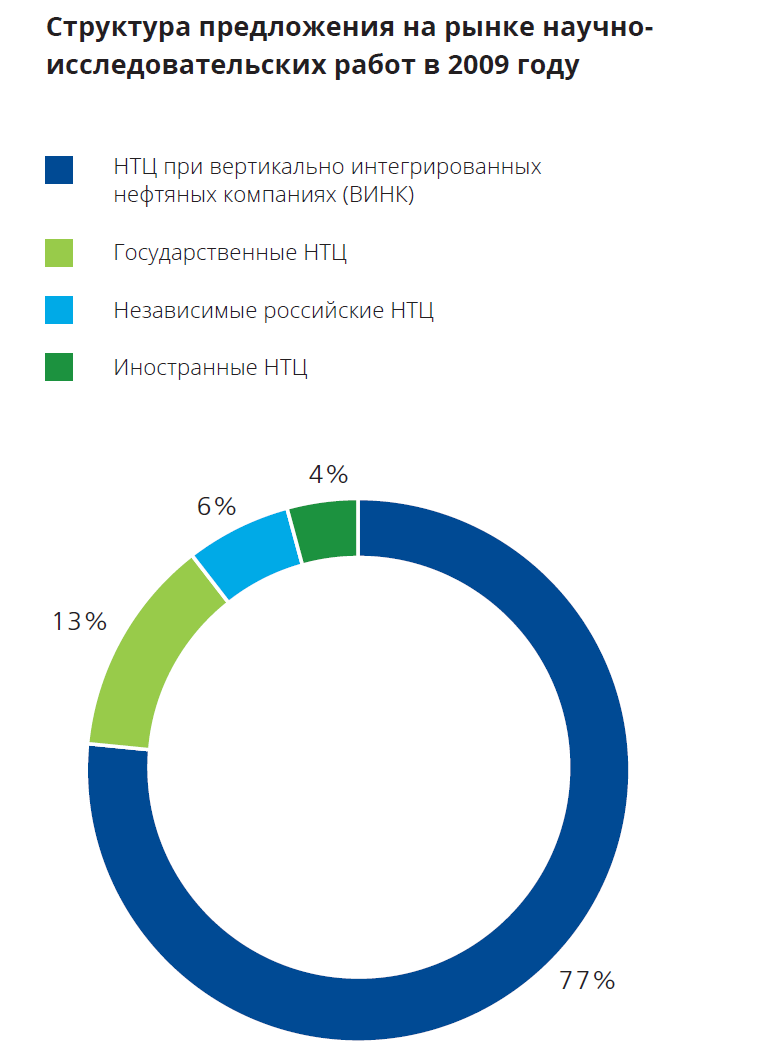
\includegraphics[width=0.8\textwidth]{int0}   
	\label{fig:int0} 
\end{figure}   

Итак, мы видим, что несмотря на определенную фактическую ориентацию отрасли на импортные технологии, доля НТЦ зарубежных нефтесервисных компаний невысока, в то время как как доля НТЦ при крупных российских вертикально интегрированных нефтегазовых компаниях превышают суммарную долю для НТЦ всех остальных типов.
Это не означает, что отрасль использует отечественные технологии, а означает лишь, что крупные игроки отрасли предпочитают осваивать и адаптировать импортные технологии своими собственными силами.
Учитывая текущую структуру рынка разработки технологий в нефтегазовой сфере России, пристальное внимание следует как раз таки уделить деятельности независимых НТЦ, причем с учетом времени их функционирования на рынке.
Так можно выявить скрытые технологические тренды и актуальные производственно-технологические запросы в нефтедобывающей отрасли России.
Разумеется, если НТЦ достаточно молод, например, функционирует на рынке не более 5 лет, то это вовсе не означает, что такая компания не может демонстрировать высокую эффективность, но при этом все же очевидно, что деятельность достаточно молодых компаний на рынке требует дополнительного анализа с точки зрения оценки эффективности и выявления перспективных трендов.

 \begin{figure}[H]
 	\caption{Операционные затраты НТЦ на одного технического специалиста, в млн рублей, 2009}
	\centering     
	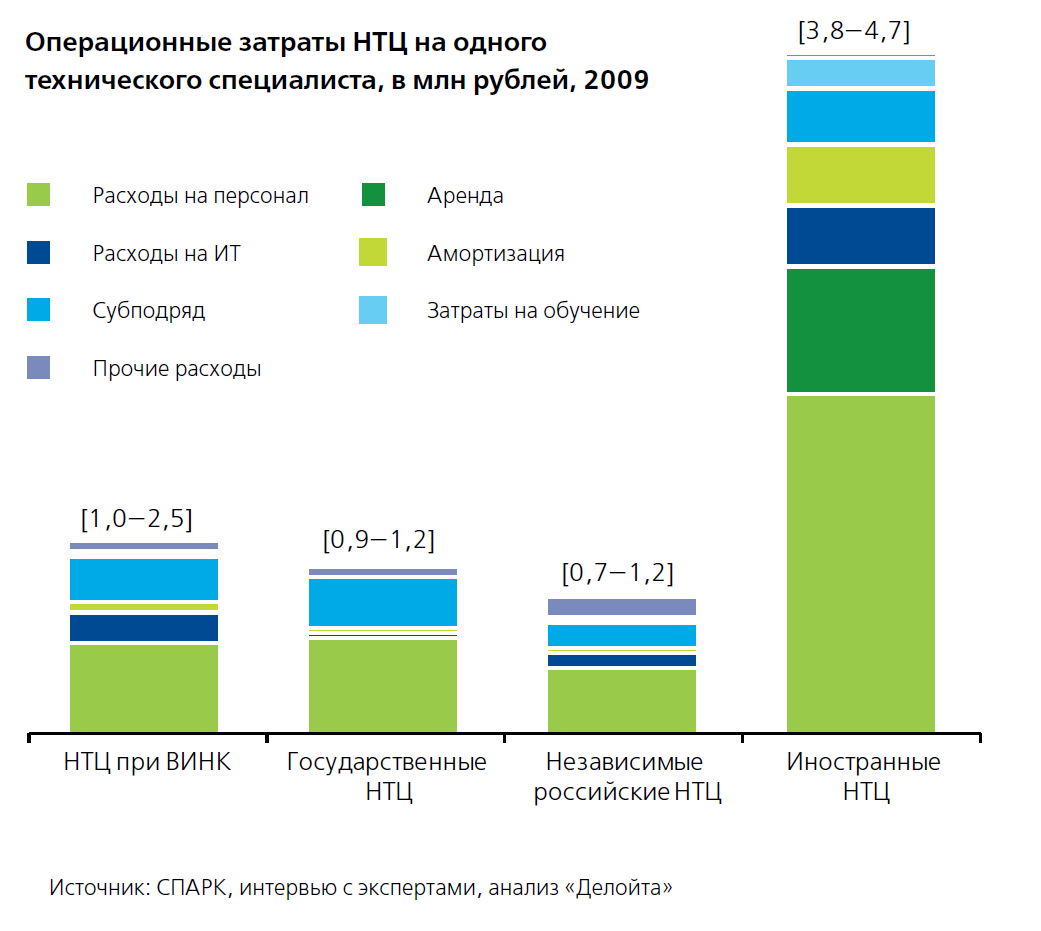
\includegraphics[width=0.8\textwidth]{int2}   
	\label{fig:int2} 
\end{figure}   

Перейдем к описанию критериев эффективности деятельности НТЦ в долгосрочном плане, связанных с собственно производимой НТЦ продукцией в виде новых технологий.
Для этого рассмотрим подход, основанный на анализе цифровых артефактов деятельности НТЦ, в первую очередь различного рода документов в электронном формате, отражающих результаты деятельности НТЦ и доступных для анализа из открытых источников.
К такого рода цифровым артефактам могут быть отнесены:  

\begin{itemize} 
	\tightlist 
	\item документы отраслевых электронных библиотек; 
	\item патенты; 
	\item статьи в отраслевых научных изданиях; 
	\item другие материалы и документы, относящиеся к деятельности нефтегазовой отрасли, имеющиеся в открытом доступе, в первую очередь в сети интернет 
\end{itemize}  

Все указанные документы могут быть подвергнуты компьютерному анализу, в первую очередь высоко-перспективным методом тематического моделирования, суть которого состоит в использовании би-кластеризации, то есть одновременной кластеризации слов и документов по их семантической близости.
При этом как правило используется скрытое размещение Дирихле, которое хотя и удобно для алгоритмических компьютерных вычислений при проведении тематического моделирования, но не вполне обосновано с лингвистической точки зрения.

Результаты тематического моделирования, проведенного автором настоящей работы, для статей во всех выпусках журнала ``Нефтегазовое хозяйство'' за период с 2008 по 2016 годы (что упоминалось уже в настоящей главе ранее) показали, что вопреки изначальному предположению о плавной эволюции выявляемых в рамках тематического моделирования тематик от номера к номеру, в различных номерах журнала были зафиксированы принципиально различные тематики.
Означает ли это, что указанный журнал в каждом новом выпуске концентрируется на новейших технологических достижениях и не производит отсылку к устаревшим и не использующимся технологическим подходам? И да, и нет.
Конъюктурная составляющая при отборе редакцией журнала публикаций с целью повышения привлекательности издания в широких кругах деятелей нефтегазовой и смежных областей очевидна.
В этом в значительной степени и состоит суть любой, в том числе и узкопрофильной, специализированной журналистики.
В то же время о судьбе упомянутых однократно технологий судить по таким однократным публикациям нельзя.
Были ли они отвергнуты в практическом применении или были опробованы и показали свою несостоятельность? 
Или, быть может, прочно вошли за анализируемый период времени длительностью в 8 лет в инструментарий нефтедобывающей отрасли? 
Такие выводы на основе проанализированной информации сделаны быть не могут.
В чем же состоит выход? 
Он состоит в анализе более широкого круга документов, от патентов до тезисов докладов на отраслевых конференциях.
Указанные документы могут быть подвергнуты кластерному анализу с применением различных алгоритмов.
При этом если речь идет об использовании классификации с обучающим шаблоном (``с учителем''), то в качестве обучающего шаблона могут быть выбраны экспертные описания основных современных технологических трендов и инновационных тематик в нефтегазовой отрасли.
Те же совокупности анализируемых документов, которые не войдут в определенные таким образом классы (кластеры), не должны рассматриваться априори как ``шум'', а должны быть подвергнуты дополнительному анализу на предмет того, что они на самом деле представляют собой свидетельства (цифровые артефакты) латентных инновационно-технологических трендов.

На базе такой выполненной кластеризации (классификации) документов (цифровых артефактов инновационно-технологического развития нефтегазовой отрасли) могут быть определены многокритериальные интегральные числовые показатели эффективности деятельности конкретных НТЦ, вычисляемые на основе долей распределения цифровых артефактов, произведенных сотрудниками данного НТЦ, по кластерам (классам).
Изменение таких распределений во времени могут служить основой для апостериорного прогнозного моделирования эффективности деятельности конкретных НТЦ в будущие периоды времени.

Отдельной темой, хотя и относящейся к технической стороне настоящего исследования, является обеспечение информационного обмена, доступа к документам (цифровым артефактам) и их предобработка, включая приведение в единообразные электронные форматы и стемминг.

Все эти вопросы и будут рассмотрены в последующих главах настоящей работы.

\section{Обзор научной литературы}
\label{cha:review}
\section{Организационная эффективность}
Гуру научного менеджмента Майкл Портер в своей книге "Международная конкуренция: конкурентные преимущества стран" \cite{porter1993m} выделяет эффективность научно-исследовательской работы как один из способов конкуренции стран. 

Существует множество подходов к трактовке понятия эффективности вообще и в научно-исследовательской работе, в частности. Но важно понимать, эффективность - это не коэффициент \cite{tikin2009e}. 

В работе \cite{kle2014o} отмечается, что научно-исследовательская работа не может быть однозначно описана и оценена с использованием унифицированных и объективных показателей продуктивности, что свидетельствует о необходимости использования сразу ряда показателей. 

В статье Левина \cite{levin2016v}, автор выступает против исключительно количественной оценки исследователей. Но несмотря ни на что, тенденция формальной оценки научных исследований продолжает распространяться в связи с отсутствием альтернативы отношению к научным текстам, как к основному продукту, производимому исследователями. При этом сам процесс производства научного текста не рассматривается в деталях в виду его творческой природы и остается ``черным ящиком''. Автор данного исследования видит в этом иррациональность и считают своей обязанностью исследовать сам процесс производства научных текстов как основу для дальнейшей оценки продуктивности научной работы и выявления возможностей для повышения продуктивности исследователей.

К основным компонентам процесса научного исследования относят формирования коллаборации исследователей, процесс создания научной статьи и ее публикации. Опубликованная научная статья является одним из воплощений результатов научного исследования. Существует множество методик ведения исследовательской деятельности. Большинство из них использует структурирование научно-исследовательской деятельности на этапы для упрощения ее понимания. Например, в книге \cite{lipch2013met} выделены следующие семь этапов:
\begin{enumerate}
\tightlist
\item Выбор темы научного исследования.
\item Изучение мирового опыта по выбранной теме посредством научных источников.
\item Составление плана научно-исследовательской работы.
\item Накопление материала для проверки обоснованности выдвинутой гипотезы.
\item Обработка данных, построение моделей.
\item Анализ результатов исследования и выводы.
\item Документальное оформление научно-исследовательской работы.
\end{enumerate}

Таким образом, создание научной статьи, как результат научного исследования, может быть представлено в виде формализованного процесса, реализуемого участниками научно-исследовательской группой. Этот процесс принадлежит к категории коллективного социального взаимодействия. И его изучение является нашей задачей в данном исследовании. Поэтому автор поставил задачу рассмотрения именно процесса совместного проведения научно-исследовательской деятельности и написания научной статьи с последующей публикацией. Кроме этого автор данного исследования постарался учесть процессы коллективного мышления и коммуникаций, отмеченные в работе \cite{mkrt1995f}.

В научной практике исследователи должны делиться результатами своих исследований с коллегами. Публикация статьи в научном журнале является одной из форм коммуникации исследователя с научным сообществом \cite{danil2016o}. Помимо публикации статьи, коммуникация может быть осуществлена в виде публикации монографии, тезисов конференций или патентов, а также личных выступлений на конференциях и семинарах. Поэтому научное исследование не может рассматриваться по мнению автора в отрыве от процесса публикации. Таким образом, в коллаборацию коллектива исследователей необходимо включить редакцию научных журналов и комитеты научных конференций.

В самом упрощенном виде редакции и комитеты конференций группируются не по формальным рубрикаторам, типа ГРНТИ, а по определенным ментальным кодам \cite{gary2016unpacking}, скрытым за описаниями формата и редакционными политиками. Примером такого кода может быть: ``Мы принимаем статьи только от членов SPE (Society of Petroleum Engineers)'' или ``Авторы должны иметь научную степень''. Понятие ментального кода широко применяется при анализе объединения в группы \cite{sidor2006g,gentner2014mental}. 
Ментальный код может состоять из отдельных фрагментов, как молекула ДНК. Важно понимать, что именно на основании совпадения ментального кода производится принятие нового участника в сообщество. Что, в нашем случае, означает принятие редакцией или комитетом конференции научной работы к публикации. Иногда часть ментального кода может быть продекларирована, но это не означает, что существенная его часть, на основании которой и будет приниматься решение не остается внутренним достоянием редакции или программного комитета. В таком случае автор будет испытывать недоумение от того, что ему ``немотивированно'' отказали, так как существенная часть ментального кода редакции или программного комитета конференции ему не доступна.

Процесс публикации научной статьи так же имеет формальные этапы, в которых, однако, не отражен сетевой процесс работы над результатом:
\begin{enumerate}
\tightlist
\item Объявление о дате и теме проводимой конференции;
\item Запрос аннотаций статей (call for papers);
\item Экспертная оценка (peer review);
\item Подготовка текста на двух языках;
\item Создание доклада;
\item Выступление с докладом;
\item Подготовка текста в формате для публикации;
\end{enumerate}

Таким образом, можно говорить о фундаментальном процессе, содержащем логику расширения группы, на основании которого работают как малые группы – соавторы, так и большие группы, включающие в общем случае представителей редакций, организационных комитетов конференций, ``гостевых авторов'', переводчиков, экспертов, осуществляющих оценку и т.п. Рассмотрение таких коллабораций необходимо для понимания процесса публикации научной статьи и последующей оценки вклада отдельных участников.

Разделение труда характеризует зрелость производственных процессов. Для рассматриваемого нами процесса написания научных статей это может означать, что создаются специализированные пулы ресурсов для поддержания определенных этапов без персонификации. Например, из прошлого нам известно жаргонное выражение ``кооператив по вписыванию формул'' применительно к кандидатским диссертациям. Несмотря на маргинальность этого явления, которое публично осуждалось и процветало за счет востребованности в узкой специализации, автор видит в нем ранние предпосылки для разделения труда в процессе производства научного исследования и публикации на его основе. В настоящее время в связи с ускорением производства научных исследований появились новые формы разделения труда (и новые требования к результативности научно-исследовательских кадров), которые нуждаются в изучении.

Вопрос коллективного создания знаний и написания научных исследований в частности имеет много аспектов, связанных с этикой исследователя. Должен ли автор, полностью выполнять все этапы работы над исследованием? Если в работе два соавтора, то какое разделение труда не нарушает этических норм исследователя? Какие роли среди соавторов этичны? В общеизвестном ``Курсе теоретической физики'' Ландау и Лифшица какую роль выполнял Л. Д. Ландау, а какую Е. М. Лифшиц?

После объединения на основе ментального кода происходит развитие отношений в рамках коллабораций в широком (с внешними участниками) и узком (в рамках исследовательской группы) смыслах. Укрепление соавторских отношений в результате написания нескольких работ создает более устойчивые рабочие группы. Существуют примеры продолжающихся на протяжении десятилетий соавторств. С другой стороны, есть примеры, когда, написав одну исследовательскую работу, авторы больше не сотрудничают. В чем причины устойчивых объединений в соавторские коллективы?

Автор считает, что во многих научно-методических источниках основное внимание уделено технологиям написания научной статьи и ее оформлению, но не изучению процесса создания научных статей, поэтому считают данную работу практически полезной для администрирования и планирования НИР в понятиях научного менеджмента по системе Тейлора \cite{taylor2004scientific} .

Проблема объективной оценки эффективности НИР находится в центре внимания исследователей уже давно, и это, в первую очередь, связано с вопросами финансирования как бюджетного, так и в рамках грантов. В рамках традиционного подхода выделяются следующие индикаторы оценки эффективности \cite{korol2014krit}:

\begin{itemize}
\tightlist
\item Финансовые
\item Кадровые
\item Инновационные
\item Библиометрические
\end{itemize}

Собственно в рамках библиометрии учитываются следующие параметры:

\begin{itemize}
\tightlist
\item число публикаций в международных журналах характеризует качество статей; 
\item индикатор цитирования и индекс Хирша показывают степень значимости проводимых исследований и признание научных школ мировым сообществом;
\item ``публикационная нагрузка'' ученых – продуктивность ученых; 
\item наличие патентов; 
\item соавторство с зарубежными учеными – показатель международной кооперации''.
\end{itemize}

Как отмечают многие исследователи \cite{vonortas1995new, veugelers1998collaboration, faems2005interorganizational }, этот набор параметров далек от совершенства, поскольку не даёт полностью объективную картину НИР выбранного учёного или коллектива. Например, индекс Хирша зависит от дисциплины, а также он не спадает, если человек не публиковал новых работ в течение 10 и более лет. Цитатные базы WoS и Scopus, во-первых, неполноценно отражают исследования на русском языке, а во-вторых, разным дисциплинам отводятся в них неравные доли. 
В данном исследовании проверяется гипотеза, что повышение качества оценки эффективности НИР возможно через учёт дополнительных факторов, о которых будет сказано далее.

Эффективность организации – очень сложный и многогранный концепт. 
На него оказывают влияние различные факторы. 
Одним из важных предвестников рыночного успеха научно-исследовательской компании является хорошо развитая коммуникация и кооперация между сотрудниками. 
Многие теоретические и практические исследования демонстрируют связь между продуктивностью организации и структурой коммуникации её сотрудников, например,  в работах  \cite{allen1984managing,noe2006human}.
Исследование социальной структуры организаций и профессиональных сообществ становится одним из главных направлений прикладного анализа социальных сетей. 
В сфере общественных связей и управления глубоко изучаются модели коммуникаций внутри организаций. 
Начало этим исследованием положено в 1956 году работе C.H.Cooley ``Социальная организация'' \cite{cooley1956social}.

Информация о взаимодействиях сотрудников может быть получена различными способами, например, с помощью корпоративных баз данных, общественных опросов и личных отчётов. 
Однако, данные, полученные такими путями, нужно интерпретировать с некоторыми оговорками, поскольку они не отражают всего механизма профессионального взаимодействия в целостности. 
Как утверждают Вассерман и Фауст \cite{wasserman1994social}, около половины того, что люди сообщают о своих взаимодействиях, по той или иной причине неправильно. 
Таким образом, людям не очень хорошо удаётся качественно информировать о своих взаимоотношениях, поэтому пути сбора данных должны избегать такой субъективности.

Источником такой информации может быть Google Scholar, arXiv и другие онлайн библиотеки. 
Рассмотрение открытых научных сообществ так же интересно, как и сужение выборки до одной страны, отрасли и организации. 

Одним из более объективных способов анализа человеческих взаимодействий является формальный концептуальный анализ (англ. formal concept analysis, FCA). 
FCA представляет собой определенный способ анализа коллекции объектов и их свойств. 
Идея применить FCA в области анализа социальных сетей уже не нова. 
В работе \cite{kurtz2009c} он был использован для массового анализа сети. 
В \cite{snasel2009analyzing} комбинация формального концептуального анализа и известных методов факторизации была направлена против вычислительной  сложности анализа социальных сетей, а также на облегчение визуализации этого анализа. 
Би-кластеризация и три-кластеризация были применены в \cite{gnatyshak2012gaining} для анализа данных, собранных в русской социальной интернет-сети Вконтакте для выделения групп пользователей со схожими интересами, для поиска сообществ пользователей, входящих в состав схожих групп и для выявления интересов пользователей. 
Формальный концептуальный анализ многократно использовался для анализа социальных сетей, основанного на ссылках \cite{kuznetsov2007reducing}, 
для обнаружения криминальных сетей \cite{poelmans2012semi}. 
Другие способы применения FCA можно почерпнуть в работе \cite{poelmans2013formal}. 
Весьма подробный анализ приложений на основе FCA для анализа социальных сетей можно найти в \cite{aufaure2013advances, obiedkov2007social, pensa2005towards}.

Одним из частных случаев коммуникации является кооперация, которая может в случае научно-исследовательской работы переходить 
в соавторство при создании научных публикаций. 

Публикация научных исследований – главный объект, по которому оценивается эффективность научно-исследовательской работы. 
Поэтому важно проследить, как проходит этот процесс, начиная с зарождения исследовательской идеи, проведения эксперимента и заканчивая публикацией работы. 
Необходимо провести анализ, какие условия способствуют успешной публикации статьи. 
В рамках данного исследования было изучено соотношение публикаций отдельных учёных и научных коллективов. Было показано, что за последнее десятилетие есть чётко выраженная тенденция ученых объединяться в группы соавторов для публикации статей. 
Отсюда можно сделать вывод, что одним из факторов, положительно влияющих на опубликование работ, является объединение людей в команды.

В свою очередь, командообразование тоже бывает успешным и неуспешным, оно также поддаётся изучению, в результате которого можно выделить условия успешного командообразования. 
Задача поиска оптимальных параметров команды соавторов для наиболее продуктивного написания научных статей относится к классу задач оптимизации. 
Традиционно исследователи обращают внимание на следующие параметры, имеющие значение для продуктивного научного творчества:
\begin{itemize}
\tightlist
\item Размер команды         
\item Ментальные модели сообщества
\item Компетенции сотрудников (дополняющие и гомофильные)
\item Слабые связи между учёными
\end{itemize}

В отличие от размера команды, который является явным, а не скрытым признаком, а также легко формализуемым, 
признак ментальных моделей (англ. mental model) сообщества гораздо труднее поддаётся выявлению и фиксации. 
Многие исследователи отмечают важность изменения во времени ментальных моделей помимо структуры команды \cite{klimoski1994team, morgeson1999structure}. 
Понятие ментальной модели является развитием понятий структуры знания \cite{walsh1995managerial}, схемы знаний \cite{fiske2013social, sims1986thinking}, и неявной теории \cite{brief1983cognitive}. 
Автор данного исследования трактует понятие ментальной модели как стратегическую согласованность командных компетенций. 
Например, ментальная модель ``Agile geoscience'' \cite{hall2011shale} крупнейшего сообщества ученых-геофизиков основывается на компетенциях ``гибкие методики'' и ``геология''.

Исследователи сходятся в том, что совпадение ментальных моделей участников команды положительно влияет на производительность \cite{lim2006team, mathieu2000influence}. 
Этот факт говорит о связи ментальной модели команды и полного командного кода, которое более подробно раскрыто далее. 

Формирование основной системы внутреннего взаимодействия внутри команды согласно исследованию \cite{harper1985power} происходит при знакомстве участников по принципу дополняемости.
Тем не менее, нельзя полностью отрицать значение гомофильных (совпадающих) компетенций. 
Во многих работах отмечается динамическая структура гомофилии \cite{mcpherson2001birds, snijders2010introduction, steglich20108}, в ходе которой параллельно происходят два процесса. 
С одной стороны – схожие между собой индивиды формируют социальные связи (социальная селекция). 
С другой – уже связанные друг с другом люди перенимают поведение друг друга (социальное влияние). 
Совокупность этих факторов результирует в гомогенную социальную систему, 
в которой между индивидами со схожим поведением и характеристиками есть связь, при этом характер связи может быть, как формальным, так и неформальным.                     

Несмотря на то, что связи между индивидами со схожими характеристиками более вероятны, чем связи между непохожими, уровень схожести также важен. 
В работе \cite{block2014multidimensional} было показано, что социальная схожесть более, чем по одному показателю, 
приводит к тому, что люди с меньшей вероятностью будут формировать между собой взаимоотношения. 
Автор объясняет данный эффект тем, что слишком схожие по многим характеристикам люди, как правило, 
не могут привести что-то новое и конструктивное во взаимные отношения или же в команду. 

Для продуктивного сотрудничества необходима не только схожесть интересов, 
но также и различный профессиональный и жизненный опыт, позволяющий предложить многомерные подходы к ее решению.

\section{Место текста в научной деятельности}
Анализ текста иногда называют \textit{Text Mining}. Суть этого процесса в превращении данных (текста) в высоко-качественную информацию способную приносить знания. Важным моментом является то, что при получении знаний человеческие затраты должны быть минимальны. 

Полученные из текста знания становятся основой для принятия управленческих решений в организационной среде. 
Отдельным процессом рассматривается получение текста, иногда называемое созданием корпуса текстов. 

Реальный мир находит свое отражение в текстах при помощи авторов, а процесс анализа текста делает обратное: на основе текстов составляет информацию о реальной природе вещей. 

Многомодовым подходом к анализу текстов называют процесс учитывания сопутствующей основному тексту информации. Например адрес письма, номер выпуска газеты с новостями или фамилии соавторов научной статьи. 

Формально анализ текста производится в следующей последовательности: 
\begin{enumerate}
\tightlist
\item анализ языка текста
\item анализ содержания текста
\item получение информации об авторе текста
\item вывод определенных переменных, характеризующих природу вещей в тексте
\end{enumerate}

Рассмотрим более подробно методы работы с текстами научных статей.

\subsection{Обработка текста}
Задачи по обработке текста были поставлены в 60-70 годах 20-ого века при обработке натурального языка \cite{weizenbaum1966eliza, kuvcera1967computational}.
Нужно было приводить текст к более удобной для последующего анализа форме. Эту процедуру общепринято называть \textit{нормализацией текста}. Для нормализации текста  использовались регулярные выражения (regular expressions), концепцию которых разработал С.К.Клини \cite{kleene1951representation}. Одним из первых, кто использовал регулярные выражения в работе с тестом был К.Томсон \cite{thompson1968programming}.

В настоящее время задачи нормализации текста существенно расширились. Нужно не только выделять слова, но и учитывать специальные символы, обозначающие эмоции (Emoji), такие как 8-) \cite{eisner2016emoji2vec}, выделять хештеги \cite{o2010tweets},  выделять гиперссылки \cite{bingel2017identifying} и обрабатывать цитирования \cite{jha2017nlp}.
	
Задача лексического анализа состоит в разделение текста на части - предложения, слова, буквы.  Иногда лексический анализ называют токенизацией от английского слова \textit{tokenizing} \cite{lovins1968development}.

Другая задача нормализации текста состоит в определении слов с единой основой и называется лемматизацией. Основа слова не обязательно совпадает с морфологическим корнем слова. 
Лемматизация для русского языка отличается от лемматизации для английского \cite{segalovich2003fast, sharoff2011proper, korobov2015morphological}. Поэтому для английского языка используют процедуру лемматизации на основе частотных алгоритмов \cite{willett2006porter, porter2001snowball}, так же называемую стемминг от английского слова \textit{stemming}. Но для других языков лемматизация использует еще более сложные алгоритмы. Например, есть стемминг для Древнегреческого языка \cite{packard1973computer}.

Таким образом нормализация текста состоит из трех этапов: 
\begin{enumerate}
\tightlist
\item Выделения слов из текста
\item Приведения слов к более общим формам 
\item Выделении предложений 
\end{enumerate}

Для автоматизации задач нормализации текста используют библиотеки на языке программирования Python. Например, библиотеку NLTK \cite{bird2009natural}, содержащую огромное количество различных алгоритмов обработки текста.

\subsection{Модели текста}
\label{sec:textmodel}
Модели, которые присваивают вероятности словам в последовательностях слов называются вероятностными моделями текста. Математически это определение можно записать в виде уравнения. 
Допустим у нас есть вероятность последовательности из $n$ слов $ P(w_1, \dots, w_n)$, такая, что вероятность третьего слова $P(w_3) $ равна $P(w_3|w_1,w_2)$. 
Тогда следующее выражение определяет вероятностную модель текста. 

\begin{defi}[О\ref{defi:rev1}] 
\label{defi:rev1}
$$P( w ) = P( w_1, w_2, \dots , w_n ) =  \prod_i^n P( w_i | w_1, w_2, \dots , w_{i-1} )$$
\end{defi}

Так как вычисление $P (w) $ представляет сложность $O^n$, то современные исследования текста используют представление $P ( w )$, как однородной Цепи Маркова и строят приближенные модели \cite{schwenk2002connectionist}: 

\begin{enumerate}
\tightlist
\item Униграмная модель $ P(w_1, w_2, \dots , w_n )  \approx \prod_i P(w_i)$
\item Биграмная модель $ P(w_i \vert w_1, w_2, \dots , w_{i-1} )  \approx  \prod_i P(w_i \vert w_{i-1} )$
\end{enumerate}

Можно так же рассматривать n-грамные модели для большего охвата контекста, как в работах \cite{teahan1996entropy, teahan1997models}. Применительно к задачам распознавания речи это сделано в работах исследователей из ИБМ \cite{bahl1983maximum, bahl1986maximum, averbuch1987experiments}.

Tomas Mikolov в работах \cite{mikolov2013efficient,mikolov2013distributed} показывает, что и эти упрощенные модели обладают слишком большой вычислительной сложностью, поэтому его лаборатория разработала векторное представление слов не с помощью априорных распределений как в исследовании \cite{blei2006dynamic}, а на основе встраиваемых (embedded) векторов. 

Из определения (О\ref{defi:rev1}) следует и способ для проверки качества вероятностной модели текста. Для этого пользуются метрикой \textit{Perplexity}: 

\[ 
\mathcal{P}  = \sqrt[n]{\frac{1}{P(w)}}
\]

В работах \cite{cover1991entropy, algoet1988asymptotic} показано, что между метрикой \textit{Perplexity} и относительной энтропией на одно слово $  H(W)$ существует следующая зависимость: 

\[
 H(W) = \log_2 Perplexity(W) 
\]

Клод Шеннон \cite{shannon1951prediction} оценил энтропию  английского языка как 0.6 - 1.3 бита на букву, прося людей предсказать следующую букву слова. 
В работе \cite{cover1978convergent} дана оценка нижней границы энтропии английского текста как 1.25, а в работе \cite{brown1992estimate} с использованием триграм модели слов приведена оценка 1.75 бит на слово.  

Но есть и другие подходы к оценке качества моделей текста. Например в работах \cite{cohen1998learning, collobert2011natural} использует метрику основанную не на энтропии, а на попарном сравнении (pairwise ranking approach).

Помимо подхода, развиваемого T.Mikolov, существуют и другие способы векторного представления слов. Следует отметить работу исследователей и Университета Стандфорд, названную GloVe \cite{pennington2014glove}. Векторное представление слов Glove требует существенно меньше вичислений, так как использует только частоты употребления слов, а не вероятности.  

\subsection{Классификация текста}
\label{sec:textclassification}
Самым распространенным примером потребности в классификации текстов, наверное, является задача отнесения писем к категории нежелательных почтовых рассылок, называемых спамом. И базовой линией для этой задачи является классификатор на основе алгоритма Наивный Байес (НБ).

Наивная Байесовская текстовая классификация была предложена М.Мароном в работе \cite{maron1961automatic} для присвоения категории принадлежности текста доклада определенному журналу. 
Его модель представила большинство особенностей, используемых и в настоящее время для задач классификации текстов. 

Байесовские методы \cite{bayes1763essay} были также применены к задачам классификации текстов по авторству в пионерской работе Ф.Мостеллера и Д.Уоллеса \cite{mosteller1963inference}. 
Наивный Байес был впервые применен для обнаружения спама в работе \cite{sahami1998bayesian}.

В работах \cite{metsis2006spam, wang2012baselines, pang2002thumbs} было показано что, использование бинарных признаков с мультиномиальным распределением дает лучшие результаты, чем счетчики слов. 

Бинарный Байес с Мультиномиальным распределением часто путают с другим вариантом наивных Байесовских алгоритмов, которые также используют двоичное представление того, встречается ли слово в документе: Многовариантный Наивный Байес (МНБ) с использованием распределения Бернулли. 
Вариант НБ с рапределением Бернулли оценивает вероятность того, что слово не входит в документ. 

В исследовании \cite{mccallum1998comparison} показано, что МНБ не всегда хорошо обобщается на новые тексты.

Задача определения эмоциональности текста относится к задачам классификации и успешно решается с помощью алгоритмов НБ.  
Существует ряд хороших обзоров применения анализа эмоциональности текстов среди которых работы \cite{pang2008opinion, liu2012survey, stamatatos2009survey}.

Стоит также отметить хороший обзор различных текстовых классификаторов, сделанный К.Маннингом с соавторами \cite{schutze2008introduction}.

В настоящее время векторное представление частей текста (embedding)
приобрело большую популярность. Широко используются методы Word2Vec
\cite{mikolov2013efficient}, GloVe \cite{pennington2014glove},
StarSparse \cite{wu2017starspace}, Fasttext \cite{bojanowski2016enriching}, Sent2vec
\cite{pagliardini2017unsupervised}. 
Поэтому стоить упомянуть и рациональный взгляд на преимущества
от использования векторного представления  

Основной демонстрацией преимущества от использования векторного
представления слов стала формула: king - men = queen.
Смысл этой формулы в том, что векторные представления слов (king, men, queen) можно подвергать арифметическим операциям. 

Но отнюдь не все слова так складываются. Некоторые очевидные для человека аналогии в векторном представлении не являются близкими векторами \cite{finley2017analogies}.
Поиск смыслов в векторных представлениях предпринят в работе \cite{pelevina2017making,panchenko2017unsupervised}.

Алгоритм AdaGram предложен в работе \cite{bartunov2016breaking} для  поиска векторных представлений для неоднозначных слов.
Исследование уточнения пониманий векторных представлений в зависимости от контекста предпринято в работах \cite{huang2012improving,gladkova2016intrinsic}. 
 
Существенные преимущества в классификации текстов были получены от применения рекуррентных нейронных сетей. 
Из всей массы работ в этом направлении необходимо отметить многочисленные исследования текстовых моделей на основе нейронных сетей
выполненные сотрудниками лаборатории естественного языка при Стенфордском университете \cite{schuster2018gapping,eric2017copy,wang2017naturalizing,li2017adversarial,xie2017data}.

\section{Анализ социальных сетей}

В книге \cite{de2018exploratory} отмечается, что базисом для анализа социальных сетей является теория социометрии, основанная J.L.Moreno \cite{moreno1953shall}. 
Социометрия изучает взаимоположения социальных атомов в группах. 
Социограммой по Морено является графическое отображение социального выбора членов социальной группы.
Социальным выбором может быть выбор лидера, дружба, выполнение совместных задач, и др. 
Социограма представляет граф, состоящий из вершин и ребер. 

В книге \cite{tsvetovat2011social} M.Tsvetovat  с соавторами ставит вопрос:
Кто из участников организации, представленной в виде графа, важнее? 
Таким образом проводя логическую связь между графами и организационной теорией, что отмечено в работе \cite{atherley2015model}.

Хорошим примером измерения инновационности организации с помощью анализа социальных связей служат исследования \cite{porter2018mapping} .

Направление углубленного изучения графов (Social media mining) деятельных сообществ развито в работах \cite{kurmukov2016classification,zafarani2014social}. Таким образом, переводя различные метрики графов в свойства для задач классификации составляющих графы вершин и ребер. 

Например, в работе \cite{makarov2016co}  метрики графа соавторства использованы для предсказания новых соавторств.
А в работе \cite{makarov2018recommending} предсказание соавторств использовано для повышения эффективности научной организации.

Для решения задач предсказания вершин и ребер графов необходимо рассмотреть, как создаются графы.
Известны модели Small World \cite{watts1998collective}, Preferential Attachment Model \cite{barabasi1999emergence}, и другие модели случайных графов, состоящих из подграфов.

В работе \cite{fortunato2010community} показано, что выделение подграфов дает возможность выявления социальных подгрупп, объединенных общей темой. 
Определение таких сообществ не представляется возможным без использования матетамического аппарата теории графов \cite{lancichinetti2009community}. 

Одной из методик для выявлении сообществ является построения векторного пространства узлов (node embedding) \cite{zheng2016node}. Так же как и с векторным пространством частей текста, описанным в разделе \ref{sec:textclassification}, построение векторного пространства узлов позволяет вводить авторам исследования \cite{liu2017semantic} новые свойства графов на основе близости узлов в векторном пространстве.

Граф соавторства является частным случаем социальной сети. 
Одним из первых исследований графа соавторства является работа \cite{mullins1973development}, сделанная в 1973 году.
С этого времени исследования научной деятельности при помощи графов соавторства не прекращались и обрели статус проверенного инструмента анализа. 
Например, в недавнем исследовании \cite{chuan2018link} предпринята попытка предсказания будущих научных исследований на основе графа соавторства, а в работе \cite{chen2017building} построен глобальный граф соавторства на основе Google Scholar, который содержит более 400 тысяч вершин. Оба исследования проведены в 2017 году.

Построение графа соавторства выполняется таким образом, что если два автора сделали совместную научно-исследовательскую работу, то каждый из авторов считается вершиной графа, а факт соавторства ребром графа. 
Будем называть такой способ создания графа соавторств традиционным. 
В результате такого, традиционного подхода получают граф, изображенный на рисунке (Рис. \ref{fig:rev1}).

\begin{figure}[H]
  \centering
  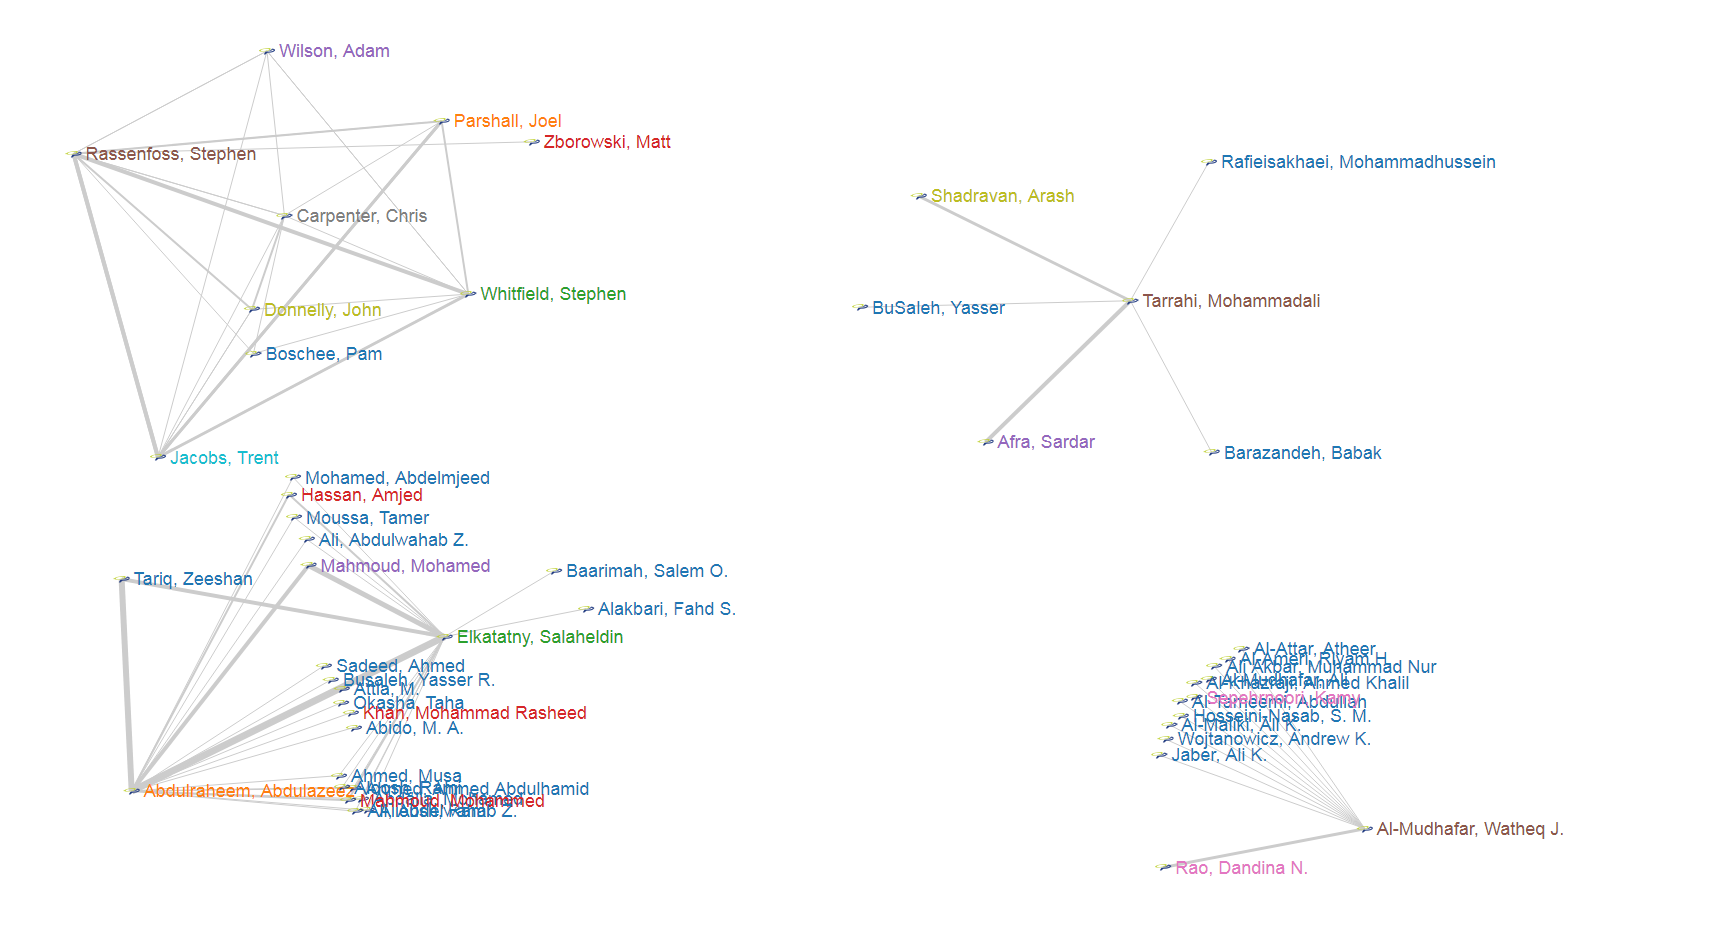
\includegraphics[width=0.8\textwidth]{rev1}
  \label{fig:rev1}
  \caption{Пример простого графа соавторства.}
\end{figure}

\chapter[Объект и метод]{Объект и методы исследования}
\label{cha:objectandmethod}

\section{Цифровые экосистемы}
Появление цифровых экосистем является результатом естественного развития научного сотрудничества и информационных технологий. 
Целью цифровых экосистем является повышение эффективности связей между внутренними и внешними агентами для поддержания бизнеса. 
В литературе есть два широких определения концепции цифровых экосистем. 
Первое исходит из структурной и функциональной перспективы, которая видит цифровую экосистему как открытую сетевую среду для эффективного взаимодействия. Второе, напротив, рассматривает цифровую экосистему как открытый кластер слабо связанных компонент, в котором каждый агент является проактивным для собственной выгоды (Рис. \ref{fig:om0}).

\begin{figure}[H]
  \label{fig:om0}
  \centering
  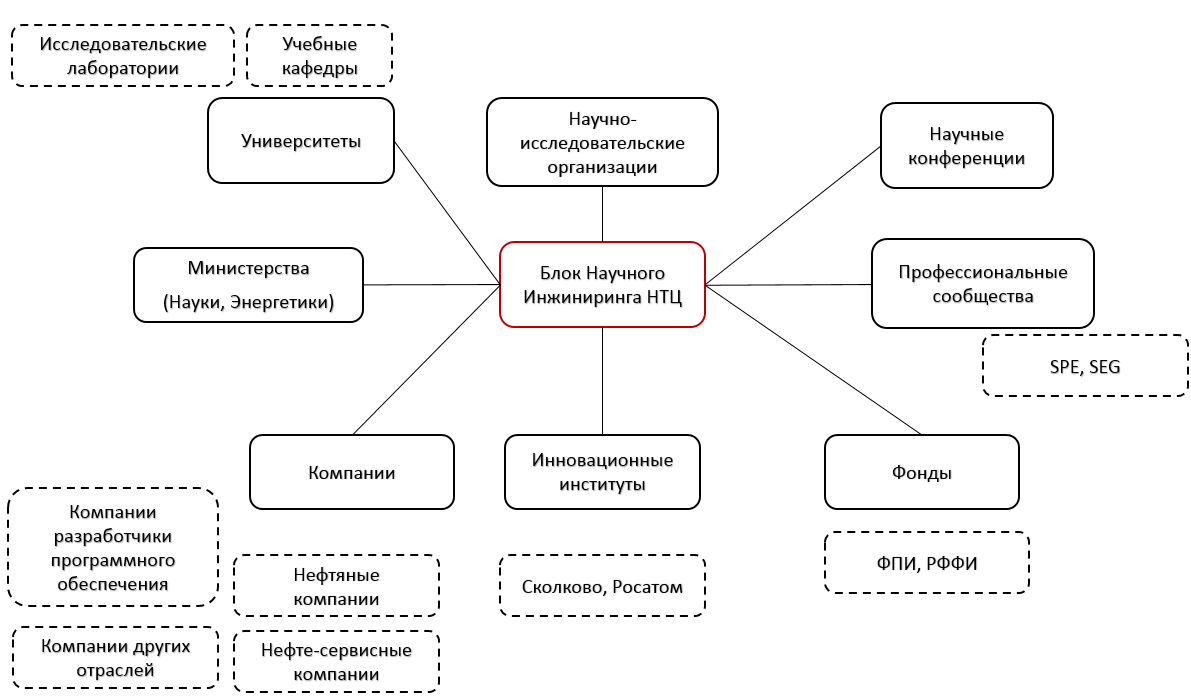
\includegraphics[width=0.8\textwidth]{se_eco}
  \caption{Экосистема научного инжиниринга}
\end{figure}

Понятие ``цифровые артефакты'' вошло в обиход вместе с понятием цифровой экосистемы. 
В широком смысле цифровые артефакты являются синонимами любых информационных результатов действий цифровой экосистемы. 
По своей информационной природе цифровые артефакты могут сохраняться или разрушаться.
Как при сохранении, так и при разрушении происходит видоизменение изначального цифрового артефакта. 
В исторической перспективе цифровые артефакты могут быть изучены, как и любые другие продукты деятельности человека.

Цифровые экосистемы можно рассматривать на макроуровне (страна, отрасль) и на микроуровне (корпорация, группа компаний, отдельное предприятие, департамент). Цифровые артефакты также могут существовать на разных уровнях. 

Одним из примеров цифровых артефактов на микроуровне являются системы распространения знаний в нефтегазовых компаниях.
Система распространения знаний (СРЗ) – это инструмент, помогающий координировать процессы управления и обмена знаниями в области разведки и добычи нефти внутри группы компаний ``Газпром нефть'' для решения технологических и производственных задач при принятии решений. 

Она предназначена для настройки процессов сбора, обработки и распространения знаний с целью извлечения максимальной выгоды от внедряемых в компании практик и технологий.
СРЗ реализована в виде информационной системы с несколькими модулями, помогающими получить необходимую информацию по разным аспектам работы на месторождении. 

В СРЗ систематизировано представлена информация о лучших практиках, применяемых в ``Газпром нефти'' в области разведки и добычи. Система позволяет пользователю проводить сравнительный анализ и подбор оптимальных технических решений в соответствии с необходимыми ему критериями. В ней также хранятся данные обо всех проведенных внутри компании испытаниях нового оборудования, что позволяет наиболее эффективно внедрять новое оборудование и технологии на любом месторождении внутри компании. 

Наибольший вклад в развитие СРЗ вносят эксперты Научно-Технического Центра ``Газпром нефти''. Они формируют крупную структурированную базу знаний по различным областям геологии, геологоразведки и добычи, к которой имеют доступ все сотрудники ``Газпром нефти''. СРЗ – это один из инструментов создания инновационного климата внутри компании, необходимого для развития новых, более эффективных технологий разведки и добычи нефти. 

\section{Модели и моделирование социотехнических объектов}

Современная парадигма научного исследования заключается в том, что реальные объекты заменяются на их упрощённые представления, абстракции, выбираемые так, чтобы в них отражалась сущность явления, те свойства исходных объектов, которые являются существенными для решения проблемы, которая была поставлена. 
Объект, который построен вследствие упрощения, называют моделью.

Модели могут классифицироваться по разным признакам: динамические и статические, дискретные и непрерывные, стохастические и детерминированные, имитационные и аналитические. 

Статистические модели оперируют характеристиками и объектами, которые не меняются во времени. 
В динамических моделях изменение параметров модели во времени является существенным.
Статистические модели имеют дело с уравнениями балансового типа, установившимися процессами, с предельными характеристиками.
Моделирование динамических систем заключается в имитации правил перехода системы из определённого состояния в другое в течение времени.

Модели, у которых состояние изменяется непрерывно во времени, называются непрерывными. 
Модели, у которых переходы от одного состояния системы в другое происходят мгновенно, в дискретные моменты времени, называются дискретными.

Стохастические модели, в отличие от детерминированных, учитывают вероятностный характер параметров системы.

При аналитическом моделировании процессы функционирования исследуемой системы отражаются как алгебраические, интегральные, дифференциальные уравнения и логические соотношения, и в определённых случаях анализ таких соотношений может выполняться посредством аналитических преобразований.

При имитационном моделировании структура моделируемой системы -- её связи и подсистемы -- непосредственным образом представлена структурой модели, а процесс функционирования подсистем в виде уравнений и правил, которые связывают переменные, имитируются на компьютере.

Компьютерные системы предсказательного моделирования (которые также называются системами поддержки принятия инженерных решений) с компьютерными системами проектирования давно применяются в целях автоматизации трудовой деятельности инженера-проектировщика и повышения качества решений, которые принимаются. 
Но до начала XXI века в предсказательном моделировании применялись исключительно математические модели, основанные на принципах физики, описывающие физические явления и процессы, которые происходят при функционировании объекта, сложными дифференциальными уравнениями в частных производных с граничными условиями. 
В содержательных ситуациях для таких уравнений неизвестны ни теоремы о единственности и существовании решения, ни характер зависимости решения от граничных условий и параметров.
Численные методы решения этих уравнений обладают значительной вычислительной трудоёмкостью и самих расчётов, и подготовки исходных данных и расчётных сеток.
В силу этого существенно сокращаются возможности использования этих моделей в проектировании сложных объектов, в особенности на этапе концептуального или предварительного проектирования, когда рассматривается значительное число разных вариантов решений и особенно высока цена решения, которое выбрано неправильно. 
Важная часть предсказательного моделирования -- это имитационное моделирование, которое используется для исследования сложных информационно-телекоммуникационных систем.

\subsection{Апостериорный и априорный подходы к исследованию}
Рассматривая возможности апостериорного и априорного подхода к исследованию, автор склоняется к тому, чтобы отдать первенство экспериментальному изучению данного явления, а потом выяснить, какие из теорий смогут составить базу для дальнейшего углубления в изучение феномена соавторства.

Современные возможности прямого имитационного моделирования стали настолько удобны для произведения вычислительных экспериментов, что для начального подхода к изучению сложных социальных явлений достаточно быстро могут дать исследователю существенное понимание их природы. Формализм математической модели в данном случае не абстрагирует в мир греческих букв, а приближает к пониманию родовых особенностей исследуемого объекта.

Модель стремиться дать то описание системы, для которого она создается. 
Но отметим, что создание модели для полного описания социальной системы не является корректной постановкой задачи. 
Полная модель социальной системы будет настолько же сложна, насколько и сама социальная система. 
Сформулируем следующее определение модели социальной системы (О\ref{defi:so1}):

\begin{defi}[О\ref{defi:so1}] \label{defi:so1}
Модель  $\mathbb{M}_{\Omega}$ социальной системы $\Omega$ может быть использована для получения характеристик $\mathbb{RE}$ с некоторой точностью $\delta$.
\end{defi}

Таким образом, целью модели является получение ответов на некоторую совокупность вопросов. 
Эти вопросы неявно присутствуют (подразумеваются) в процессе анализа, и, следовательно, они руководят созданием модели и направляют его. 
Это означает, что сама модель должна будет дать ответы на эти вопросы с заданной степенью точности. 
Если модель отвечает не на все вопросы или ее ответы недостаточно точны, то говорят, что модель не достигла своей цели.

Агентное моделирование предполагает имитацию поведения системы путем настройки поведения отдельных агентов. 
На основании результатов поведения отдельных индивидов складывается комплексная картина взаимодействий. 
Метод агентного моделирования используется в дополнение к методу системной динамики, в рамках которой моделируется поведение всей системы в целом.

Программные алгоритмы агентного моделирования разработаны в нескольких информационных системах, в частности Anylogic и NetLogo.
Для решения практических задач эти информационные системы используется в социальных науках, в том числе в экономике и социологии. 
Важной задачей агентного моделирования является включение информации о взаимодействиях агентов между собой, так как в некоторых социальных системах именно комплексная структура взаимодействий индивидуальных агентов и приводит к более сложным макро-состояниям. 
Агентное моделирование используется для изучения динамики социальных сетей и взаимного влияния экзогенных и структурных характеристик друг на друга.

Модель для исследования взаимодействия агентов в процессе создания научных статей была реализована автором в программной среде агентного моделирования AnyLogic, базирующемся на языке Java. 
В среде AnyLogic для каждого из агентов прописываются определенные правила поведения – эвристики, индивидуальные стратегии.
После того, как для каждого из агентов прописываются все правила поведения, запускается серия симуляций.
Программные среды для агентного моделирования используются для предсказания коллективного поведения, массовых мероприятий, учебного процесса и многих других социальных процессов.

Для моделирования процессов в данном исследовании использовался метод имитационного моделирования на основе внутренних состояний и действий.
Основное преимущество данного подхода состоит в возможности проведения компьютерного эксперимента для понимания поведения системы в целом с помощью настройки графов состояний и действий децентрализованных индивидуальных агентов. 
Таким образом, в результате была получена база данных поведения агентов для исследования процессов.

В рамках изложенной выше методологии были сформулированы следующие вопросы для исследований:
\begin{enumerate}
\item В какой степени научная статья отражает проведенную НИР? Можно ли судить о качестве НИР по опубликованным научным исследованиям?
\item Каковы социальные механизмы объединения исследователей для проведения НИР? Какие виды компетенций и в какой степени влияют на такое объединение?
\item Как зависит время проведения НИР от количества участвующих исследователей? Существуют ли естественные ограничения на количество и состав исследовательских групп и на чем они основаны?
\item Каковы эвристические алгоритмы поведения исследователей по отношению к издательствам и программным комитетам конференций? Существуют ли базовые стратегии поведения? Если возможность идентификации и имитации базовых стратегий?
\item Применимы ли подходы time management (``управление временем'') к НИР? Насколько эффективно рассмотрение научно-исследовательской деятельности как проектной деятельности?
\item Какова модель зрелости научно-исследовательской организации в части проведения НИР? В какой степени возможно определение степени зрелости научно-исследовательской организации на основе анализа публикуемых ею научных статей?
\item Какова структура процессов, составляющих научно-исследовательскую деятельность? Насколько применим процессный подход к изучению научно-исследовательской деятельности? Есть показатели научно-исследовательской деятельности, отражающие характерную структуру составляющих ее процессов?
\end{enumerate}

\subsection{Теория имитационного моделирования}

Имитационное моделирование является методом исследования, при котором изучаемую систему заменяют на модель, которая с достаточной точностью описывает реальную систему, с которой проводятся эксперименты для получения информации об этой системе.

Цель имитационного моделирования заключается в получении приближенных знаний об определенном параметре объекта, без осуществления непосредственного измерения его значений. 
Такая необходимость возникает, когда измерение невозможно или оно стоит дороже, чем проведение имитации.
В то же время для изучения такого параметра есть возможность пользоваться иными известными параметрами объекта и моделью его конструкции.
Допуская, что модель конструкции довольно точно описывает объект, автор предполагает, что статистические распределения значений параметра моделирующего объекта, полученные в ходе имитации, будут в определённой степени совпадать с распределением значений параметра реального объекта.

Направления применения имитационного моделирования:

\begin{itemize}
\tightlist
\item  Агентное моделирование
\item  Системная динамика
\item  Дискретно-событийное моделирование
\item  Динамические системы
\end{itemize}
%Нужна какая-то завершающая фраза, подводящая итог этому разделу и вводящая в следующий.
Далее рассмотрим более подробно Системную динамику.

\subsection{Системная динамика}

Данный подход разработал и предложил Джей Форрестер в конце 1950х как исследование обратных информационных связей в промышленной деятельности для того, чтобы показать, как организационная структура, усиления (в политиках) и задержки (в действиях и принятии решений) взаимодействуют, оказывая влияние на успешность предприятия.

Приложения системной динамики также включают урбанистические, социальные, экологические системы. Процессы, которые происходят в реальности, представляются в Системной Динамике в терминах накопителей (англ.stocks, к примеру, материальных объектов, людей, знаний, денег), потоков между этими накопителями (flows) и информации, определяющей величину таких потоков.
Системная Динамика абстрагирована от определенных событий и объектов и предполагает агрегатный взгляд на процессы.
Она концентрируется на политиках, управляющих этими процессами.
Моделируя в стиле Системной Динамики, вы представляете структуру и поведение системы в качестве множества взаимодействующих отрицательных и положительных обратных связей и задержек.

\subsection{Принципы построения моделей}

Социально-экономическая система может описываться многими системно-динамическими моделями.
Выбор факторов, которые подлежат включению в модель, обусловливается вопросами, на которые должен даваться ответ.
Но в общем случае база построения модели не может ограничиваться какой-либо узкой научной дисциплиной.
Стоит включать в модель экономические, организационные, правовые, технические, трудовые, психологические, исторические и денежные факторы.
Все они должны найти своё место при определении взаимодействия элементов системы. 
Всякий фактор может оказывать решающее влияние на поведение системы.

Обычно в самые важные модели, которые отвечают запросам управления, включаются от 30 до 3000 переменных.
Нижний предел близок к минимуму, отражающему основные типы поведения системы, которые интересуют тех, кто принимает решения.
Верхний предел ограничен нашими возможностями восприятия системы и всех её взаимосвязей.

Особое внимание стоит уделять таким аспектам исследуемой системы, как:

\begin{itemize}
\tightlist
\item  временные зависимости,
\item  прямая и обратная связи,
\item  искажение информации.
\end{itemize}

При построении модели её переменные должны соответствовать переменным моделируемой системы и измеряться в тех же единицах.
Например, потоки товаров должны измеряться не денежными, а натуральными единицами. 
Потоки денежных средств рассматриваются отдельно.
Денежные и товарные показатели связываются ценами.
Товары нельзя представлять, как соответствующие денежные суммы, иначе не будет учитываться значение цен и факт того, что движение денег не является синхронным движению товаров.
Заказы на товары не являются товарами, отгруженные товары не являются равнозначными счетам к оплате, а последние не равнозначны денежным средствам.

В модели экономической системы стоит использовать фактические цены, а не индексированные или приведенные.
Фактические цены и их колебания ведут к важным психологическим последствиям, к примеру, при установлении величины зарплаты.

Системно-динамическая модель не обязательно должна являться устойчивой.
Среди имеющихся социально-экономических систем определенные неустойчивы в математическом понимании.
Они не стремятся к равновесному состоянию даже в случае отсутствия внешних возмущений.
Социальные системы в высшей степени нелинейны и большую часть времени противодействуют ограничениям, которые связаны с недостатком рабочей силы, преодолением инфляции, сокращением денежных ресурсов, спадом деловой активности, недостатком средств производства.

\subsection{Этапы компьютерного имитационного моделирования.}
%Разделы не начинают и не завершают списками (нумерованными или маркированными) без вводной фразы. Нужна вводная фраза, банально сообщающая, о чём этот список.
Помимо принципов, существуют и общие этапы компьютерного имитационного моделирования. 
Как правило, оно включает в себя следующие этапы:
\begin{itemize}
\tightlist
\item Понимание системы: понимание того, что происходит в системе, которая
  подлежит анализу: какой является ее структура, какие процессы
  протекают в ней.
\item
  Формулировка цели моделирования системы: список задач, которые
  предполагается решить посредством будущей модели. Список выходных и
  входных параметров модели, список исходных данных, критерии
  завершенности будущего исследования.
\item
  Разработка концептуальной структуры модели: структура модели, состав
  существенных процессов, которые подлежат отображению в модели,
  зафиксированный уровень абстракции для каждой подсистемы модели
  (список допущений), описание управляющей логики для подсистем.
\item
  Реализация модели в среде моделирования: реализованные подсистемы, их
  поведение, их параметры, реализованная логика связи подсистем.
\item
  Реализация анимационного представления модели: анимационное
  представление модели, пользовательский интерфейс.
\item
  Проверка корректности реализации модели: убеждение в том, что модель
  корректно отражает процессы реальной системы, которые требуется
  анализировать.
\item
  Калибровка модели: фиксация значений параметров, коэффициентов
  уравнений и распределений случайных величин, которые отражают
  ситуации, для анализа которых будет использоваться модель.
\item
  Планирование и осуществление компьютерного эксперимента: результаты
  моделирования -- таблицы, графики и т.п., которые отвечают на
  поставленные вопросы.
\end{itemize}
%Вставить завершающую фразу.
Кроме этапов моделирования необходимо рассмотреть принципы сбора данных, необходимых для эксперимента. Об этом будет сказано в следующем подразделе. 

\subsection{Методы сбора данных}

Имитационное моделирование является статистическим экспериментом.
Его результаты должны базироваться на соответствующих статистических проверках: доверительные интервалы и методы проверки гипотез.
Для выполнения данной задачи получаемые наблюдения и имитационный эксперимент должны соответствовать таким требованиям:

\begin{enumerate}
\tightlist
\item
  \textbf{Наблюдения имеют стационарные распределения, то есть распределения не  меняются при проведении эксперимента.}
  Результаты наблюдений над моделью находятся в зависимости от длительности периода имитации.
  Начальный период неустойчивого поведения модели, как правило, называют переходным. 
  Когда результаты имитационного эксперимента стабилизируются, система переходит в установившийся режим.
  Чем длиннее продолжительность прогона модели, тем выше шанс достижения установившегося состояния.
\item
  \textbf{Наблюдения подчинены нормальному распределению.}
Данное требование можно выполнить, если привлечь центральную предельную
теорему, которая утверждает, что распределение средней выборки является
асимптотически нормальным, вне зависимости от распределения генеральной
совокупности, из которой взята выборка.

\item
  \textbf{Наблюдения независимы.}
Природа имитационного эксперимента не гарантирует независимости между
последовательными наблюдениями над моделью. 
Но использование выборочных средних для представления отдельных наблюдений дает возможность смягчить
проблему, которая связана с отсутствием независимости.
\end{enumerate}

Существует три самых общих метода сбора информации в ходе имитационного
моделирования:
\begin{itemize}
\item Метод подынтервалов. 
Если рассматривается имитация $n$ наблюдений продолжительностью $T$, в соответствии с этим методом обрезается информация, относящаяся к переходному процессу и остаток результатов имитации делится на $n$ равных частей. 
Среднее значение искомой величины внутри каждого подынтервала используется как единственное наблюдение.
Преимущество этого метода заключается в том, что влияние нестационарных условий снижается. 
Недостаток состоит в том, что последовательные группы с общей границей являются коррелироваными, что ведет к невыполнению предположения о независимости.

\item Метод повторения. 
В этом методе каждое наблюдение представляется независимым прогоном модели, в котором переходный период не учитывается. 
Вычисление средних величин выборки для каждой группы осуществляется точно таким же образом, как в методе подынтервалов.
В этом случае стандартная формула для дисперсии является применимой, поскольку группы между собой не коррелированы.
Преимущество этого метода заключается в том, что каждый имитационный прогон модели определяется своей последовательностью случайных чисел из интервала, благодаря чему действительно обеспечивается статистическая независимость получаемых наблюдений.
Недостаток заключается в том, что все наблюдения могут быть под сильным влиянием начальных переходных условий.

\item Метод циклов.
Данный метод может рассматриваться в качестве расширенного варианта метода подынтервалов.
В этом методе постарались уменьшить влияние автокорреляции посредством выбора групп так, чтобы обеспечить для каждой из них одинаковые первоначальные условия. 
В качестве переменной может рассматриваться длина очереди, тогда каждая группа должна начинаться в тот момент, когда длина очереди равна нулю. 
В отличии от метода подынтервалов, в методе циклов длины интервалов каждой группы могут быть разными.
К недостаткам метода можно отнести меньшее, в сравнении с методом подынтервалов, количество получаемых наблюдений при заданной длине прогона.

\end{itemize}

Имитационное моделирование является довольно гибким инструментом исследования, который можно эффективно использовать при анализе сложных систем.
Его недостаток состоит в том, что любой результат, полученный при имитационном моделировании, подвержен экспериментальным ошибкам и должен проверяться статистическими тестами. 
Задача получения наблюдений методом имитационного моделирования, которые являются одновременно репрезентативными и независимыми в стационарных условиях, достаточно трудна. 
Использование специальных методик сбора данных позволяет смягчить эти трудности.

\subsection{Применение имитационно-прогностических моделей в исторических исследованиях.}

Теоретико-методологические проблемы применения имитационно-прогностических моделей пока еще не разработаны.
Существуют разные мнения о возможном использовании имитационно-прогностических моделей в истории, но есть большой интерес к их применению. 
Существующий опыт их практического построения дает возможность выделения трех типов задач, которые могут быть решены на их основе:

\begin{itemize}
\tightlist
\item
  моделирование альтернативных, то есть субъективно и объективно возможных, но нереализованных на практике исторических ситуаций с тем, чтобы охарактеризовать реальный ход развития более глубоко; 
\item
  построение моделей контр фактических (реально не существующих) исторических ситуаций, которые конструируются историком в целях использования данных моделей в качестве эталона оценки реальной исторической действительности; 
\item
  имитация исторических явлений и процессов, для обычной характеристики и отражательно-измерительного моделирования которых нет необходимых конкретно-исторических данных.
\end{itemize}

В последние годы достигнуты существенные успехи в области создания моделей социальной истории. 
Имеющиеся к настоящему времени модели можно условно разделить на три группы:

\begin{itemize}
\tightlist
\item
  модели-концепции, основанные на выявлении и анализе общих исторических закономерностей, представлении их в виде когнитивных схем, описывающих логические связи между различными факторами, влияющими на исторические процессы (Дж.Голдстайн). 
  Эти модели имеют высокую степень обобщения, но обладают не математическим, а чисто логическим, концептуальным характером; 
  %Вставить недостающие инициалы.
\item
  частные математические модели имитационного типа, которые посвящены описанию конкретных исторических событий явлений (Д.Медоуз, Дж.Форрестер).
  В таких моделях основное внимание уделяется тщательному учету описанию факторов процессов, которые влияют на рассматриваемые явления.
  Применимость этих моделей обычно ограничена довольно узким пространственно-временным интервалом; они ``привязаны'' к определенному историческому событию, их нельзя экстраполировать на длительные периоды времени; 
\item
  математические модели, которые являются промежуточными между двумя указанными типами. 
  Данными моделями описывается определенный класс социальных процессов без претензии на детальное описание особенностей для каждого конкретно-исторического случая. 
  Их задача заключается в выявлении базовых закономерностей, которые характеризуют протекание процессов рассматриваемого вида.
  В соответствии с этим данные математические модели называются базовыми.
\end{itemize}

\section[Пример модели]{Модель процесса публикаций научно-практических статей}
Все исследователи сталкивались с тем, что опубликовать результаты исследования почти так же сложно, как и выполнить само исследование.
Рассмотрим процесс публикации результатов исследований детально и проанализируем возможности его ускорения и упрощения для авторов.
Отправной точкой для нашего анализа будем считать готовый текст, описывающий с точки зрения исследователей результат их научно-исследовательской работы. 
Традиционно этот текст называют рукописью. 

В современном мире скорость публикации рукописей является критическим фактором для роста научного вклада страны в международную науку.
Публикация статей требует от исследователей широкого спектра навыков по администрированию и коммуникациям, которые не всегда являются характерными для ученых.
Необходимость приобретения этих навыков отдельными учеными-авторами создает риски потери фокусировки на исследовательских вопросах и отнимает у ученых время, которое можно с пользой потратить на науку.
С другой стороны, привлекая в соавторы людей, например, для перевода статьи на английский или лоббирования командировки на конференцию, авторы размывают исследовательский профиль организации и создают так называемых ``гостевых'' соавторов.

Исторически задача учёного состоит в том, чтобы сделать результат исследования доступным для наиболее широкого круга заинтересованных лиц; в этом состоит суть процесса публикации результатов исследования. 
Основная цель данной диссертации – это исследовать процесс публикации рукописи, понять узкие места, определить возможности по их устранению и предложить усовершенствования. 
Ниже изображен логический каркас (research framework) исследования в виде схемы (Рис. \ref{fig:om1}): 

\begin{figure}[H]
  \centering
    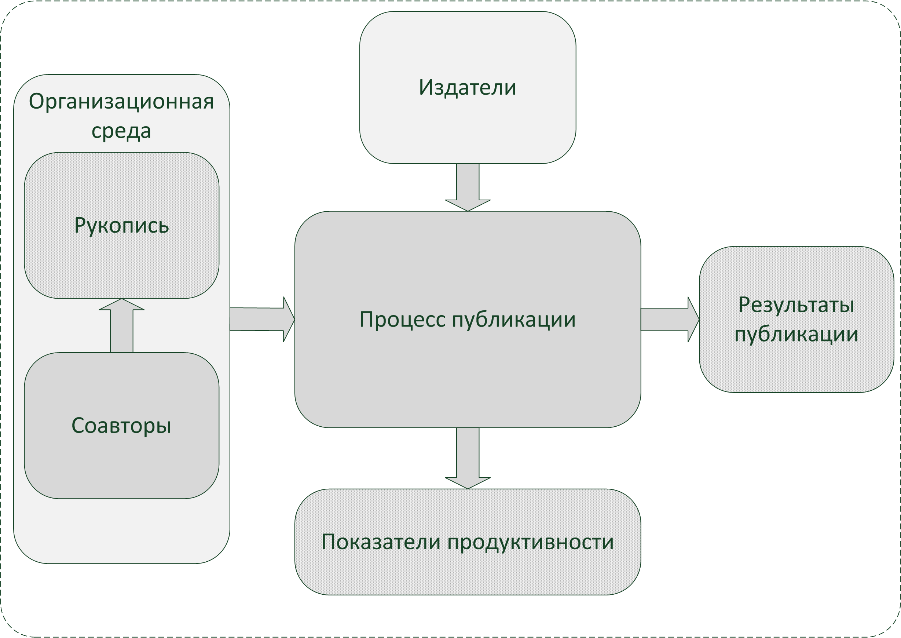
\includegraphics[width=0.8\textwidth]{om1}
  \label{fig:om1}
  \caption{Логический каркас исследования.}
\end{figure}  
Как видно из рисунка, логический каркас исследования включает в себя организационную среду (соавторы и их рукопись), процесс публикации, издателей, показатели продуктивности и результаты публикации.
В следующем подразделе каждый из компонентов логического каркаса будет рассмотрен подробнее.

\subsection{Рукопись}
Как упоминалось ранее, рукопись по форме - это текст.
Методологически рукописи разделяют на следующие основные виды:
\begin{itemize}
\tightlist
\item Монография
\item Научная статья
\item Тезисы доклада
\end{itemize}

Научная статья – это произведение небольшого объема, обычно от 5 до 20 страниц. По содержанию научные статьи разделяются на три типа: 
\begin{itemize}
\tightlist
\item Научно–теоретические статьи
\item Научно–практические статьи
\item Научно–методические статьи
\end{itemize}
Научно–практические статьи посвящены научным экспериментам и реальному опыту. 
Далее будет рассмотрен именно этот тип рукописей.

\subsection{Соавторы}
Большинство исследований выполняют научно-исследовательские коллективы, а не авторы-одиночки. Как следствие, рукописи тоже пишутся в результате коллективного труда. Согласно исследованию \cite{kradoya2016structure}, в нефтегазовой отрасли распределение количества соавторов имеет вид, представленный на рисунке (Рис. \ref{fig:om2}).

\begin{figure}[H]
  \centering
  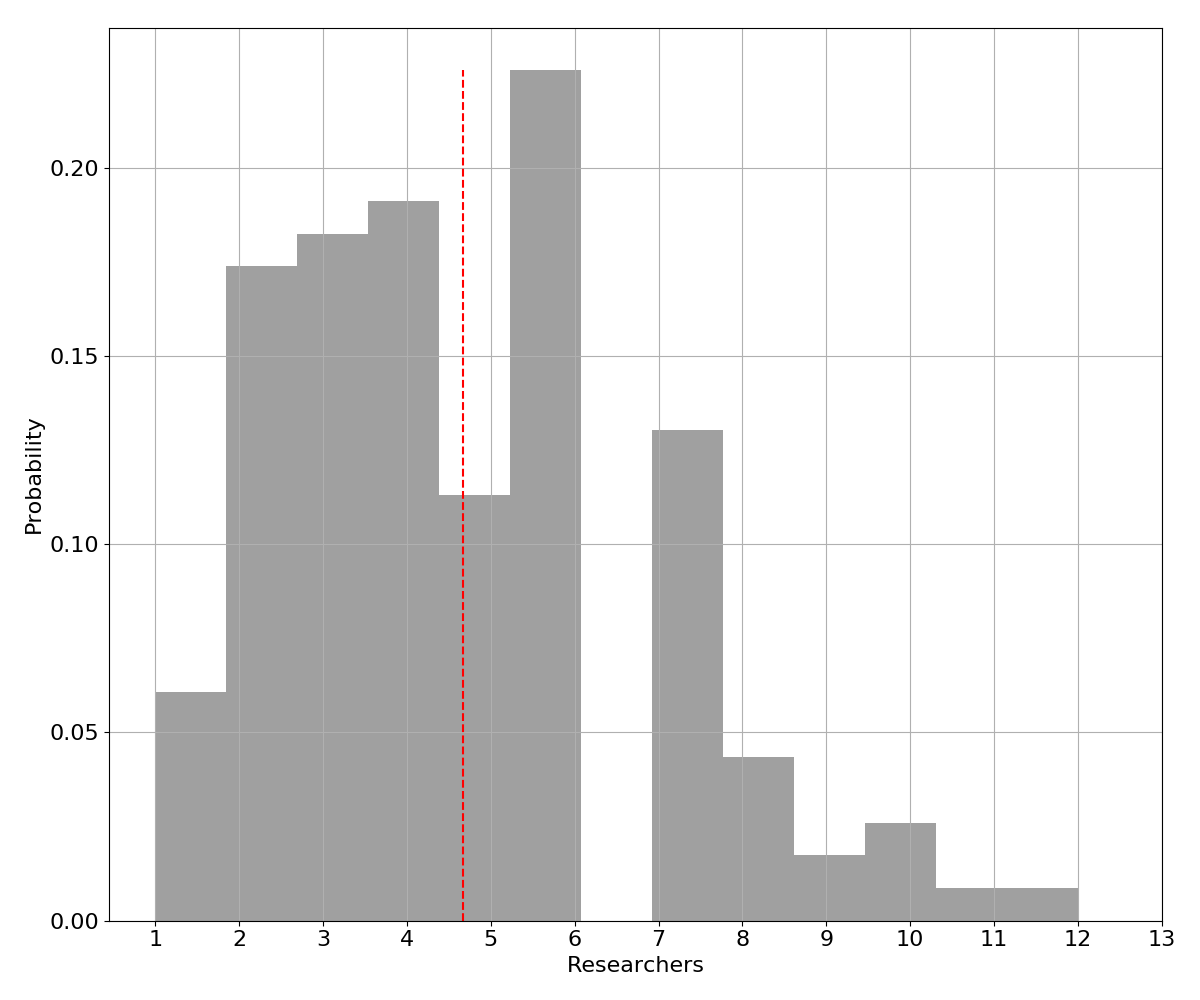
\includegraphics[width=0.8\textwidth]{om2}
  \label{fig:om2}
  \caption{Распределение количества соавторов научных статей в нефтегазовой отрасли. Красной линей обозначено среднее значение: 4.67. Стандартное отклонение распределения равно 2.28.}
\end{figure}  

\subsection{Организационная среда}
Научные исследования проводятся сотрудниками научно-исследовательских подразделений. 
В нефтегазовой отрасли такие подразделений могут принадлежать профильным институтам, научно-техническим центрам, сервисным организациям и другим участникам экосистемы. 
Таким образом, соавторы работают в организационной среде. 
Организационная среда во многом определяет коммуникации между соавторами, что важно на нашего исследования.

\subsection{Процесс публикации}
Процесс публикации состоит из двух типов действий: 
\begin{itemize}
\tightlist
\item Взаимодействие соавторов с издателем
\item Взаимодействие соавторов между собой
\end{itemize}

Объектом обоих действий является рукопись и сопутствующие дополнительные материалы: анкеты, презентации, письма, рецензии.
Основная задача взаимодействий с издателем состоит в удовлетворении условий для публикации статьи в данном издании. 
Обычно требования к авторам обозначены на веб сайтах издателей и могут отличаться.  
Взаимодействия соавторов между собой в процессе публикации включают следующие действия: 
\begin{itemize}
\tightlist
\item Формирование списка возможных издателей
\item Изучение специфики требуемых издателями тематик 
\item Определение временных ограничений на подачу рукописи
\item Составление плана доработок рукописи под требования издателей
\item Сбор сопутствующих документов по требованиям издателей
\item Подготовка презентации для доклада (обязательно для публикации в материалах конференций)
\item Выступление с докладом (командировка)
\item Подтверждение авторства в сообществах ученых и индексах.
\end{itemize}

\subsection{Издатели}
Наиболее значимыми считаются издатели, рекомендованные к публикации Высшей аттестационной комиссией (ВАК). В ``Перечне рецензируемых научных изданий'' ВАК по состоянию на 20.09.2017 содержится 2172 издания. 
Выберем издателей по одной, наиболее близкой для нефтегазовой отрасли специальности — 25.00 ``Науки о земле''. 
Таких изданий оказалось 147 штук. 
Далее автор разработал следующий алгоритм для сбора данных:

\begin{enumerate}
\tightlist
\item Осуществляем поиск веб сайта по названию издания
\item На сайте издания ищем раздел ``Для авторов''
\item Собираем перечень требований к рукописи и заносим в таблицу.
\item Переходим к следующему издателю.
\end{enumerate}

Воспользуемся результатами исследования \cite{mazov2015russian}, чтобы выбрать издателей с наибольшей публикационной активностью и импакт-фактором по международным реферативным базам. 
Список содержит 16 журналов. 
Все 16 журналов имеют общие правила для авторов, разработанные издательством МАИК ``Наука/Интерпериодика''.
Каждое издание имеет свой допустимый объём публикаций, обусловленный количеством статей в одном выпуске и количеством выпусков в год.
Чем больше рукописей поступает к издателю, тем выше конкуренция за право быть опубликованным.  

\subsection{Результаты публикации}
Результатом публикации является определенный вклад в науку. 
Задача максимизации доступности результатов исследования в эпоху Интернет может быть решена с помощью использования интернет ресурсов. 
Приведем лишь некоторые способы для увеличения аудитории: 

\begin{itemize}
\tightlist
\item Международные реферативные базы (Scopus, WoS), 
\item Электронные библиотеки (например, eLibrary.ru),
\item Присвоение научной статье идентификатора цифрового объекта (DOI), 
\item Привязка научной статьи к автору в онлайн сообществах ученых (например, ResearchGate),
\item Публикация статьи в открытых библиотеках (например, arxiv.org),
\item Привязка статьи к идентификационному номеру ученого (например, ORCID, SPIN),
\item Индексы цитирования (например, РИНЦ).
\end{itemize}

Индекс цитирования, например, Российский индекс научного цитирования (РИНЦ), является одним из распространенных наукометрических показателей и применяется для формальной оценки в научных кругах.
Альтернативами индексу цитирования являются экспертная оценка и оценка по импакт-фактору научных журналов.
Углубленные методы библиометрического анализа дают возможность рассмотреть вклад автора с различных точек зрения.
Большое внимание в частности уделяется анализу публикаций с помощью графов соавторства, рассмотренных далее в разделе \ref{sec:coath}. 
Пример графа соавторств приведен на рисунке (Рис. \ref{fig:om3}).

\begin{figure}[H]
  \centering
    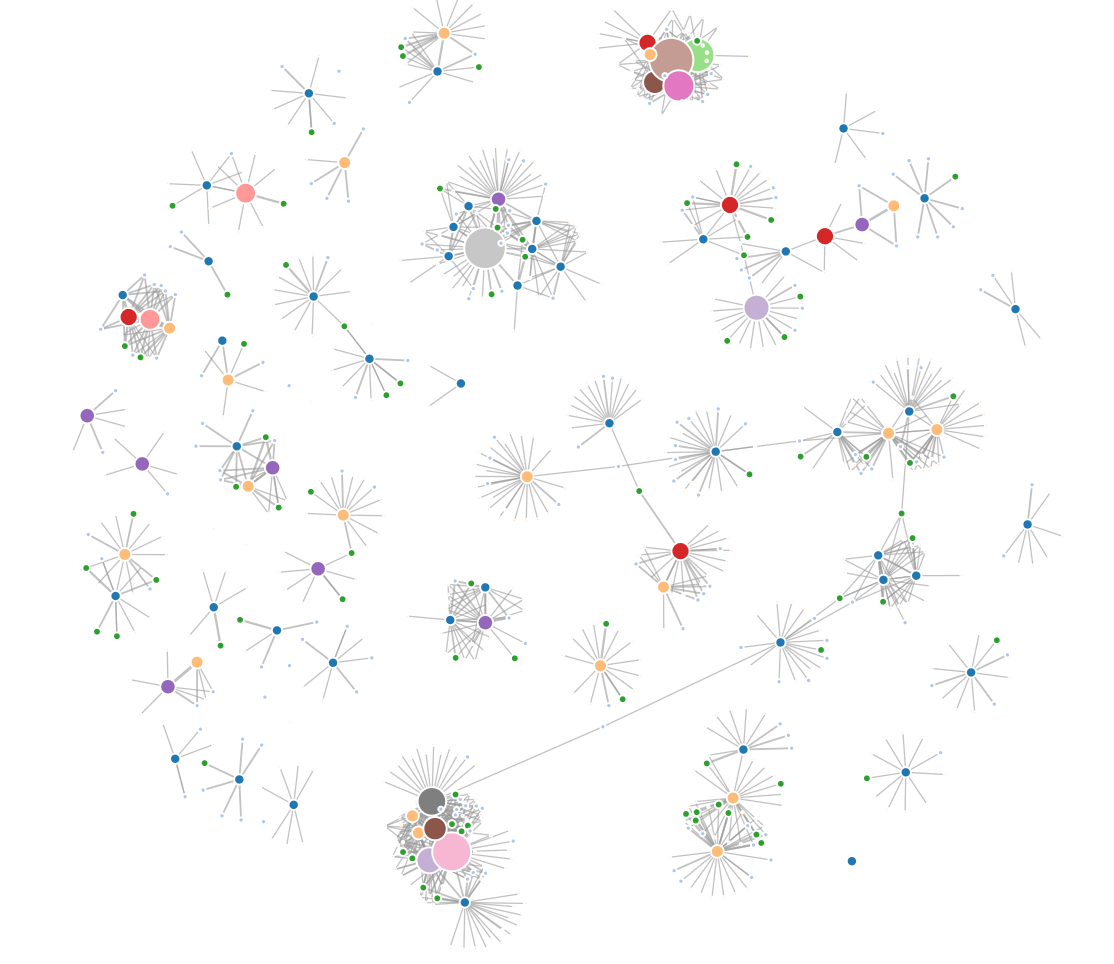
\includegraphics[width=0.8\textwidth]{om3}
  \label{fig:om3}
  \caption{Граф соавторств для ключевого слова \textit{Нефтяные оторочки}}
\end{figure}  

Графы соавторств позволяют визуально выделить наиболее значимых ученых по данной тематике. Например, на рисунке (Рис. \ref{fig:om4}) мы можем видеть такой кластер. 

\begin{figure}[H]
  \centering
    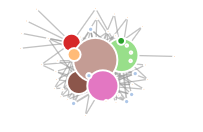
\includegraphics[width=0.2\textwidth]{om4}
  \label{fig:om4}
  \caption{Фрагмент графа соавторства по ключевому слову Нефтяные оторочки. Изображены только узлы, относящийся к профессору Rahim Masoudi.}
\end{figure} 

Принцип построения графов соавторств заключается в отнесении количества публикаций по выбранному ключевому слову к вершинам – авторам, а фактов соавторства к ребрам графа. 
Такой принцип построения графа позволяет анализировать его с помощью методов Анализа социальных сетей (Social network analysis, SNA).

\subsection{Показатели продуктивности публикаций}
Показатели продуктивности процесса публикаций должны давать интегральную характеристику процессу и позволять проводить сравнения различных реализаций процесса. Наиболее полезными представляется показатели, приведенные в таблице (Таб. \ref{tab:om1}):

\begin{table}[H]
\centering
\caption{Показатели продуктивности процесса публикаций}
\label{tab:om1}
\resizebox{\textwidth}{!}{%
\begin{tabular}{ |l|l| }
\hline
\textbf{Название показателя продуктивности} & \textbf{Описание} \\ \hline
Эффективность публикаций & Отношение количества опубликованных рукописей к общему количеству написанных рукописей \\ \hline
Доля опубликованных рукописей на одного автора & Отношение количества опубликованных рукописей к числу авторов \\ \hline
Доля отвергнутых издателями рукописей на одного автора & Отношение количества отвергнутых рукописей к числу авторов \\ \hline
\end{tabular}%
}
\end{table}

Предполагается, что процесс более продуктивен, когда \textit{Эффективность публикаций} стремится к единице, \textit{Доля опубликованных рукописей на одного автора повышается}, а \textit{Доля отвергнутых издателями рукописей на одного автора} стремится к нулю.
Стратегии управления процессом публикации через показатели продуктивности приведены в таблице (Таб. \ref{tab:om2}).

\begin{table}[H]
\centering
\caption{Стратегии управления продуктивностью процесса публикаций через показатели продуктивности.}
\label{tab:om2}
\resizebox{\textwidth}{!}{%
\begin{tabular}{ |l|l|l| }
\hline
\textbf{Название показателя продуктивности} & \textbf{Максимальная продуктивность} & \textbf{Минимальная продуктивность} \\ \hline
Эффективность публикаций & Стремится к единице & Стремится к нулю \\ \hline
Доля опубликованных рукописей на одного автора & Увеличивается & Уменьшается \\ \hline
Доля отвергнутых издателями рукописей на одного автора & Стремится к нулю & Увеличивается \\ \hline
\end{tabular}%
}
\end{table}
Отметим, что приведенные показатели продуктивности никак не характеризуют качество самой научной статьи.
В данном исследовании автор не ставит задачу оценки качества научной работы.

На основании вышеизложенных методических принципов может быть построена модель процесса с помощью системной динамики. 

\section{Теория суррогатного моделирования}

Суррогатная модель лежит в основе нового направления моделирования в инженерии.
Она является математическим методом составления модели, базирующейся на результатах испытаний и/или вычислительных экспериментов, проведенных с разнообразными объектами одного рассматриваемого класса.
В некоторых случаях суррогатное моделирование является единственным способом решения инженерно-технической задачи.

Задачей суррогатного моделирования является оптимизация исходной сложной функции таким образом, чтобы максимально уменьшить область расчета и свести его к минимуму. 
Для упрощения многих инженерных задач строится суррогатная модель целевой функции, которая впоследствии заменяет саму целевую функцию.

Концепция создания суррогатных моделей состоит из следующих этапов: 
\begin{itemize}
\tightlist
\item  
  Характеристика объекта Z, определяющая свойства объекта в некоторых условиях, может быть описана в виде функциональной зависимости $Z= \Phi(X,Y)$,  где переменная X описывает сам объект, а переменная Y задает условия функционирования.
\item
  Функция $\Phi$ является неизвестной, и для ее вычисления проводятся вычислительные эксперименты.
\item
  Имеется некоторое количество измерений $ \Xi = \{ X_i,Y_i,Z_i= \Phi_i ( X_i,Y_i ), i \in \mathbb{R} \} $,
где значение  $Z_i= \Phi_i (X_i,Y_i ) $ характеристики Z получено методом $M_i$ для объекта, имеющего описания $X_i$, в условиях функционирования $Y_i$.
\item
  По известному множеству $\Xi$ с помощью тех или иных математических методов анализа и обработки данных строится функция $\Phi^s (X,Y)$, значение которой принимаются в качестве приближенного значения характеристики Z для объекта с описанием X в условиях функционирования Y.

Если все значения в множестве $\Xi$ получены при помощи одной и той же модели $M$ и $\Phi^s (X,Y) = \Phi^m (X,Y)$, то построенная функция $\Phi^s$ может рассматриваться как ``заменитель'' (суррогат) функции $\Phi^m$.  
\end{itemize}

Суррогатное моделирование успешно применяется в таких областях как электротехника, нефтяное дело, водное хозяйство, военное дело, машиностроение и химическая отрасль.

Незаменимо применение суррогатных моделей и в строительстве для оптимизации аэродинамической формы для выявления оптимальной формы уникальных гражданских сооружений, таких как высотные здания и большепролетные мосты, которые окружены турбулентным потоком.

Следующие задачи нефтегазовой отрасли так же могут быть решены с использованием суррогатных моделей:

\begin{itemize}
\tightlist
\item Построение суррогатных модели резервуара (surrogate reservoir model);
\item Оптимизации расположения скважин;
\item Анализ неопределенности прогноза добычи нефти;
\item Автоадаптация модели резервуара по данным;
\item Задача оптимизации при суперэлементном моделировании разработки нефтяных месторождений.
\end{itemize}

В ряде вычислительных экспериментов для решения задач нефтегазовой отрасли используется вышеописанный мета-алгоритм. 
Например, сначала в гидродинамическом симуляторе производятся расчеты значения функции для определённых узловых значений параметров $X_i$ на основании физических законов движения жидкостей в пористой среде $M_i$, а потом, заданная таким числовым образом функция $\Phi$ используется для получения значений функции $Y_i$  либо на более детализированном множестве значений параметров, либо для значений параметров, выходящих за рамки узловых значений $X_i$.

Одна из основных причин возникновения описанного выше мета-алгоритма построение суррогатной модели заключаются в ограничениях на скорость гидродинамической моделирования. 
В будущем, когда в любое время любой специалист организации сможет варьировать значения параметров в широком диапазоне и в режиме близком к реальному времени получать искомые значения функции потребность в суррогатных моделях скорее всего отпадет.
А пока моделирование производится на дорогостоящих высокопроизводительных кластерах, специалистами за времена, измеряемые в часах, а иногда и днях для одного набора параметров существует потребность в прозорливой подготовке данных которые могут понадобиться в дальнейшем.
Так как, потребность в изменении параметров может возникать по несколько раз в день и у самых разных специалистов различных подразделений организации, то применение суррогатного моделирования является насущной необходимостью.
Получаемая суррогатная модель $\Phi^s$, иногда ее называют прокси-моделью, превосходит изначальную модель $\Phi^m$ по вычислительной силе во много раз, то есть, не требует большого объема вычислительных ресурсов и работает в режиме близком к реальному времени.

\section{Непараметрические модели}
Для того, чтобы понять, что такое непараметрические модели рассмотрим параметрические модели. 
Параметрической модель $p$ для значений $y$, зависящих от переменных $X$  и параметров $\theta$  будет иметь вид  $p \left( y\vert	,\theta \right)$.
Нахождение  параметров $\theta$ с помощью методов максимизации апостериорной вероятности $p \left( \theta \vert y,X \right)  \longrightarrow \max_\theta $.

Для поиска оптимальных параметров математической модели используются методы оптимизации.

Численные методы оптимизации:

\begin{itemize}
\tightlist
\item  Градиентные и безградиентные, 
\item  Одно и много критериальные, 
\item  Робастные (для задач оптимизации в условиях неопределенности), 
\item  Основанные на суррогатных моделях (surrogate -- based),
\end{itemize}

Рассмотрим методы Байесовской оптимизации, которые наиболее часто применяются в суррогатном и имитационном моделировании. 
При этом данные и модель являются ``черным ящиком''.

Пусть дана функция  $ f \left(  x \right)$  и нам нужно найти $x$ при котором она достигает максимума  $ f \left(  x \right) \longrightarrow \max_x$. Добавим условие при котором расчет каждого значения  $ f \left(  x \right)$ это ресурсоемкая задача. Такое условие встречается в следующих случаях: 

\begin{itemize}
\item $x$ - это географические координаты скважины, а  $ f \left(  x \right)$ -- это количество нефти, которое можно добыть, пробурив скважину с координатами $x$. В таком случае одно значение  $ f \left(  x \right)$ стоит миллионы рублей;
\item $x$ - это гиперпараметры искусственной нейронной сети глубокого обучения,  $ f \left(  x \right)$  -- это целевая метрика точности предсказания. В этом случае одно значение  $ f \left(  x \right)$ будет занимать месяцы работы;
\item $x$ - это лекарство, а  $ f \left(  x \right)$ - эффективность лекарства против болезни. В таком случае одно значение  $ f \left(  x \right)$ будет стоить жизни одного подопытного животного.
\end{itemize}

Таким образом, постановка задачи состоит в том, чтобы оптимизировать целевую функцию за минимальное количество попыток.
При этом использование суррогатных моделей целевой функции позволяет сделать каждый шаг оптимизации менее ресурсоемким. 
Введем функцию ценности обнаружения  $ \mu \left(  x \right)$, которая характеризует выгоду полученную от оптимизации  $ f \left(  x \right)$ при использовании суррогатной модели $\hat{f}$.
Функция ценности обнаружение является количественной оценочной функцией для минимализации количества попыток. 
Расмотрим следующие  $ \mu \left(  x \right)$:

\begin{itemize}
\item Maximum probability of improvement (MPI): $ \mu \left( x \right) = P(\hat{ f} \left( x  \right) \geq f^* + \epsilon =  \Phi \bigg( \frac{\mathbb{E}\hat{ f} \left( x  \right) - f^* -\epsilon}{Var[\hat{ f } \left( x  \right)]}\bigg) $, где $f^*$ - текущее лучшее значение.
\item Upper confidence bound (UCB): $  \mu \left(   x \right) = \mathbb{E}\hat{ f } \left( x  \right) + \eta Var[\hat{ f} \left( x  \right)] $
\item Expected improvement (EI): $  \mu \left(   x \right) = \mathbb{E} \max( f \left( x  \right) - f^*,0)  = Var[\hat( f \left( x  \right)] \cdot [z \Phi (z) + \phi(z)]$, где $z = \frac{\mathbb{E}\hat{ f }\left( x  \right) - m\left( x \right)}{Var[\hat{ f } \left( x  \right)]}$
\item 
\end{itemize}

\section {Байесовские методы для определения параметров НТЦ}

Рассмотрим результаты деятельности НТЦ как наблюдения $x$, тогда в самом общем смысле в качестве задачи поставим найти распределение случайной величины $\theta$, приводящей к имеющимся наблюдениям.

Согласно теореме Байеса имеем выражение \ref{eq:bay}.

\begin{equation} \label{eq:bay}
p \left(  \theta \vert x \right) = \frac{p \left ( x \vert \theta \right) \, p \left(  \theta \right)} {\sum_i p \left(  x \vert \theta_i \right) \, p \left(  \theta_i \right)}
\end{equation}

Для вычисления апостериорного распределения $p \left(  \theta \vert x \right)$ на основании функции правдоподобия $p \left ( x \vert \theta \right)$, априорного распределения с плотностью вероятности $p \left(  \theta_i \right)$ и полной вероятностью $p \left(  x \right) = \sum_i  p \left(  x \vert \theta_i \right) p \left(  \theta_i \right)$. 

Вычисление полной вероятности $p \left(  x \right)$ является сложной задачай, поэтому воспользуемся принципом максимизации апостериорной вероятности $p \left( \theta \vert  x \right)$. Найдем такие параметры $\theta_{MAP}$ при которых выражение $p \left( \theta \vert  x \right)$ максимально. Принцип максимализации апостериорной вероятности (Maximum A Posteriori, MAP) можно записать в виде: 
\begin{eqnarray*} 
\theta_{MAP} & = & \operatorname*{arg\,max}_\theta p \left( \theta \vert  x \right)\\
			 & = & \operatorname*{arg\,max}_\theta \frac{p \left( x \vert \theta \right) \, p \left( \theta \right)} {p \left(  x \right)}
\end{eqnarray*}

Так как полная вероятность $p \left(  x \right)$ не зависит от $\theta$, то можем убрать знаменатель и получить формулировку для оптимизационной проблемы в виде:
\begin{equation} \label{eq:mpopt}
\theta_{MAP} = \operatorname*{arg\,max}_\theta p \left( x \vert \theta \right) p \left( \theta \right)
\end{equation}

Уравнение ~\ref{eq:mpopt} не содержит $p \left(  x \right)$ и может быть решено с помощью численных методов. Но данный подход страдает от следующих проблем: 
\begin{itemize}
	\item Нет инвариантности относительно параметров распределения $\theta_{MAP}$;
	\item $\theta_{MAP}$ не применима в качестве априорного распределения;
	\item Нет возможности оценить байесовский достоверный интервал (credible interval).
\end{itemize}

Рассмотрим частный случай $\theta_{MAP}$ когда вероятности всех $\theta$ одинаковы - юниформное распределение. 
Тогда задача поиска $\theta$ сводится к поиску максимального значения для $p \left( x \vert \theta \right)$. 
Такой подход называют методом оценки максимального правдоподобия (maximum likelihood estimation, MLE).
Запишем выражение оптимизационной задачи для метода оценки максимального правдоподобия.

\begin{equation} \label{eq:mle0}
\theta_{MLE} = \operatorname*{arg\,max}_\theta p \left( x \vert \theta \right) = \operatorname*{arg\,max}_\theta \prod_i p \left( x_i \vert \theta \right)
\end{equation}

Без потери общности можем максимизировать логарифм от правой части выражения ~\ref{eq:mle0}.

\begin{equation} \label{eq:mle1}
\theta_{MLE} = \operatorname*{arg\,max}_\theta \log p \left(  x \vert \theta \right) 
\end{equation}

\begin{eqnarray*} \label{eq:mle2}
\theta_{MLE} & = & \operatorname*{arg\,max}_\theta \log \prod_i p \left( x_i \vert \theta \right) \\
             & = & \operatorname*{arg\,max}_\theta \sum_i \log p \left( x_i \vert \theta \right)
\end{eqnarray*}

Покажем подробнее как MAP преобразуется в MLE для случая юниформного распределения $\theta$:
\begin{eqnarray*} \label{eq:mapmle}
\theta_{MAP} & = &\operatorname*{arg\,max}_\theta \sum_i \log p \left( x_i \vert \theta \right) p \left( \theta \right) \\
             & = & \operatorname*{arg\,max}_\theta \sum_i \log p \left( x_i \vert \theta \right) \, const \\
             & = & \operatorname*{arg\,max}_\theta \sum_i \log p \left( x_i \vert \theta \right) \\
             & = & \theta_{MLE}
\end{eqnarray*}

Еще одним подходом к оценке $\theta$  является метод сопряжённых априорных распределений. 
В теореме Байеса ~\ref{eq:bay} изменяемым является только член $p \left( \theta \right)$, так как функция правдоподобия $p \left( x \vert \theta \right)$ определяется моделью, а $p \left(  x \right)$  данными.

Распределение априорной вероятности называется сопряженным с распределением постериорной вероятности, если они относятся к одному семейству распределений. 

Поясним вышеизложенное на примере. 
Пусть $p \left( x \vert \theta \right)$  и $p \left( \theta \right)$ являются нормальными распределениями.
Для распределения $p \left( \theta \right) = N(x \vert \mu_0,\sigma_0^2)$  с математическим ожиданием $\mu_0$ и дисперсией $\sigma_0^2$ выражение ~\ref{eq:bay} может быть записанно в виде ~\ref{eq:bayconj}.

\begin{equation} \label{eq:bayconj}
p \left( \theta \vert  x \right) = \frac{\mathbb{N}(x \vert \theta ) \, \mathbb{N}(\theta \vert \mu_0 , \sigma_0^2)} {p \left(  x \right)}
\end{equation}

Произведение двух нормальных распределений будет так же нормальным распределением, и параметры постериорного распределения можно будет вычислить по следующим формулам.
\begin{eqnarray}
\label{eq:bayconj1}
\mu & = & \frac{\left( \frac{\mu_0}{\sigma_0^2} + \frac{\sum_{i=1}^n x_i}{\sigma^2}\right)} { \frac{1}{\sigma_0^2}+ \frac{n}{\sigma^2} }\\
\sigma & = & \left( \frac{1}{\sigma_0^2} + \frac{n}{\sigma^2}\right)^{-1}
\end{eqnarray}

Таким образом использование сопряжённых семейств распределений позволяет избежать сложных вычислений полной вероятности.

\subsection{Скрытые параметры модели}
Говоря о характеристиках НТЦ, как объекта исследования мы не можем измерить такие параметры как интеллектуальный капитал (ИК).
Хотя ИК влияет на результаты деятельности НТЦ, которые мы можем измерить, например, на  количество публикаций и количество авторов.
Будем называть такие параметры как ИК скрытыми параметрами.

Для определения ИК можно рассмотреть подход на основании машинного обучения. 
Например, на основе искусственной нейронной сети. 
Тогда нам для обучения искусственной нейронной сети будет необходим набор данных, содержащий значения ИК для различных компаний с разными параметрами: количеством публикаций, количеством сотрудников, и.т.п.
Из литературы известно, что для обучения искусственных  нейронных сетей необходимы наборы данных с сотнями тысяч образцов и сотнями параметров.  
В действительности такого набора данных для НТЦ не существует. 
Но даже есть представить, что такой набор данных есть, то он будет содержать много пропущенных значений, противоречивых данных и других проблемных данных.

С другой стороны, Байесовская статистика может работать с небольшими наборами данных. 
Что приводит нас к рассмотрению вероятностного подхода к оценке скрытых параметров. 
Первым шагом для построений вероятностной модели является построение зависимости наблюдаемых параметров. И на первый взгляд все параметры будут зависит друг от друга. 
Например, чем больше авторов, тем больше публикаций, чем больше сотрудников с учеными степенями, тем больше публикаций в журналах из списка ВАК и т.п. 

%%Нужна картинка с картой связей без ИК. Каждый с каждым.

Но такая полносвязанная структура модели не позволяет нам построить структурированную вероятностную модель, так как нам необходимо будет оценить вероятность каждой возможной комбинации параметров.
А количество таких комбинаций будет экспоненциально расти с количеством рассматриваемых параметров.  

%%Нужна картинка с картой связей с ИК.
%% Bayesian network

Одним и решений может быть введение скрытых параметров, таких как ИК, которые уменьшают количество связей. 
Предположим, что НТЦ обладает ИК от которого зависит число публикаций и количество авторов. 
Таким образом, количество комбинаций для вероятностной оценки существенно сокращается.


\subsection{EM-алгоритм}
Рассмотрим вероятностную формулировку неравенства Йенсена. 
Пусть $(\Omega,\mathcal{F},\mathbb{P})$ — вероятностное пространство, и $X\colon\Omega \to \mathbb{R}$ — определённая на нём случайная величина. 
Пусть также $\varphi\colon\mathbb{R} \to \mathbb{R}$ — выпуклая (вниз) функция. 
Тогда, если $X, \varphi(X) \in L^1(\Omega,\mathcal{F},\mathbb{P})$, то  $\varphi(\mathbb{E}[X]) \leqslant \mathbb{E}[\varphi(X)]$, где $\mathbb{E}[\cdot]$ означает математическое ожидание. 
Или другими словами для выпуклой функции $f$ и распределения вероятностей $t$ получаем следующее выражение \ref{eq:jen}: 

\begin{equation} \label{eq:jen}
f (\mathbb{E}_{p \left( t \right)} \, t) \geqslant \mathbb{E}_{p \left( t \right)}f(t)
\end{equation}

Для дальнейшего рассмотрения приведем следующее определение расстояния Кульбака — Лейблера \ref{eq:kl0}. 

\begin{equation} \label{eq:kl0}
\mathcal{KL}(q \Vert  p) = \int_x q \left( x \right) \, \log \frac{q \left( x \right)}{p \left(  x \right)} \, {\rm d}x
\end{equation}

Отметим, что точнее будет называть расстояния Кульбака — Лейблера мерой различия двух распределений $q \left( x \right)$ и $p \left(  x \right)$, так как по определению данная мера не обладаем симметрией: $\mathcal{KL}(q \Vert p) \neq \mathcal{KL}(p \Vert q)$. 

Покажем еще одно полезное свойство расстояния Кульбака — Лейблера: $\mathcal{KL}(q \Vert p) \geqslant 0$.
Для этого произведем следующие вкладки:
\begin{eqnarray}\label{eq:kl03}
\mathcal{KL}(q \Vert   p) 
& = & \mathit{E}_q \left(  - \log	 \frac{q}{p} \right) \\
& = & \mathit{E}_q \left(  - \log	 \frac{p}{q} \right) \leqslant  \log \left( \mathit{E}_q \frac{q}{p} \right)\\
& = & \log \int_x q \left( x \right) \, \frac{q \left( x \right)}{p \left(  x \right)} \, {\rm d}x \\
& = & 0
\end{eqnarray}
Рассмотрим применение EM-алгоритма для нахождения скрытых параметров НТЦ.
Предположим, что у на есть модель НТЦ со скрытыми параметрами. 
Обозначим скрытые параметры как $t_i$, а наблюдаемые параметры как $x_i$. 
Тогда функцию правдоподобия можно выразить как ~\ref{eq:em0}.
\begin{equation} \label{eq:em0}
p \left( x_i \vert	\theta \right) = \sum_c p \left( x_i \vert t_i = c \right) p \left( t_i = c \vert \theta \right) 
\end{equation}

Где $p \left( t_i = c \vert \theta \right)$  - это априорная вероятность того, что $t$ принимает значение $t$. 
Задача состоит в том, чтобы максимизировать вероятность функции правдоподобия по $\theta$. 
Так как логарифм является выпуклой непрерывно возрастающей функцией, то будем искать максимум логарифма от $p \left( x_i \vert	\theta \right)$. 
Предположим так же, что все $N$ измерений $x_i$ были сделаны независимо. 
Тогда вероятность $X = \prod_i^N p \left( x_ \vert \theta \right) $

\begin{equation} \label{eq:em1}
\log p \left(  X \vert	\theta \right) = \sum_i^N \log p \left( x_i \vert \theta \right) = \sum_i^N \log \sum_c p \left(  x_i \vert t_i = c \vert \theta \right)
\end{equation}
Стоит отметить, что мы можем искать максимум выражения ~\ref{eq:em1}  с помощью градиентных методов. 
Например, с помощью метода стохастического градиентного спуска. 
Но автор сознательно применил другой алгоритм и покажет его преимущества далее.

Применим неравенства Йенсена ~\ref{eq:jen} к выражению ~\ref{eq:em1} и получим $\log p \left(  X \vert	\theta \right) \geqslant \mathfrak{L}(\theta, q)$.  
Далее выберем функцию $\mathfrak{L}(\theta, q)$ так, чтобы ее легко было максимизировать.
\begin{equation} \label{eq:em2}
\mathfrak{L}(\theta, q) = \sum_i^N \sum_c q(t_i = c) \log \frac{p \left( x_i, t_i = c \vert \theta \right)}{q(t_i = c)}
\end{equation}
И в итоге для параметра $\theta$ и распределения $q$ получим неравенство ~\ref{eq:em3}:
\begin{equation} \label{eq:em3}
\log p \left(  X \vert	\theta \right) \geqslant \mathfrak{L}(\theta, q)
\end{equation}
Теперь для поиска максимума $mathfrak{L}(\theta, q)$  применим  следующий итерационный алгоритм из двух шагов для каждой итерации $k$:

\begin{itemize}
	\item Фиксируем $\theta^k$ и выбираем $q^k$ так чтобы $\mathfrak{L}(\theta^k, q^k)$ была максимальной
	\item Получаем $q^{k+1} = \operatorname*{arg\,max}_q \mathfrak{L}(\theta^k, q)$
\end{itemize}

Первый шаг принято называть E-шаг, а второй M-шаг. Вместе они представляют EM-алгоритм результатом, которого является $\theta$ для скрытой переменной $t$. 

\subsection{E-шаг}
Рассмотрим более подробно E-шаг. 
Максимизация функции нижней границы $\mathfrak{L}(\theta^k, q^k)$ означает, что расстояние между $\mathfrak{L}(\theta^k, q^k)$ и функцией максимального правдоподобия $\log p \left(  X \vert	\theta^k \right)$. 
Запишем это уравнение для k-й итерации и покажем, что это расстояние можно выразить через расстояния Кульбака — Лейблера.
\begin{eqnarray*} \label{eq:em4}
DIST & = & \log p \left( X \vert \theta \right) - mathfrak{L}(\theta, q) \\
       & = & \sum_i^N \log p \left( x_i,\theta \right) - \sum_i^N \sum_c q(t_i = c) \log \frac{p \left( x_i,t_i=c \vert \theta \right)}{q(t_i=c)} \\
       & = & \sum_i^N  \big\{ \log p \left( x_i \vert \theta \right) \sum_c q(t_i=c) - \sum_c q(t_i = c) \log \frac{p \left( x_i,t_i=c \vert \theta \right)}{q(t_i=c)} \big\} \\
       & = & \sum_i^N \sum_c q(t_i = c) \big\{ \log p \left( x_i \vert \theta \right) - \log \frac{p \left( x_i,t_i=c \vert \theta \right)}{q(t_i=c)} \big\} \\
       & = & \sum_i^N \sum_c q(t_i = c) \big\{ \log p \left( x_i \vert \theta \right) - \log \frac{p \left( x_i,t_i=c \vert \theta \right)}{q(t_i=c)} \big\} \\
       & = & \sum_i^N \sum_c q(t_i = c) \log  \frac{p \left( x_i \vert \theta \right) q(t_i=c)}{p \left( x_i,t_i=c \vert \theta \right)}  \\
       & = & \sum_i^N \sum_c q(t_i = c) \log  \frac{p \left( x_i \vert \theta \right) q(t_i=c)}{p \left( t_i \vert x_i,\theta \right) p \left( x_i \vert \theta \right)}  \\
       & = & \sum_i^N \sum_c q(t_i = c) \log  \frac{ q(t_i=c)}{p \left( t_i \vert x_i,\theta \right) }  \\
       & = & \sum_i^N \mathcal{KL}( q(t_i)  \Vert   p \left( t_i \vert x_i, \theta \right) )\\
\end{eqnarray*}

Таким образом, максимизация функции нижней границы $\mathfrak{L}(\theta^k, q^k)$ эквивалентна минимизации суммы расстояний Кульбака — Лейблера для $q(t)$ и $p \left( t \vert x, \theta \right)$. 
Так как расстояния Кульбака — Лейблера неотрицательны по определению, то мы можем приравнять их нулю для поиска глобального минимума.
\begin{equation} \label{eq:em5}
0 = \sum_i^N \mathcal{KL}( q(t_i)  \Vert   p \left( t_i \vert x_i, \theta \right) ) 
\end{equation}

Также из определения расстояния Кульбака — Лейблера известно, оно равно нулю только в случае если оба распределения совпадают. 
\begin{equation} \label{eq:em6}
 q(t_i)  =  p \left( t_i \vert x_i, \theta \right) 
\end{equation}
Уравнение ~\ref{eq:em6}  означает, что для нахождения оптимального распределения $q(t)$ мы должны выбрать его равным постериорному распределению $p \left( t \vert x,\theta \right)$.

\subsection{М-шаг}
На М-шаге производится максимизация функции правдоподобия ~\ref{eq:em2} при фиксированном $q(t)$ по $\theta$.
\begin{eqnarray*} \label{eq:em7}
\mathfrak{L}(\theta, q) & = &  \sum_i^N \sum_c q(t_i = c) \log \frac{p \left( x_i, t_i = c \vert \theta \right)}{q(t_i = c)} \\
& = &  \sum_i^N \sum_c q(t_i = c) \log p \left( x_i, t_i = c \vert \theta \right) - \sum_i^N \sum_c q(t_i = c) \log {q(t_i = c)} 
\end{eqnarray*}

Отметим, что так как выражение $\sum_i^N \sum_c q(t_i = c) \log  {q(t_i = c)}$ не зависит от $\theta$, то при дифференцировании оно обнулится. 
Таким образом, выражение ~\ref{eq:em7}  можно преобразовать следующим образом.
\begin{equation} \label{eq:em8}
\mathfrak{L}(\theta, q)  = \mathbb{E}_{q}\log p \left( X,T \vert \theta \right) + const
\end{equation}

Напомним, что в выражении ~\ref{eq:em8} $X$ - это все данные, а $T$ - это все значения скрытых переменных. $\mathbb{E}_{q}$ обозначает математическое ожидание распределения $q$. Так как мы выбираем распределения для $X$ и $T$, то в наших силах обеспечить чтобы $ p \left( X,T \vert \theta \right)$ была гладкой и непрерывной. Такой выбор значительно упростит нахождения экстремума по $\theta$.

\subsection{Сходимость ЕМ-алгоритма}
ЕМ-алгоритм предназначен для нахождения локальных экстремумов функции максимального правдоподобия. 
Для этого используется функция нижней границы $\mathfrak{L}(\theta^k, q^k)$, которая в процессе оптимизации не убывает ~\ref{eq:em9}. 
\begin{equation} \label{eq:em9}
\log p (X \vert  \theta ^{k+1} ) \geqslant \log p (X \vert  \theta ^{k} )
\end{equation}

\subsection{Использование ЕМ-алгоритма для выявления скрытых тематик в тексте}
Научный текст является одним из проявлений деятельности НТЦ. 
Выявление тематик текста может быть сделано с использованием распределения Дирихле. 
Байесовская модель для постериорного распределения скрытых тематик в тексте может быть записана в следующем виде.

\begin{eqnarray*} \label{eq:lda1}
p \left( W,Z,\Theta \right) = \prod_{d=1}^{D} p \left( \theta_d \right) \prod_{n=1}^{N_d} p \left( z_{dn} \vert \theta_d \right) p \left( w_{dn} \vert z_{dn} \right) \\
p \left( \theta_d \right) \sim Dir( \alpha ) \\
p \left( z_{dn} \vert \theta_d \right) = \theta_{dz_{dn}} \\
p \left( w_{dn} \vert z_{dn} \right) = \Phi_{z_{dn}w_{dn}} \\
\sum_w \Phi_{tw} = 1 \\
\Phi_{tw} \geqslant 0
\end{eqnarray*}

Таким образом, что $W$ - это текстовые данные (научные статьи, документы),  $\Phi$ - распределение слов в каждой тематике, $Z$ - распределение тематик для каждого слова, $\Theta$ - распределение тематик в документе.
Оптимизационная задача для поиска тематик выглядит следующим образом: 
\begin{equation} \label{eq:lda2}
P(W \vert \Phi) \rightarrow max_\Phi
\end{equation}

Для использования ЕМ-алгоритма выпишем явно уравнения для Е-шага и М-шага:

Е-шаг:
\begin{equation}\label{eq:lda3}
\mathcal{KL} (q(\Theta) \, q(Z)  \Vert   p \left( \Theta,Z \vert W \right) ) \rightarrow \underset{q(\Theta) \, q(Z)} {\text{minimize}}
\end{equation}

М-шаг:
\begin{equation}\label{eq:lda4}
\mathbb{E}_{q(\Theta) \, q(Z)} \log p \left( \Theta,Z,W \right) \rightarrow \underset{\Phi}{\text{maximize}}
\end{equation}

Полученные выражения для Е-шага (\ref{eq:lda3}) и М-шага (\ref{eq:lda4}) позволяют получить скрытые тематики их текста. 

\section{Моделирование самоорганизующихся команд в научной среде}

Самоорганизация рабочих групп представляет большой интерес для научно-технических организаций, ищущих новые формы эффективной организации труда сотрудников.
Рассмотрение феномена самоорганизации, как альтернативы формированию рабочих групп привело к построению модели процесса самоорганизации. 
Рассмотрение жизненного цикла рабочей группы по отношению к поставленной цели позволило ввести формальные критерии оценки эффективности работы группы и прогнозировать ее продуктивность.

Важным фактором, влияющим на продуктивности рабочей группы, является характер решаемой задачи. 
Автор предложил собственную классификацию творческих задач нефтегазовой отрасли на основании компетенций, необходимых для их решения. 

В рамках разработанной методики жизненного цикла рабочей группы и классификации задач была построена математическая модель самоорганизации рабочих групп для решения творческих задач. Калибровка математической модели появления рабочих групп была проведена на данных Газпромнефть НТЦ. 

В созданной системе показателей эффективности был проведен цифровой имитационный эксперимент для выявления основных характеристик самоорганизации рабочих групп.

В результате была сделана кластеризация творческих задач по эффективности решения различными рабочими группами, составлены рекомендации по созданию организационных мероприятий, способствующих повышению вероятности самоорганизации рабочих групп, выделены критерии отнесения творческих задач к различным типам рабочих групп, определены основные критерии для формирования эффективных рабочих групп.

Моделирование групповых действий индивидуумов зависит от потенциальных участников группы и целей. 
Например, фанаты футбольного клуба легко объединяются в группу, но не имеют конкретной цели. 
С другой стороны, ученые могут объединяться в исследовательскую группу для конкретной цели, например, написания научной статьи. 
Одинаковы ли принципы объединения в этих случаях? 

Разделяют два процесса появления групп:
\begin{enumerate}
\item Самоорганизация – процесс упорядочения сотрудников за счёт внутренних факторов, без внешнего специфического воздействия, 
\item Формирование – назначение участников группы из вне.
\end{enumerate}

Пример формирования группы в организационной среде: 

\textit{Начальник управления принимает решение сформировать рабочую группу для создания системы разработки месторождения из двух разработчиков месторождений}. 

Пример самоорганизации группы в организационной среде: 

\textit{Несколько разработчиков месторождений решили, что им вместе нужно усовершенствовать методы обработки данных о технических режимах работы скважин с помощью методов машинного обучения и самозабвенно работают в вместе по выходным над этой задачей.
} \label{exp:2}

Решение о создании группы внутри ведет к самоорганизации, решение о создании группы из вне формирует группу. 
Отметим, что на практике процесс появления рабочих групп представляет суперпозицию самоорганизации и формирования. 
Но для исследовательских целей в данной работе авторы намерено рассматривают формирование и самоорганизацию раздельно для выявления родовых признаков этих явлений.

Группа создается на определенное время и для решения конкретной задачи. 
В этом смысле на лицо признаки проектной деятельности – уникальность результата и ограниченность ресурсов для достижения поставленной цели. 
Таким образом, обоснованным представляется применять проектную методику оценки эффективности группы, как проектной команды. 

Структура группы определяется характером решаемых задач. 
Для задач массового обслуживания, например, в рабочие группы в центрах обработки вызовов объединяют специалистов с определенным, одинаковым профилем компетенций. 
Разделение обязанностей в такой группе почти нет: типовые задачи по обслуживанию требуют стандартизованных действий членов группы.
Нагрузка равномерно распределяются по членам группы.

Группа, созданная для решения творческой задачи менее однородна. 
Для решения творческой задачи необходимы специалисты с разными компетенциями. 
Образно можно представить, как задача декомпозируется на компетенции участников.
И это не равномерное распределение, участникам достаются разные объемы работы в рамках их компетенций. 
Для приведенного выше примера (Пример  \ref{exp:2}), задача требует компетенций в технических режимах работы скважин и методах машинного обучения. 
Что будет, если компетенций нужных для достижения цели нужно больше, чем есть у группы? 
Каждый из участников группы выполнит работы в рамках своих компетенций, но цель не будет достигнута, так как останутся невыполненные работы. 
Это распространенная ситуация, как при неправильном планировании групп (формировании), так и при самоорганизации групп. 
Результат работы в такой ситуации оказывается отрицательным, но отношение к этому результату разное в случае самоорганизации и формирования.

Основными критериями эффективности рабочих групп является результат их деятельности и сроки достижения этого результата – это общепринятые организационные показатели эффективности.
Исследование феномена самоорганизации рабочих групп в динамике является сложнейшей организационной задачей. 
Поэтому автор использовал в данной работе математическую модель феномена самоорганизации рабочих групп. 
Математическая модель дает возможность изучить наиболее характерные аспекты феномена самоорганизации, но обладает определённой степенью приближения, неточности. 
Вычислительный эксперимент на основании созданной модели самоорганизации рабочих групп, который представлен далее состоит в том, чтобы оценить результаты работы различных групп над различными задачами. 
В связи с такой постановкой эксперимента возникают следующие исследовательские вопросы: 
\begin{enumerate}
\item Как происходит самоорганизация групп? Какие сотрудники могут самоорганизоваться, а какие нет? Как на самоорганизацию влияют компетенции, опыт, социальные факторы?
\item Какие организационные условия необходимы для самоорганизации групп в научно-технической среде? Конкурсы? Обучения? Мероприятия? 
\item С каким типом задач самоорганизованные группы справляются эффективнее, чем сформированные? 
\item Каковы принципы формирования групп для наиболее эффективного решения творческих задач? 
\end{enumerate}

Оценке эффективности научно-исследовательских и опытно-конструкторских проектов, а также исследованию факторов, влияющих на результативность научной деятельности посвящены многочисленные публикации, см., например, \cite{shcherb1982,ovch2009,fursov2016,shmatko2017}.
Как правило, в этих работах научный коллектив рассматривается как ``чёрный ящик'', производящий научные результаты, и оценка его эффективности производится только на основе выпускаемых результатов, внутренняя структура исследовательской группы обычно не берется в учёт. 
Самоорганизующиеся команды подробно изучены в работе \cite{moe2008understanding}.  
Отдельно исследуются мотивирующие факторы \cite{shmatko2017} и факторы, влияющие на результативность \cite{fursov2016}.

При этом тема моделирования и анализа командной работы также является хорошо проработанной и активно исследуется с середины XX века, см. \cite{bavelas1948mathematical,nov2008,bei2014}. 
Формальное описание профиля компетенций --- это тема многочисленных исследований и публикаций, см., например, \cite{rozewski2009competence,bei2014}.

Первым приближением может быть модель ограниченная существованием фиксированного набора определенных навыков. 
При этом профиль компетенции каждого сотрудника можно описать в виде вектора значений, в котором каждая координата описывает уровень его владения соответствующим навыком.

Вектор, описывающий профиль компетенций команды, получается в результате простого сложения профилей компетенций участников. 
Такая модель естественно возникает, если измерять уровень компетенции производительностью при выполнении соответствующего типа задач. 
Тогда естественно предполагать, что при совместной работе в команде производительность участников складывается.

Аналогичным вектором можно также описать и профиль задачи.
Для подготовки и проведения научного исследования с учетом ограничения по времени требуется определенный уровень производительности для каждого типа задач.

В данной работе рассматриваются самоорганизующиеся малые команды, в которых инициатива создания исходит от сотрудников. 
Это допущение соответствует реальной ситуации в большинстве научных коллективов, где администрация может различными способами мотивировать сотрудников подать заявку на участие в той или иной научной конференции или рекомендовать подготовить статью для определенного журнала, но итоговое решение, как правило, остается за научным сотрудником.

В данной работе предполагается, что список компетенций и уровень опыта  являются критериями, на основе которого сотрудник принимает решение о присоединении к команде.

В качестве входных данных модели рассматривается набор тематик, которые соответствуют последовательности поступающих приглашений от конференций и журналов, в которые открыт прием заявок. 
Для каждого мероприятия или издания известна одна или несколько тем. 
Подготовка статьи по заданной тематике требует определенного набора компетенций. 

Компетенции определяются пространством научной деятельности. В нефтесервисной индустрии набор компетенций отличается от набора компетенций в деревообрабатывающей индустрии. 

Опыт описывает вектор определенной длинны и направления в пространстве компетенций. 
Проекции вектора опыта на оси компетенций показывают опыт в соответствующей компетенции. 

Задача, например тема научной статьи, так же представляет вектор в пространстве компетенций. 
Темы могут требовать компетенций, которыми не обладают авторы по отдельности. 
Каждый соавтор закрывает только часть требуемых для решений задачи (написания статьи) компетенций.  

\subsection{Старт процесса командообразования}

Процесс образования команды начинается с принятия первым участником решения о создании команды для подготовки заявки на конференцию или статьи в сборник.
Происходит это следующим образом. 
Незанятый сотрудник просматривает список приглашений и производит оценку своих компетенций с точки зрения объявленных тематик. 
Если хотя бы одна из его компетенций соответствует или превосходит требования цели, он принимает решение о создании команды и становится первым ее участником.
В начальный момент профиль компетенций команды совпадает с профилем первого участника.
Следующие участники будут присоединяться к этой команде учитывая  требования, соответсвующие выбранной тематике, а так же профили компетенций других членов команды. 

\subsection{Присоединение новых участников к команде}

Второй (последующий) участник узнает от одного из членов команды о цели и оценке текущих компетенций команды. 
Эта информация распространяется между сотрудниками, которые достаточно хорошо знакомы друг с другом. 
В модели это представлено с помощью коммуникационного графа. 
Каждый последующий участник производит оценку своих компетенций с точки зрения потребностей команды для достижения цели и принимает решение о присоединении к команде. 
Решение положительно, если хотя бы одна из компетенций этого участника при добавлении к профилю команды приближает ее к поставленной цели.

\subsection{Финализация состава команды}

В виду ограниченности  времени на решение поставленной задачи, время на формирование команд тоже не может быть безграничным.
Если в течение отведенного отрезка времени команду с требуемым набором компетенций сформировать не удалось, процесс останавливается, участники освобождаются от принятых обязательств и переключаются на поиск другой задачи. 
Если же команда успешно сформирована, то считаем, что входящие в нее сотрудники заняты некоторое время и итогом этой работы является публикация.

\subsection{Формальная модель компетенций}

Пусть $N$ обозначает количество ключевых навыков, которые необходимы для работы в данной предметной области, $W$ - множество сотрудников организации. 
Тогда профилем компетенций для сотрудника называется вектор $\vec{\kappa} \left( w \right)$ (\ref{eq:team1}).

\begin{equation}\label{eq:team1}
\vec{\kappa}\left( w \right) = (\kappa_1, \ldots, \kappa_{\bf N}) \mbox{, где } w\in {W}, \kappa_i \in \mathbf{R}^{+}.
\end{equation}

Профиль компетенций команды $T$ состоящей из $M$ человек - это вектор той же размерности $N$, который определяется как сумма по всем участникам команды:

\begin{equation}\label{eq:team2}
\vec{\kappa} \left( T \right)  = \sum_{i=1}^{{\bf M}}
\vec{\kappa} \left( w_i \right) \mbox{, где } 
T= \{w_1, \ldots, w_{\bf M} : w_i \in {W} \}.
\end{equation}

Неформально $i$-я компонента вектора соответствует производительности человека и команды при выполнении задач определенного типа.
Профиль тематики $p$ имеет тот же тип, а именно является $N$-мерным вектором:
\begin{equation}\label{eq:team3}
\vec{\kappa}(p) = (\kappa_1, \ldots, \kappa_N).
\end{equation}

Тут $i$-я компонента вектора соответствует минимальной производительности команды, при которой все задачи соответствующего типа будут выполнены гарантировано в срок и с надлежащим качеством.

\subsection{Модель принятия ключевых решений}

Для реализации процесса командообразования ключевыми являются функции, моделирующие логику принятия решения на разных этапах формирования команды, а именно:
\begin{itemize}
\item $\alpha(w, p)$ описывает выбор цели первым участником команды, а именно $\alpha(w, p)=1$ если сотрудник $w$ рассматривая цель $p$ принимает положительное решение о создании команды и $\alpha(w, p)=0$ в противном случае; 
\item $\beta(w, T, p)$ формализует принятие решения о присоединении к команде вторым и последующими участниками;
\item $\gamma(T, p, t)$ моделируют решения  о самороспуске в момент времени t на основании сопоставления профиля созданной команды и профиля задачи. 
\end{itemize}

В данном исследовании предполагается, что $\alpha$, $\beta$ и $\gamma$ являются детерминированными булевозначными функциями, которые зависят только от профиля компетенций человека, команды и задачи соответственно. 

\begin{eqnarray} \label{eq:team4}
\alpha(w, p) = \alpha'(\vec{\kappa}(w), \vec{\kappa}(p)),\\
\beta(w, T, p) = \beta'(\vec{\kappa}(w), \vec{\kappa}(T), \vec{\kappa}(p)),\\
\gamma(T, p, t) = \gamma'(\vec{\kappa}(T), \vec{\kappa}(p), t).
\end{eqnarray}

Пусть далее $\bf K$ обозначает всё пространство возможных значений вектора компетенций. Тогда тот факт, что в нашей модели алгоритм командообразования зависит только от профилей компетенций участника, команды и цели, задает тип функций $\alpha'$, $\beta'$ и $\gamma'$:

\begin{eqnarray} \label{eq:team5}
\alpha': {\bf K} ^2 \to \{0, 1\},\;\;\;
\beta': {\bf K} ^3 \to \{0, 1\},\;\;\;
\gamma': {\bf K} ^2 \to \{0, 1\}
\end{eqnarray}

Эти функции можно описать в виде следующих логических формул:

\begin{eqnarray} \label{eq:team6}
\alpha'(x,y)=1 \iff \exists i (x_i \geq y_i) \\
\beta'(x,y,z)=1 \iff \exists i [(x_i > y_i) \wedge (y_i < z_i)]  \\
\gamma'(x,y,t)=1 \iff \exists i (x_i < y_i)  \wedge (t > \tau_{\max})
\end{eqnarray}

\subsection{Процесс формирования команды}
На момент командообразования фиксирован список открытых задач ${P}$ и для каждой конкретной задачи $p\in {P}$ задан её профиль $\kappa(p)$. 
Также фиксировано множество сотрудников $W$ и для каждого сотрудника $w\in W$ известен профиль его компетенций $\kappa(w)$. 
Кроме этого задан граф коммуникаций между сотрудниками $G\subseteq W\times W$. 
Ещё одним параметром является время $\tau_{\max}$ в течение которого команда должна сформироваться.

На каждом шаге последовательно происходит следующее.
\begin{enumerate}
\item 
Каждый сотрудник $w_0$, который не включен ни в одну из команд и не получил приглашение о вступлении в команду рассматривает список целей $P$. В случае если находится $p_0$ для которой $\alpha(w_0,p_0)=1$, сотрудник принимает решение о создании новой команды $T_0$ и отправляет приглашения присоединиться к команде всем соседям в коммуникационном графе $G$.

\item Если сотудник $w_1$ не был включен в команду и получил приглашение войти в команду $T_1$, созданную для решения задачи $p_1$, он принимает приглашение, если $\beta(w_1,T_1,p_1) = 1$ и отправляет приглашения всем своим соседям в графе $G$. В противном случае приглашение отклоняется.

\item Если для какой-то команды $T_2$, созданной для решения задачи $p_2$, выполняется условие $\gamma(T_2,p_2)=1$, команда приступает к работе и все приглашения аннулируются.

\item Если для какой-то команды $T_3$, созданной для решения задачи $p_3$, спустя заданное время $\tau_{\max}$ выполняется условие $\gamma(T_3,p_3)=0$, эта команда расформировывается и все приглашения аннулируются.

\end{enumerate}

Несмотря на то, что что $\alpha$, $\beta$ и $\gamma$ являются детерминированными, алгоритм допускает большую степень неопределенности, которая связана с недетерминированным характером взаимодействия объектов внутри системы. 
В частности, на результат существенно влияют следующие параметры, которые реализуются вероятностно:
\begin{itemize}
\item очередность рассмотрения списка задач свободным сотрудником;
\item очередность рассмотрения сотрудником полученных приглашений;
\item очередность, в которой выбираются сотрудники для применения очередного шага алгоритма. 
\end{itemize}

Построенная модель является основой для дальнейших исследований процесса образования и функционирования проектных команд в научной среде. 
В частности, на её основе планируется разработать методику оценки эффективности научно-исследовательской деятельности.
Также интересным направлением работы является уточнение и расширение модели, в частности:

\begin{itemize}
\item 
Модели компетенций могут быть уточнены с привлечением аппарата нечёткой логики.
\item 
При моделировании долгосрочных периодов появляется необходимость учитывать профессиональное и карьерное развитие сотрудников и сопряженные с этим изменения в их профилях компетенций. 
\item 
Функции $\alpha$, $\beta$ и $\gamma$, описывающие процесс принятия ключевых решений, могут быть уточнены путем учёта других индивидуальных и командных характеристик, а также специфики задач.
\item 
Алгоритм командообразования может иметь более сложную итеративную логику, учитывающую различные подходы к гибкому управлению проектами.
\item 
Отдельной проработки заслуживает ситуация с неуспешным завершением проекта. 
В терминах научной деятельности это означает, что написанная публикация не была принята к печати, но полученные результаты являются хорошим заделом для дальнейшей работы. 
В текущей работе автор сделал допущение, что сотрудники не пишут \textit{в стол}, а каждое соавторство ведет к публикации.
\end{itemize}

\section{Методика графа соавторства}
\label{sec:coath}
Сложившаяся практика построения графов соавторства подразумевает использование математического аппарата теории графов. Традиционно для построения графов соавторства используют неориентированные графы.
Граф соавторства представляет наглядную визуализацию выбранного научного сообщества и позволяет производить анализ с помощью таких распространенных метрик графов, как: Betweenness centrality \cite{leifeld2017collaboration,koseoglu2018authorship,ho2017basic} и Closeness centrality \cite{chang2017hidden,paraschiv2017semantic,ahmed2017analysis}. Данные метрики, как и метрика Degree, предназначены для формального выделения важных вершин графа.

\subsection{Двудольные графы}
Существенным аспектом для построения графа соавторств является выборка данных для анализа. 
Обычно исследователи используют публичную библиографическую информацию, содержащую список соавторов. 
Источником такой информации может быть Google Scholar, ArXiv и другие онлайн библиотеки. 
Рассмотрение открытых научных сообществ так же интересно, как и сужение выборки до одной страны \cite{krasnov2013measurement}, отрасли \cite{gielfi2017university} и даже организации \cite{kradoya2016structure}.
Добавление в граф полей, связанных с аффиляцией автора, позволяет сделать исследования отношения организаций.
Как пример, в работе \cite{gielfi2017university} авторы анализируют связи между исследовательскими институтами и индустриальными научными центрами в нефтегазовой индустрии.
Такой подход к выборке позволяет проанализировать топологию связей между организациями, на основании принадлежности авторов к организации. 

Отметим, что все приведенные выше исследования не принимают в расчет содержание исследовательских статей.
Эта особенность будет важна в дальнейшем. 
Среднее количество соавторов может изменяться в зависимости от индустрии, но в целом количество соавторов растет.
Отметим этот факт, как структурную особенность исследуемой области. 

В приведенных выше исследования граф соавторства строится на неориентированный граф.
Авторы равнозначны в соавторстве, хотя на деле это не так. 
В работе автора \cite{krasnov2017model} проанализирована структура команды соавторов и сформулированы возможные роли в процессе исследования. 

Кроме того, в традиционном построении графа соавторства информация о всех совместных исследовательских работа содержится в ребрах графа. 
Часто ребра рисуют различной толщины или цвета в зависимости от количества совместных работ, но данная характеристика ребер не рассматривается в контексте метрик графа, так как не отражает коммуникационный смысл повторного соавторства.
С учетом этих ограничений сформулируем следующий исследовательские вопросы: 

\begin{que}[И.В.\ref{que:ex1}] 
\label{que:ex1}
Существуют ли другие способы построения графа соавторств? 
\end{que}

\begin{que}[И.В.\ref{que:ex2}] 
\label{que:ex2}
Какими преимуществами и недостатками обладают различные способы построения графа соавторств? 
\end{que}

\begin{que}[И.В.\ref{que:ex3}]
\label{que:ex3}
Каковы количественные, сравнимые характеристики графов соавторств? 
\end{que}

В приведенных выше исследованиях граф соавторства строится как неориентированный граф: статьи становятся равнозначными ребрами, соединяющими авторов. 
Автор данного исследования считает, что более информативным будет построение графа соавторств как двудольного графа. 
Такой подход позволяет включить в граф соавторств информацию о научных статьях. 
На Рисунке \ref{fig:bi1} приведен основной принцип построения графа соавторств на основе направленного двудольного графа. 
 
\begin{figure}[H]
  \centering
    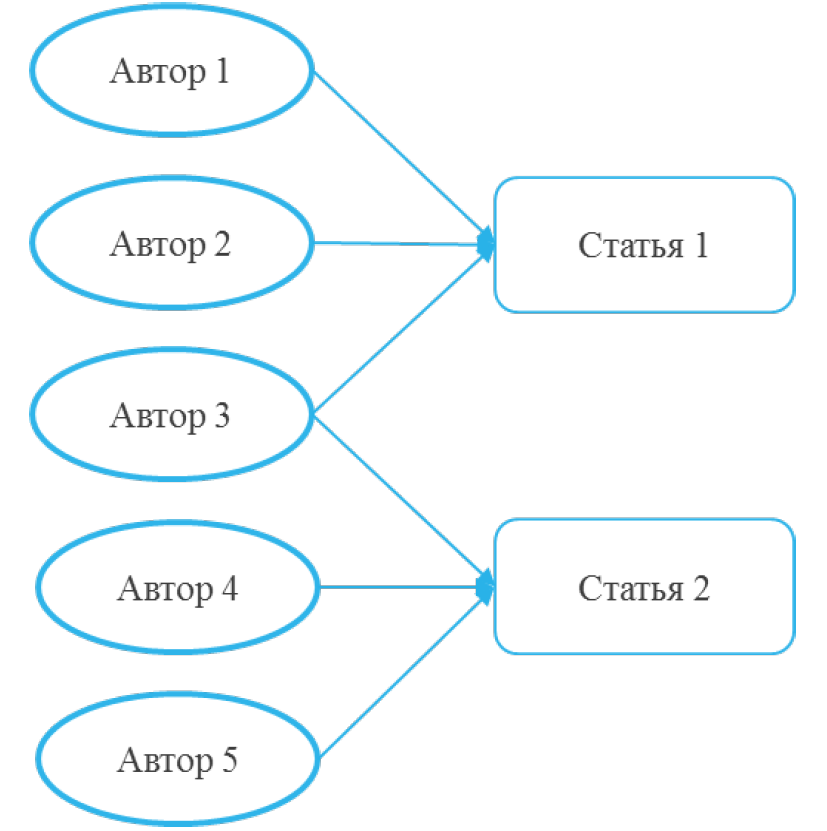
\includegraphics[width=0.8\textwidth]{bi_fig1}
  \label{fig:bi1}
  \caption{Двудольный граф соавторств.}
\end{figure}  
 
Преимущества такого подхода состоят в том, что в графе соавторств становится возможным сохранить для дальнейшего анализа библиографическую информацию о статье: 

\begin{enumerate}
\tightlist
\item Название статьи 
\item Год издания 
\item Издатель 
\item Ключевые слова 
\end{enumerate}

Отметим, что традиционное представление графа соавторств в виде неориентированного графа является проекцией двудольного графа на множество вершин авторов. 
Поясним это более подробно. 
Ориентированный граф $G = (V,E)$  называется двудольным, если множество его вершин можно разбить на две части $ A \cup P = V$, так, что 
\begin{itemize}
	\item ни одна вершина в $A$ не соединена с вершинами в $P$
	\item ни одна вершина в $P$ не соединена с вершинами в $A$. 	
\end{itemize}

В рассматриваемом случае $A$ - это множество авторов, $P$ - это множество статей. $A$ и $P$ - являются долями графа $G$.
Отметим, что граф $G$ может быть как полным так и неполным в зависимости от того имеют ли авторы соединения со всеми статьями. 
Приведенный на Рисунке \ref{bi_fig1} двудольный граф является неполным. 
Обозначим  $G_A$ проекцию графа  $G$ на множество вершин $A$.
Граф $G_A$ является традиционным представлением графа соавторств и отображен на рисунке \ref{fig:bi2}. 

\begin{figure}[H]
  \centering
    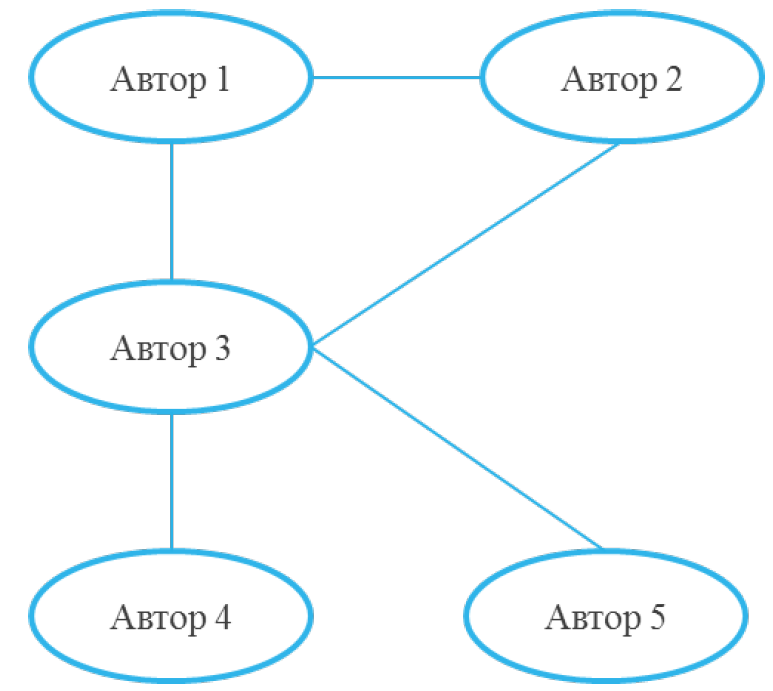
\includegraphics[width=0.8\textwidth]{bi_fig2}
  \label{fig:bi2}
  \caption{Неориентированный граф соавторств.}
\end{figure}  

Из рисунка \ref{fig:bi2} видно, что при построении проекции атрибутами ребер графа $G_A$ могут стать только интегральные характеристики соавторства, например, количество соавторств двух авторов.

\subsection{Моделирование графов соавторства}
Для моделирования графов соавторства как социальной сети широко применяется следующие стохастические подходы: 
\begin{enumerate}
\item Случайные графы.
\item Модель ``Маленький мир'' (small-world).
\item Модели, основанные на концепции преимущественного присоединения (preferential attachment).
\end{enumerate}

Одним из существенных ограничений стохастических моделей является фиксированное количество рассматриваемых вершин, или их постоянный рост. 
На практике в организации изменяется количество потенциальных соавторов.
Так же важно понимать, что стохастические модели ставят целью моделировать граф с определенными параметрами. 
Такими как, кластеризация, плотность и др.

С другой стороны, формирование малых групп, к которым относится и группа соавторов научной статьи, моделируется на основании принципа дополнительных компетенций, относящегося к классу детерминированных методов создания графов соавторства. 

Для предсказания новых вершин графа соавторства применяется комбинированный подход на основе машинного обучения с предварительным отбором признаков авторов, статистических показателей активности за несколько последних временных промежутков, а также структурные индексы влияния и локальные метрики в сети соавторства. 
Полученные в данной работе результаты позволили сделать вывод о применимости методов предсказания связей для анализа коллаборативных шаблонов поведения в крупной организации с динамической структурой коллектива, а также меняющимися внешними и внутренними факторами, влияющими на индивидуальную и коллективную публикационную активность.

Основой для прогнозирования изменений графа соавторств для научно-технического центра являются следующие компоненты: 
\begin{itemize}
\item Текущая структура графа соавторств.
\item Внешние по отношению к научно-техническому центру воздействия.
\item Внутренние изменения научно-технического центра. 
\end{itemize}

Рассмотрим каждую из компонент подробнее. Текущая структура графа соавторств представляет набор метрик, описывающих данный граф соавторств.
К таким метрикам принято относить следующие: 
\begin{itemize}
\item Для ребер
\begin{itemize}
\item Common Neighbours (CN)
\item Salton Index (SI)
\item Jaccard Index (JI)
\item Hub Promoted Index (HPI)
\item Hub Depressed Index (HDI)
\item Leicht-Holme-Newman Index (LHN1)
\item Preferential Attachment Index (PA)
\item Adamic-Adar Index (AA)
\item Resource Allocation Index (RA)
\end{itemize}
\item Для вершин 
\begin{itemize}
\item Degree centrality
\item Betweenness centrality
\item Closeness centrality
\item Harmonic centrality
\item Clustering
\end{itemize}
\end{itemize}

Каждая из этих метрик представляет характерный набор признаков (features) графа соавторств, влияющих на прогноз его изменений. 
Внешние по отношению к научно-техническому центру воздействия заключаются в публикационной политике редакций, публикующих научные статьи. 
В простейшем случае отсутствие возможности опубликовать статью из-за ограничений по объему выпуска журнала приводит несостоявшемуся соавторству. 
Основные зависимости публикационной активности научно-технического центра от редакций рассмотрены в работе \cite{krasnov2017model}.
Внутренние изменения научно-технического центра вызваны изменениями в составе персонала. 
В организацию приходят новые сотрудники, некоторые сотрудники увольняются.
В процессе наставничества и обучения сотрудники приобретают новые компетенции. 
В результате проведения НИР рождаются новые исследования и научные заделы. 
Часто, изменения внутренних требований к качеству публикаций также могут стать причиной структурных изменений, подтверждая принцип “publish or perish”, и влияя как на структуру коллектива, так и на параметры активности отдельных сотрудников и исследовательских коллективов.
Рассмотрим подробнее в чем состоит прогноз развития графа соавторств для научно-технического центра. 
Под развитием будем понимать возникновение новых вершин и ребер. 
Граф соавторств может рассматриваться как накопленным итогом за период, так и инкрементальными изменениями по годам. 
Далее будем рассматривать факт авторства, как признак вершины графа соавторств.
Другими словами, сотрудник, представляемый вершиной графа соавторства, может как написать, так и не написать статью в следующем временном периоде. 
Процесс прогнозирования в данном случае будет решать задачу бинарной классификации. 
Для каждого сотрудника будет определяться вероятность создания статьи по определенной тематике. 
Статья является коллективным усилием работы соавторов, обладающих определенным набором компетенций, нашедших свое применение в цели исследования.
В этом состоит основная идея принципа дополнительности компетенций. 
Авторы с одинаковыми компетенциями не имеют рационального обоснования для объединения с целью проведения научного исследования. 
Будем считать, компетенции атрибутами вершин графа.  
Для выявления компетенций необходимых для написания статьи будем использовать ключевые слова, а при их отсутствии – метод тематического моделирования текста работы.

\section{Современные процессы организации труда на основе гибких методик}

Гибкие (Agile) методики разработки программного обеспечения широко применяются в различных индустриях. 
Написание программного кода по своей сути является процессом создания логически структурированного текста так же, как и написание научной статьи. 
Коллективная работа над написанием научных статей требует разделения обязанностей для повышения продуктивности так же, как и написание программного кода требует выделения специалистов для тестирования и документирования.

Использование ролевой модели гибких методик представляется перспективным кросс-индустриальным опытом для применения, но нуждается в теоретической проверке. Одним из вариантов проверки гипотез, показавшим себя в условиях, когда постановка реального эксперимента представляется высоко затратной, является метод имитационного моделирования. 
Автор видит дополнительные преимущества от институциализации процесса написания научных статей и применения проверенных индустриальных показателей эффективности для его оценки.

Провозглашение основных принципов гибких методик в виде манифеста \cite{fowler2001agile} обозначило насущную необходимость перехода к более эффективным методам разработки программного обеспечения. 
Решительность этого шага многократно себя оправдала на практике и в последствии нашла теоретические обоснования {bonner2016empirical}. 
Суть гибких методик может быть изложена по-разному, но для данного исследования нами выбрана следующая формулировка:

\begin{enumerate}
\tightlist
\item Приоритет командных взаимодействий
\item Приоритет работающего программного кода
\item Приоритет реакций над планом
\end{enumerate}

Современные методики написания научных статей остаются на позициях последовательного, ``водопадного'' подхода.
Такой подход был уместен во времена Ньютона, когда один уникальный ум работал над трудом всей своей жизни.
В условиях современной скорости обмена научной информацией одиночки остаются не у дел.
Им на смену приходят научные коллективы.
Интуитивно понятно, что от согласованной работы научного коллектива соавторов зависит их продуктивность: оптимальное соотношения качества и скорости публикации результатов научных исследований в виде научных статей, доступных наиболее широкому кругу заинтересованных лиц. 
В гибких методиках разработки программного обеспечения образование команды основано на принципах самоорганизации \cite{hoda2016multi,moe2008understanding}.
Самоорганизующиеся команды  в работе \cite{moe2009overcoming} разделены на три типа:

\begin{enumerate}
\tightlist
\item  ``Команда пилотов самолёта'': Управление воздушным судном.
\item  ``Компьютерные команды'': Создание новых программных продуктов.
\item  ``Команда КВН'': Решение сложных проблем.
\end{enumerate}

Для целей дальнейшего исследования нас больше будут интересовать тип ``Компьютерные команды''.

\subsection{Размеры команд}

Размеры команд играют важную роль. 
В гибких методиках разработки программного обеспечения рассматриваются малые (5-7), большие (10-50) и сверхбольшие команды (100-200) \cite{alnuaimi2010team}.

Важно отметить, что приведенные оценки сходятся с полученными в работе \cite{kradoya2016structure} для команд соавторов: современные творческие команды соавторов в среднем состоят из 3 участников. 
В дальнейшем изложении будем подразумевать, что число участников команды состоит в среднем из 3 соавторов.

\subsection{Образование команд}

Гибкие методики \cite{fowler2001agile} подразумевают под самоорганизацией только возможность работы команды с ограниченным управлением из вне. 
На взгляд автора данного исследования, целесообразно рассмотреть, как образуются команды в деталях.

Для рассмотрения механизма необходимо понимать, что команда образуется с определённой целью. 
Рассматривая образование команд авторы исследования \cite{guimera2005team} предлагают эмпирический вероятностный алгоритм присоединения нового участника к уже сформированной группе (Рис.\ref{ex:fig2_1}):

\begin{figure}[H]
  \centering
    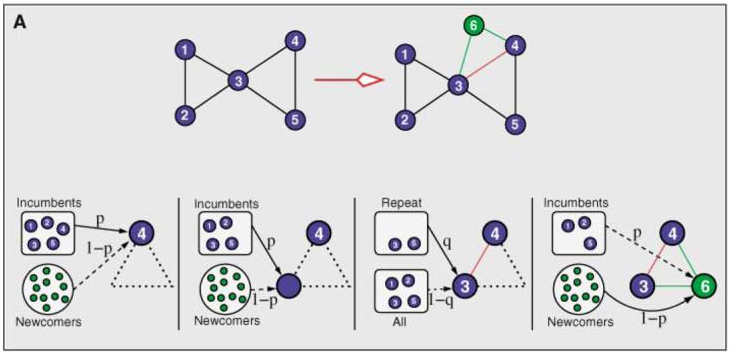
\includegraphics[width=0.8\textwidth]{guimera2}
  \label{ex:fig2_1}
  \caption{Алгоритм образования команд на основе вероятностей (p - для новых участников, q - для участников группы) \cite{guimera2005team}}
\end{figure}
 
Таким образом, авторы работы \cite{guimera2005team} оценивают влияние внутренней структуры команды на её расширение.

В работе \cite{moe2009overcoming} отмечено, что основным фактором для самоорганизации команд являются индивидуальные компетенции.
При этом компетенции каждого участника оцениваются с точки зрения полезности для достижения цели. 
В исследованиях \cite{berger1972status,berger1980status} утверждается, что такая оценка приводит к появлению системы статусов участников команды, которая выражается в иерархичности коммуникаций. 
Для настоящего исследования нам достаточно того, что:
\begin{enumerate}
\tightlist
\item  Цель является образующим базисом для команды;
\item  Цель декларирует потребности в компетенциях участников команды;
\item  Участники производят оценку компетенций друг друга для достижения цели.
\end{enumerate}

Базовый алгоритм образования команды для двух участников может быть представлен в виде следующей временной последовательности (\ref{ex:fig2}):

\begin{figure}[H]
  \centering
    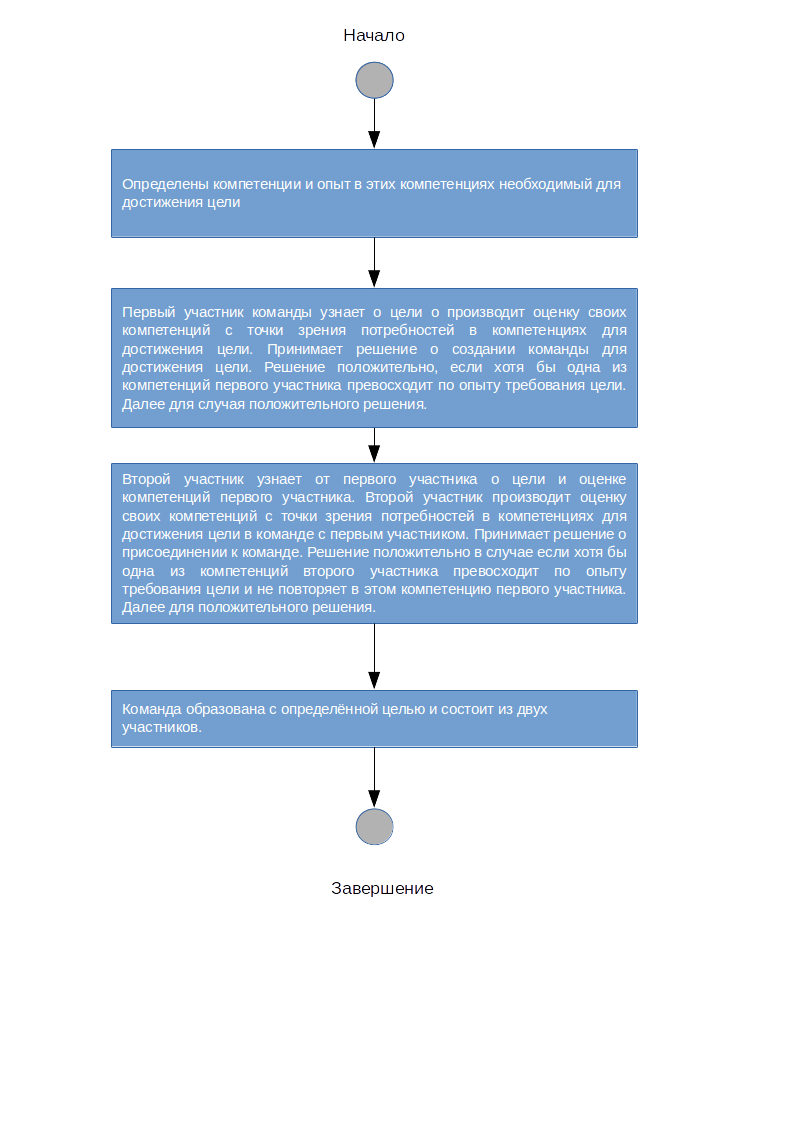
\includegraphics[width=0.8\textwidth]{ex_fig2}
  \label{ex:fig2}
  \caption{Базовый алгоритм образования команды.}
\end{figure}


Приведенная на Рис. \ref{ex:fig2} последовательность описывает основное образующее команду действие - \textit{парное объединение}.
Можно сказать, что после присоединения участников у команды появляется собственный профиль компетенций для достижения заданной цели. 
Компетенции команды получаются в результате суперпозиции компетенций участников. 
Некоторые из компетенций необходимых для достижения цели ``закрыты опытом'' участников, а некоторые нет.
Следующий за первым участник присоединяется уже с учётом профиля компетенций команды. 
Для удобства дальнейшего изложения сформулируем следующие утверждения:

\begin{state}[У\ref{state:1}] \label{state:1}
Сотрудники объединяются в команду для достижения цели.
\end{state}

\begin{state}[У\ref{state:2}] \label{state:2}
Компетенции команды являются функцией от компетенций участников.
\end{state}

\begin{state}[У\ref{state:3}] \label{state:3} 
Объединение первого участника с командой
для достижения цели происходит по таким же принципам, что и объединение
команды из n участником с n+1 участником. 
\end{state}

\subsection{Парное объединение}

Рассмотрим подробнее \emph{парное объединение}. 
Организационная среда задает размерность $N_{comp}$ пространства компетенций. 
Каждый участник организационной среды $a$ обладает вектором компетенций $c_i$ таких, что $i \in N_{comp}$. 
Каждая компетенция участника $c_i$ характеризуется опытом $e_i$ . 
Опыт участника -- это натуральное число, $e_i \in \mathbb{N}$. 
В результате можно сказать, что  участник обладает вектором опыта в пространстве компетенций. 
Отметим, что пространство компетенций организационной среды обладает существенно большей размерностью, чем вектор компетенций участника.
Изначально команда $t_0$ не содержит участников и не обладает собственными компетенциями (Рис. \ref{ex:fig3}).

\begin{figure}[H]
  \centering
    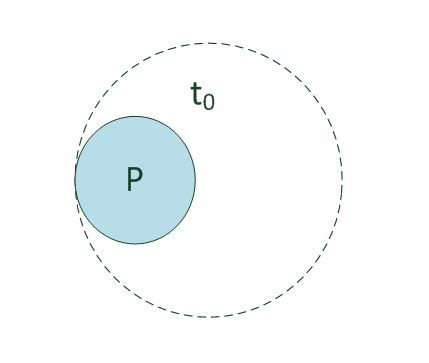
\includegraphics[width=0.5\textwidth]{scrum_fig3}
  \label{ex:fig3}
  \caption{Схема команды без участников.}
\end{figure}

Пусть $P$ обозначает цель для объединения команды, $c_j$ -- вектор компетенций, а $e_j$ -- опыт по каждой компетенции необходимый для достижения $P$. 
В результате успешного объединения для достижения цели будет образована команда $t_1$(Рис. \ref{ex:fig4}).

\begin{figure}[H]
  \centering
    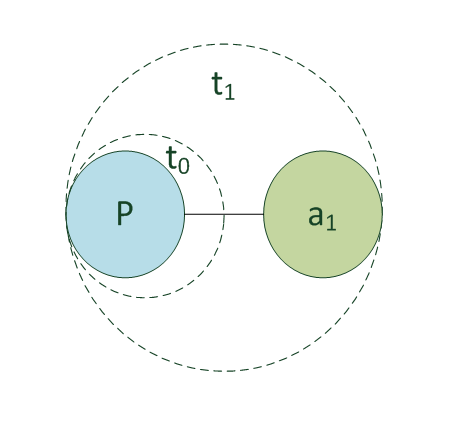
\includegraphics[width=0.5\textwidth]{scrum_fig4}
  \label{ex:fig4}
  \caption{Схема команды из одного участника.}
\end{figure} 

Команда $t_1$ обладает новым вектором компетенций. 
Так как в $t_1$ только один участник $a_1$, то вектор компетенций $t_1$ будет совпадать с вектором компетенций $a_1$. 
При присоединении к  $t_1$ участника $a_2$ будет образована команда $t_2$ (Рис. \ref{ex:fig5}).

\begin{figure}[H]
  \centering
    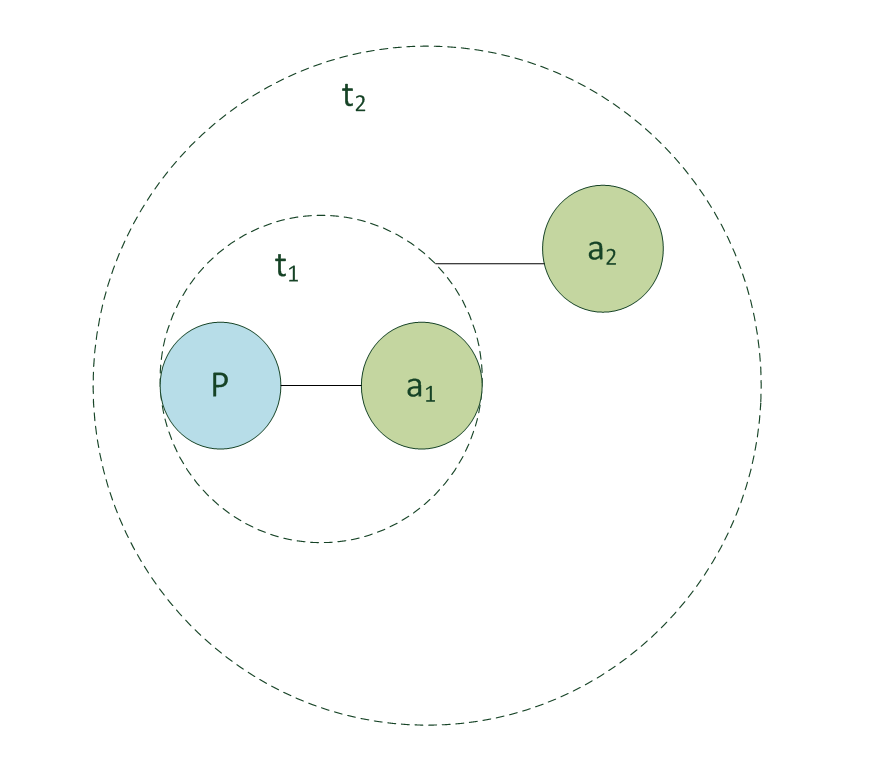
\includegraphics[width=0.8\textwidth]{scrum_fig5}
  \label{ex:fig5}
  \caption{Схема команды из двух участников.}
\end{figure} 


Так как участник присоединяется ко всем элементам команды , то можно привести схему (Рис. \ref{ex:fig5}) к виду графа команды (Рис. \ref{ex:fig6}).

\begin{figure}[H]
  \centering
    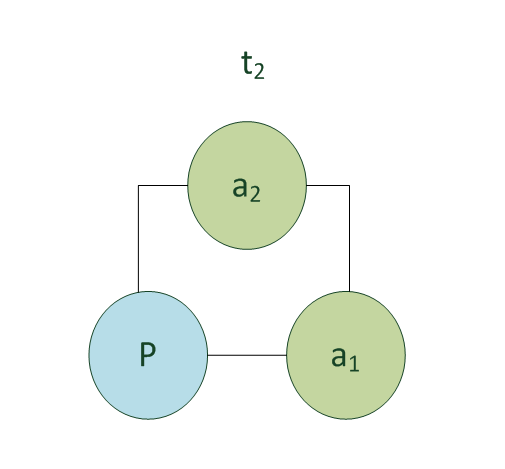
\includegraphics[width=0.8\textwidth]{scrum_fig6}
  \label{ex:fig6}
  \caption{Граф команды из двух участников с избыточными связями.}
\end{figure}  

Цель является $P$ атрибутом ребра, связывающего $a_1$ и $a_2$, поэтому можем преобразовать граф команды с двумя участниками к виду (Рис. \ref{ex:fig7}).

\begin{figure}[H]
  \centering
    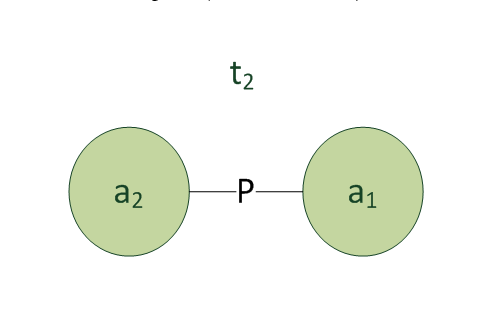
\includegraphics[width=0.8\textwidth]{scrum_fig7}
  \label{ex:fig7}
  \caption{Граф команды из двух участников.}
\end{figure}  

Для случая написания научных статей граф команды $t_2$, изображенный на Рис.\ref{ex:fig7} обозначают $g(t_2)$ и называют графом соавторства, где под $P$ подразумевают научную статью.
Информация о истории создания команды в такой нотации не приводится. 
На Рис.\ref{ex:fig8} приведен пример фрагмента графа соавторства.
Вершинами графа являются исследователями, а ребрами -- совместная научная публикация. 
Граф соавторства является ненаправленной сетью.
\begin{figure}[H]
  \centering
    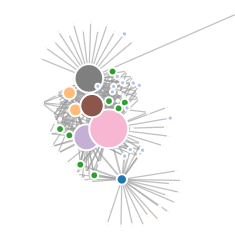
\includegraphics[width=0.5\textwidth]{scrum-img8}
  \label{ex:fig8}
  \caption{Фрагмента графа соавторства для нескольких команд.}
\end{figure}  

Отметим, что для наглядности на Рис.\ref{ex:fig8} размер вершин отражает количество научных статей, написанных участником.

\subsubsection{Командный код}

Введем понятия \emph{полного командного кода} \emph{(ПКК)} и \emph{остаточного командного кода (ОКК)}.
Эти понятия играют ключевую роль в образовании команды. 
Составляющими командного кода являются компетенции. По своему типу \emph{полный} и \emph{остаточный} \emph{командный код} -- это вектора в пространстве $N_{comp}$ .

Рассмотрим, как участником производится оценка своих компетенций с точки зрения потребностей в компетенциях для достижения цели.

Характеристики цели $P$ являются основанием для образования команды. 
То есть, первый участник команды $a$ и цель $P$ должны быть объединены на основании представления о компетенциях. 
Другими словами, необходимыми условиями для достижения цели должно быть обладание $a$ определенным набором компетенций и опыта. 
С точки зрения множеств компетенции сотрудника $a$ и цели $P$ должны находиться в одном пространстве и иметь пересечения. 
Наличие пересечений будет приводить к объединению в команду.

Введем функцию оценки в виде $\Phi(P,t,a), \Phi \in [0,1] $. 
Результатом $\Phi$ будет вероятность возможности объединения участника $a$  в команду $t$ для достижений цели $P$. 
Тогда функция $\Phi$ для $n$-ого участника может быть записана в виде $\Phi_n(P,t_{n},a_n)$.

По мере присоединения участника вектор компетенций команды будет изменяться.
В него будут входить компетенции новых участников, а опыт по одинаковым компетенциям будет складываться.

\begin{equation} 
\label{eq:scrum1}
ut_{n-1} = \prod_{a_j}^{a_{n-1}}\sum_i^{N_{comp}}\bigg\{c_j * \, e_i \bigg\}
\end{equation}

Величину $ut_{n-1}$ будем называть \emph{полным командным кодом (ПКК)}. 
\emph{ПКК} характеризует потенциал команды для достижения целей.

В соответствии с вышеописанным алгоритмом (Рис. \ref{ex:fig2}) функцию $\Phi$ можно представить в виде:

\begin{equation} 
\label{eq:scrum2}
\Phi  = P \cdot \prod_{a_j}^{a_{n-1}}\sum_i^{N_{comp}} \bigg\{c_j *\, e_i \bigg\} \cdot a_n
\end{equation}

Важную смысловую часть в выражении (\ref{eq:scrum2}) несет компонент $rt^P_n$, который автор называет \emph{остаточным командным кодом}  -- \emph{ОКК}.

\begin{equation} 
\label{eq:scrum3}
rt_n^P  = P \cdot \prod_{a_j}^{a_{n-1}}\sum_i^{N_{comp}} \bigg\{c_j *\, e_i \bigg\}
\end{equation}

\emph{ОКК} $rt_n^P$ характеризует незакрытые $t_n$ командой компетенции цели $P$. 
Нулевой вектор в качестве \emph{ОКК} характеризует полную укомплектованность компетенциями команды для достижения цели.

С учетом \emph{ОКК} можно преобразовать выражение (\ref{eq:scrum2}) следующим образом:

\begin{equation} 
\label{eq:scrum4}
\Phi  =  rt_n^P \cdot a_n 
\end{equation}

Выражение (\ref{eq:scrum4}) имеет интуитивно понятный смысл: 
\emph{для оценки возможности присоединения к команде новый участник должен выяснить обладает ли он необходимым опытом в требуемых для выполнения цели компетенциях с учетом того, что существующая команда уже закрыла часть из необходимых компетенций своим опытом}. 
В работах \cite{hamilton2003team,prat2002should} такой принцип образования команд называют комплементарным.

\subsubsection{Гомогенность команд}

Мы рассмотрели образование команд на основе дополнительности (комплементарности) компетенций. 
Второй движущей силой для образования команд является гомогенность.

Гомогенность групп в социальных сетях, или склонность людей со схожими характеристиками формировать связи между собой, также называемая гомофилией, является важным фактором формирования и эволюции социальных сетей \cite{mcpherson2001birds}. 
Во многих работах отмечается динамическая структура гомофилии \cite{snijders2010introduction,steglich20108}, в ходе которой параллельно происходят два процесса.
С одной стороны -- схожие между собой индивиды формируют социальные связи (социальная селекция). 
С другой -- уже связанные друг с другом люди перенимают поведение друг друга (социальное влияние).
Совокупность этих факторов результирует в гомогенную социальную систему, в которой между индивидами со схожим поведением и характеристиками есть связь, при этом характер связи может быть, как формальным, так и неформальным.

Несмотря на то, что связи между индивидами со схожими характеристиками более вероятны, чем связи между непохожими, уровень схожести также важен.
В работе \cite{block2014multidimensional} было показано, что социальная схожесть более, чем по одному показателю, приводит к тому, что люди с меньшей вероятностью будут формировать между собой взаимоотношения. 
Автор объясняет данный эффект тем, что слишком схожие по многим характеристикам люди, как правило, не могут привести что-то новое и конструктивное во взаимные отношения или же в команду.
Для продуктивного сотрудничества необходима не только схожесть интересов, но также и различный профессиональный и жизненный опыт, позволяющий предложить многомерные подходы к ее решению.

Основным объединяющим фактором в команде являются компетенции участников, влияющие на достижения цели.
Основываясь на понятии \emph{ОКК}, введенного ранее, можно рассмотреть остаточные компетенции участника, то есть компетенции, не востребованные для объединения команду для достижения цели. 
Влияние этой части компетенций на команду может как усиливать ее, так и ослаблять во время работы.

\subsubsection{Работа команд}

Начало работ по достижению цели определяется участниками команды и не зависит от процесса образования команды. 
Показатели производительности могут быть только у работающей команды. 
Например, важное для научной сферы деятельности понятие \emph{научный} \emph{задел} означает ни что иное как работы, выполненные командой имеющей не пустой \emph{остаточный} \emph{командный код.}

Формирование основной системы внутреннего взаимодействия внутри команды согласно исследованию \cite{harper1985power} происходит при знакомстве участников.
Таким образом, для данного исследования будем пренебрегать временем установления устойчивой работы каналов коммуникаций.

В гибких методиках разработки программного обеспечения наибольшее внимание уделяется именно коммуникациям внутри команды \cite{boehm2003people} и с внешними агентами \cite{paasivaara2012experiences}, которые по сути тоже являются командой, но в более широком смысле.

Сформулируем следующее утверждение:

\begin{state}[У\ref{state:4}] \label{state:4}
Характеристики работы каналов коммуникаций соответствуют характеру работы команды.
\end{state}

Таким образом, измеряя работу коммуникационных каналов можно сделать заключения о характере работы команды.
Отметим, важное следствие: такой тип измерения производительности команды не создаёт дополнительной нагрузки на сотрудников в отличии от методик оценки основанных опросах.

Вопрос измерения вклада отдельных участников или результата команды рассмотрен в ряде работ \cite{tannenbaum2013team,hill1982group} и все исследователи склоняются к тому, что измерять нужно и командную производительность (Team Performance), и индивидуальная продуктивность (Individual Performance).
В исследовании \cite{tims2013job} приведена следующая схема измерений (Рис. \ref{ex:fig9}).

\begin{figure}[H]
  \centering
    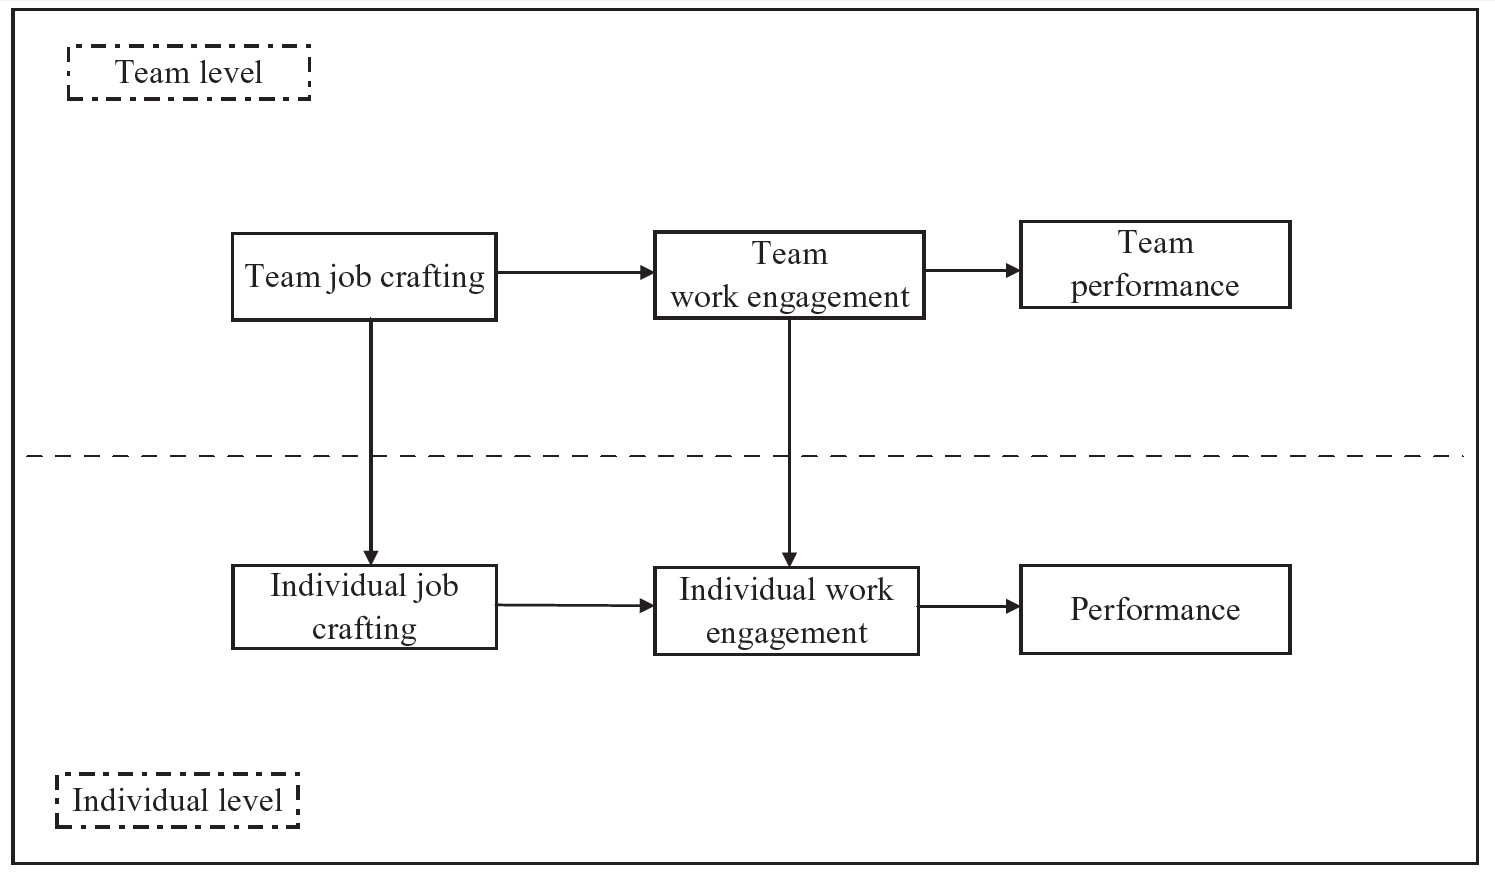
\includegraphics[width=0.8\textwidth]{scrum-img9}
  \label{ex:fig9}
  \caption{Уровни измерения производительности команды и участника \cite{tims2013job}.}
\end{figure}  

Например, измерение Individual Performance с помощью опросов исследуется в работе \cite{cropley2012measuring} путём введения Creative Solution Diagnosis Scale (CSDS) -- шкалы креативности. 
Измерить Individual Performance сотрудника по такой шкале авторы \cite{cropley2012measuring} предлагают с помощью Consensual Assessment Technique (CAT), которая требует дополнительных усилий от сотрудников.
Сильные и слабые стороны метода опросов для измерения Individual Performance изложены в фундаментальной работе \cite{jackson1965person}.

Вопрос метода измерения Individual Performance находит интересную постановку в современной концепции ``sensible organization'' \cite{olguin2008sensible}.
Авторы исследования \cite{olguin2008sensible} помимо измерения традиционных цифровых коммуникационных каналов надевают на сотрудников браслеты, отслеживающие перемещения и другие параметры организма.

Вопросы зависимости производительности команд от структуры команд рассмотрены в исследовании \cite{kradoya2016structure}.

\subsubsection{Методика Scrum}
Одной из распространённых гибких методик командной работы является методика Scrum \cite{sutherland2013scrum}. 
Scrum предназначен для получения наилучших из возможных результатов для командной разработки сложных интеллектуальных продуктов.
В классическом Scrum существует 3 базовых роли:

\begin{itemize}
\tightlist
\item  Product owner -- отвечает за соответствия целям
\item  Scrum master -- отвечает за эффективное взаимодействие в команде
\item  Команда разработки (Development team)
\end{itemize}

Рекомендуемый размер Scrum команды --- 5-7 человек соответствует принятым в данном исследовании ограничениям.
Согласно идеологам Scrum \cite{sutherland2013scrum}, команды большего размера требуют значительных ресурсов на коммуникации, в то время как команды меньшего размера уменьшают размер работы, который команда может выполнить в единицу времени.

Основой Scrum является Sprint, в течении которого выполняется работа над продуктом. 
Sprint имеет одинаковую продолжительность на протяжении всего процессы создания продукта, рекомендуется одна неделя. 
Задача Sprint состоит в том, чтобы материализовать продукт в текущем виде. 
Продуктом в данном исследовании является научная статья.

Методика Scrum декларирует необходимость в определенных видах деятельности, не связанных с исследованиями и написанием текста, которые приводят к лучшей результативности. 
Кроме этого Scrum задает определенный ритм для этих дополнительных деятельностей.

Введем показатели, на которые влияет применение Scrum к процессу написания научных статей:

\begin{enumerate}
\tightlist
  \item   Ускорения обмена сообщениями в каналах коммуникаций;
  \item   Потеря работ из-за дублирования при отсутствии своевременных коммуникаций о прогрессе проведения исследований;
  \item   Потеря работ из-за несоответствия написанной статьи правилам  публикации.
\end{enumerate}

С точки зрения формализма графа соавторства применение Scrum приведет к выделению вершин графа, обеспечивающих функции \emph{Product owner (PO)} и \emph{Scrum master (SM)} (Рис.\ref{ex:fig10})

\begin{figure}[H]
  \centering
    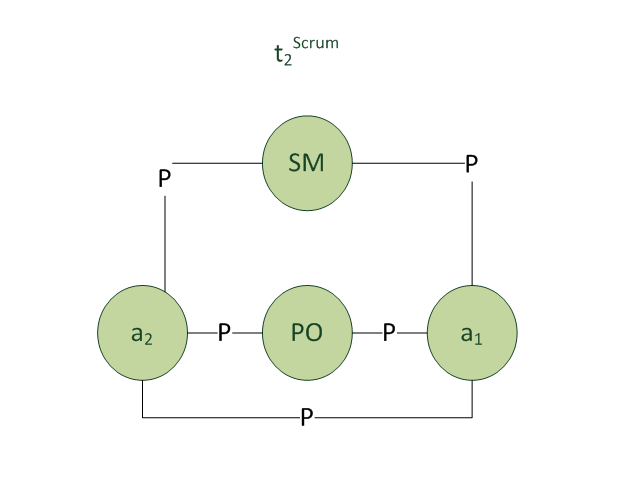
\includegraphics[width=0.8\textwidth]{scrum_fig10}
  \caption{Соавторство с ролями Scrum.}
  \label{ex:fig10}
\end{figure}  

С графом $g(t_2^{Scrum}$), отображенным на Рис.\ref{ex:fig10} можно произвести преобразование аналогичное сделанному выше с графом $g(t_2)$. 
Как мы видим, Scrum роли PO и SM соединяют вершины $a_1$и $a_2$. 
Из чего следует, что PO и SM являются характеристиками ребер графа, соединяющего $a_1$ и $a_2$. 
Преобразованный граф соавторства с применением Scrum ролей отображен на Рис. \ref{ex:fig11}.

\begin{figure}[H]
  \centering
    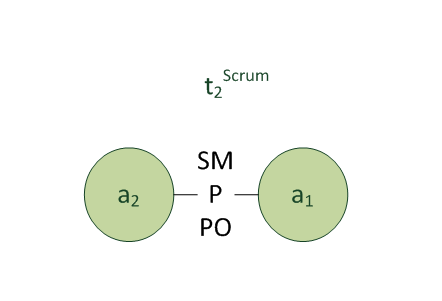
\includegraphics[width=0.8\textwidth]{scrum_fig11}
  \caption{ Граф соавторства с атрибутами Scrum.}
  \label{ex:fig11}
\end{figure}  

Роли Scrum согласно \cite{fowler2001agile} не должны вмешиваться в содержательную часть работы команды, а лишь ускорять информационный обмен и устранять информационные барьеры.
Сформулируем это в виде гипотезы, формальное доказательство которой отложим для дальнейших исследований:

\begin{hyp}[Г\ref{hyp:ex1}] \label{hyp:ex1}
Введение ролей Scrum в процесс соавторства не изменяет вид графа соавторства.
\end{hyp}

Теперь рассмотрим показатели производительности работы команд.

\subsubsection{Показатели производительности команд}

В современной работе \cite{pereme2016toward} рассмотрены вопросы разработки показателей, измеряющих скорость перехода продукта из фазы исследований (research) в фазу разработки (development). 
Авторами \cite{pereme2016toward} предложена интегральная модель для таких показателей. 
Объектом измерения авторы считают знания, а показатели основывают на процессе Knowledge Management. 
Никаких конкретных KPI авторы не предлагают, но описывают пространственные оси своей модели -- процессы, инструменты и люди.

Связь между способностью команды собраться и ее продуктивностью исследовали в работе \cite{edwards2006relationships}. 
Стоит отметить, что в работе \cite{edwards2006relationships} образование команды подразумевает формирование, а не самоорганизацию.

Состав команды во времени не постоянен и говорить от том, что образование команды в тот или иной момент времени завершено не корректно.
Участники могут покидать команду и участвовать в нескольких командах одновременно. 
Важная веха в работе команды определяется нулевым \emph{ОКК}, когда все компетенции необходимые для достижения цели представлены участниками команды. 
Сформулируем это в виде утверждения:

\begin{defi}[О\ref{defi:ex1}] \label{defi:ex1}
Команда считается укомплектованной, тогда и только тогда, когда ее ОКК равен нулевому вектору в пространстве $N_{comp}$.
Минимальное время, в котором ОКК стал равен нулевому вектору называется Временем комплектации ($T_c$).
\end{defi}

Отметим, что $T_c$ может быть больше времени, отведенного издательством или программным комитетом научной конференции на подготовку. 
Таким образом, статья не будет обладать требуемыми качествами в срок и не будет принята к публикации.

Показатели, наиболее точно отражающие динамику выполнения работы, будут основываться на изменении в динамике всех параметров команды. 
Введем функцию применения командой опыта в определенных целью компетенциях: $E(P,t)$.
Факторами, негативно влияющими на $E$ будут сложность коммуникаций внутри команды $\Xi(g)$ и необходимость заниматься деятельностью, не направленной на создания научных статей $\Gamma(t)$ .

И $\Xi(g)$, и $\Gamma(t)$ будут увеличивать время, требуемое на написание научной статьи.
Таким образом, команда может не достигнуть цели в определенные сроки.

Сформулируем две рассмотренные причины не достижения командой цели:

\begin{defi}[О\ref{defi:ex2}] \label{defi:ex2}
Несостоявшейся научной статьей (ННС) будем считать статью, не уложившуюся во временные рамки публикационного процесса с требуемым качеством. 
\end{defi}

Отношение количества несостоявшихся статей ($Frac_{notpub}$) к количеству опубликованных статей является показателем производительности процесса написания научных статей.

Другим более очевидным показателем производительности является время, затраченное на публикацию научной статьи ($T_{pub}$).

\section{Анализ текста}
\label{sec:topicmodel}
\subsection{Анализ текста на основании тематик}
%% Topics
В последние годы бурно развиваются методики тематического моделирования. Недавние исследования привели к развитию нескольких основных направлений: вероятностного [1], на основе SVD [2] и генеративного [4].
Тематическое моделирование определяет каждую тему как распределение некоторого количества слов с определенными вероятностями. Большинство современных тематических моделей строятся на основе распределения Дирихле (LDA, Latent Dirichlet Allocation) [3].
Трудно представить, что настолько универсальное распределение как LDA будет одинаково хорошо работать для любых текстов. 
Необходимы тонкие настройки алгоритма на конкретный проблемный домен. 
Поэтому автор сосредоточился на основном мировом источнике для научно-практических статей нефтегазовой отрасли – библиотеке OnePetro. 
Важно отметить, что OnePetro охватывает широкий спектр инженерных дисциплин и содержит тексты на английском посвященные именно практическим аспектам применения новых технологий в нефтегазовой отрасли. 
Авторами этих статей являются сотрудники нефтяных компаний со всего мира.
%% 

Формальная постановка задачи тематического моделирования следующая. 
Пусть зафиксирован словарь терминов $W$, из элементов которого складываются документы, и дана коллекция $D$ документов $d \in D$. 
Для каждого документа $d$ известна его длина $n_d$ и количество $n_dw$ использований каждого термина $w$.
Пусть $\Phi=(\phi_{wt})$ - матрица распределений терминов ($w$) в темах ($t$), а  $\Theta=(\theta_{td})$  - матрица распределений тем ($t$) в документах ($d$). 
Тогда задача тематического моделирования состоит в том, чтобы найти такие матрицы  $\Phi$ и $\Theta$, чтобы выполнялось равенство (\ref{eq:op3_1}).

\begin{equation} 
\label{eq:op3_1}
p ( w \vert d ) = \sum_{t \in T} \phi_{wt} \theta_{td},
\end{equation}
где $ \phi_{wt} $ - вероятности терминов $w$ в каждой теме $t$, $\theta_{td}$ – вероятности тем $t$ в каждом документе $d$, а $ p ( w \vert d ) $ – вероятность появления термина $w$ в документе $d$.

Уравнение (\ref{eq:op3_1}) можно представить в матричном виде $ \Phi \cdot \Theta $. 
При этом легко показать, что данная задача имеет много решений (\ref{eq:op3_2}). 
\begin{equation} 
\label{eq:op3_2}
\Phi \cdot \Theta  = \Phi \cdot \Lambda \cdot \Lambda^{-1} \cdot \Theta = \hat{\Phi} \cdot \hat{\Theta},
\end{equation}
где $\hat{\Phi} = \Phi \cdot \Lambda $, а  $\hat{\Theta} = \Lambda^{-1} \cdot \Theta$.

Из уравнения (\ref{eq:op3_2})  следует, что матрицы $\hat{\Phi}$ и $\hat{\Theta}$ так же будут являться решениями уравнения (\ref{eq:op3_1}).
Но не все матрицы $\Phi$ и $\Theta$ будут содержать хорошо интерпретируемые тематики. 
Таким образом, в задачу (\ref{eq:op3_1}) необходимо ввести условия способствующие получению адекватных и интересных тематик. 
Образно можно сказать, что необходимо оцифровать специфику предметной области текста для встраивания в алгоритм поиска оптимальных матриц $\Phi$ и $\Theta$. 
Отметим, что при использовании LDA для создания тематической модели такой настройки на предметную область не производится.
Для решения подзадачи настройки тематической модели на предметную область автором использован механизм регуляризаторов. 

Пусть $p \left( t \right) $ — распределение тем в коллекции документов:
\begin{equation} 
\label{eq:op3_3}
p \left( t \right) = \sum_d p \left( d \right)  \theta_{td}
\end{equation}

Тогда полезным представляется регуляризатор на основе дивергенции Кульбака-Лейбнера: 
\begin{equation} 
\label{eq:op3_4}
\mathcal{KL}(\Theta)= -\tau \sum_{t \in T} \ln \bigg( \sum_{d \in D} p \left( d \right) \theta_{td} \bigg) \rightarrow max
\end{equation}

Где $\tau$ – параметр регуляризации, который нужно подобрать в зависимости от предметной области коллекции документов. 
Требование максимизации $\mathcal{KL}(\Theta)$ будет означать обнуление вероятностей появления документов и приведет к большей разрежённости матрицы $\Theta$.
Вторым механизмом для регуляризации может быть обратное действие – увеличение вероятностей для тематик, которые присутствуют во многих документах. 
Такие тематики называют шумовыми. 
Для получения уплотнений строк матрицы  $\Theta$  с шумовыми тематиками можно применить регуляризатор (\ref{eq:op3_4})  с обратным знаком. 
Таким образом, матрица $\Theta$ после регуляризации будет представлять чередование зон разрежённости для основных тематик и уплотнений для шумовых тематик. 

Полученную тематическую модель необходимо формально проверить на качество. 
Для этого в процесс обучения необходимо встроить метрики качества модели. 
А после достижения формальных критериев сходимости на основании метрик провести визуализацию модели для общего контроля качества. 
Основной метрикой для выявления факта сходимости модели тем является метрика Perplexity вычисляемая по формуле (\ref{eq:op3_5}).

\begin{equation} 
\label{eq:op3_5}
\mathcal{P}(D, \Phi, \Theta) = \exp \bigg( \frac{-1}{n_d} \sum_{d \in D}  \sum_{w \in d}  n_{dw} \ln \bigg( \sum_{t \in T} \phi_{wt} \theta_{td} \bigg ) \bigg)
\end{equation}

Метрика Perplexity не нормирована и поэтому не может быть использована для сравнения сходимости разных моделей. 
Общая логика состоит в том, что чем меньше Perplexity, тем лучше модель. 
Поэтому для принятия решения о достаточной сходимости модели руководствуются тем, что Perplexity перестает значительно уменьшаться с ростом количества итераций обучения.

Результирующая модель тематик может быть рассмотрена как мягкая кластеризация. 
В таком случае к полученным тематикам могут быть применены инструменты визуализации, используемые для кластеров. 
Например, могут быть применены методы обучения на основе многообразий (Manifold Learning): t-distributed Stochastic Neighbor Embedding (TSNE)  и Multidimensional scaling. 
Результаты работы алгоритма TSNE зависят от выбранной метрики расстояния между векторами. 
При размерности векторного пространства в несколько сотен применяют следующие метрики: 

\begin{itemize}
\item 	Косинусная мера (Сosine): $ \frac{v_1 \cdot v_2}{\Vert v_1 \Vert_2 * \Vert v_2 \Vert_2 } $
\item 	Евклидово расстояние (Euclidean):$ \Vert v_1 - v_2 \Vert_2$
\end{itemize}

Для эффективного использования визуализации тематической модели с помощью методов обучения на основе многообразий необходимо представить слова, составляющие тематики, в векторном пространстве (Vector Space Model). 
Такая процедура называется word embedding. 
Для нее часто используют метод GloVe описанный в исследовании \cite{pennington2014glove}. 
Альтернативным методом word embedding является FastText \cite{joulin2016bag}, поэтому автор данного исследования решил провести качественное сравнение обоих методов word embedding на выбранной коллекции. 
Оба метода обучают векторные представления слов на основании того, как часто слова употребляются вместе. 
Отличие между ними состоит в том, что FastText условно можно назвать ``предиктивной'', а GloVe основывается только на частотах слов. 
В этом свете GloVe гораздо проще, а автор данного исследования верит, что простота в бизнесе — это залог эффективности.

Библиотека BigARTM \cite{ianina2017multi} позволяет выстраивать последовательно несколько регуляризаторов и управлять группами тематик. 
Такой инструмент является уникальным на момент написания данного исследования. 
Широко используемые на западе методы построения topic models на основе LDA не дают таких возможностей.

\subsection{Анализ эмоциональной окраски текстов}
Анализ тональности текста предназначен для выявления в текстах эмоционально окрашенной лексики. 
Иногда исследователи выделяют термин Opinion mining, подчеркивая тем самым задачу поиска в текстах оценочных суждений. 
Кроме академического изучения тональности текста как одного из разделов компьютерной лингвистики существует ряд прикладных исследований, направленных на улучшение процесса принятия управленческих решений.

Применение рекуррентных и сверточных нейронных сетей для анализа тональностей позволило достичь значительно большей точности по сравнению с моделями основанными логистической регрессии.

Автор сфокусировался на методике выбора оптимальной архитектуры и гиперпараметров нейронной сети, позволяющие обучить классификационную модель на публичном наборе данных, содержащем оценочные суждения, и затем предсказать фрагменты текста из научно-практических статей, содержащие оценочные суждения с заданной степенью точности.

Примененные автором методические подходы могут быть представлены в следующем методическом каркасе исследования (Рис. \ref{fig:op4_1}). 
Рассмотрим более подробно каждый из элементов методического каркаса.

\begin{figure}[H]
  \centering
    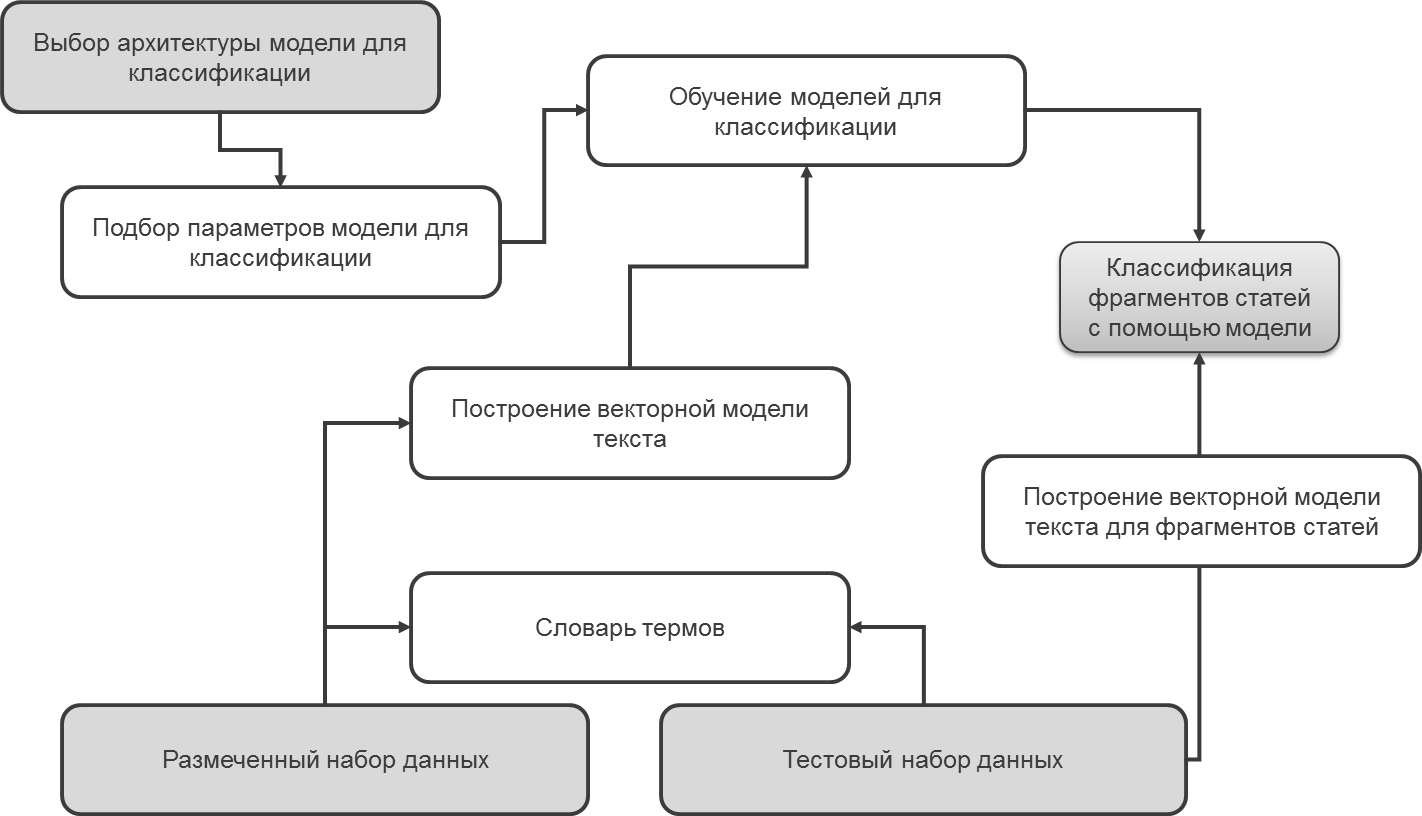
\includegraphics[width=0.8\textwidth]{op4_1}
  \label{fig:op4_1}
  \caption{ Методический каркас исследования эмоциональной окраски текстов.}
\end{figure}  

\chapter{Апробация и результаты}
%\chapter[toc version]{doc version}
\chaptermark{Апробация и результаты}
\label{chapter:experiment}

\section{Постановка эксперимента для прямой и обратной задач.}
В исследовании есть два крупных направления, которые тесно между собой переплетаются и дают комплексный, углубленный взгляд на изучаемый объект.
Перечислим эти направления: 

\begin{itemize}
\item \textit{Изучение деятельности НТЦ по внешним проявлениям.} 
К внешним проявлениям относятся цифровые артефакты деятельности организации - это опубликованные научные статьи, материалы конференций, информационные сайты в сети Интернет и новости о компании.  
Изучение цифровых артефактов производится с помощью подходов, основанных на анализе текстов и соавторов. 
\item \textit{Изучение НТЦ изнутри.} 
К исследованиям в этом направлении относятся моделирование научной деятельности, эффективность производственных процессов, самоорганизации малых творческих коллективов и модели персонала научной организации.
\end{itemize}

Допустим, что мы рассматриваем конкретную организацию с определенным
количеством сотрудников, бюджетом и планом работ. 

Нас интересуют вопросы эффективности данной организации. 
И с этой точки зрения для нас представляются важным следующие вопросы: 
\begin{itemize}
\item 
Каков интеллектуальный потенциал организации? 
Какие научные исследования организация способна выполнить самостоятельно, а какие необходимо выполнять совместно с другими научными организациями. 
Очевидно, что при выполнении совместных исследований возникают коммуникационные издержки и исследование нуждается в дополнительной координации. 
Но для эффективности важна не только принципиальная граница "может-не может", но и распределение по времени и затрачиваемым усилиям. 
\item 
Какова загруженность персонала? 
Известно, что в условиях высокой загрузки производительность деградирует.
Но для вопросов эффективности данный эффект необходимо рассматривать в динамике, так как возвращение из  деградированного к нормальному состоянию занимает определенное время.
Кроме того, важна сегментация загрузки по типам сотрудников. 
Новички могут быть как перегружены, так и недогружены работой. 
От этого зависит текучесть персонала. 
Но загрузка экспертов значительно более существено влияет на эффективность. 
Эффекты интеллектуальной усталости экспертов драматически влияют на эффективность. 
\item  
Научный задел организации истощен? 
Какова динамика создания научного задела? 
Есть ли прорывные направления в научных исследованиях, ведущихся внутри организации? 
Кто участвует в создании научного задела? 
\end{itemize}

Перечисленные параметры организации невозможно измерить.
Но от них принципиально зависит эффективность НТЦ. 
Методы оценки данных параметров разработанные автором, дают методологические подходы к прояснению поставленных выше вопросов.

Прямой метод измерения в настоящем исследованиии сводится к моделированию динамики организационной среды для получения цифровых автрфактов.
Для этого автором созданы модели персонала, модели командообразования и модели продуктивности НТЦ. 
Результатом многопрогонного эксперимента с этими моделями являются синтетические цифровые артефакты деятельности научной организации: соавторста, тематики, направления развития и др. 

Обратный метод постановки эксперимента в свою очередь анализирует реальные цифровые артефакты деятельности НТЦ. 
А именно научные статьи, материалы конференций и т.п. И на основании цифровых артефаков автор строит модель соавторства, модели научных тематик, модели научных направлений и научных школ в организации. 

\section{Модель процесса публикаций научных статей}
\label{sec:di}
В настоящем исследовании была проанализирована публикационная активность научно-технического центра ПАО ``Газпромнефть'' в электронной библиотеке OnePetro международного сообщества нефтегазовых инженеров. 
Полученная зависимость изображена на рисунке (Рис. \ref{fig:om5}).

\begin{figure}[H]
  \caption{Количество публикаций сотрудников Газпромнефть НТЦ в электронной библиотеке OnePetro и линия тренда.}
  \centering
    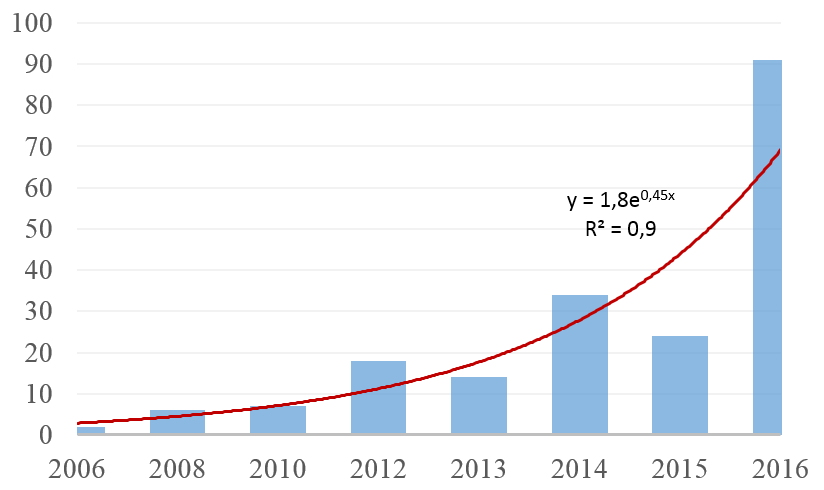
\includegraphics[width=0.8\textwidth]{om5}
  \label{fig:om5}
\end{figure}  

Экспоненциальный рост публикаций в одном издании не может продолжаться бесконечно. 
Каждое издание имеет свой предельный объем публикаций, рукописи, поступающие сверх допустимого изданием объема публикаций, повышают конкуренцию за право быть опубликованным. 
Но в результате отбора некоторые качественные рукописи отвергаются издателями.
Для изучения процесса публикации была разработана имитационная модель. 
Когнитивная карта модели процесса публикаций приведена на рисунке (Рис. \ref{fig:om6}).

\begin{figure}[H]
  \caption{Когнитивная карта модели процесса публикаций.}
  \centering
    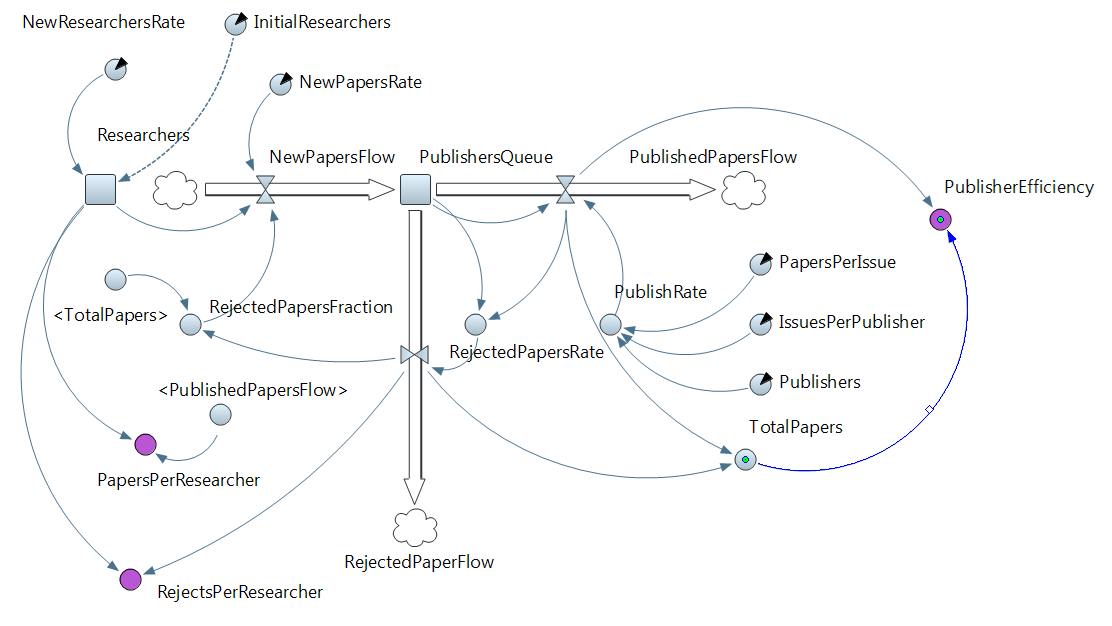
\includegraphics[width=0.8\textwidth]{om6}
  \label{fig:om6}
\end{figure} 

Созданная модель процесса публикаций содержит два накопителя:
\begin{itemize}
\tightlist
\item Researchers — исследователи,
\item PublishersQueue — очередь рукописей.
\end{itemize}

Модель управляется посредством следующих свободных параметров (Таб. \ref{tab:om3}): 

\begin{table}[H]
\centering
\caption{Свободные параметры модели процесса публикаций.}
\label{tab:om3}
\resizebox{\textwidth}{!}{%
\begin{tabular}{|l|l|}
\hline
\textbf{Название параметра} & \textbf{Описание} \\ \hline
Publishers & Количество издателей \\ \hline
PapersPerIssue & Количество статей в выпуске \\ \hline
IssuesPerPublisher & Количество выпусков на одного издателя в год \\ \hline
NewPapersRate & Скорость создания рукописей \\ \hline
InitialResearchers & Начальное количество исследователей \\ \hline
NewResearchersRate & Скорость появления новых исследователей \\ \hline
\end{tabular}%
}
\end{table}

На основании когнитивной карты модели процесса публикаций был проведен цифровой эксперимент.
На рисунке (Рис. \ref{fig:om7}) представлена зависимость эффективности публикаций от времени при различном количестве издателей.

\begin{figure}[H]
  \caption{Кривая зависимости эффективности публикаций от времени при различном количестве издателей (1,3,5,7).}
  \centering
    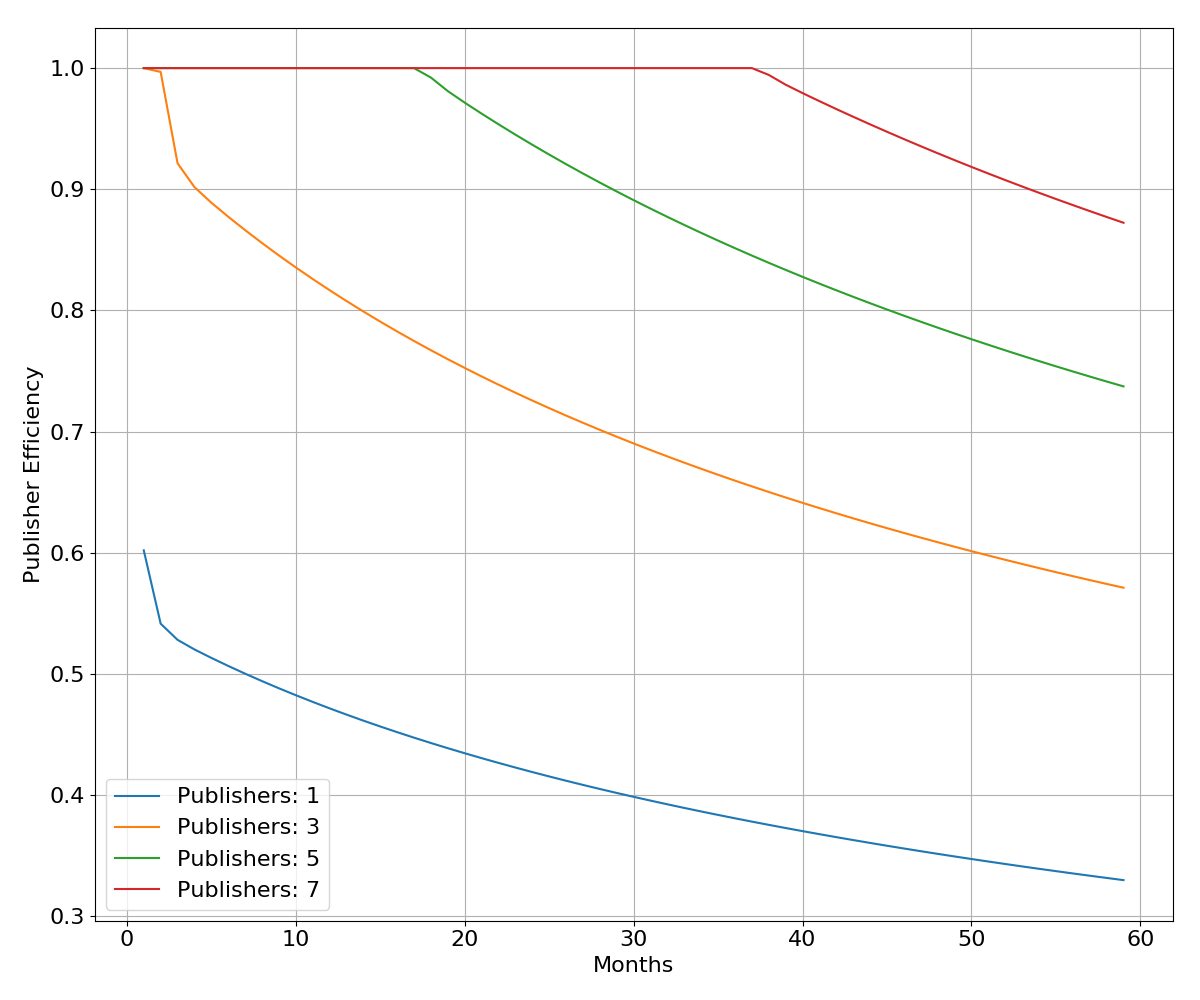
\includegraphics[width=0.8\textwidth]{om7}
  \label{fig:om7}
\end{figure} 

Падение эффективности публикаций как мы видим имеет резкий, лавинообразный характер. 
Такой характер поведения эффективности публикаций требует особого внимания, чтобы не пропустить начало стагнации и принять организационные меры для расширения количества издателей, участвующих в процессе публикации.  

Принцип разделения труда ведет к повышению эффективности процессов. 
Гипотетически расширение ролевой модели может повысить эффективность процесса публикаций. 
Независимо от количества соавторов процесс публикации определяет следующие роли: 

\begin{itemize}
\tightlist
\item Продюсер — носитель основной идеи исследования
\item Редактор — изменяет текст рукописи
\item Рецензент — диалектическая противоположность Продюсера, оппонирует, отвечает за выводы и результаты исследования
\item Переводчик — если статья не на родном языке авторов, то требуется технический перевод и вычитка
\item Специалист по работе с издателями — отвечает за поиск издателей и внешние коммуникации
\item Дизайнер — картинки, презентация для доклада
\item Докладчик — представляет результат в устном виде на конференции (если нужно и столько сколько нужно раз)
\item Исследователь данных — проведение компьютерных расчетов.
\end{itemize}

С учетом перечисленных ролей научно-исследовательская команда не изменяется.
Авторами исследования остаются именно те ученые, которые его провели. 
Повышается качество рукописи, а коммуникации становятся более профессиональными. 
Отметим, что функции внешних и внутренних корпоративных коммуникаций обычно присутствуют в организационной среде, но не имеют фокусировки на работу с индивидуальными потребностями исследователей.

\section{Измерение интеллектуального капитала НТЦ}
\label{sec:ic}
Интеллектуальный капитал (ИК) по своей природе является составным показателем продуктивности научно-исследовательской организации основным продуктом которой являются знания. В структуру ИК входят:
\begin{itemize}
\tightlist
\item Человеческий капитал 
\item Организационный капитал 
\end{itemize}

Человеческий капитал (ЧК) - включает в себя знания и навыки. 
Организационный капитал (ОК) включает в себя технологии и процессы. 
Другими словами, ЧК характеризует опыт сотрудников, а ОК характеризует то как сотрудники применяют свой опыт к поставленным задачам в данной организации. 

Помимо создания интеллектуального капитала  можно рассмотреть и его разрушение – сотрудники, которые вели исследования увольняются и уносят с собой знания.

Вклад сотрудников в интеллектуальный капитал не равнозначен. 
Далее авторы определяют роли, которые относят к ``ядру команды''. 
Потеря сотрудников, состоящих в ядре команды драматически сказывается на производительности. 
К ядру относят сотрудников с высоким уровнем опыта и наиболее востребованными в организации навыками.

Существует достаточно много подходов, описывающих жизненный цикл сотрудника внутри организации или должности , однако большинство исследований соглашается в выделении 4 основных этапов относительно уровня продуктивности:

\begin{enumerate}
\tightlist
\item начальный этап, 
\item накопление опыта, 
\item продуктивный этап, 
\item спад продуктивности.  
\end{enumerate}

При этом этап адаптации (начальный этап и накопление опыта) может отличаться в зависимости от вида деятельности и уровня позиции, но в среднем для специалистов и руководителей среднего звена занимает до полугода, около года для руководителей высшего звена.

Наибольший процент увольнений среди новичков, поэтому больше внимания необходимо уделять социальной адаптации новых сотрудников, встраиванию новичков в процессы и наставничеству.

При распаде творческой команды утечка мозгов бывает разная и не всегда наносит вред производительности. 
Другими словами, иногда уход опытного, но имеющего отличную от большинства ментальную модель сотрудника, уменьшает сдерживающие факторы роста ИК.

Существуют понятия текучести кадров ``по собственному желанию'' и ``по инициативе организации''. 
С точки зрения ИК обе составляющие имеют негативное влияние. 
В Российской практике сложилось устойчивое понятие ``текучести кадров'': показатель, фиксирующий уровень изменения состава вследствие увольнения и перехода на другую работу по личным мотивам. 
В понятие текучести обычно не включают переход сотрудника к другому работодателю через перевод, что сильно искажает российские результаты по сравнению с иностранными. В разных индустриях и сферах промышленности, а также на разных уровнях управления ``нормой'' считают различные значения текучести персонала (от 2-5 до 80\%), что обусловлено особенностями бизнеса и категориями сотрудников. 
Так, например, для розничной торговли и массовой сферы обслуживания характерны самые высокие показатели, тогда как для тяжелой промышленности в целом нормальные достаточно низкие значения (5-10\%).
В целом, можно отметить, что уровень текучести повышается по мере выхода на работу более молодых поколений Х, Y.

Важно так же отметить связь выгорания, усталости и текучести персонала, что имеет негативное воздействие на продуктивность организации.
Положительной обратной связью обладают текучесть кадров и уменьшение производительности труда. 
Организации с высокой текучестью кадров обычно испытывают больше проблем с производительностью труда и с накоплением ИК. 

Наиболее значимой составляющей ИК является продуктивность организации, отражающая отношение эффективного персонала к общему числу сотрудников.  

Автор данного исследования построил модель ИК на основе продуктивности организации. 
Для этого была создана модель численности персонала. 
Модель численности обычно решает задачи прогнозирования численности персонала в зависимости от определенных драйверов численности, как правило, внешних (количество проектов, задач, клиентов, объектов обслуживания) на основе, текущей или заданной производительности труда.
Основной проблемой моделей численности, разрабатываемых организациями, является линейные зависимости численности от драйверов и отсутствие учета фактора адаптации персонала (то есть перехода от новичков к опытным сотрудникам), а также применимость только в конкретной организации с ее драйверами/процессами.

Задачей данного эксперимента является рассмотрение поведения ИК в условиях нагрузки на персонал. 
Для оценки изменений ИК в условиях нагрузки была создана модель выполнения заданий. 
Обе модели в отдельности и общая модель ИК, построенная ни их взаимодействии описаны далее. 

На рисунке (Рис.\ref{fig:icmon1}) приведена когнитивная карта модели численности персонала, разработанная автором данного исследования по рекомендациям из \cite{oliva2010d} .

\begin{figure}[H]
  \caption{Когнитивная карта модели численности персонала.}
  \centering
    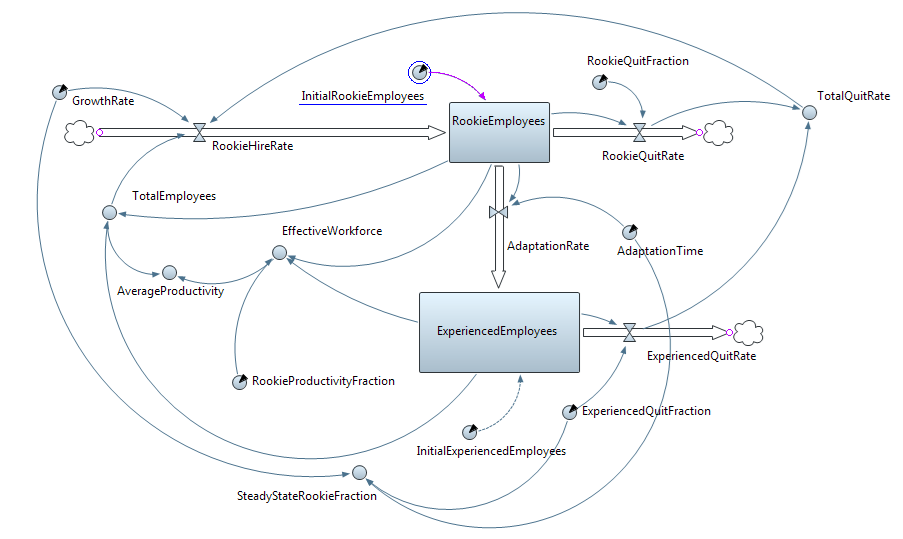
\includegraphics[width=0.8\textwidth]{icmon1}
  \label{fig:icmon1}
\end{figure}  

Модель численности персонала состоит из двух накопителей – Rookie Employees (Новички) и Experienced Employees (Опытные сотрудники) и четырех потоков: 

\begin{itemize}
\tightlist
\item Набор новичков (RookieHireRate),
\item Увольнение новичков (RookieQuitRate),
\item Адаптация новичков в опытных сотрудников (AdaptationRate),
\item Увольнение опытных сотрудников (ExperiencedQuitRate).
\end{itemize}

Свободные параметры модели численности персонала приведены в таблице \ref{tab:icmon1}: 

\begin{table}[H]
\centering
\caption{Свободные параметры модели численности персонала.}
\label{tab:icmon1}
\resizebox{\textwidth}{!}{%
\begin{tabular}{|l|l|l|}
\hline
\textbf{Название параметра} & \textbf{Обозначение параметра} & \textbf{Значение параметра} \\ \hline
Скорость набора персонала & Growth Rate & 0.01 в неделю (от Total Employees) \\ \hline
Начальное количество новичков в компании & Initial Rookie Employees & 40 человек \\ \hline
Начальное количество опытных сотрудников в компании & Initial Experienced Employees & 60 человек \\ \hline
Время адаптации новичка в опытного сотрудника & Adaptation Time & 50-100 недель \\ \hline
Доля вклада новичка в продуктивность персонала & Rookie Productivity Fraction & 30-80\% \\ \hline
Доля увольнений новичков & Rookie Quit Rate & 0.01 \\ \hline
Доля увольнений опытных сотрудников & Experienced Quit Fraction & 0.004 \\ \hline
\end{tabular}%
}
\end{table}

Динамические переменные модели численности персонала перечислены в Таблице Таб. \ref{tab:icmon2}: 

\begin{table}[H]
\centering
\caption{Динамические переменные модели численности персонала }
\label{tab:icmon2}
\resizebox{\textwidth}{!}{%
\begin{tabular}{|l|l|l|}
\hline
\textbf{Название переменной} & \textbf{Обозначение} & \textbf{Формула} \\ \hline
Общее количество сотрудников & Total Employees & RookieEmployees+ExperiencedEmployees \\ \hline
Эффективное количество сотрудников & Effective Workforce & ExperiencedEmployees + RookieProductivityFraction * RookieEmployees \\ \hline
Средняя продуктивность & Average Productivity & EffectiveWorkforce / TotalEmployees \\ \hline
Устойчивая доля новичков & Steady State Rookie Fraction & AdaptationTime*(ExperiencedQuitFraction+GrowthRate)/(1+AdaptationTime*(ExperiencedQuitFraction+GrowthRate)) \\ \hline
Скорость увольнений & Total Quit Rate & RookieQuitRate+ExperiencedQuitRate \\ \hline
\end{tabular}%
}
\end{table}

Потоки перечисленные выше вычисляются по формулам, приведенным в Таблице  \ref{tab:icmon3}: 

\begin{table}[H]
\centering
\caption{Формулы потоков модели численности персонала.}
\label{tab:icmon3}
\resizebox{\textwidth}{!}{%
\begin{tabular}{|l|l|}
\hline
\textbf{Название потока} & \textbf{Формула} \\ \hline
Набор новичков & RookieHireRate = TotalQuitRate + TotalEmployees*GrowthRate \\ \hline
Увольнение новичков & RookieQuitRate = RookieEmployees*RookieQuitFraction \\ \hline
Адаптация новичков в опытных сотрудников & AdaptationRate = RookieEmployees/AdaptationTime \\ \hline
Увольнение опытных сотрудников & ExperiencedQuitRate = ExperiencedEmployees*ExperiencedQuitFraction \\ \hline
\end{tabular}%
}
\end{table}

Для моделирования нагрузки модель численности персонала может быть дополнена процессами выполнения заданий. 
На Рис. \ref{fig:icmon2}  приведена когнитивная карта модели выполнения заданий, разработанная авторами данного исследования.

\begin{figure}[H]
  \caption{Когнитивная карта модели выполнения заданий.}
  \centering
    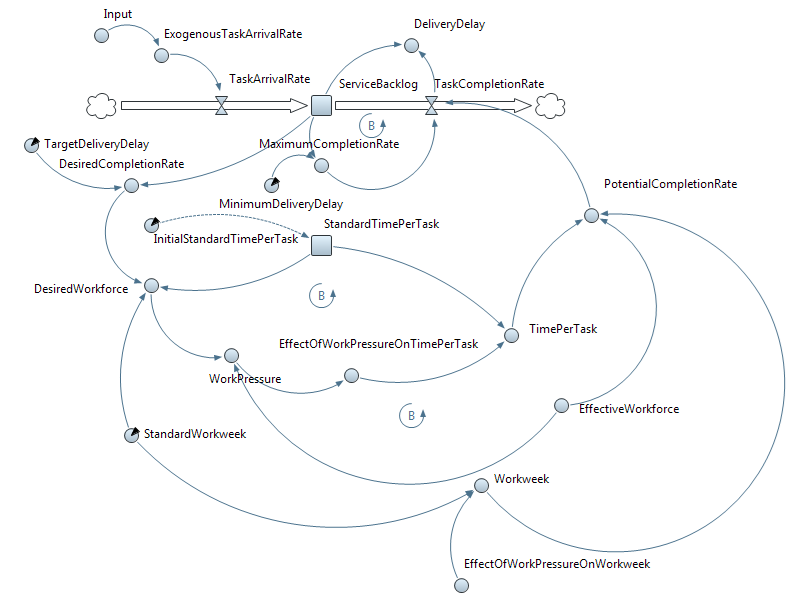
\includegraphics[width=0.8\textwidth]{icmon2}
  \label{fig:icmon2}
\end{figure}  

Модель выполнения заданий состоит из двух накопителей: ServiceBacklog (очередь заданий) и StandardTimePerTask (Стандартное время на выполнение задания). 
Модель выполнения заданий управляется свободными параметрами, приведенными в Таблице \ref{tab:icmon4}:

\begin{table}[H]
\centering
\caption{Свободные параметры модели выполнения заданий.}
\label{tab:icmon4}
\resizebox{\textwidth}{!}{%
\begin{tabular}{|l|l|l|}
\hline
\textbf{Название параметра} & \textbf{Обозначение параметра} & \textbf{Значение параметра} \\ \hline
Стандартная рабочая неделя & Standard Workweek & 40 часов \\ \hline
Целевая задержка исполнения задания & Target Delivery Delay & 0.2 недель \\ \hline
Начальное время выполнения задания & Initial Standard Time Per Task & 1 человек*час/задание \\ \hline
Минимальная задержка выполнения задания & Minimum Delivery Delay & 0.05 недель \\ \hline
\end{tabular}%
}
\end{table}

Динамические переменные модели выполнения заданий приведены в Таблице \ref{tab:icmon5}:

\begin{table}[H]
\centering
\caption{Динамические переменные модели выполнения заданий.}
\label{tab:icmon5}
\resizebox{\textwidth}{!}{%
\begin{tabular}{|l|l|l|}
\hline
\textbf{Название переменной} & \textbf{Обозначение} & \textbf{Формула} \\ \hline
Необходимое количество сотрудников & Desired Workforce & DesiredCompletionRate * StandardTimePerTask / StandardWorkweek \\ \hline
Потенциальная скорость выполнения заданий & Potential Completion Rate & EffectiveWorkforce * Workweek / TimePerTask \\ \hline
Время затраченное на выполнение задания & Time Per Task & StandardTimePerTask * EffectOfWorkPressureOnTimePerTask(WorkPressure) \\ \hline
Требуемая скорость выполнения заданий & Desired Completion Rate & ServiceBacklog / TargetDeliveryDelay \\ \hline
Степень нагрузки на персонал & WorkPressure & DesiredWorkforce / EffectiveWorkforce \\ \hline
Рабочая неделя & Workweek & StandardWorkweek * EffectOfWorkPressureOnWorkweek(WorkPressure) \\ \hline
\end{tabular}%
}
\end{table}

Очередь заданий (ServiceBacklog) управляется экзогенной динамическим потоком поступления новых заданий (TaskArrivalRate) и потоком выполненных заданий (TaskCompletionRate). 
Точка равновесия для модели выполнения заданий  определена следующим уравнением (\ref{eq:icmon1}):

\begin{equation}
EffectiveWorkforce = Desired Workforce
\label{eq:icmon1}
\end{equation}

Модель численности персонала представляет основу для модели выполнения заданий. 
Вместе эти модели представляют динамику навыков и процессов, что характеризует интеллектуальный капитал организации, как мы уже отмечали ранее.
Модели соединены динамическими переменными, приведенными в Таблице \ref{tab:icmon6}:

\begin{table}[H]
\centering
\caption{Динамические переменные, объединяющие модель численности персонала и модель выполнения заданий.}
\label{tab:icmon6}
\resizebox{\textwidth}{!}{%
\begin{tabular}{|l|l|l|}
\hline
\textbf{Название переменной} & \textbf{Обозначение} & \textbf{Описание действия} \\ \hline
Эффективное количество сотрудников & Effective Workforce & Вычисляется в модели численности персонала для модели выполнения заданий. Описывает количество сотрудников для выполнения заданий. \\ \hline
Рабочая неделя & Workweek & Вычисляется в модели выполнения заданий для модели численности персонала. Описывает количество часов требуемых для выполнения поступающих заданий. \\ \hline
\end{tabular}%
}
\end{table}

Для выявления поведения ИК исследуем кривые производительности. 
Кривая производительности является графическим представление изменения скорости обучения определённому виду деятельности. 
На рисунке \ref{fig:icmon3} приведены кривые производительности для модели численности персонала при различных значениях времени адаптации новичков. 
В модели численности персонала динамической переменной, характеризующей производительности, является Средняя продуктивность персонала (Average Productivity).

\begin{figure}[H]
  \caption{Кривые производительности для различных значений Времени адаптации новичков.}
  \centering
    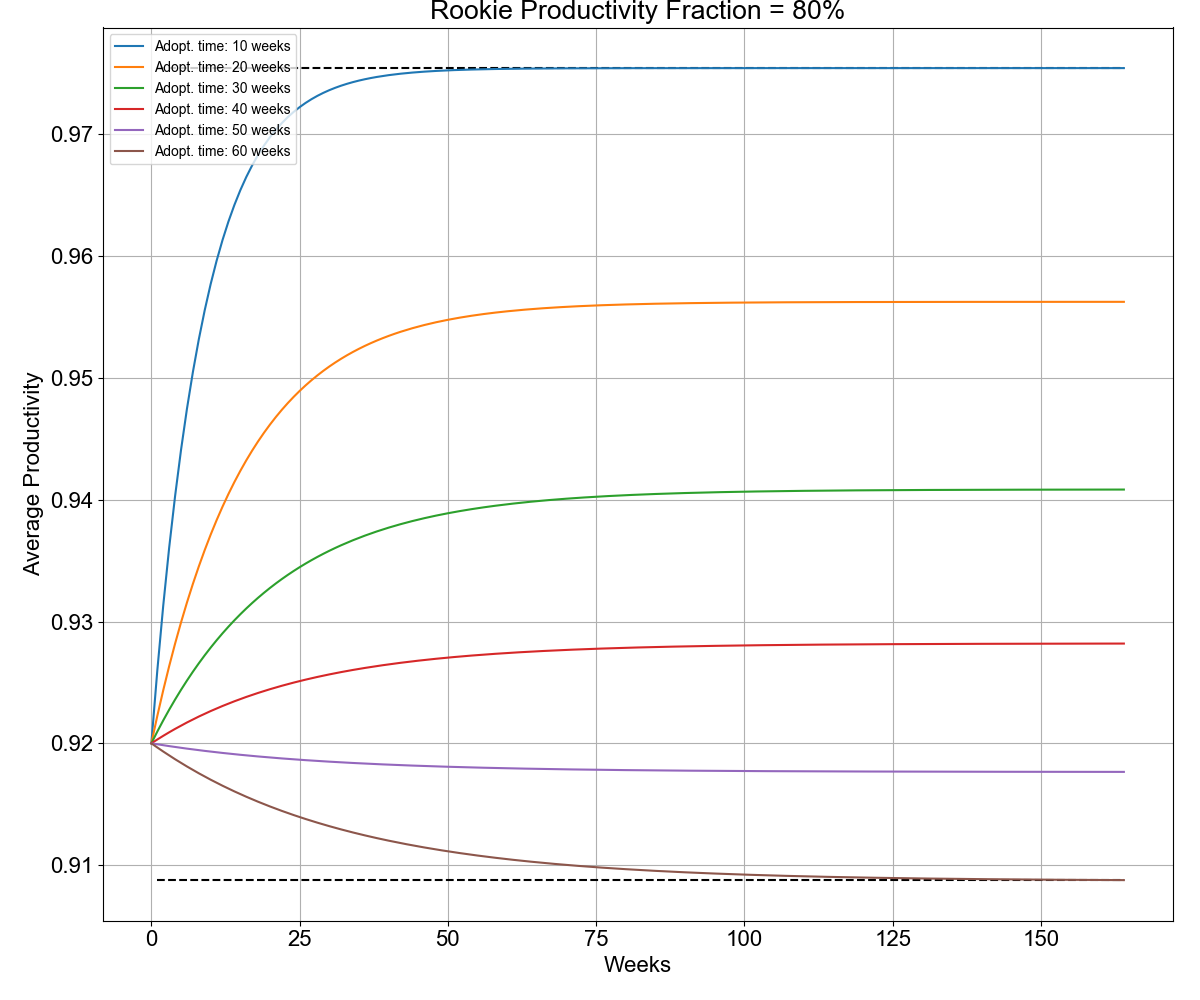
\includegraphics[width=0.8\textwidth]{icmon3}
  \label{fig:icmon3}
\end{figure}  

Как мы видим из рисунка \ref{tab:icmon3} для Доли вклада новичка равной 80\% при временах адаптации более 50 недель кривая обучаемость стремиться к нижней асимптоте, а при временах более 60 недель стремиться к верхней асимптоте Средней продуктивности. 
Таким образом, демонстрируя разный характер поведения. 
На практике это означает, что при значительном времени адаптации новичков организационная производительность падает, так как количество опытных сотрудников в коллективе уменьшается по отношению к новичкам, а вклад в продуктивность от новичков меньше чем от опытных сотрудников. 

С другой стороны, из кривых на рисунке \ref{fig:icmon4} видно, что для Времени адаптации равному 20 неделям кривые продуктивности имеют единый характер и отличаются скоростью выхода на предельное значение – асимптоту. 

\begin{figure}[H]
  \caption{Кривые производительности для различных значений Доли вклада новичков.}
  \centering
    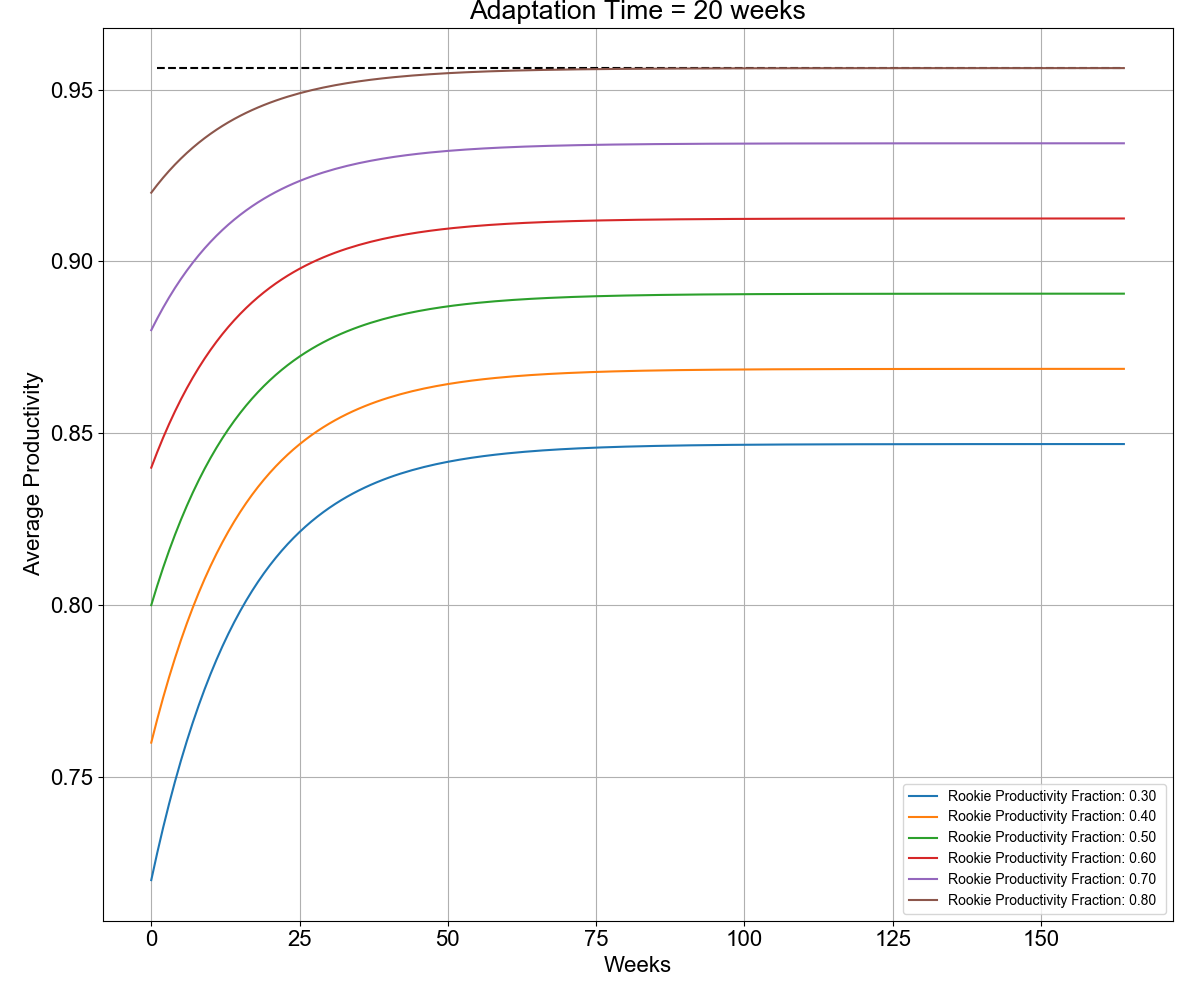
\includegraphics[width=0.8\textwidth]{icmon4}
  \label{fig:icmon4}
\end{figure} 

Небольшие Доли вклада новичков означают, что сложность заданий не подразумевает участия в них неподготовленных сотрудников. 
С другой стороны, большие Доли вклада новичков означают, что задания позволяют даже неопытному сотруднику работать с высокой отдачей, приближающейся к отдачи опытных сотрудников.

Для моделирований ИК под нагрузкой мы будем использовать экзогенную функцию для потока заданий (Рис. \ref{fig:icmon5}), для создания разных нагрузок.

\begin{figure}[H]
  \caption{Кривые производительности и нагрузки для модели ИК.}
  \centering
    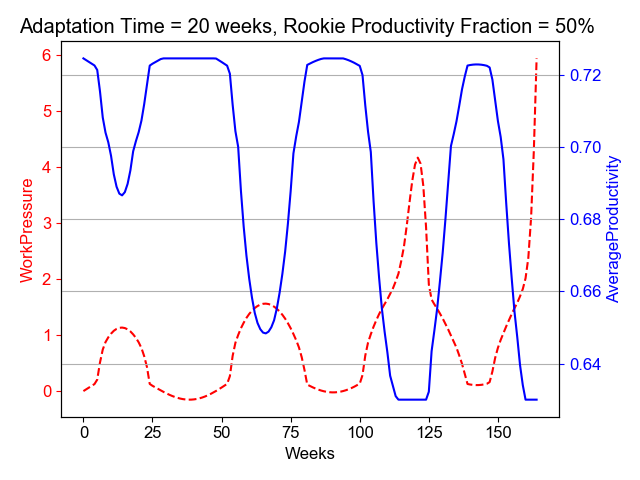
\includegraphics[width=0.8\textwidth]{icmon5}
  \label{fig:icmon5}
\end{figure} 

Из рисунка \ref{fig:icmon5} мы видим, что в пиковых нагрузках производительность падает, но за счет адаптации новичков организация, восстанавливает производительность, когда нагрузка спадает. 
Для различных времен адаптации в модели ИК кривые производительности будут иметь вид, представленный на рисунке (Рис. \ref{fig:icmon6}).

\begin{figure}[H]
  \caption{Кривые производительности для различных значений Времени адаптации новичков с учетом нагрузки.}
  \centering
    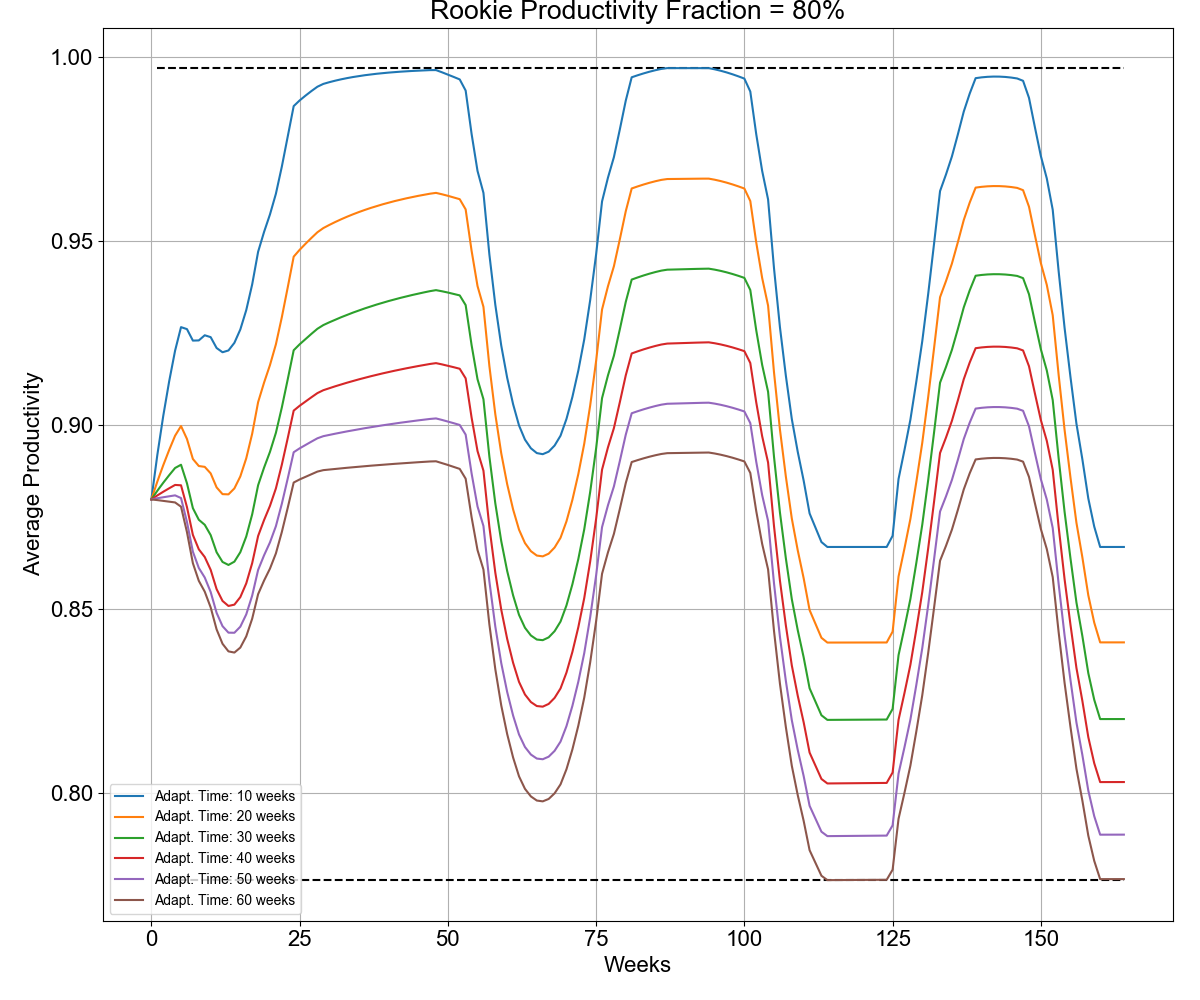
\includegraphics[width=0.8\textwidth]{icmon6}
  \label{fig:icmon6}
\end{figure} 

На рисунке (Рис.\ref{fig:icmon7})  представлены кривые производительности для Времени адаптации равному 20 неделям с учетом нагрузки. 
Мы можем наблюдать различное поведение производительности до выхода на асимптоты при различных долях участия новичков, что отражает тот факт, что возможное включении новичков в решение заданий (до адаптации) характеризует эти задания, как достаточно простые и типовые.

\begin{figure}[H]
  \caption{Кривые производительности для различных значений Доли вклада новичков с учетом нагрузки.}
  \centering
    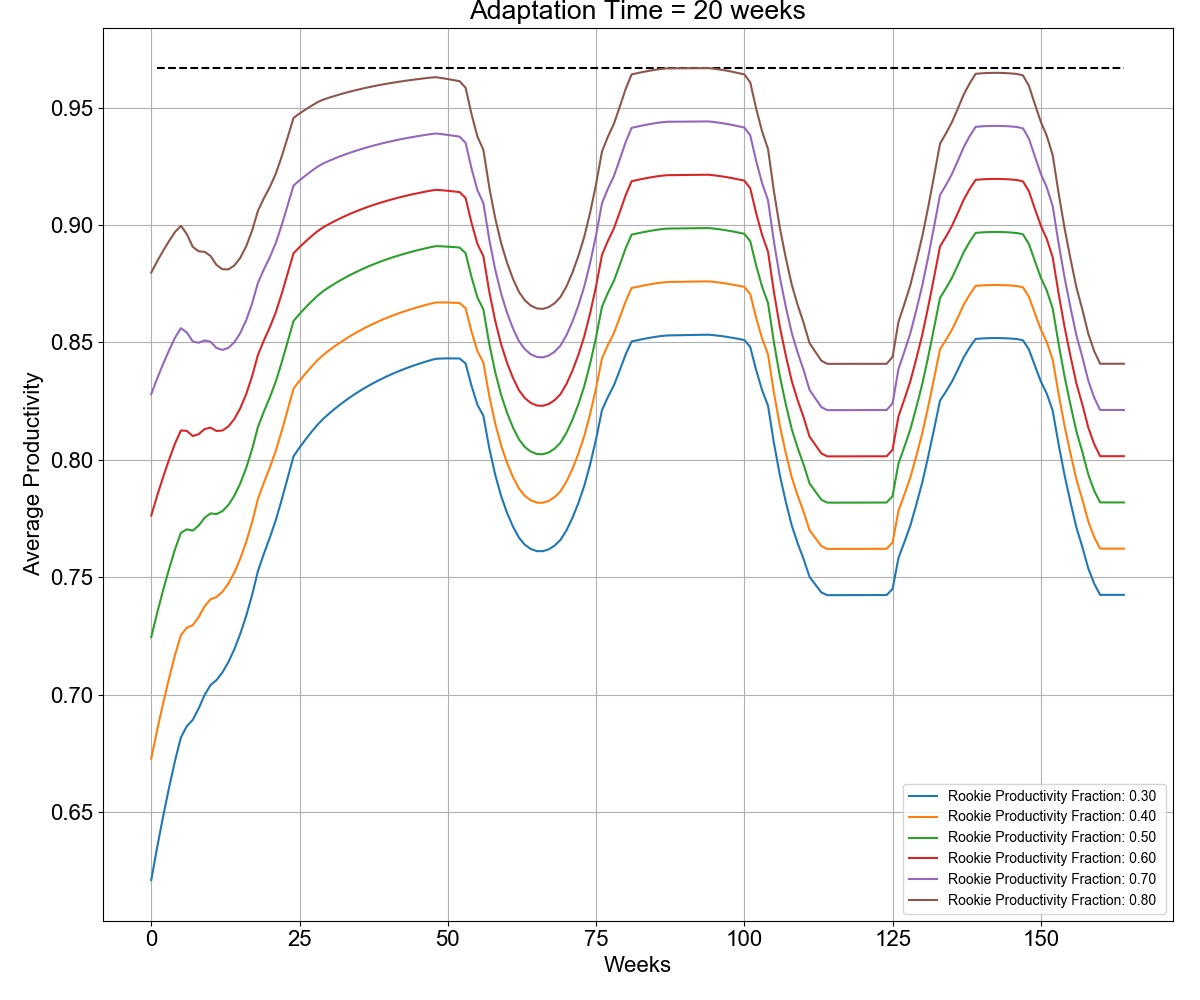
\includegraphics[width=0.8\textwidth]{icmon7}
  \label{fig:icmon7}
\end{figure} 

Отметим, что при небольшом времени адаптации новичков (20 недель) и высокой доли участия новичков в продуктивности (80\%) относительное падение продуктивности ниже, чем при невысокой высокой доли участия новичков в продуктивности (30\%). 
Это наблюдение подтверждает тот факт, что при возрастании нагрузки коротких и простых заданий для новичков их продуктивность падает меньше, чем на сложных заданиях.

Для моделирования эффекта ``выгорания'' и ``усталости'' сотрудников в условиях длительной работы в режиме удлинённой недели в модель ИК введены следующие зависимости: 
\begin{enumerate}
\tightlist
\item Эффект ``выгорания'' состоит в увеличении скорости увольнения опытных сотрудников в зависимости от времени работы в условиях удлинённой недели.
\item Эффект ``усталости'' сотрудников состоит в уменьшении производительности сотрудников в зависимости от времени работы в условиях удлинённой недели.
\end{enumerate}

На рисунке (Рис.\ref{fig:icmon8})  изображен результат симуляции модели ИК для 500 недель. Такой длительный срок выбран с целью показать эффекты ``выгорания'' и ``усталости'' персонала и как следствие падение продуктивности вызванной работой в условиях удлинённой рабочей недели.

\begin{figure}[H]
  \caption{Кривые производительности и нагрузки для модели ИК в условиях удлинненой рабочей недели.}
  \centering
    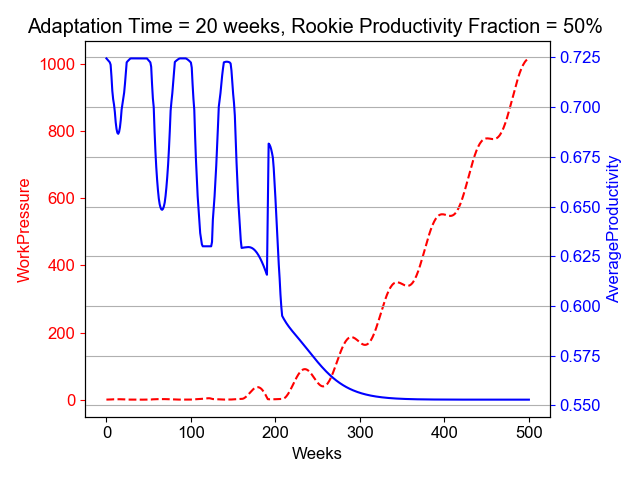
\includegraphics[width=0.8\textwidth]{icmon8}
  \label{fig:icmon8}
\end{figure} 

Падение производительности, вызванное длительной высокой нагрузкой, драматически влияет на ИК. 
В заключение на рисунке (Рис.\ref{fig:icmon9}) представлены кривые изменения человеческого капитала – опытных сотрудников, новичков и общего числа сотрудников. Отдельно приведена кривая требуемого количества сотрудников для выполнения поступающих заданий. 
Мы видим, что количество новичков растет быстрее, чем количество опытных сотрудников.

\begin{figure}[H]
  \caption{Кривые изменения человеческого капитала по модели ИК.}
  \centering
    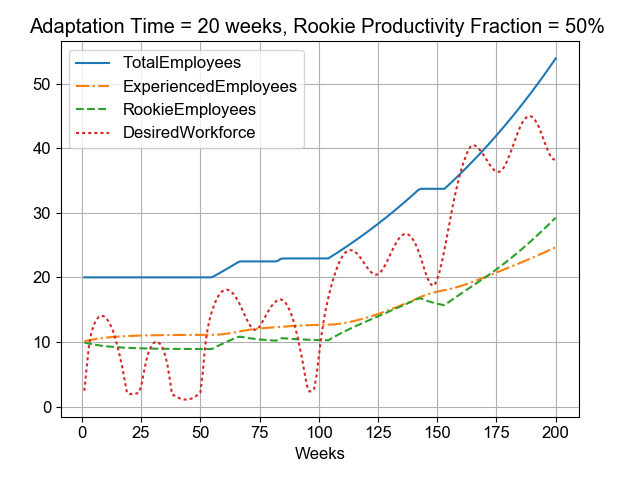
\includegraphics[width=0.8\textwidth]{icmon9}
  \label{fig:icmon9}
\end{figure} 

Приведенные результаты эксперимента подтверждает теоретические работы по изучению процессов управления интеллектуальным капиталом. 
Новизна данного исследования состоит в выработке количественных оценок, помогающих уточнить стратегию управления интеллектуальным капиталом научно-исследовательской организации. 

Рассмотренная автором ситуация работы в условиях высокой нагрузки является типичной для российской экономики в современных условиях и особенно актуально в нефтегазовой отрасли.

\section{Результаты моделирования командообразования в научной деятельности}
\label{sec:so}
Допустим, что в отраслевой научно-исследовательской организации $\Omega$  работают лаборатории $\lambda_i$ , где $i \in (1 \dots N_{\lambda})$ . 
Обозначим множество лабораторий $ \Lambda = \{ \lambda_i, \dots , \lambda_{N_{\Lambda}} \}$.
В лабораториях работают научные сотрудники $ A = \{ a_{i}, \dots, a_{N_A} \} $.  

Обозначим множество тематик $t_i$, где $i \in (1, \dots, N_T )$, по которым организация $\Omega$ ведет НИР как $T = \{ t_1, \dots , t_{N_T} \}$. Тогда деятельность организации $\Omega$ по выполнению НИР может быть описана следующими компонентами (\ref{eq:so1}):
\begin{equation} 
\label{eq:so1}
\mathbb{M}_{\Omega} = \bigg \{ S, \Xi, \Psi, E \bigg \} \mbox {, где}  S = \{ \Lambda, A, T, P, X \}
\end{equation} 

Помимо вышеопределенных компонент в уравнении \ref{eq:so1} присутствуют:

\begin{itemize}
\item $ \Xi = \{ \xi_1 , \dots , \xi_{N_{\Xi}} \} $ -- множество связей между субъектами (знакомство, соавторство и др.),
\item $ \Psi = \{ \psi_1 , \dots , \psi_{N_{\Psi}} \} $ -- множество действий субъектов (``поиск темы'', ``отправка тезисов'' и др.),
\item $ P = \{ \rho_1 , \dots , \rho_{N_P} \} $ -- множество научных работ,
\item $ X = \{ \chi_1 , \dots , \chi_{N_X}  \} $ -- множество научных журналов и конференций.
\end{itemize}

Сотрудники  организации $\Omega$  выполняют НИР по тематикам $T$ , создают научные статьи и доклады $P$ для публикации их в журналах и выступлениях на конференциях $X$.
При создании научных статей $P$ используются обзоры материалов журналов и конференций $X$.
Конференции и редакции журналов $X$ устанавливают приоритетные тематики $T$ и принимают статьи для публикации по определенному графику (тезисы, полный текст, замечания рецензентов, выступление, публикация) и от наиболее квалифицированных и опытных научных работников.
Научный работник обладает квалификациями по тематикам $T$, которые можно представить в виде n-мерного вектора $(c_1, \dots , c_{N_T} )$ и опытом написания статей $(e_1 , \dots , e_{N_E} )$, где $c_i,e_i \in \mathbb{R}$. 
И квалификации, и опыт не нуждаются в нормировке. 
Квалификация растет при успешном выполнении НИР, а опыт растет с успешной публикацией статей по соответствующей тематике.
Имитационное моделирование представляет собой статистический эксперимент. 
Его результаты должны основываться на соответствующих статистических проверках. 
Автор выбрал метод повторения для вычисления доверительных интервалов и проверки гипотез.
Таким образом, каждое наблюдение представляется независимым прогоном модели, в котором переходный период не учитывается.
Далее производится вычисление средних величин выборки. 
Так как, прогоны независимы, то применяется стандартная формула для дисперсии.
Преимуществом данного метода является то, что каждый имитационный прогон модели определяется своей последовательностью случайных чисел из интервала [0;1], что действительно обеспечивает статистическую независимость получаемых наблюдений. 
Недостатком является то, что все наблюдения могут оказаться под сильным влиянием начальных переходных условий.

В качестве калибровки для моделирования взят Газпромнефть НТЦ. 
В рамках НТЦ выбраны шесть тематик исследований $T = \{ t_1, \dots , t_{N_T} \} $ , где $N_T = 6 $ :

\begin{enumerate}
\tightlist
\item Разработка и эксплуатация нефтяных месторождений
\item Геология и геологоразведочные работы
\item Информационные технологии
\item Техника и технология добычи нефти
\item Проектирование обустройства месторождений
\item Бурение скважин
\end{enumerate}

В качестве издателя $\chi_1$ выбрана редакция ``Нефтяное хозяйство'' выпускающая одноименный журнала с 1933 года. Авторы выбрали номер журнала за декабрь 2016 (НХ,12-2016), полностью состоящий из статей сотрудников ``Газпромнефть НТЦ''. В качестве конференции $\chi_2$ выбрана конференция 16RPTC (SPE Russian Petroleum Technology Conference and Exhibition), прошедшая 24 октября 2016 года в Москве. 
Таким образом, $X = \{ \chi_1, \dots , \chi_{N_X} \} $ , где $ N_{X} = 2$.

В настоящее время в анализе социальных коллабораций выделяются два подхода:
\begin{itemize}
\tightlist
\item Структурный подход акцентирует внимание на геометрической форме сети и интенсивности взаимодействий (весе ребер). Для интерпретации результатов в данном случае используются структурные теории и теории сетевого обмена.
\item Динамический подход акцентирует внимание на изменениях в сетевой структуре с течением времени
\end{itemize}

Целью эксперимента  на данном этапе было подтвердить достаточность структуры компонент модели $\mathbb{M}_{\Omega}$ на примере научно-технического центра из нефтегазовой отрасли. При наблюдении визуализации поведения агентов у авторов не возникло необходимости в добавлении новых компонентов в модель.

Для поставленных условий на основании $\mathbb{M}_{\Omega}$ была создана частная модель $\mathbb{M}_{GPN}$  и проведена много прогонная симуляция модели (Рис. \ref{fig:so1}).

\begin{figure}[H]
  \caption{Фрагмент визуализации прогона симуляции частной модели для НТЦ из нефтегазовой отрасли.}
  \centering
    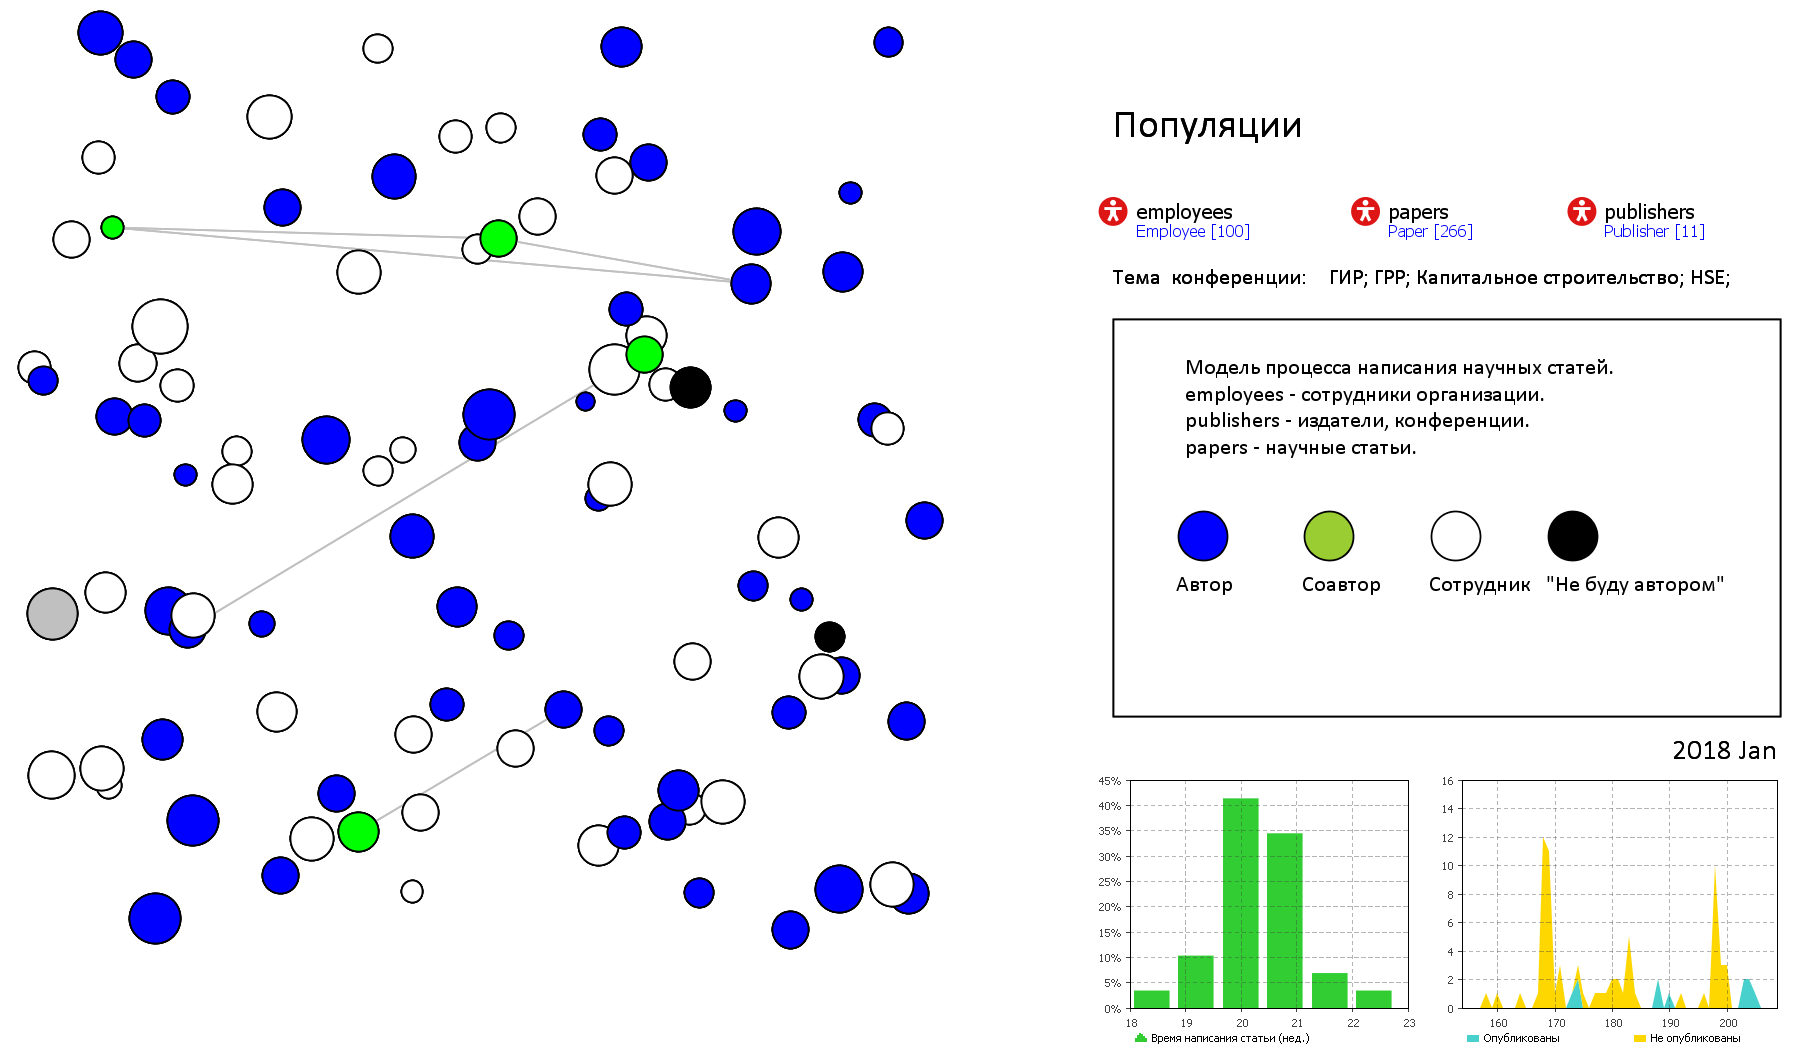
\includegraphics[width=0.8\textwidth]{so1}
  \label{fig:so1}
\end{figure}  

Далее на основании симуляций была создана база данных для последующего исследования процессов.
База данных содержит следующие основные сущности (Рис. \ref{fig:so2}).

\begin{figure}[H]
  \caption{Entity relationship diagram (ERD): Сущности процесса создания научных статей.}
  \centering
    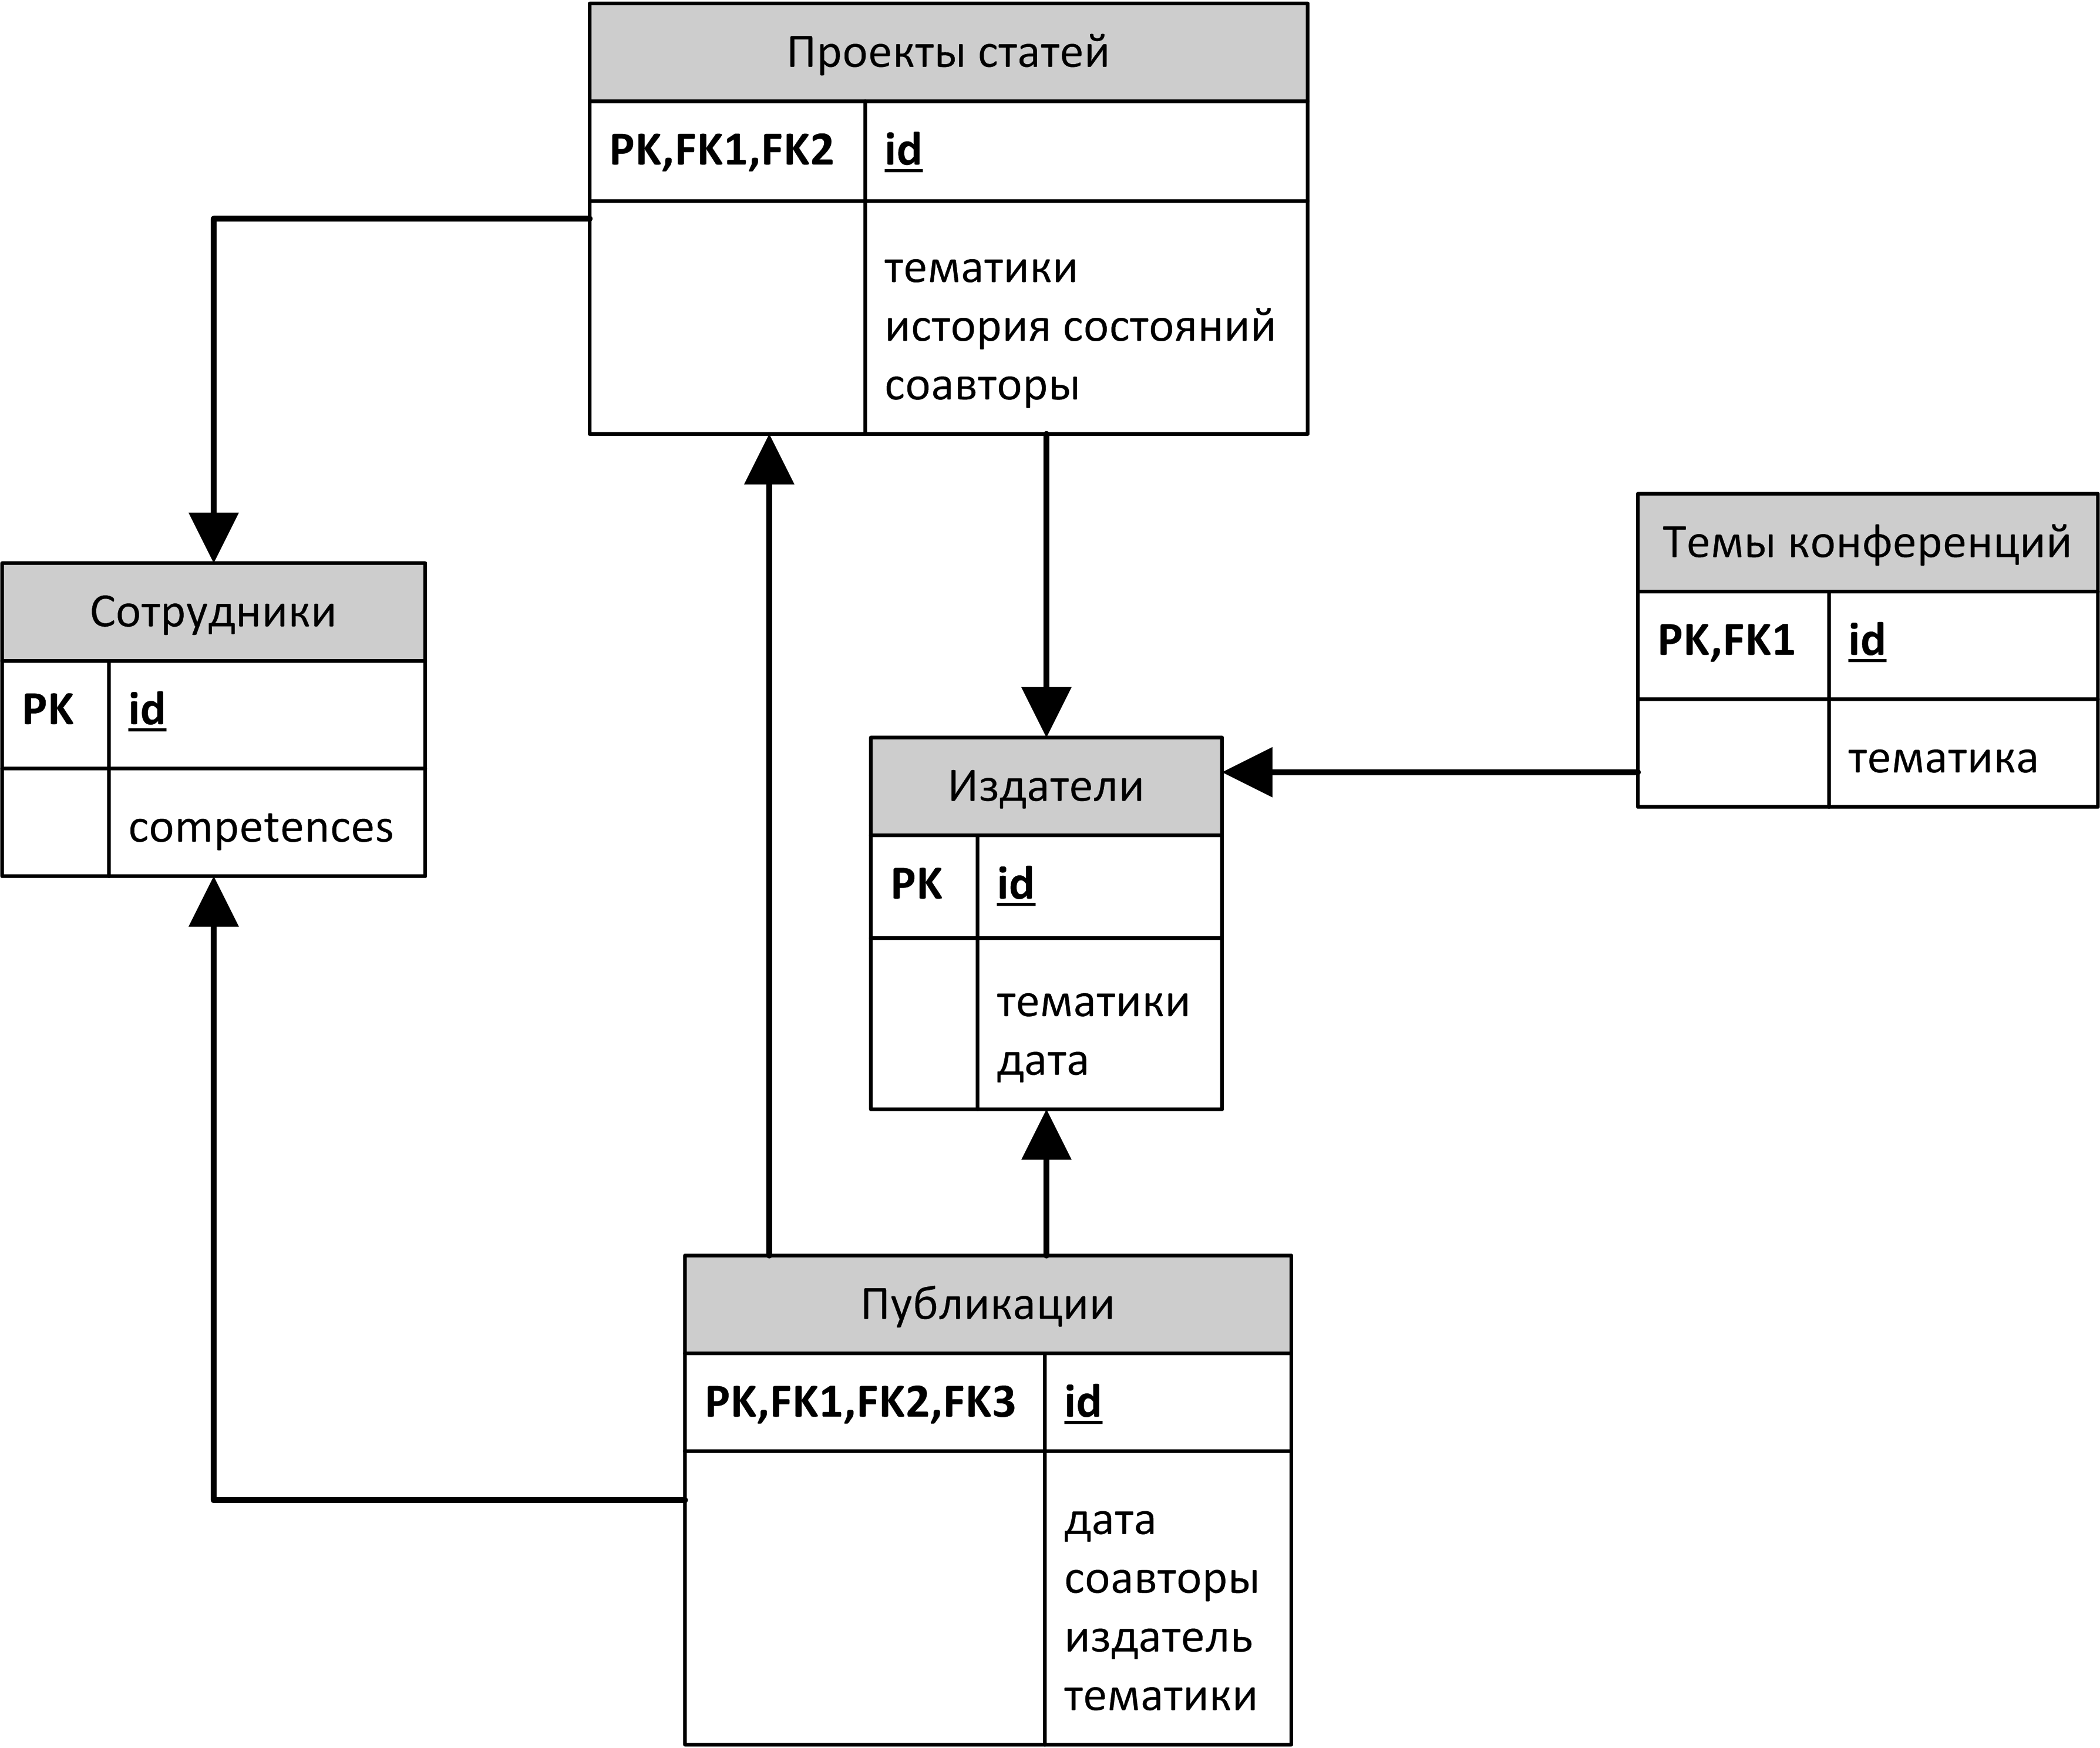
\includegraphics[width=0.8\textwidth]{so2}
  \label{fig:so2}
\end{figure}  

По результатам имитационного моделирования нами были получены следующие результаты для процесса создания и публикации научной статьи:
\begin{enumerate}
\item Среднее время написания статьи: $20 \pm 2$ недель.
\item Среднее число соавторов: $3.5 \pm 1.0$
\item Максимальное число соавторов: $7 \pm 3$
\item Среднее количество статей на одного автора в год: $2 \pm  0.5$
\item Доля статей, не уложившихся в график публикации: $40 \pm 10$ \%.
\end{enumerate}

Данные результаты находятся в согласии с опытом автора, но нуждаются в дальнейшей проверке.
Для оценки корректности результатов моделирования было проведено сопутствующее библиометрическое исследование реальных эмпирических данных по собственной методике автора \cite{KDGY}. 
В соответствии с поставленными условиями эксперимента была создана база публикаций, содержащая следующие информационные поля:

\begin{enumerate}
\tightlist
\item Дата публикации статьи
\item Список авторов
\item Название статьи
\item Тематика статьи согласно классификатору тематик $T$
\item Издатель согласно классификатору $X$
\end{enumerate}

В базу публикаций были собраны статьи издательства ``Нефтяное хозяйство'' и публикации из электронной библиотеки сообщества нефтегазовых инженеров SPE OnePetro, сделанные сотрудниками Газпромнефть НТЦ.
Проведен анализ публикаций и построен граф соавторств (Рис.\ref{fig:so3}).

\begin{figure}[H]
  \caption{Синтетический граф соавторств для НТЦ "Газпромнефть".}
  \centering
    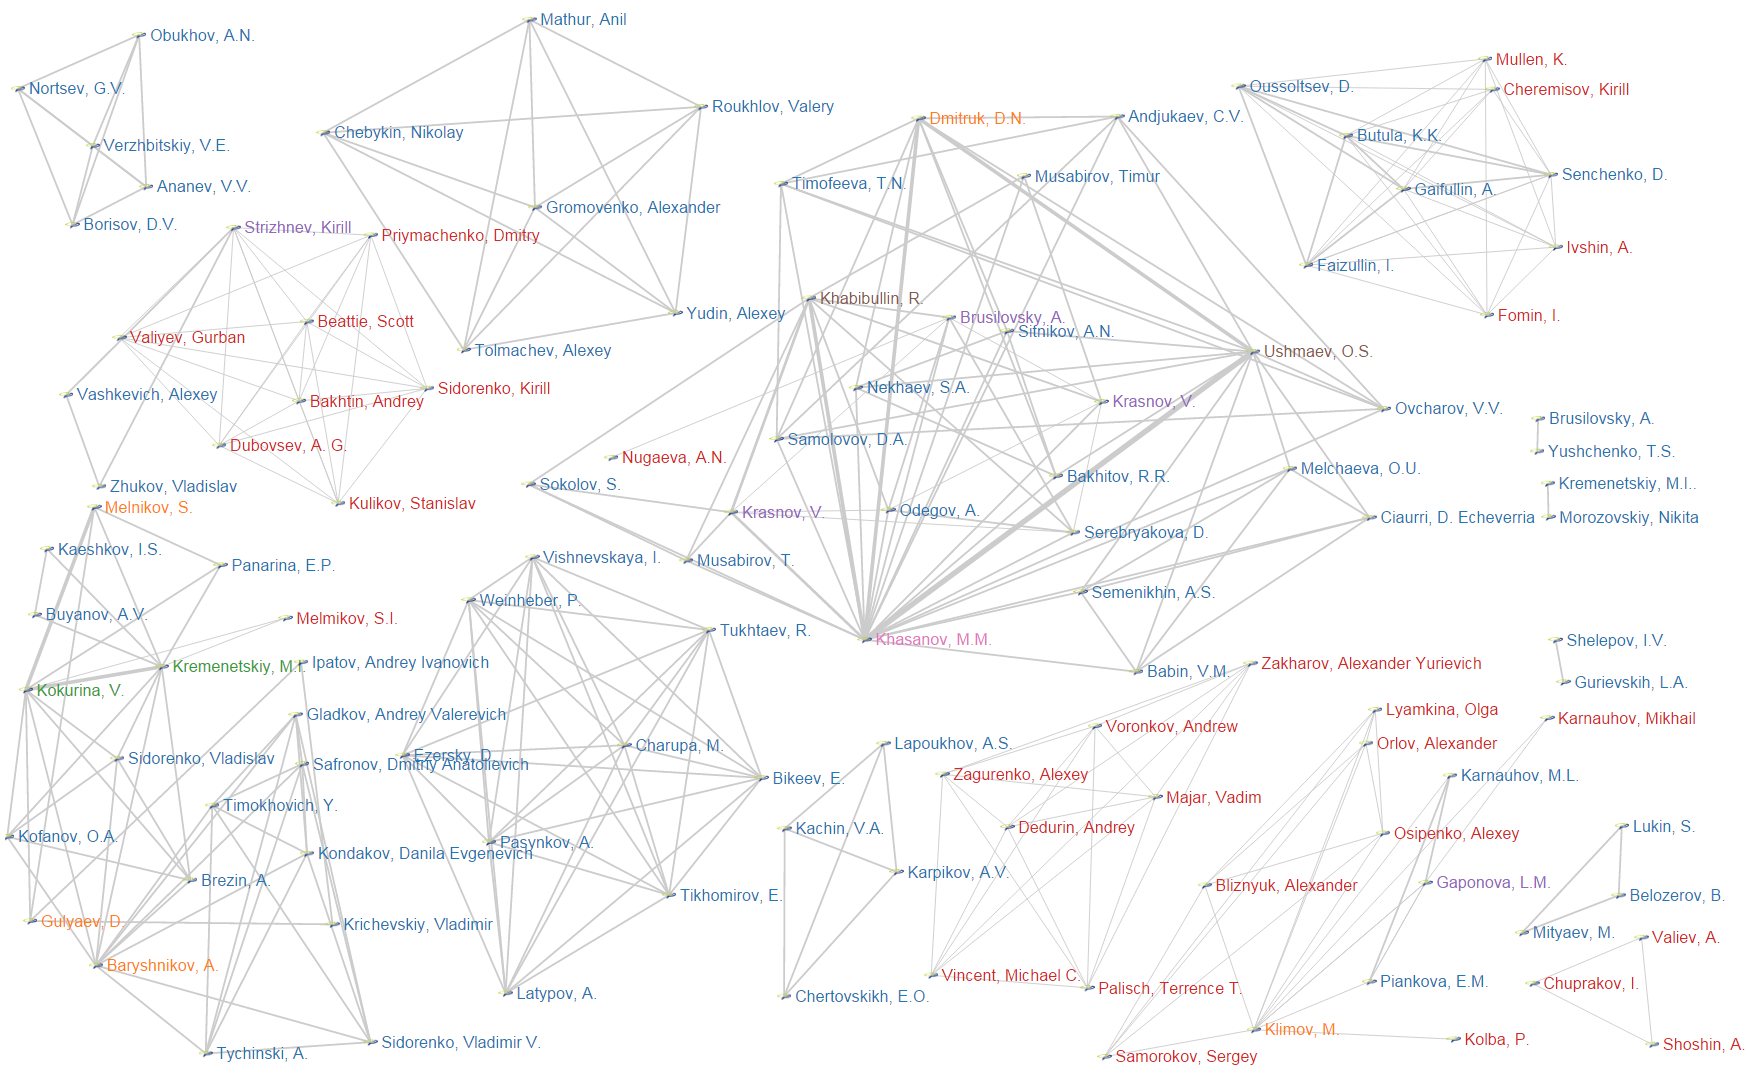
\includegraphics[width=0.8\textwidth]{so3}
  \label{fig:so3}
\end{figure}  

На основании базы публикаций вычислены следующие параметры соавторства:

\begin{enumerate}
\tightlist
\item Среднее количество опубликованных статей на одного автора в год: $ 2 \pm 0.5$
\item Среднее количество соавторов: $2.8 \pm 0.1$
\item Максимальное количество соавторов: $10 \pm 1$
\end{enumerate}

Полученные эмпирические результаты подтверждают результаты имитационного моделирования, что свидетельствует о перспективах применения имитационного моделирования как аналога для моделирования социальных процессов в организационной среде.

\section{Результаты оптимизации процессов научной деятельности}
\label{sec:scrum}
Задача поиска оптимальных параметров команды соавторов для наиболее продуктивного написания научных статей относится к классу задач оптимизации. 
Функция, которую необходимо минимизировать будет зависеть от следующих параметров:

\begin{itemize}
\tightlist
\item
  Количество сотрудников в организационной среде ($N_{o}$);
\item
  Скорость появления новых сотрудников ($Vemp_{new}$);
\item
  Скорость увольнения сотрудников ($Vemp_{fired}$);
\item
  Максимальное количество компетенций у сотрудника ($Cmax_{emp}$);
\item
  Максимальное количество компетенций необходимых для достижения цели исследования ($Cmax_{pub}$).
\end{itemize}

Показателями производительности процесса написания статей, оптимальные значения которых необходимо найти, могут быть следующие:

\begin{itemize}
\tightlist
\item
  Время написания научной статьи ($T_{pub}$)
\item
  Доля сотрудников, опубликовавших статьи от всего количества
  сотрудников ($Frac_{pub}$)
\item
  Доля несостоявшихся статей ($Frac_{notpub}$).
\end{itemize}

Параметрами организационной среды будут следующие:

\begin{itemize}
\tightlist
\item
  Минимальное и максимальное количество сотрудников в организации
  ($N_{omax}$,$N_{omin}$)
\item
  Скорость появления потенциальных целей исследований ($V_{pub}$)
\item
  Временные ограничения на написание статьи ($T_{eoc}$)
\item
  Скорость встреч для заведения знакомств между сотрудниками
  ($V_{friending}$)
\item
  Скорость встреч участников с потенциальными целями
  ($V_{go}$)
\end{itemize}

Исходя из вышеописанных параметров фитнесс-функция $\mathcal{F}$ для оптимизации может быть записана в следующем виде (\ref{eq:scrum5}):

\begin{equation} 
\label{eq:scrum5}
\mathcal{F}\bigg\{ \frac{1}{Frac_{pub}}, T_{pub}, Frac_{notpub} \bigg\} \rightarrow \, min
\end{equation}

При выполнении системы основных условий:

\begin{equation} 
\left\{ \begin{array}{rcl}
N_o \in [ N_{omin}, N_{omax} ]\\ 
Cmax_{emp} \leq Cmax_{pub} \in [ 1, N_{comp} ]\\
Vemp_{new} \geq Vemp_{fired} \geq 0
\end{array}\right.
\label{eq:scrum6}
\end{equation}

Оптимизационный эксперимент был проведен в среде AnyLogic для моделей, с применением Scrum и без. 
Графы соавторств с применением Scrum не изменились.
На основании оптимизационного эксперимента была произведена калибровка имитационной модели соавторства разработанной автором данного исследования. 
Были найдены оптимальные параметры $N_{o}$,$Vemp_{new}$, $Vemp_{fired}$,$Cmax_{emp}$,$Cmax_{pub}$ для Газпромнефть НТЦ. 
Оптимальные значения параметров приведены в Таблице \ref{tab:ex1}.

\begin{table}[H]
\centering
\caption{Оптимальные значения параметров}
\label{tab:ex1}
\resizebox{\textwidth}{!}{%
\begin{tabular}{|l|c|}
\hline
\textbf{Название параметра} & \textbf{Значение параметра} \\ \hline
Количество сотрудников в организационной среде ($N_o$) &  136 \\ \hline
Скорость появления новых сотрудников ($Vemp_{new}$) & 1 сотрудник в неделю \\ \hline
Скорость увольнения сотрудников ($Vemp_{fire}$) & 1 сотрудник в месяц \\ \hline
Максимальное количество компетенций у сотрудника ($Cmax_{emp}$) &  4 \\ \hline
Максимальное количество компетенций необходимых для достижения цели ($Cmax_{pub}$) & 5 \\ \hline
\end{tabular}
}
\end{table}

Калиброванная модель стала основой для исследования эффекта от введения Scrum ролей в процесс написания научных статей.
Для выбранных в разделе показателей производительности $T_{pub}$ и $Frac_{notpub}$ была проведена много прогонная симуляция двух типов: с использованием методики Scrum и без Scrum. 
Анализ данных был произведен в статистической среде $R$.

Результаты попрогонного изменения $T_{pub}$ и $Frac_{notpub}$ приведены на рисунках \ref{ex:fig12} и \ref{ex:fig13} соответственно.
\begin{figure}[H]
  \caption{ Среднее время публикации статей в зависимости от номера прогона. Линиями нарисована зависимость скользящего среднего.}
  \centering
    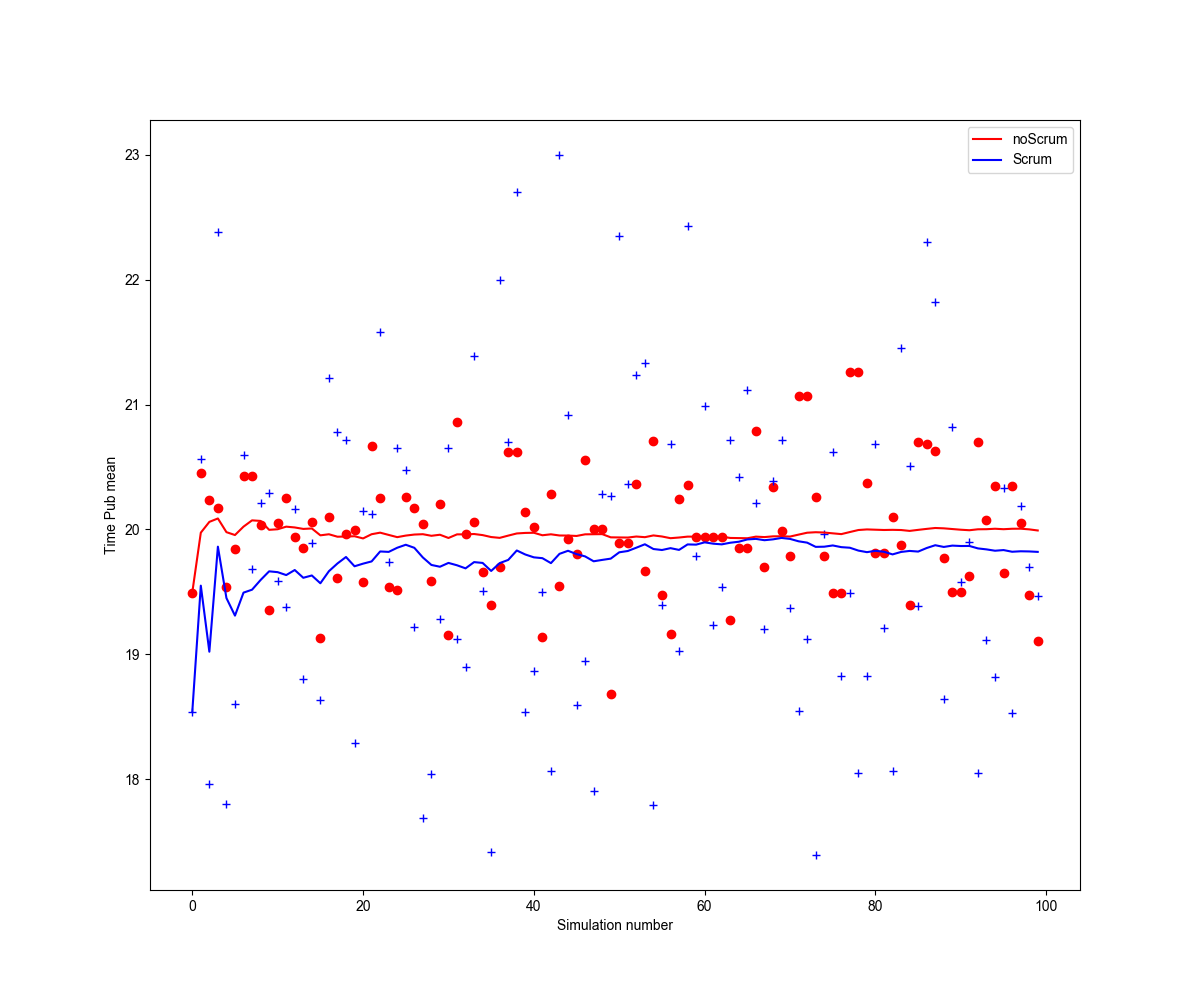
\includegraphics[width=0.8\textwidth]{scrum-img12}
  \label{ex:fig12}
\end{figure}  

\begin{figure}[H]
  \caption{Доля несостоявшихся научных статей в зависимости от номера прогона. Линиями нарисована зависимость скользящего среднего.}
  \centering
    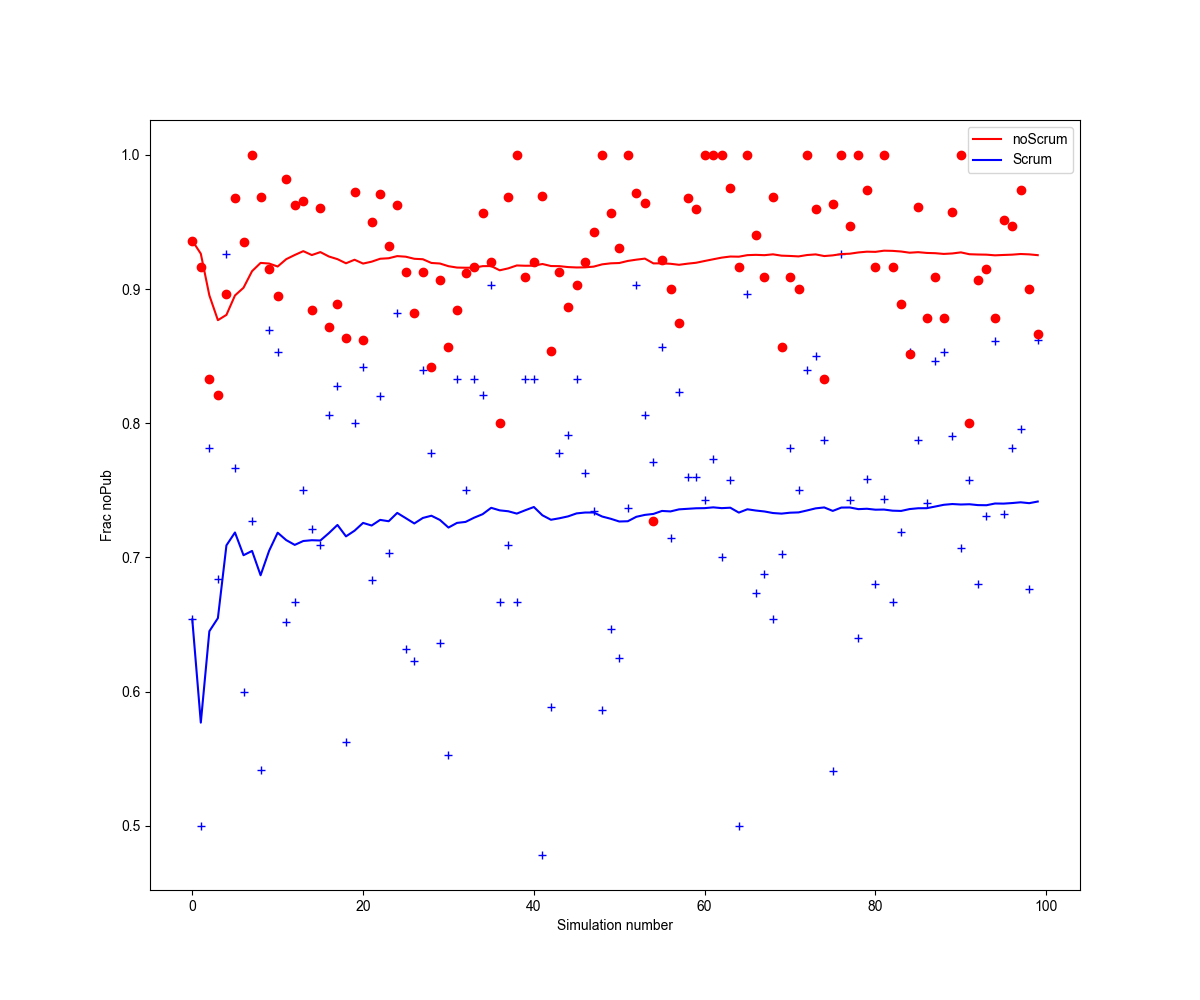
\includegraphics[width=0.8\textwidth]{scrum-img13}
  \label{ex:fig13}
\end{figure}  

Для оценки влияния Scrum на время написания статей $T_{pub}$, автор сравнил время написания статей для двух выборок методом t-теста для сравнения двух независимых выборок.
Результаты показали, что на уровне 1\% значимости длительность написания статей с использованием Scrum не изменяется.

\begin{itemize}
\tightlist
\item
  Среднее время написания научной статьи со Scrum составило 19.90 недель со стандартным отклонением 3.33 недели.
\item
  Среднее время написания научной статьи без Scrum составило 19.90 недель со стандартным отклонением 0.77 недели
\end{itemize}

Автор также дополнительно использовал непараметрический критерий U Манна-Уитни в случае, при котором распределении признаков не соответствует нормальному распределению, результаты которого оказались аналогичны t-тесту.
Полученные результаты свидетельствуют о том, что использование Scrum не ускоряет написание статей, даже при условии того, что функция написания статей не подчиняется нормальному распределению.

Другим показателем, который может быть использован для оценки продуктивности Scrum, является доля \emph{несостоявшихся научных статей}. 
Мы оценили долю \emph{несостоявшихся научных статей} для команд, использующих Scrum и не использующих.

\begin{itemize}
\tightlist
\item
  Доля \emph{несостоявшихся научных статей} в командах, использующих
  Scrum 0.74 со стандартным отклонением 0.02
\item
  Доля \emph{несостоявшихся научных статей} в командах, не использующих
  Scrum составляет 0.92 со стандартным отклонением 0.01
\end{itemize}

Другими словами, из 100\% начатых статей в командах, использующих Scrum, успешными будут 26\% статей. 
В случае, если Scrum не используется, во временные рамки публикационного процесса с требуемым качеством уложатся 8\% статей.

\section{Прогнозирование соавторства}

Коллективное соавторство в написании научных статей имеет детерминированную и случайную структурные составляющие. 
Кроме рациональных аспектов при образовании коллектива соавторов отдельной научной статьи существуют и эмоциональные составляющие. 
Во временной перспективе складываются и распадаются рабочие группы исследователей, обновляется трудовой коллектив и состав подрядчиков, которые участвуют в совместных отраслевых коллаборациях для проведения исследований.

Несмотря на всю сложность соавторства, существуют несколько классов моделей для симуляции образования соавторства. 
В их числе модели на основании случайных графов и модели образования соавторств на основе компетенций соавторов. 
Оба математических аппарата разработаны и применяются в течении нескольких десятков лет по отдельности. 
Но практических применений моделей соавторств в корпоративной практике не так много.

Автор выдвинул гипотезу о том, что необходимо объединить несколько различных типов моделей для того, чтобы лучше понять природу научных коллабораций в отдельной организации. 

Автор данного исследования поставил задачу разработать методику построения модели соавторства для научно-технического центра, учитывающую различные структурные составляющие соавторства. 

В результате автор разработал модель с использованием методов машинного обучения, случайных графов и модели компетенций. 
На основании разработанной модели сделан прогноз развития соавторства в написании научных статей научно-технического центра Газпромнефть.

Практическая ценность результатов данного исследования состоит в следующем: Количественно оценен вклад различных структурных составляющих в формировании соавторств при написании научных статей.

Прогнозирование развития соавторства в написании научных статей позволяет осуществить 
планирование корпоративных ресурсов для поддержания роста научных публикаций.
Понимание кластерной структуры соавторства позволяет производить выравнивание направлений научной деятельности в соответствии со стратегическим планом развития научно-технического центра.


Измерение деятельности научно-исследовательских организаций на основании графа соавторства является хорошо зарекомендовавшей себя практикой. 
Исследователи показывают возможности выявления наиболее производительных авторов (``Highly Productive Authors'') и влиятельных авторов (``Influential Authors''). 

В качестве объекта исследования была выбрана публикационная активность НТЦ Газпромнефть. 
Данные были получены из открытой электронной библиотеки OnePetro международного сообщества нефтегазовых инженеров (SPE). 
После очистки было получено 172 статьи. 
Распределение авторов по годам отображено на рисунке (Рис. \ref{fig:guest2}).

\begin{figure}[H]
  \caption{Распределение авторов по годам.}
  \centering
    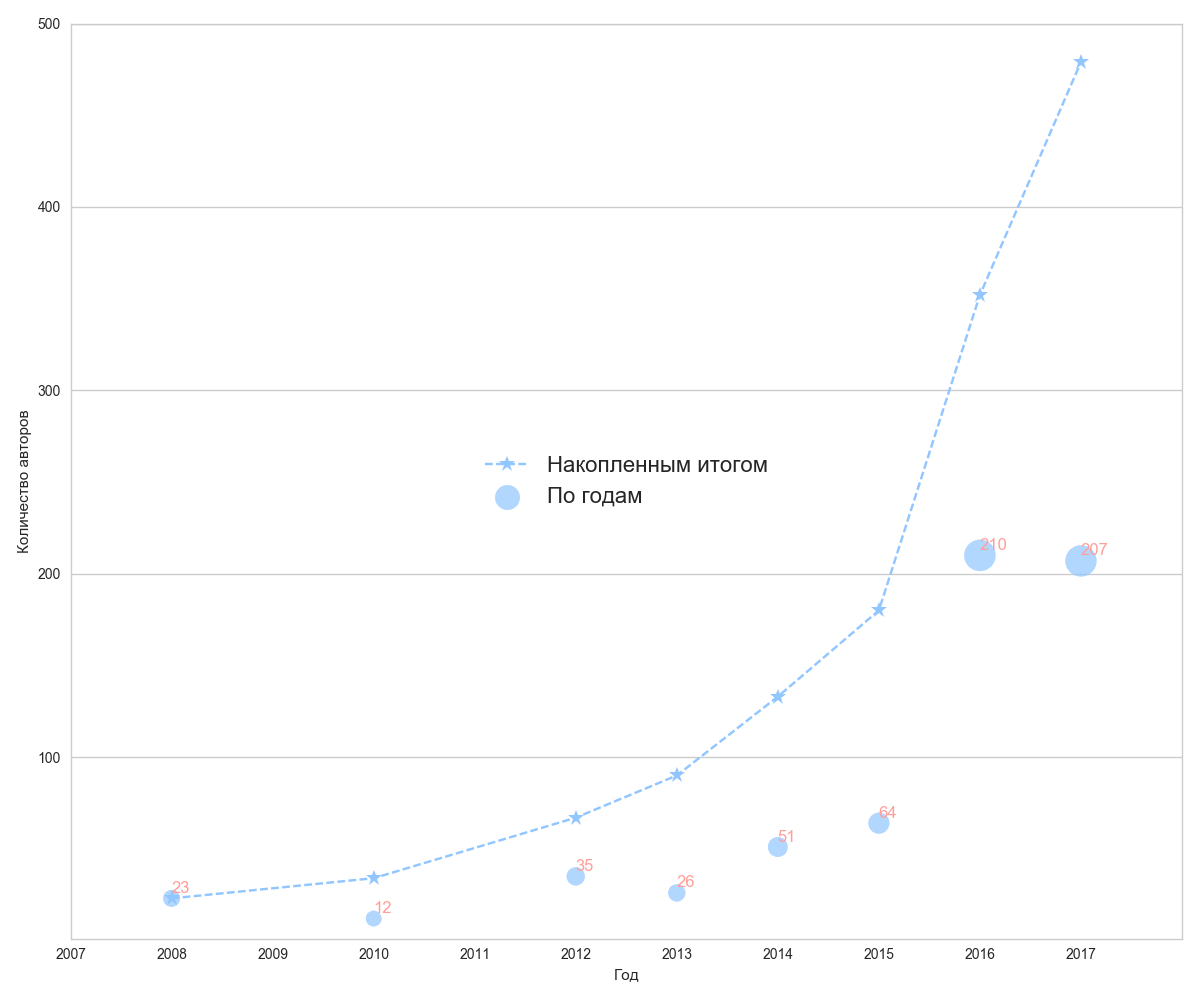
\includegraphics[width=0.8\textwidth]{guest2}
  \label{fig:guest2}
\end{figure}  

Прямолинейным ответом на поставленный исследовательский вопрос может быть интерполяция кривой роста количества авторов.
В результате такой оценки получим  следующую зависимость  $y=13.3816e^0.3422x$ с достоверностью $R^2=0.98$, дающей прогноз 585 авторов в 2018 году. 
Но из графика  \ref{fig:guest2} мы так же видим, что количество авторов в 2017 году (207) меньше чем в 2016 году (210), что может оказаться насыщением роста и повлиять на прогноз.

Построим прогноз на основании графа соавторства. 
Для этого построим двудольный граф соавторства с вершинами: автор (479) и статья (171). 
Авторы обладают техническими компетенциями, статьи характеризуются названием, годом издания и ключевыми словами.

Полученный граф соавторства имеет 26 связанных компонент наибольшая из которых содержит 556 вершин, а остальные – не более 8. 
Малые связанные компоненты относятся к авторам, написавшим свою первую статью. Наличие малых связанных компонент можно рассматривать, как одну из составляющих роста графа соавторств. 
В таблице (Таб. \ref{tab:guest1}) приведены количества и размеры связанных компонент за каждый год нарастающим итогом. 

\begin{table}[H]
\centering
\caption{Размеры связанных компонент графа соавторств по годам нарастающим итогом.}
\label{tab:guest1}
\resizebox{\textwidth}{!}{%
\begin{tabular}{|l|l|l|}
\hline
\textbf{Год} & \textbf{Размеры связанных компонент} & \textbf{Доля малых компонент} \\ \hline
2017 & 556, 8, 8, 8, 6, 5, 5, 5, 4, 4, 4, 4, 4, 4, 3, 3, 3, 2, 2, 2, 2, 2, 2, 2, 2, 2 & 15\% \\ \hline
2016 & 367, 8, 8, 8, 8, 8, 6, 5, 5, 5, 5, 4, 4, 4, 4, 3, 3, 3, 2, 2, 2, 2, 2, 2, 2, 2 & 23\% \\ \hline
2015 & 89, 22, 21, 15, 12, 12, 8, 8, 8, 8, 6, 6, 5, 4, 3, 3, 2, 2, 2, 2, 2 & 63\% \\ \hline
2014 & 46, 18, 15, 12, 12, 10, 8, 8, 8, 7, 6, 5, 4, 4, 3, 2, 2, 2, 2, 2 & 74\% \\ \hline
2013 & 23, 15, 12, 11, 10, 8, 8, 7, 5, 4, 4, 4, 2, 2, 2 & 80\% \\ \hline
2012 & 15, 14, 12, 11, 8, 8, 7, 4, 4, 4 & 83\% \\ \hline
2010 & 12, 9, 8, 8, 4, 3 & 73\% \\ \hline
2008 & 12, 8, 7, 3 & 60\% \\ \hline
\end{tabular}%
}
\end{table}

Таким образом мы видим, что граф соавторства прогрессирует в сегменте малых связанных компонент по количеству и вместе с тем граф становится более связанным – увеличивается количество узлов в главной связанной компоненте. Для уточнения прогнозирования целесообразно будет учесть такое строение. 
На Рис. \ref{fig:guest3} приведена инкрементальная динамика прироста графа соавторства по годам. Уточним, что граф соавторств 2017 года является суммой всех изображенных на (Рис. \ref{fig:guest3}).

\begin{figure}[H]
  \caption{Динамика прироста развития графа соавторств по годам.}
  \centering
    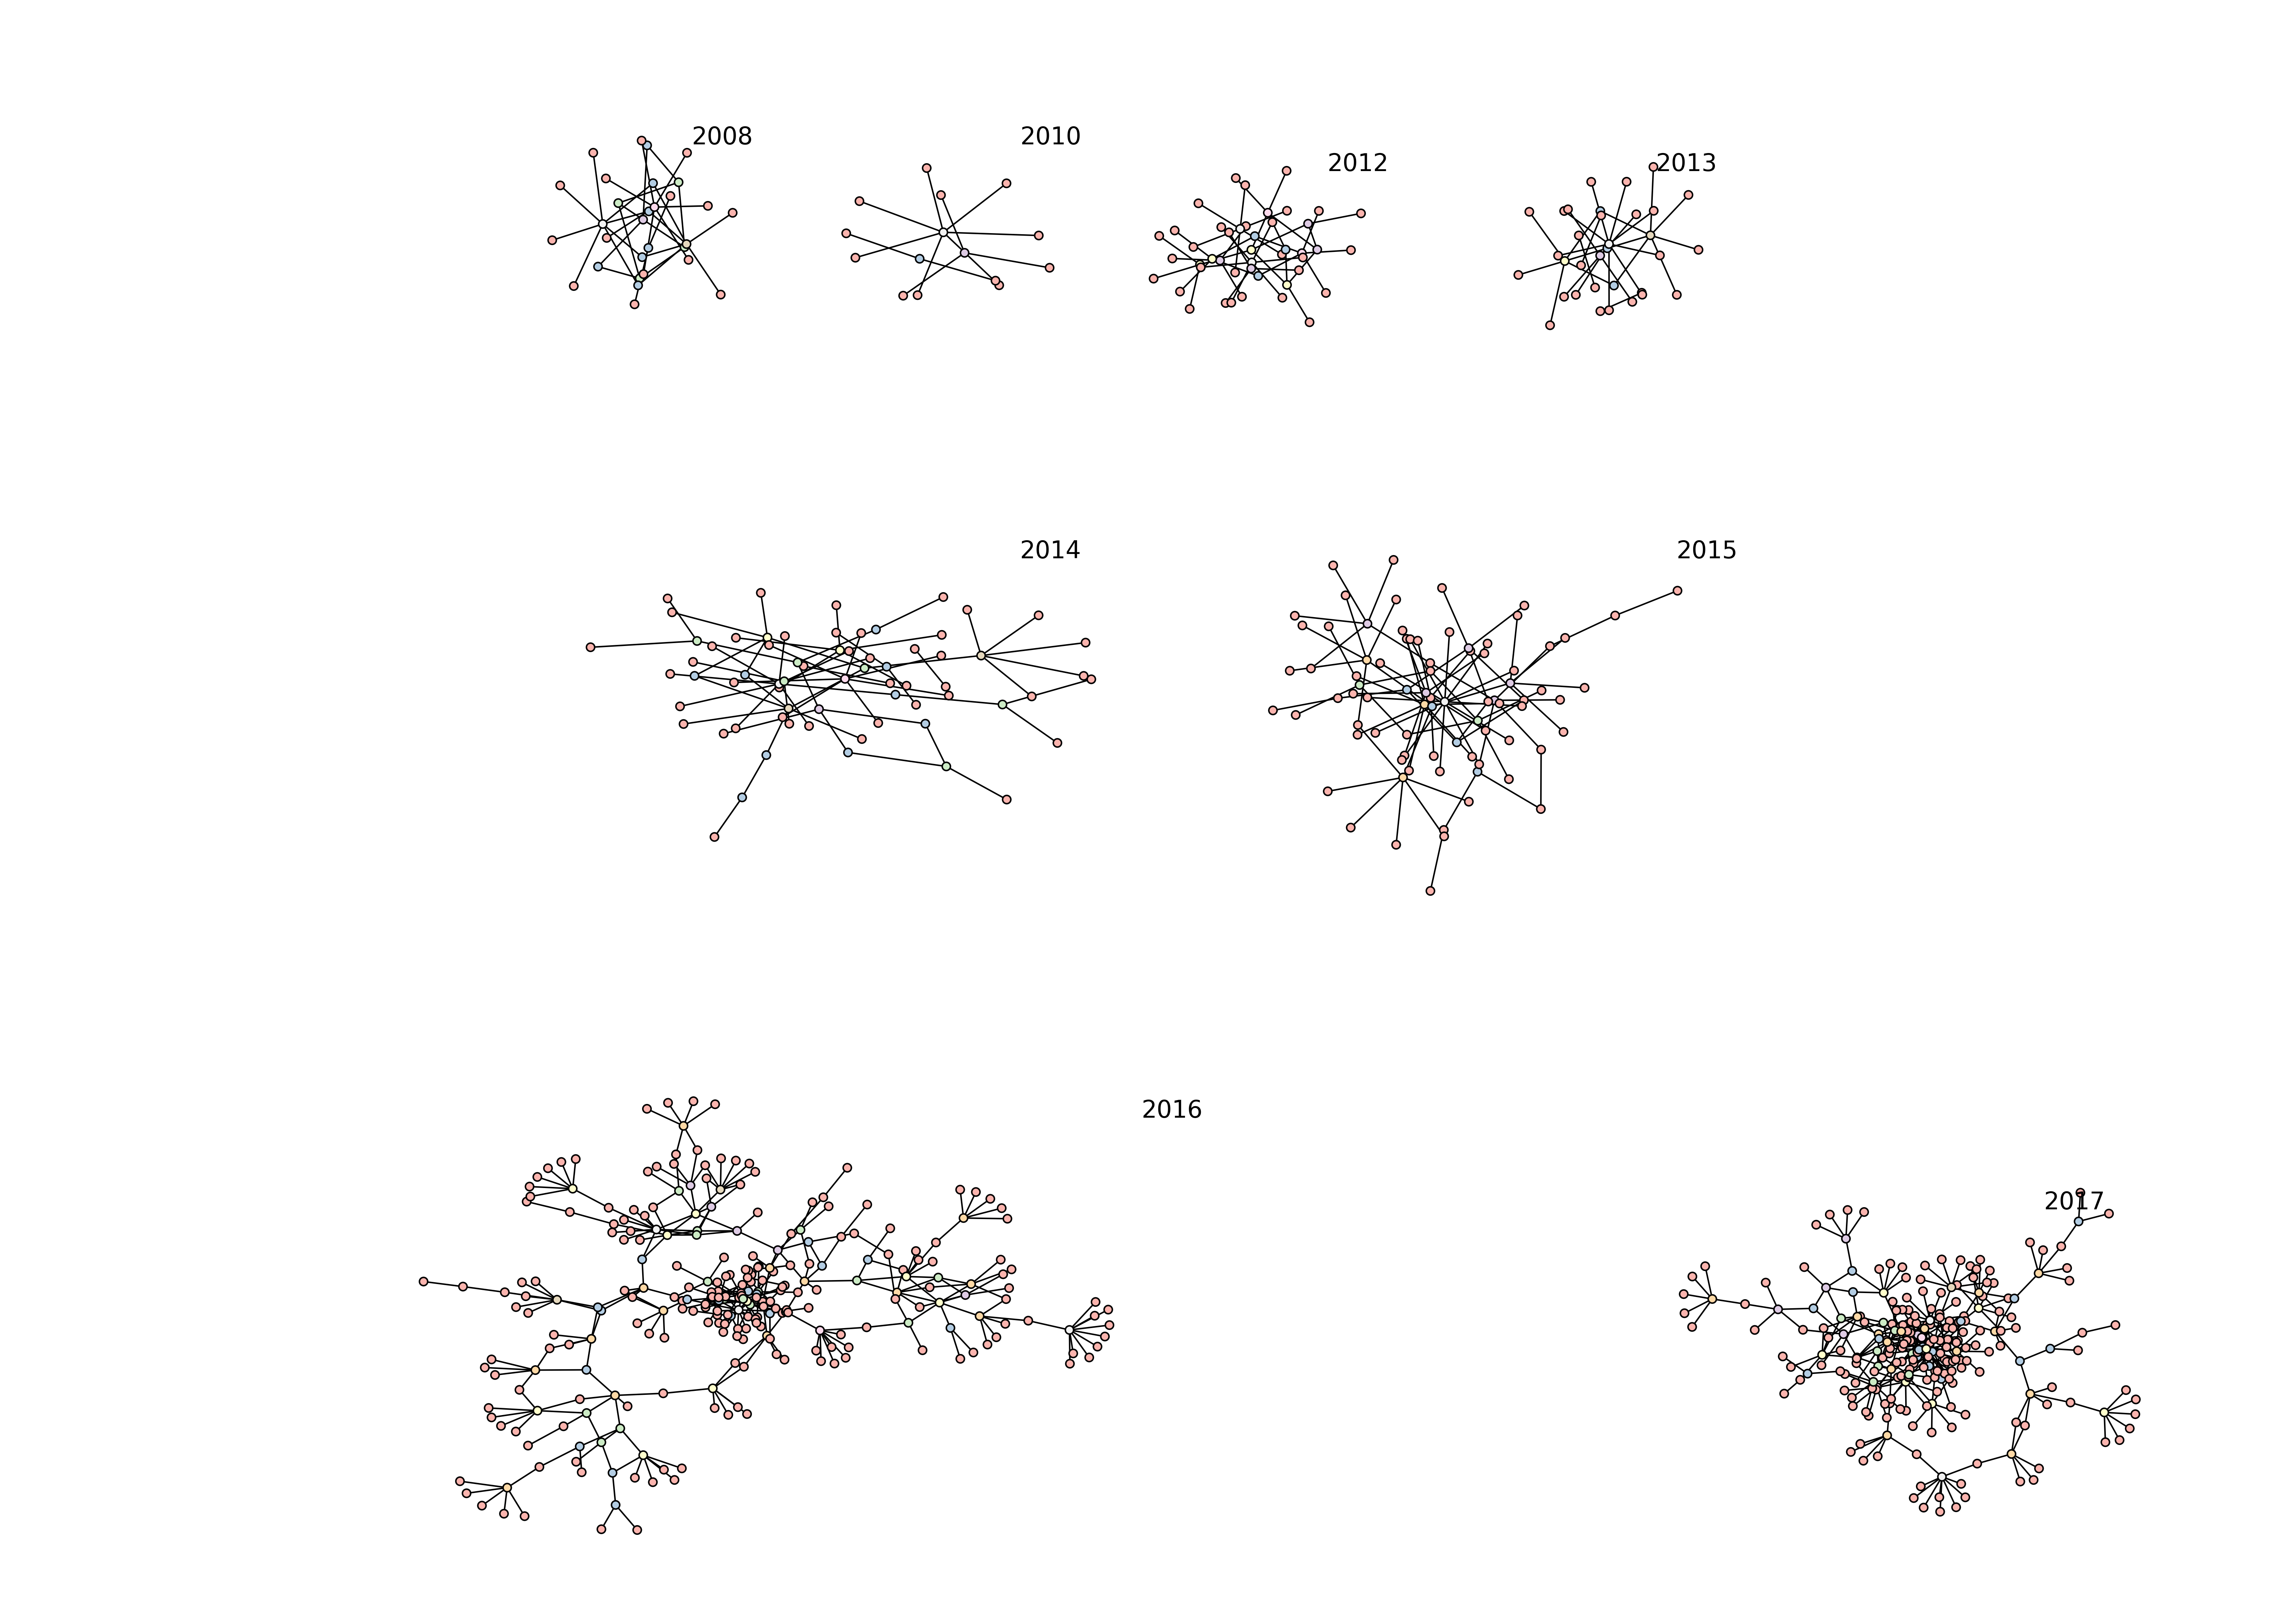
\includegraphics[width=0.99\textwidth]{guest3}
  \label{fig:guest3}
\end{figure}  

Из рисунка (Рис. \ref{fig:guest3}) можно сделать качественной вывод об увеличении ежегодно прибавляемых к графу соавторства связей. Изменение роста ведет к усложнению структуры графа соавторства в 2016 году, что можно констатировать как ``эффект локтя''.Для прогнозирования авторства будем использовать следующие метрики вершин графа:
\begin{itemize}
\tightlist
\item Degree centrality
\item Betweenness centrality
\item Closeness centrality
\item Harmonic centrality
\item Clustering
\end{itemize}

Распределения метрик вершин графа соавторства приведены на рисунке (Рис.\ref{fig:guest4}).

\begin{figure}[H]
  \caption{Метрики вершин графа соавторства.}
  \centering
    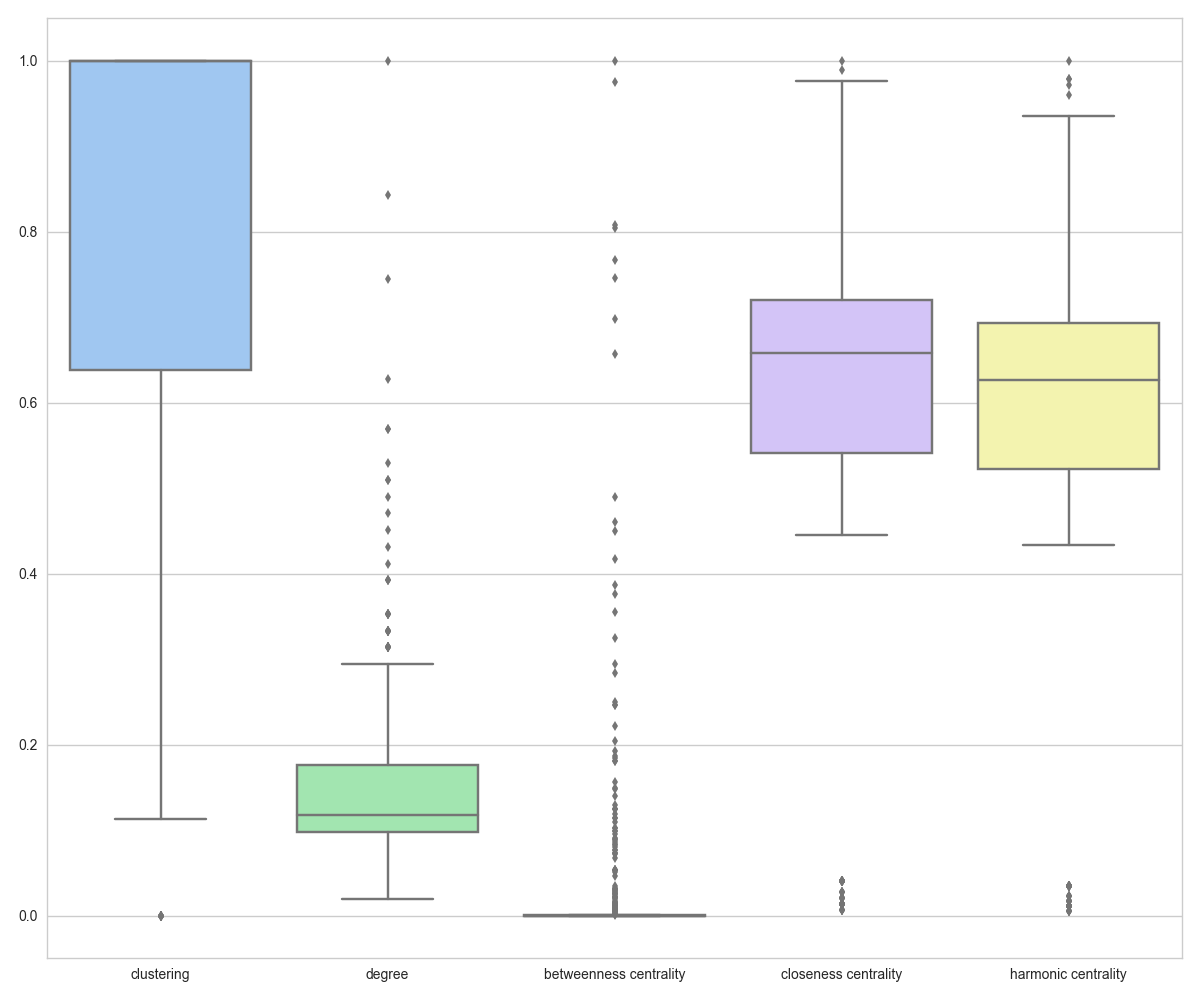
\includegraphics[width=0.8\textwidth]{guest4}
  \label{fig:guest4}
\end{figure}  

Для прогнозирования авторства будем использовать модель бинарной классификации. Выбор модели будем производить на основе ROC-кривой. Обучения модели будем производить на метриках 2016 года. Параметры моделей оптимизированы с помощью кросс-валидации с 5-кратным фолдингом. В результате сравнения различных классификаторов были получены следующие результаты (Таб. \ref{tab:guest2} ).

\begin{table}[H]
\centering
\caption{Сравнение классификаторов по метрике ROC AUC.}
\label{tab:guest2}
\resizebox{\textwidth}{!}{%
\begin{tabular}{|l|l|}
\hline
\textbf{Модель} & \textbf{ROC AUC} \\ \hline
KNeighborsClassifier & 0.66 \\ \hline
RidgeClassifier & 0.73 \\ \hline
RandomForestClassifier & 0.72 \\ \hline
SVM & 0.70 \\ \hline
Multi-layer perceptron & 0.75 \\ \hline
\end{tabular}%
}
\end{table}

Лучшее значение метрики ROC AUC показал классификатор на основе нейронной сети (Multi-layer perceptron) с одним слоем из 10 персептронов. 
Отчет о выполнении прогноза авторства в 2018 году на основе графа соавторства 2017 года приведен в таблице (Таб. \ref{tab:guest3}).

\begin{table}[H]
\centering
\caption{Отчет о выполнении прогноза авторства на 2018 г.}
\label{tab:guest3}
\resizebox{\textwidth}{!}{%
\begin{tabular}{|l|l|l|l|l|}
\hline
 & \textbf{precision} & \textbf{recall} & \textbf{f1-score} & \textbf{support} \\ \hline
\textbf{not author} & 0.80 & 0.98 & 0.88 & 66 \\ \hline
\textbf{author} & 0.80 & 0.20 & 0.32 & 20 \\ \hline
\textbf{Avg / Total} & 0.80 & 0.80 & 0.75 & 86 \\ \hline
\end{tabular}%
}
\end{table}

В результате прогнозирования определено 406 авторов в 2018 году. Если добавить к этому прогнозу сотрудников, которые напишут свою первую статью в 2018 году, то на основании оценки по динамике роста связанных компонент получим прибавку в 15\%. Итого в 2018 году авторами станут 467 сотрудников.

\subsection{Распределение научных направлений на основе соавторств}
\label{sec:allo}
Планирование научно-технического развития исследовательской организации должно быть увязано с реальным положением дел. Такие факторы, как организационная инертность, диверсификация исследований и увлечение созданием ИТ-продуктов, могут существенно исказить любые стратегии и планы развития. Тем не менее, исполнимость планов является важной характеристикой развития, существенно повышающей мотивацию персонала к достижению результата. Поэтому постановка реально, а не только ``на бумаге'' выполнимых задач, необходима. 

Не может быть достаточно только количественных инструментов оценки выполнения научно-исследовательских работ. Формально-бумажная отчетность по НИР не способна отразить увлеченность и вовлеченность исследователей в работу. В то время как малые формы исследовательских работ, такие как презентация на научно-технической конференции или научная статья в рецензируемом периодическом издании, требуют намного более неформального отношения со стороны исследователей.  Анализ развития научно-технической организации на основе публикационной активности является распространенной практикой. Многие исследования анализируют корпусы текстов научных статей и делают заключения о трендах развития. Текстовые данные обладают высоким уровнем шума и даже современные методы анализа на основании word embedding выдают точные прогнозы только на основании огромных объемов текстов, которые не всегда имеются у небольших организаций. При этом именно небольшие научно-исследовательские организации в наибольшей степени страдают от неточности планирования научной деятельности.

Современный фокус применения научных подходов к управленческим решениям приобретает все большую актуальность. С увеличением объемов данных традиционные аналитические средства руководителей организаций становятся все менее эффективными. С другой стороны, необходимого объема данных для устойчивой работы современных алгоритмов часто бывает недостаточно. В авангарде этой тенденции возникает задача адаптации и создания новых эвристик для таких классических задач, как кластеризация для применения в организационной среде.

Кластеризация данных на основании статической модели получила развитие с открытием таких алгоритмов, как PAM, CLARANS, DBSCAN, CURE и ROCK. Тем не менее, в последнее время особое внимание привлечено к алгоритмам кластеризации на основании динамической модели, например, CHAMELEON. Основная идея алгоритма CHAMELEON заключается в использовании метрик близости графа, построенного на основании набора кластеризуемых данных с помощью метода ``k наиболее близких соседей'' (KNN). Метрики графа оказываются более эффективными для разбиения данных ``сверху вниз'' в случае сложных объектов.

Разнообразие алгоритмов кластеризации не умаляет важность задачи оценки их качества. Но в условиях ограниченного количества данных и для обеспечения управленческих решений качество кластеризации должно иметь не только математически обоснованную, но и уверенную наглядную составляющую. Другими словами, чтобы ``с одного взгляда было понятно'' и не нужно было вникать в формулы. Таковы требования современного бизнеса.

С формальной точки зрения необходимо решить задачу обучения без учителя (unsupervised machine learning) для графа соавторств, отнести кластеры к определенным тематикам и выявить изменения в кластерах со временем.
Кластеризация графа соавторства может быть осуществлена на основании различных метрик вершин: 
\begin{itemize}
\tightlist
\item Degree centrality
\item Betweenness centrality
\item Closeness centrality
\item Harmonic centrality
\item Clustering
\end{itemize}

Рассмотрим содержательный смысл метрики Betweenness centrality применительно к задаче кластеризации графа соавторств научно-технической организации. Метрика Betweenness centrality характеризует то, насколько данный узел важен для связанности графа. Связи в графе соавторств отражают совместную исследовательскую работу. Графы соавторств не всегда являются связанными, обычно это несколько связанных компонент разного размера. 

Связанные компоненты являются естественными кластерами. Небольшие связанные компоненты отражают начальные инициативы – это первые статьи сотрудников. Но главная связанная компонента может содержать 90\% вершин графа соавторства и нуждается в отдельном подходе к кластеризации. 

Для выделения кластеров из главной связанной компоненты графа соавторств возможно использовать методику искусственного удаления вершин с наибольшей метрикой Betweenness centrality. При каждом таком удалении вершины граф может распадаться на несколько несвязанных компонент. На рисунке (Рис.\ref{fig:allo2}) приведена модель такого разделения.

\begin{figure}[H]
  \caption{Модель разделения графа. а.Связанный изначальный граф. б.Тот же граф, но после удаления вершины с наибольшей метрикой Betweenness centrality уже представляет две связанных компоненты.}
  \centering
    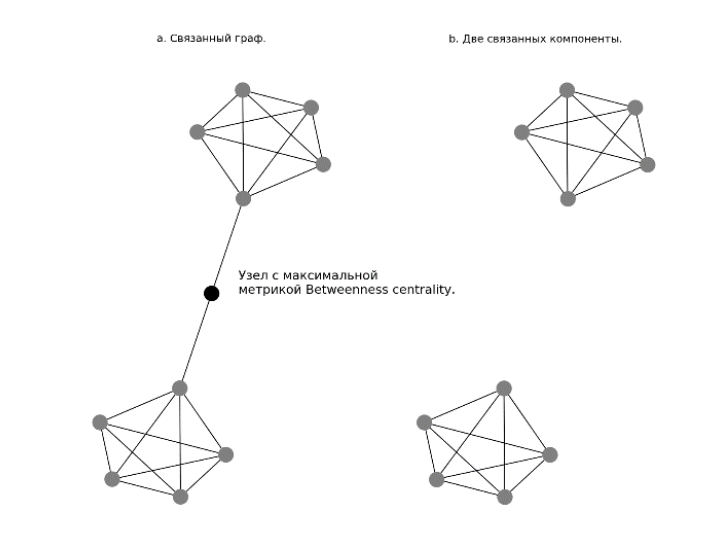
\includegraphics[width=0.8\textwidth]{allo2}
  \label{fig:allo2}
\end{figure}  

Каждую из получившихся при таком распаде связанных компонент можно анализировать на однородность тематики на основании текстов статей, которыми она образована. В результате нескольких итераций мы получим набор кластеров.
Предложенный автором метод является эвристическим и нуждается в проверке по определенному формальному критерию. Для задач кластеризации таким критерием принято считать метрики близости объектов в кластере и расстояния между объектами в разных кластерах.

Сходимость данного метода обеспечивается путем поиска минимума функционала ошибок определения кластеров:

\begin{equation}
\vert WSS - BSS \vert \rightarrow min , 
\label{eq:allo1}
\end{equation}
где $WSS$ - это функция связанности кластера $C_i$:

\begin{equation}
WSS = \sum_i \sum_{x \in C_i} ( x - m_i)^2 , 
\label{eq:allo2}
\end{equation}
а $BSS$ это функция разделения кластеров $C_i$:

\begin{equation}
BSS = \sum_i \vert C_i \vert ( m - m_i)^2 , 
\label{eq:allo3}
\end{equation}
где $\vert C_i \vert $ - это размер кластера $C_i$.

Междисциплинарные исследования приводят к тому, что статьи будут относится к нескольким тематикам, так что полученные кластера будут пересекающимися – не эксклюзивными. Таккая кластеризания называется"мягкой".

В качестве объекта исследования была выбрана публикационная активность НТЦ ``Газпромнефть''. Данные были получены из открытой электронной библиотеки OnePetro международного сообщества нефтегазовых инженеров (SPE). После очистки было получено 172 статьи.
Построим прогноз на основании графа соавторства. Для этого построим двудольный граф соавторства с вершинами: автор (479) и статья (171). Авторы обладают техническими компетенциями, статьи характеризуются названием, годом издания и ключевыми словами.
Полученный граф соавторства имеет 26 связанных компонент наибольшая из которых содержит 556 вершин, а остальные не более 8. Связанные компоненты с количеством узлов до 8 являются считать первыми статьями сотрудников.
Рассмотрим наибольшую связанную компоненту (556 вершин). Выделим подграф из основного графа соавторства на основании узлов, относящихся к наибольшей связанной компоненте. Получившийся подграф отображен на рисунке (Рис. \ref{fig:allo3}).

\begin{figure}[H]
  \caption{Подграф наибольшей связанной компоненты графа соавторства.}
  \centering
    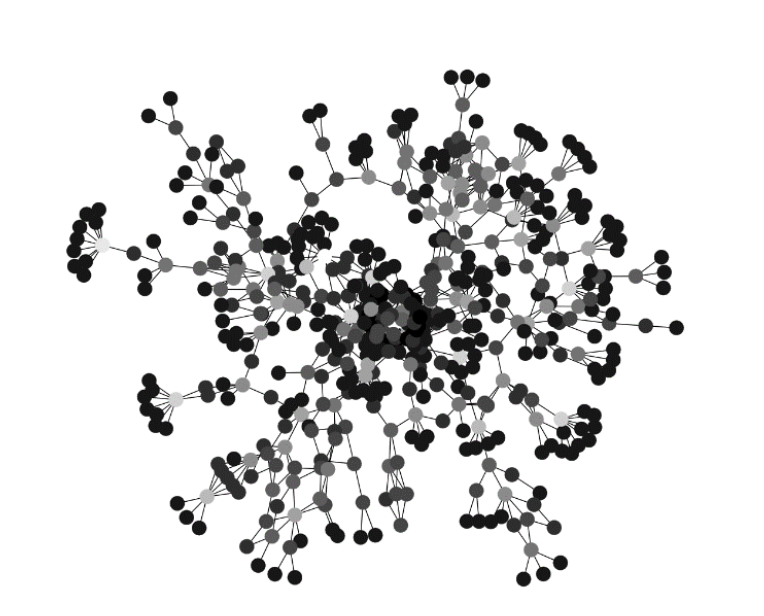
\includegraphics[width=0.8\textwidth]{allo3}
  \label{fig:allo3}
\end{figure}  

Рассчитаем для полученного подграфа метрику Betweenness centrality. Полученные значения Betweenness centrality отображены на рисунке (Рис. \ref{fig:allo4}). Нулевые значения Betweenness centrality не отображены.

\begin{figure}[H]
  \caption{Гистограмма значений Betweenness centrality для подграфа наибольшей связанной компоненты графа соавторств.}
  \centering
    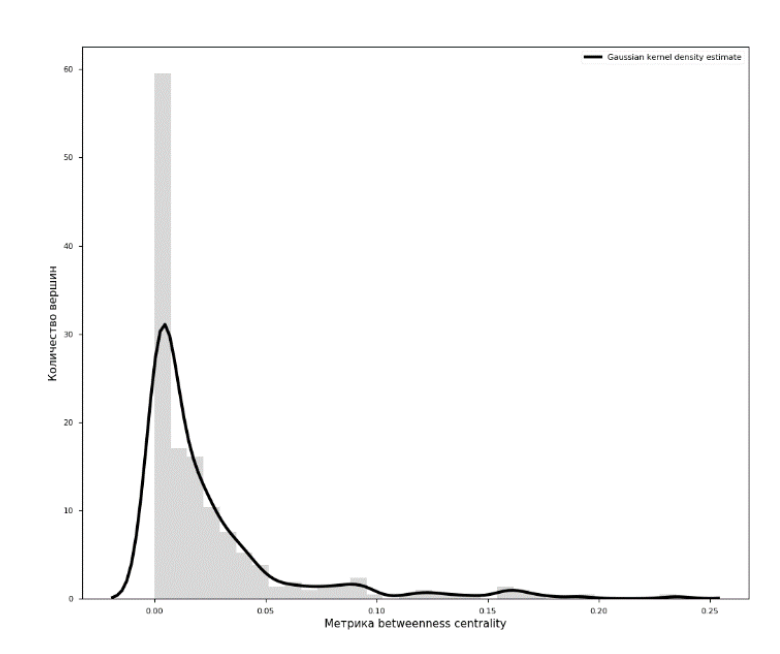
\includegraphics[width=0.8\textwidth]{allo4}
  \label{fig:allo4}
\end{figure}  

Как мы видим из Рис. \ref{fig:allo4} значения метрики Betweenness centrality в третьем квартиле принадлежат всего 23 вершинам, что составляет менее 5 \% от всего количества вершин.
Применим алгоритм искусственного удаления вершин с наибольшим значением метрики Betweenness centrality. На рисунке (Рис. \ref{fig:allo5}) отображена зависимость количества связанных компонент от количества искусственно удаленных вершин

\begin{figure}[H]
  \caption{Зависимость количества связанных компонент от количества искусственно удаленных вершин.}
  \centering
    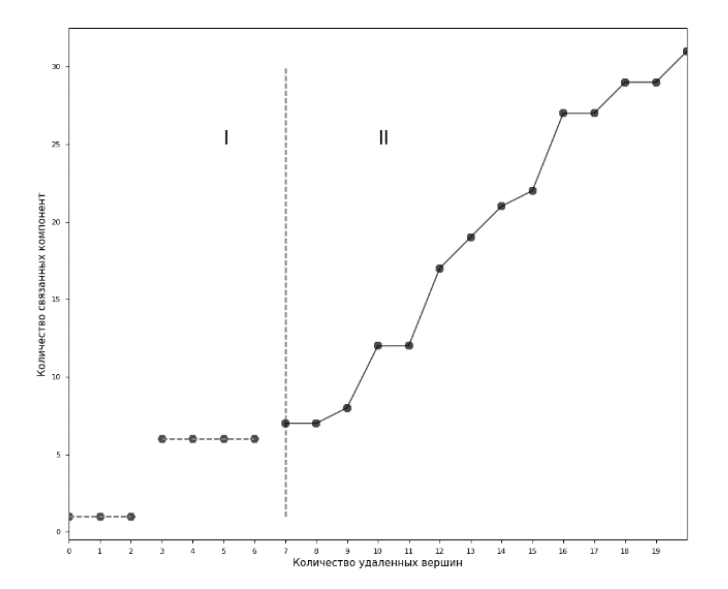
\includegraphics[width=0.8\textwidth]{allo5}
  \label{fig:allo5}
\end{figure}  

При удалении вершин поведение графа происходит в двух режимах:

\begin{enumerate}[I/]
\item Удержание связанности
\item Экспоненциальный распад
\end{enumerate}

Отличительной чертой режима I является то, что граф остается связанным при удалении вершин с высокими значениями метрики Betweenness centrality. Это означает, что удаляемые вершины не являются единственными связующими между кластерами.
Отличительной особенностью режима II является следование степенной модели распада графа, когда удаление каждого узла вызывает степенной рост появления новых связанных компонент.
Рассмотрим более подробно вторую половину режима I алгоритма, когда граф разделился на 6 связанных компонент. Размеры этих компонент составляют 511, 34, 1, 1, 1, 1. И среди них ярко выраженное направление исследований по Теме 1 представлено именно компонентой с 34 узлами, представленной на рисунке (Рис. \ref{fig:allo6}).

\begin{figure}[H]
  \caption{Кластер исследователей по Теме 1, выделенный в результате применения метода удаления вершин в наибольшим значением метрики Betweenness centrality.}
  \centering
    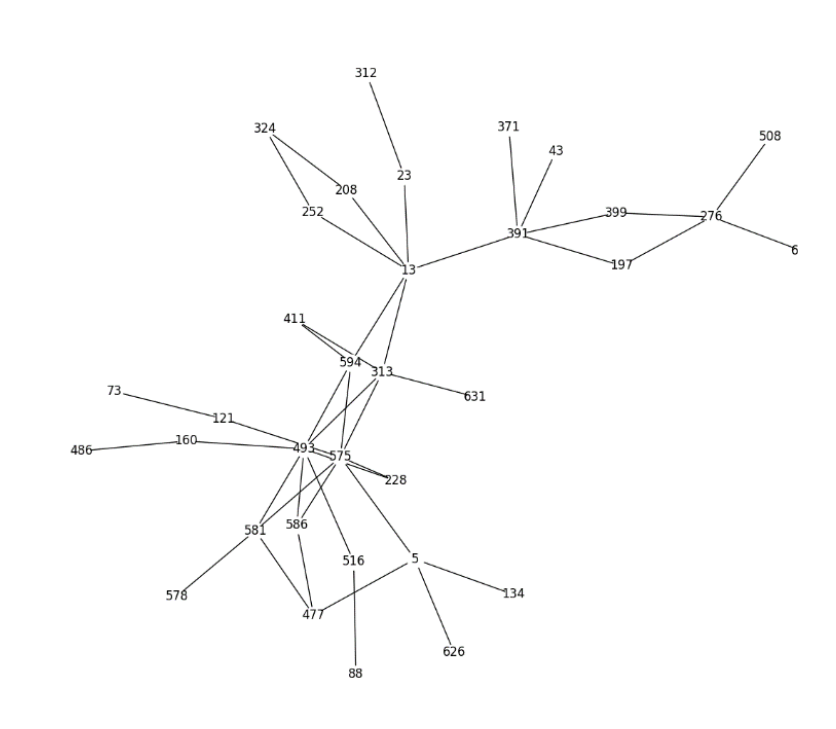
\includegraphics[width=0.8\textwidth]{allo6}
  \label{fig:allo6}
\end{figure}  

Мы рассмотрели выделение одного кластера подробно. Полный алгоритм выделения кластеров будет состоять из следующих шагов:
\begin{enumerate}
\tightlist
\item Построение двудольного графа соавторств: $G$
\item Определение метрики Betweenness centrality для графа $G$
\item Определение вершины с максимальной метрикой $N_{max(Betweenness centrality)}$
\item Удаление вершины $N_{max(Betweenness centrality)}$ из графа $G$
\item Получение списка связанных компонент графа $G$
\item Вычисление метрики качества полученных кластеров $BSS$ и $WSS$
\item Далее алгоритм повторяется для каждой связанной компоненты
\item Алгоритм завершается, когда все связанные компоненты представляют кластеры удовлетворительного качества.
\end{enumerate}

Для выбранного графа соавторства были выделены 16 кластеров.
Для вычисления значений  и W на основании текстов статей было использовано векторное представление текста статьи (VSM). Каждая статья представлена в виде вектора со значениями метрики BM25 для каждого слова. Статьи рассматривались как ``мешок слов'' (bag of words). Для измерения дистанции между векторными представлениями статей была использована косинусная мера.
На рисунке (Рис. \ref{fig:allo7}) изображена матрица раздельности кластеров .

\begin{figure}[H]
  \caption{Матрица раздельности кластеров. По осям отображены номера кластеров. В ячейках значения функции $BSS$.}
  \centering
    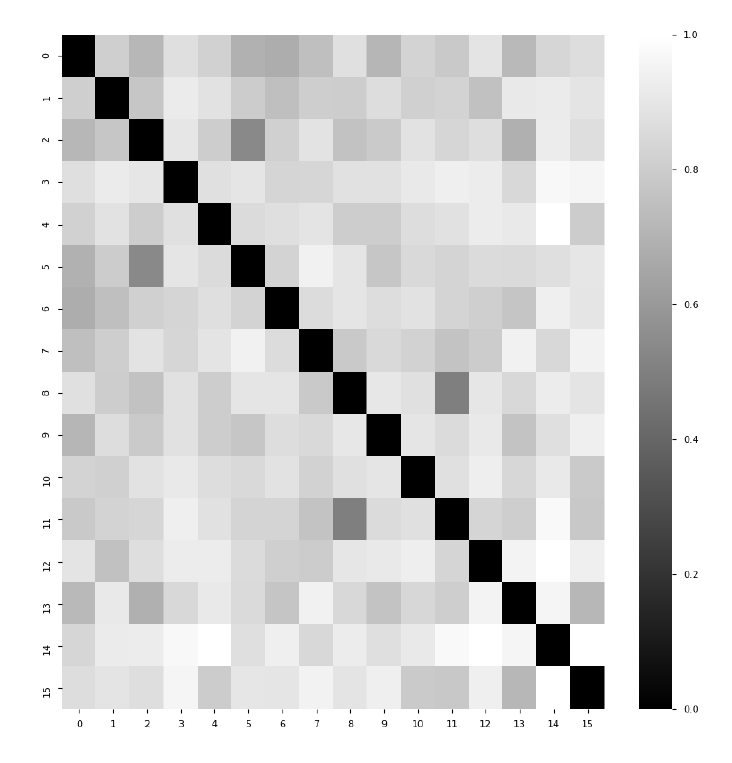
\includegraphics[width=0.8\textwidth]{allo7}
  \label{fig:allo7}
\end{figure}  

Для сравнения полученной кластеризации статей была проведена кластеризация с помощью алгоритма KMeans, показавшая схожие результаты (Рис. \ref{fig:allo8}).

\begin{figure}[H]
  \caption{Сравнение предлагаемого в статье алгоритма кластеризации и алгоритма KMeans.}
  \centering
    \includegraphics[width=0.8\textwidth]{allo8}
  \label{fig:allo8}
\end{figure}  

С помощью KMeans была произведена кластеризация статьей, а затем из графа соавторства были определены кластеры авторов на основании полученных кластеров статей.

\section[Вероятностная модель текста]{Вероятностная модель скрытых тем на основе архива журнала ``Нефтяное Хозяйство''}

Вопрос о том, по какому пути движется прикладная наука и технологии, является ключевым для любой научно-технической области. 
Традиционно определение векторов развития производилось и производится экспертами по предметному направлению, однако значительный рост объемов информации и увеличение числа направлений развития свидетельствуют о необходимости доработки и совершенствования этого инструментария и выработке дополнительных методов исследования индустриальных трендов. 
В данном исследовании автором проанализированы тренды нефтяной индустрии посредством автоматизированной обработки текстов научных статей в отраслевом журнале ``Нефтяное хозяйство''. 
Выявляя наиболее часто встречаемые темы в журнале за период с 2008 по 2016 годы, мы сделали вывод об увеличении значимости трудноизвлекаемых запасов и росте интереса к методам разработки подобных месторождений. 

Журнал ``Нефтяное хозяйство'' посвящен нефтегазовой проблематике.
В нем публикуются статьи, посвященные широкому кругу вопросов нефтегазового сектора: экономических, технических, технологических, экологических и информационных. Издание насчитывает почти вековую историю и выходит каждый месяц с 1920 года. 
Все публикуемые статьи проходят процедуру рецензирования.
Журнал включен в Российский индекс научного цитирования (РИНЦ) и международную систему индексирования Scopus. 
Материалы журнала находятся в закрытом доступе и распространяются по подписке. 
Основные рубрики журнала: 

\begin{itemize}
\tightlist
\item новости нефтегазовых компаний;
\item нефтяная и газовая промышленность;
\item экономика, управление, право;
\item геология и геологоразведочные работы;
\item бурение;
\item разработка и эксплуатация нефтяных месторождений;
\item проектирование и обустройство месторождений;
\item техника и технологии добычи нефти;
\item нефтепромысловое оборудование;
\item транспорт и подготовка нефти;
\item экологическая и промышленная безопасность;
\item информационные технологии. 
\end{itemize}

Как видно, журнал подробно рассматривает практически все аспекты функционирования нефтяных компаний – от экономико-правовых вопросов, до технологических аспектов и тонкостей.

Для проведения исследования редакцией были любезно предоставлены архивы статей журнала ``Нефтяное хозяйство'' за период 2008-2016 гг. 
В выборке содержится 108 выпусков журналов, со статьями от 3517 авторов. 
В каждом из выпусков журналов содержатся все статьи номера, таким образом, была получена сплошная выборка, в которой содержались материалы по самым различным содержательным направлениям. 
В среднем, в номере журнала ``Нефтяного хозяйства'' около 20-25 статей. 
Были рассмотрены именно выпуски журнала, так как они являлись единицей анализа. 
Авторами статей журнала являются научные сотрудники, инженеры и отраслевые эксперты, многие из них кандидаты и доктора наук. 

Процесс исследования имел следующие этапы:

\begin{enumerate}
\item 
Изначально архивы представлены в виде файлов в формате PDF. 
Иногда это был единый файл (биндер) со статьями за весь год, а иногда разрозненные файлы с отдельными статьями. 
В обоих случаях файлы были предназначены для печати, то есть содержали оглавления, номера страниц, тематические вставки и другие редакторские элементы. 
Для анализа нужны были только тексты в виде предложений поэтому автором был реализован программный модуль для приведения всех данных к такому формату. 
Отметим, что, исходя из выбранной методики, важно было сохранить порядок слов и разделение на предложения, при этом необходимо было сохранять принадлежность к выпуску, а не к статье, так как минимальной единицей временного анализа выбран один выпуск.

\item 
На втором этапе анализа происходило приведение слов к основным формам. 
Для анализа и сравнения слов методами частотного и вероятностного анализа необходимо сузить возможные варианты употребления словоформ. 
Существуют несколько алгоритмов для решения этой задачи (нормализации текста), в данном случае был использована стемминг. 
Стеммингом называют процедуру нахождения основы слова, при этом основа и корень слова могут различаться между собой.  
Одним из наиболее распространенных инструментов является стеммер Портера, который, однако, часто обрезает слово больше необходимого, что затрудняет получение правильной основы слова, например, кровать->крова. 
Также стеммер Портера не справляется со всевозможными изменениями корня слова (например, выпадающие и беглые гласные), характерными для русского языка. 
Поэтому автор остановился на использовании технологии стемминга компании ``Яндекс'' - MyStem. 
Данная программа производит морфологический анализ текста на русском языке. 
Она умеет строить гипотетические разборы для слов, не входящих в словарь и предлагает несколько вариантов основ слова. 
Тем не менее, автор сочел необходимым поддерживать обратный словарь для полученных словоформ, чтобы сохранять связь между изначальным словом и полученной словоформой. Отдельной веткой обработки подвергались аббревиатуры, широко распространенные в нефтегазовой отрасли. 
Определение аббревиатур производилось на основе словаря аббревиатур, созданного и поддерживаемого в компании ГазпромНефть в рамках проекта Корпоративной Википедии \cite{khasanov2016corporate}.

\item 
На третьем этапе исследования проводилось формирование словаря. 
Известно, что наибольшую смысловую нагрузку несут не одиночные слова, а сочетания слов, в частности пары слов – биграммы. 
Для выделения биграммов автором был использован эвристические алгоритмы. 
Была составлена матрица биграммов в окрестности 5 слов для каждого из предложений. 
Затем были рассчитаны частоты использования каждого из биграммов, после чего были зафиксированы 5\% наиболее встречаемых словосочетаний.

\item 
На четвертом этапе словари отдельных слов и биграммов были объединены для общей обработки алгоритмами выделения тематик. 
Получившийся словарь был проанализирован, на предмет выделения высоко- и низкочастотных слов для их фильтрации. 
Традиционно окончательное формирование словаря производится с помощью стоп-слов. 
Алгоритмы выделения стоп-слов не использовались автором в данной статье. 
Это решение было обусловлено тем, что добавление словаря стоп-слов не добавляло точности и вносило субъективный характер исследования.

\item 
На заключительном пятом этапе производилось построение модели тематик. 
Для этого был использован инструмент BigARTM \cite{ianina2017multi}. 
На этом этапе были получены матрицы распределение тем для документа ($\Theta$) и распределение слов для темы ($\Phi$). 
Для повышения точности алгоритма автором был применен аналитический подход, уточняющий регуляризационные параметры на основании метрик. 
\end{enumerate}

Основной метрикой для выявления факта сходимости модели тем является метрика Perplexity. 
График зависимости Perplexity от количества проходов по корпусу текстов отображен на (Рис. \ref{fig:nx1}).
\begin{figure}[H]
  \caption{Зависимость метрики Perplexity от количества проходов по корпусу текстов.}
  \centering
    \includegraphics[width=0.8\textwidth]{nx1}
  \label{fig:nx1}
\end{figure}  

Из (Рис. \ref{fig:nx1}) видно, что за три прохода модель показала приемлемую сходимость и не нуждается в дальнейшей оптимизации. 

Важными метриками качества модели тем являются степень разрежённости матриц $\Phi$ и $\Theta$. Повлиять на эти метрики можно с помощью параметров $\tau$, соответствующих регуляризаторов. На рисунках Рис. \ref{fig:nx2}  и Рис. \ref{fig:nx3} отображены зависимости для разрежённости матриц  $\Phi$ и $\Theta$.

\begin{figure}[H]
  \caption{Зависимость разрежённости матрицы $\Theta$ от параметра регуляризации $\tau$.}
  \centering
    \includegraphics[width=0.8\textwidth]{nx2}
  \label{fig:nx2}
\end{figure}  

\begin{figure}[H]
  \caption{Зависимость разрежённости матрицы $\Phi$ от параметра регуляризации $\tau$.}
  \centering
    \includegraphics[width=0.8\textwidth]{nx3}
  \label{fig:nx3}
\end{figure}  

На основании зависимостей отображенных на  Рис. \ref{fig:nx2}  и Рис. \ref{fig:nx3} автором были выбраны параметры регуляризации модели тем, позволяющие достичь оптимального соотношения между значимыми терминами и шумовыми.

Тематическая модель, полученная в результате данного исследования, может быть представлена в различных формах. Уровень шумовых терминов мешает интерпретировать результаты, поэтому от запланированных 12 тем содержательных осталось шесть. В Таблице (Таб. \ref{tab:nx1}) представлены темы выделенные с помощью модели. 

\begin{table}[H]
\centering
\caption{Фрагмент матрицы $\Phi$ для терминов  с максимальными вероятностями.}
\label{tab:nx1}
\resizebox{\textwidth}{!}{%
\begin{tabular}{|l|l|l|l|l|l|}
\hline
\textbf{Тема1} & \textbf{Тема2} & \textbf{Тема3} & \textbf{Тема4} & \textbf{Тема5} & \textbf{Тема6} \\ \hline
электронный & ЭЦН & сдвиг & почва & нефтегазоносность & ингибитор \\ \hline
знание & УЭЦН & сигнал & добавка & свод & разлом \\ \hline
автоматизация & сероводород & окисление & композиция & компания & деформация \\ \hline
интегрировать & фациальный & разрушение & знание & впадина & трещиноватость \\ \hline
пользователь & гамма & деформация & агрегат & сепарация & исследовательский \\ \hline
архив & доломит & реологический & загрязнение & миграция & известняк \\ \hline
хранение & замер & песчаный & ПЗП & прогнозный & порода \\ \hline
доступ & депрессия & осадки & надежность & активность & политехнический \\ \hline
подразделение & агент & капиллярный & камень & филиал & штанга \\ \hline
платформа & каротаж & сечение & окисление & цемент & приемистость \\ \hline
\end{tabular}%
}
\end{table}

Можно с уверенностью сказать, что термины, собранные в столбце $Тема1$ характеризуют тематику управления знаниями. 
В столбце $Тема2$ представлена тема добычи. 
Остальные столбцы тоже могут быть достаточно однозначно проинтерпретированы. 
А для машинной обработки набор терминов важнее чем обобщающая его тема.

\begin{figure}[H]
  \caption{Матрица $\Theta$: Распределение тем для документов.}
  \centering
    \includegraphics[width=0.8\textwidth]{nx4}
  \label{fig:nx4}
\end{figure} 

На Рис. \ref{fig:nx4} представлена матрица $\Theta$, дающая представление как полученные тематики распределены в каждом из анализируемых выпусков. 
Можно увидеть, что тема с $Тема 9$ представлена во всех выпусках – это общая информация, поздравления, реклама. 
Полученное представление так же позволяет выбирать наиболее релевантные выпуски с определенной темой. 

Важно отметить, что выбранный автором метод показал высокую скорость анализа, что делает его возможным для применения в онлайновых процессах поиска. 
Например, на сайте издательства в качестве средства улучшающего поиск и дающего рекомендации читателям по статьям со схожей тематикой. 
Также следует отметить, что данная методика может быть в дальнейшем усовершенствована и адаптирована для анализа существенно больших массивов динамических данных и выделения ключевых направлений технологического развития как в более широких, так и в более узких областях. 

\section[Скрытые направления исследований]{Разведка скрытых направлений научных исследований в нефтегазовой отрасли}

По оценкам автора более 6 тысяч научно-практических статей публикуется ежегодно на основном нефтегазовом портале https://OnePetro.org. Большинство лиц, принимающих решения в нефтяной индустрии желают быть в курсе основных технологических трендов. Но лишь единицы из них имеют время на то, чтобы прочитать одну-две научных статьи в неделю. Драматически важно чтобы это время было использовано с максимальной эффективностью и выбранные научные статьи представляли действительно сфокусированные исследования высокого качества, а не вторичное перемалывание известных фактов. 

Автор выбрал 1696 статей с сайта OnePetro для углубленного анализа. Эти документы были в формате PDF и нуждались в трансформации в формат пригодный для текстового анализа. Автор использовали библиотеку Apache TIKA для конвертации PDF в текст. В процессе трансформации была восстановлена пунктуация. После получения корпуса текстов необходимо было создать словарь для терминов.

На Рисунке \ref{fig:op3_1} изображена гистограмма частот терминов (слов), которые употреблялись в выбранных статьях и доля выбранных терминов для дальнейшего анализа. С помощью такой выборки автор избавилися от слов с низкими и высокими частотами употребления в коллекции текстов.

\begin{figure}[H]
  \caption{Распределение частот терминов в корпусе текстов.}
  \centering
    \includegraphics[width=0.8\textwidth]{op3_fig1rus}
  \label{fig:op3_1}
\end{figure}  

В соответствии с методикой, изложенной в разделе \ref{sec:topicmodel}, в начале автор произвел тренировку PLSA topic model чтобы определить
скорость сходимости по метрике \emph{Perplexity}. Зависимость \emph{Perplexity} от количества проходов отображена на Рисунке \ref{fig:op3_2}.

\begin{figure}[H]
  \caption{Зависимость Perplexity от количества проходов.}
  \centering
    \includegraphics[width=0.8\textwidth]{op3_fig2rus}
  \label{fig:op3_2}
\end{figure}  

Из рисунка \ref{fig:op3_2} видно, что модель хорошо сходится уже на 20 прогонах.

Для дальнейшего обучения к модели были добавлены следующие регуляризаторы:

\begin{enumerate}
\def\labelenumi{\arabic{enumi}.}
\tightlist
\item Sparse Theta -- для увеличения разрежённости матрицы $\Theta$ для основных тематик,
\item Sparse Phi -- для увеличения разрежённости матрицы $\Phi$ для основных тематик,
\item Smooth Theta -- для уплотнения матрицы $\Theta$ для шумовых тематик,
\item Smooth Phi -- для уплотнения матрицы $\Phi$ для шумовых тематик.
\end{enumerate}

Для определения параметров регуляризаторов были проведены следующие пробные эксперименты по обучению модели. 
Результаты этих пробных экспериментов оценивались по метрикам разрежённости матриц $\Phi$ и $\Theta$ . 
Для уплотнения матриц и предполагается использовать полученные параметры $\tau$ с  обратным знаком.

На рисунке \ref{fig:op3_3} приведена зависимость разрежённости матрицы для нескольких значений параметра регуляризации $ \tau $.
\begin{figure}[H]
  \caption{Зависимость разрежённости матрицы $ \Phi $ для нескольких значений параметра регуляризации $ \tau $.}
  \centering
    \includegraphics[width=0.8\textwidth]{op3_fig3rus}
  \label{fig:op3_3}
\end{figure}  

На основании зависимости отображенной на рисунке \ref{fig:op3_3} для дальнейших экспериментов было
выбрано значение $ \tau = -10 $. При таком значении $ \tau $ после 25 прогонов в матрице $\Phi $ остается 92\% нулевых значений.

На рисунке \ref{fig:op3_4}  приведена зависимость разрежённости матрицы $\Theta$  для нескольких значений параметра регуляризации $ \tau $.

\begin{figure}[H]
  \caption{Зависимость разрежённости матрицы $ \Theta $ для нескольких значений параметра регуляризации $ \tau $.}
  \centering
    \includegraphics[width=0.8\textwidth]{op3_fig4rus}
  \label{fig:op3_4}
\end{figure}  

На основании зависимости отображенной на рисунке  \ref{fig:op3_4}  для дальнейших экспериментов было выбрано значение $ \tau  = 10 $. 
При таком значении $ \tau $ после 25 прогонов в матрице остается 78\% нулевых значений.

Для того, чтобы качественно оценить полученную тематическую модель автор применил метод визуальных оценок качества кластеризации.
Рассмотрим темы в тематической модели как кластеры. Тогда хорошо выделенная тема должна описываться ``близкими'' словами и отстоять
``далеко'' от слов, образующих другие темы.

Чтобы сравнивать ``близость'' и ``удаленность'' слова были представлены в виде векторов с помощью алгоритмов FastText и GloVe. Для отображения
полученных векторов были использованы два алгоритма уменьшения размерности: TSNE и MDS.

Алгоритм TSNE имеет несколько значимых параметров, таких как метрика,
perplexity и learning rate. Автор рассмотрел значения perplexity от 5
до 50 с шагом 5 и перебрал следующие метрики расстояний: cosine и euclidean. 
Наиболее наглядные результаты представлены на \ref{fig:op3_5} и \ref{fig:op3_6}. 

\begin{figure}[H]
  \caption{Кластеры слов по тематикам. Векторы слов получены с помощью FastText. Визуализация получена с помощью TSNE с параметрами preplexity=30 и метрикой cosine.}
  \centering
    \includegraphics[width=0.8\textwidth]{op3_fig5rus}
  \label{fig:op3_5}
\end{figure}

\begin{figure}[H]
  \caption{Кластеры слов по тематикам. Векторы слов получены с помощью GloVe. Визуализация получена с помощью TSNE с параметрами preplexity=30 и метрикой cosine.}
  \centering
    \includegraphics[width=0.8\textwidth]{op3_fig6rus}
  \label{fig:op3_6}
\end{figure}

На основе \ref{fig:op3_5} и \ref{fig:op3_6} можно наблюдать группировки слов, образующих тематики. Отметим, что расстояния при трансформации
векторного пространства методом TSNE не сохраняются, но сохраняются пропорции расстояний.

Преобразование векторного пространства с помощью метода MDS отображены  на \ref{fig:op3_7} и \ref{fig:op3_8}.

\begin{figure}[H]
  \caption{Кластеры слов по тематикам. Векторы слов получены с помощью FastText. Визуализация получена с помощью MDS.}
  \centering
    \includegraphics[width=0.8\textwidth]{op3_fig5rus}
  \label{fig:op3_7}
\end{figure}

\begin{figure}[H]
  \caption{Кластеры слов по тематикам. Векторы слов получены с помощью GloVe. Визуализация получена с помощью MDS.}
  \centering
    \includegraphics[width=0.8\textwidth]{op3_fig6rus}
  \label{fig:op3_8}
\end{figure}

На рисунках \ref{fig:op3_7} и \ref{fig:op3_8} можно видеть группировку слов, образующих тематики. 
Алгоритм MDS использует евклидову метрику для вычисления расстояний.

Полученные с помощью MDS и TSNE результаты для FastText и GloVe
показывают наличие кластеров слов , соответствующих тематикам. Так же мы
видим наличие шумовых слов в тематиках.

В таблице \ref{tab:op3_1}  представлены top10 терминов, образующих основные тематики до регуляризации.

\begin{table}[H]
\centering
\caption{Top10 терминов, образующих тематики до регуляризации.}
\label{tab:op3_1}
\resizebox{\textwidth}{!}{%
\begin{tabular}{lllllllll}
Топик & sbj0 & sbj1 & sbj2 & sbj3 & sbj4 & sbj5 & sbj6 & sbj7 \\
Терм1 & liquid & sand & stress & injection & corrosion & casing & injection & safety \\
Терм2 & equation & shale & fractures & history & nace & mud & recovery & management \\
Терм3 & velocity & porosity & hydraulic & matrix & samples & cement & steam & risk \\
Терм4 & pipe & logging & fracturing & optimization & concentration & hole & viscosity & assessment \\
Терм5 & experimental & pore & proppant & recovery & acid & tubing & core & human \\
Терм6 & eq & samples & shale & porosity & treatment & string & heavy & health \\
Терм7 & coefficient & core & stage & linear & steel & drill & injected & company \\
Терм8 & multiphase & log & treatment & matching & ph & bit & polymer & team \\
Терм9 & equations & sample & conductivity & match & inhibitor & completion & flooding & equipment \\
Терм10 & mass & logs & stimulation & cumulative & chemical & mpd & solvent & environmental
\end{tabular}%
}
\end{table}

В таблице \ref{tab:op3_2} представлены top10 терминов, образующих основные тематики после применения обучения с регуляризацией.

\begin{table}[H]
\centering
\caption{Top10 терминов, образующихосновные тематики после применения обучения с регуляризацией.}
\label{tab:op3_2}
\resizebox{\textwidth}{!}{%
\begin{tabular}{lllllllll}
Топик & sbj0 & sbj1 & sbj2 & sbj3 & sbj4 & sbj5 & sbj6 & sbj7 \\
Терм1 & liquid & shale & fracturing & injection & corrosion & casing & recovery & safety \\
Терм2 & pipeline & porosity & proppant & fractures & nace & cement & injection & management \\
Терм3 & pipe & logging & hydraulic & shale & concentration & mud & steam & risk \\
Терм4 & velocity & sand & stress & matrix & samples & hole & core & human \\
Терм5 & multiphase & pore & fractures & hydraulic & inhibitor & mpd & viscosity & health \\
Терм6 & slug & samples & stage & recovery & acid & bit & flooding & business \\
Терм7 & friction & core & shale & fractured & ph & drill & solvent & assessment \\
Терм8 & bhr & spwla & treatment & bakken & steel & string & heavy & training \\
Терм9 & group & clay & conductivity & porosity & houston & pipe & saturation & company \\
Терм10 & holdup & symposium & stages & unconventional & iron & liner & surfactant & activities
\end{tabular}%
}
\end{table}

Из таблиц \ref{tab:op3_1} и \ref{tab:op3_2} мы видим, что основные термины,
формирующие тематики устойчивы к процессам регуляризации. Качество
интерпретируемости тематик улучшается с регуляризацией за счет появления
более конкретных терминов.

Так же представляет интерес поведение тематик для отбора шумовых
терминов. В таблице приведены шумовые тематики до и после регуляризации.

\begin{table}[H]
\centering
\caption{Top10 терминов, образующих шумовые тематики до и послеприменения обучения с регуляризацией.}
\label{tab:op3_3}
\resizebox{\textwidth}{!}{%
\begin{tabular}{|l|l|l|l|}
\hline
\multicolumn{2}{|l|}{\textbf{До регуляризации}} & \multicolumn{2}{l|}{\textbf{После регуляризации}} \\ \hline
\textbf{nz0} & \textbf{nz1} & \textbf{nz0} & \textbf{nz1} \\ \hline
pump & wave & pump & stress \\ \hline
pipeline & seismic & sand & equation \\ \hline
esp & seg & completion & seismic \\ \hline
power & frequency & injection & wave \\ \hline
subsea & velocity & tubing & velocity \\ \hline
operating & waves & equipment & numerical \\ \hline
lift & amplitude & operating & x \\ \hline
equipment & x & downhole & pore \\ \hline
installation & elastic & power & our \\ \hline
liquid & offshore & esp & direction \\ \hline
\end{tabular}%
}
\end{table}

Примечательно, что в шумовые тематики попала тема Сейсмики (nz1).
Согласно мнению эксперта сейсмике относятся слова seismic, wave,
velocity, elastic, seg, frequency и amplitude. Статьи по сейсмике мало
представлены в библиотеке OnePetro и действительно могут быть отнесены к
второстепенным. После обучения с регуляризацией в nz1 добавились
несколько терминов связанных с вычислениями, но тема сейсмики осталась.
В частности, термин offshore ушел в основные тематики. С тематикой nz0
все достаточно однозначно. В нее попали часто употребляемые слова,
которые не являются на самом деле шумом.

Рассмотрим результат отнесения моделью документов к определенным
тематикам. Распределение тематик для каждого документа отражены в матрице
$\Theta$ . Для получения более общего представления о происходящем преобразовании
матрицы авторы представили ее вид до (Рис. \ref{fig:op3_9}) и после (Рис. \ref{fig:op3_10}) регуляризации в
виде 2D-карт.

\begin{figure}[H]
  \caption{Матрица  $ \Theta $ до регуляризации. По оси x отложены номера документов из коллекции.}
  \centering
    \includegraphics[width=0.8\textwidth]{op3_fig9rus}
  \label{fig:op3_9}
\end{figure}

\begin{figure}[H]
  \caption{Матрица $ \Theta $ после регуляризации. По оси x отложены номера документов из коллекции.}
  \centering
    \includegraphics[width=0.8\textwidth]{op3_fig10rus}
  \label{fig:op3_10}
\end{figure}

Как мы видим из рисунков \ref{fig:op3_9} и \ref{fig:op3_10}  матрица $\Theta$ в процессе
регуляризации становится более разряженной на основных тематиках
(sbj0-sbj10) и более плотной на шумовых тематиках (nz0-nz1).

Например, документ № 555 обладает самым большим весом тематики 0.72
(sbj6). Вероятности других основных тематик для этого документа равны
нулю. Таким образом этот документ согласно модели, полностью посвящен
тематике sbj6, представленной словами
(Таб. \ref{tab:op3_2}): recovery, injection, steam,
core, viscosity, flooding, solvent, heavy, saturation, surfactant. При
помощи эксперта sbj6 дано название: ``Chemical enhanced oil recovery''.

Но с другой стороны, мы можем проверить по корпусу текстов нашей
выборки, что данный документ соответствует статье с названием ``Low
Tension Gas Process in High Salinity and Low Permeability Reservoirs''.
Вот фрагмент из публичной аннотации этой статьи с сайта
OnePetro.org\footnote{\textsuperscript{}
  https://www.onepetro.org/conference-paper/SPE-179839-MS}:


\textbf{Abstract}
\textit{Chemical enhanced oil recovery (EOR) in carbonate reservoirs has always been technically and economically challenging. Conventional Alkaline-Surfactant-Polymer (ASP) flooding has limited application in low permeability (2-20 mD) and high salinity formations (~200,000 ppm TDS) with a large concentration of divalent cations. Also  into such low permeability reservoirs can be a significant problem with polymer solutions ($\dots$).}

Как мы видим из этого общедоступного фрагмента статьи тематика
определена с высокой точностью. Но более того, из модели мы знаем, что
эта статья действительно сфокусирована на этой тематике. Приобретя
данную статью можно быть достаточно уверенным, что в ней не будет других
тематик.

Важно так же отметить, что можно было и не прибегать к помощи эксперта
для определения названия тематики sbj6, а воспользоваться тем, что
данный документ представлен единственной тематикой и взять название из аннотации статьи.

\section[Глубокий анализ текстов публикаций]{Выявление негативных отзывов о технологиях в текстах}
\label{seq:emo}
Использование искусственных нейронных сетей для анализа текстов получило развитие в середине 90-х годов в работах \cite{ng1997feature,lam1999feature,lam1999automatic}. 

Но из-за высоких требований к вычислительным ресурсам для обучения нейронных сетей оставалось академической дисциплиной.
Ускорение исследований в этом направление связано с ростом скорости вычислений и с появлением таких новых архитектур искусственных нейронных сетей как сверточные нейронные сети \cite{kim2014convolutional} и рекуррентные нейронные сети \cite{mikolov2010recurrent}.
Для обучения нейронных сетей всегда были нужны значительные массивы размеченных данных.
А с появлением большего количества слоев с нейронами потребность в размеченных данных выросла в разы. 
Для примера, чтобы обучить искусственную нейронную сеть со ста тысячью коэффициентами нужны десятки тысяч размеченных текстов. 
А для архитектуры глубоких нейронных сетей количество обучаемых коэффициентов составляет миллионы \cite{krizhevsky2012imagenet,miller1995wordnet}.
Поэтому обучение искусственной нейронной сети на собственных данных означает выделение определенного времени и ресурсов на разметку. 
Другими словами, каждый классифицируемый объект человек должен отнести к одному из классов «вручную».
Не так давно появились размеченные корпусы текстов с открытым доступом, например,
UMICH SI650 \footnote{https://www.kaggle.com/c/si650winter11} , TreeBank \footnote{http://nlp.stanford.edu/sentiment/treebank.html}, 
Twitter Sentiments \footnote{http://www.sananalytics.com/lab/twitter-sentiment/} , MPQA Opinion Corpus \cite{http://mpqa.cs.pitt.edu} и работы по их анализу \cite{maas2011learning,socher2013recursive, akkaya2009subjectivity}.

Для данного эксперимента автор применил методику Transfer learning.
В качестве размеченного набора данных автором были выбраны отзывы о кинофильмах \cite{maas2011learning}. 
В этом наборе данных содержится 25 тысяч положительных и 25 тысяч отрицательных отзывов. 
Набор данных таким образом сбалансирован для обучения и валидации модели классификации.
Длинна отзывов варьируется от 5 до 977 слов и отображена на рисунке (Рис. \ref{fig:op4_2}).
\begin{figure}[ht]
	\centering
	\includegraphics[width=0.8\textwidth]{op4_2}
	\caption{Распределение длин отзывов.}
	\label{fig:op4_2}
\end{figure}

При составлении словаря по отзывам были отброшены низкочастотные слова, то есть слова, встречающиеся в документах редко. Распределение частот слов по документам отображено на диаграмме (Рис. \ref{fig:op4_3} ).
\begin{figure}[ht]
  \centering
  \includegraphics[width=0.8\textwidth]{op4_3}
  \caption{Распределение частот слов по документам.}
  \label{fig:op4_3}
\end{figure}

В качестве набора данных для тестирования были выбраны 1696 научно-практических статей с портала OnePetro.org.  

Для построения векторной модели текста была использована обученная модель GloVe. 
Были использованы вектора с размерностью 100 и 300. 
Преимущества от использования обученной векторной модели текста состоит в существенном сокращении объема вычислений.
Количество обучаемых параметров для создания векторной модели текста в разы превосходит количество параметров для выбранных автором архитектур моделей классификации. 

Автор ограничил себя классом моделей, построенных на основе искусственных нейронных сетей. 
Среди архитектур искусственных нейронных сетей используемых для классификации текстов можно выделить CNN-LSTM и Stacked LSTM.  
Автором были выбраны следующие три варианта архитектур моделей для классификации с использованием искусственных нейронных сетей.

\begin{enumerate}
\tightlist
\item Рекуррентная нейронная сеть из одного слоя LSTM.  Далее будем называть эту архитектуру RNN и отдельно указывать количество элементов в LSTM слое.
\item Сверточная нейронная сеть из одного слоя Dropout-Conv1D-Conv1D-MaxPooling и рекуррентная нейронная сеть из одного слоя элементов LSTM. Далее будем называть эту архитектуру CNN-LSTM и отдельно указывать количество элементов и параметры сверточных слоев.
\item Рекуррентная нейронная сеть из двух слоев LSTM. Далее будем называть эту архитектуру RNN-2 и отдельно указывать количество элементов в LSTM слое.
\end{enumerate}

Для рассматриваемых архитектур моделей классификации автор выбрал следующие существенные гиперпараметры:
\begin{itemize}
\tightlist
\item Тип модели классификации: RNN, CNN-LSTM, RNN-2.
\item Размерность словаря. В зависимости от фильтров низкочастотных слов размерность словаря изменялась от 2000 до 200000 слов.
\item Размерность векторной модели текста: 100 и 300
\item Длинна фрагмента текста: 80, 128 и 196.
\end{itemize}

Обучение моделей классификации производилось параллельно на нескольких серверах. 
Набор данных содержал равное количество положительный и отрицательных отзывов поэтому для оценки качества обучения была выбрана метрика Accuracy. 
Оптимизация параметров модели для классификации производилась на основании функции перекрестной энтропии (Cross Entropy). 
Для ускорения обучения автором был применен метод ранней остановки обучения на основании метрики Accuracy по валидационному набору данных. Кривые обучения для модели классификации типа RNN отображены на рисунках (Рис. \ref{fig:op4_4} , Рис. \ref{fig:op4_5} ).

\begin{figure}[ht]
  \centering
  \includegraphics[width=0.8\textwidth]{op4_4}
  \caption{Кривая обучения метрики Accuracy для модели классификации типа RNN.}
  \label{fig:op4_4}
\end{figure}

Из зависимости метрики Accuracy для тренировочного и валидационного набора данных (Рис. \ref{fig:op4_4} ) видно, что в районе 42-й итерации обучения метрика Accuracy перестает увеличиваться для валидационного набора данных. 
Это явление означает, что модель начинает переучиваться по метрике Accuracy и обучение следует остановить. 
Данная архитектура модели для классификации не позволяет повышать точность на этом наборе данных.  

\begin{figure}[H]
  \caption{Кривая функции потерь для модели классификации типа RNN.}
  \centering
    \includegraphics[width=0.8\textwidth]{op4_5}
  \label{fig:op4_5}
\end{figure}

Отметим что из зависимости, отображенной на Рис. \ref{fig:op4_5} видно, что значение перекрестной энтропии на валидационном наборе данных начинает не убывать в районе 37 итерации. 
То есть, немногим раньше, чем начинает деградировать метрика Accuracy. 

На основании изложенных выше методик было проведено обучение моделей классификации с различными архитектурами и гиперпараметрами. 
Результаты обучения приведены в таблице (Таб. \ref{tab:op4_1}).

\begin{table}[H]
\centering
\caption{Результаты обучения моделей классификации с различными гиперпараметрами.}
\label{tab:op4_1}
\resizebox{\textwidth}{!}{%
\begin{tabular}{|l|l|l|l|l|l|}
\hline
\textbf{Архитектура модели} & \textbf{Количество параметров,  тыс.} & \textbf{Длинна фрагмента текста} & \textbf{Размерность векторного пространства текста} & \textbf{Словарь, количество слов} & \textbf{Точность валидации} \\ \hline
CNN+RNN & 63 & 128 & 100 & 2 300 & 0,85 \\ \hline
CNN+RNN & 63 & 196 & 100 & 2 300 & 0,87 \\ \hline
CNN+RNN & 63 & 196 & 100 & 23 400 & 0,86 \\ \hline
RNN & 69 & 128 & 100 & 2 300 & 0,87 \\ \hline
RNN & 722 & 196 & 300 & 23 400 & 0,88 \\ \hline
RNN & 81 & 128 & 100 & 47 969 & 0,85 \\ \hline
RNN-2 & 161 & 128 & 100 & 2 300 & 0,86 \\ \hline
RNN-2 & 161 & 196 & 100 & 2 300 & 0,87 \\ \hline
RNN-2 & 1 443 & 196 & 300 & 23 000 & 0,87 \\ \hline
RNN-2 & 1 443 & 196 & 300 & 248 739 & 0,85 \\ \hline
RNN-2 & 1 443 & 80 & 300 & 248 739 & 0,85 \\ \hline
\end{tabular}%
}
\end{table}

Лучшее значение метрики Accuracy на валидационном наборе данных показала модель RNN со словарем из 23 тысяч слов и размерностью векторной модели текста равной 300. Отметим, что на тестовом наборе данных значение метрики Accuracy для данной модели составило 88\%.

Полученная модель была использована для предсказания тональности научных статей портала OnePetro.org.  Каждая научная статья разбивалась на фрагменты длинной 196 слов для оценки эмоциональной окраски. Затем фрагменты статей собирались обратно для получения эмоциональной карты всей статьи. Таким образом, можно было определить фрагменты статьи, обладающие аномальными эмоциональными окрасками, такими как разочарование и удовлетворенность. 

Данное исследование не принимает в расчет семантику текста, поэтому предмет эмоциональной окраски автоматически не определялся. Выбранные фрагменты статьи необходимо проанализировать с помощью эксперта. Но такой подход к аннотированию статьи позволил найти сложно обнаруживаемые фрагменты. В Таблице \ref{tab:op4_2} приведены примеры эмоциональных фрагментов статей.

\begin{table}[H]
\centering
\caption{Выявленные эмоциональные фрагменты статей.}
\label{tab:op4_2}
\resizebox{\textwidth}{!}{%
\begin{tabular}{|l|}
\hline
\textit{the results from pilot tests which were using as injectant are disappointing and the results from pilot tests which were using natural gases are encouraging} \\ \hline
\textit{to sum up diffusion mechanism for in pilot tests had not been well recognized which in turn did not enhance oil production rate in those wells} \\ \hline
\textit{the outstanding result from this study} \\ \hline
\textit{using the other forward model result  dramatically bad} \\ \hline
\end{tabular}%
}
\end{table}

Так же автор разработал цветовое представление эмоциональной окраски статей в зависимости от вероятности отнесения фрагмента текста к положительной или отрицательной эмоциональной окраске.

\begin{figure}[H]
  \caption{Карта полярности эмоциональной окраски статей 1696 статей. По оси x отложен порядковый номер статьи, по оси y эмоциональная окраска фрагментов статьи. На цветовой шкале отображена цифровая характеристика эмоциональности: негативная (-1), позитивная (+1).}
  \centering
    \includegraphics[width=0.8\textwidth]{op4_6}
  \label{fig:op4_6}
\end{figure}

На рисунке (Рис. \ref{fig:op4_6}) эмоциональность фрагментов статей отображена в виде карты. Для каждой статьи на оси X цветом отображена эмоциональность каждого фрагмента последовательно по оси Y. 

Научные статьи используют академическую лексику и ожидать в них градус эмоций сравнимый с отзывами на кинофильмы было бы наивно. Но современные концепции обработки текста, основанные на анализе контекста, позволяют выделять и классифицировать изменения эмоциональности достаточно точно для того, чтобы обрабатывать даже научные статьи. Автор считает, что проведенное исследование открывает возможности по созданию дополнительных инструментов для аннотации и классификации научных текстов.


\chapter{Выводы}
\label{conclusions}

В последние годы вопрос о том, по какой траектории происходит развитие нефтегазового комплекса, как и всей энергетической системы, приобретает все больший интерес, как со стороны экспертов, так и со стороны широкой общественности \cite{bakhtin2017trend,kuzminov2017global}. 
Этому способствует несколько факторов. 


\begin{itemize}
\tightlist
\item Во-первых, темпы экономического развития приводят к значительному росту мирового энергопотребления. Как отмечается в докладе Аналитического Центра при Правительстве РФ , значительный рост потребления энергоресурсов происходит за счёт развивающихся стран, преимущественно Азиатско-тихоокеанского региона, в то время как в развитых странах объем выработки электроэнергии стабилен, а динамика потребления схожа с тенденциями общеэкономических приростов и спадов. 

\item Во-вторых, наблюдается изменение структуры запасов углеводородов. Как отмечается в «Энергетической стратегии России на период до 2035 года»  (сформулированной в 2015 году), отечественная нефтяная отрасль сталкивается с такой проблемой, как «увеличение себестоимости добычи вследствие преобладания труднодоступных запасов нефти (далее по тексту ТРиЗ) и большой выработанности действующих месторождений, что усложняет удержание достигнутых уровней добычи нефти». При этом одной из задач, ставящейся перед нефтяным сектором, является освоение ТРиЗ в объёмах до 17\% от общей добычи, которая может быть решена путём развития добывающих технологий. 

\item Наконец, в-третьих, всё большую роль в энергетическом секторе играют источники возобновляемой энергии (т.н. ВИЭ), что сказывается на структуре энергетических рынков . Эксперты, политики и граждане всё больше озабочены экологическими и климатическими вызовами, что свидетельствует о необходимости диверсификации энергоносителей. Дополнительно стоит отметить негативное влияние внешних экономических и политических ограничений на сырьевой сектор российской экономики.
\end{itemize}

Таким образом, энергетическая сфера находится в процессе постоянной трансформации, а одним из важных вопросов повестки дня нефтяного сообщества является оптимизация методов геологоразведки, добычи и использования энергоносителей. 

Анализировать, по какой траектории движется изменение научно-технических и технологических процессов нефтедобычи, можно несколькими способами. Наиболее очевидным видится опрос экспертов, специализирующихся на вопросах добычи. 

Методы экспертных опросов (также называемые методами экспертных оценок) широко используются в различных исследованиях, в которых невозможны или труднодоступны другие формы исследований ввиду отсутствия объективных данных. Таким образом реализуется подавляющее большинство форсайт-исследований. К достоинствам экспертного опроса можно отнести их относительную простоту и доступность, а также возможность применения в случае отсутствия информации об изучаемом явлении. 

В то же время очевидным недостатком экспертного опроса являются возможный субъективизм и ограниченность экспертов, их приверженность определенной точке зрения. Как отмечается в работе Бахтина с соавторами \cite{bakhtin2017trend}, в течение последних лет объёмы экспертно-аналитической и научной литературы, а также информации в целом, стремительно растут (по некоторым оценкам объёмы информации удваиваются каждые два года), так что задача получения, фильтрации, переработки и рефлексивного восприятия всей информации становится фактически невозможной. При этом эксперту необходимо развиваться и совершенствоваться в различных содержательных направлениях, что требует ещё больших трудовых и временных инвестиций. Это свидетельствует о необходимости разработки и формирования дополнительной обратной связи, которая призвана помочь экспертному и профессиональному сообществу анализировать огромные объемы информации и выделять из нее наиболее релевантные аспекты, в частности – выявлять технологические тренды. 

С развитием автоматизированных методов обработки неструктурированных данных, в частности текстовых данных, популярность набирает тематическое моделирование научных текстов \cite{blei2006dynamic}. Как было продемонстрировано в работе Блея и Лафферти, тематическое моделирование оказывается перспективным инструментов отслеживания трендов в таких научных направлениях, как ядерная физика и нейронауки \cite{Blei:2003}, технологии агропромышленного комплекса \cite{bakhtin2017trend} и так далее. Изучение автоматически выделенных тематик во временной перспективе иллюстрирует изменение интереса научного сообщества к различным объектам и предметам исследования. Достоинством этого метода является возможность автоматизированной обработки огромных массивов информации и выявления латентных (скрытых) тематик текстов. 
При этом тематическое моделирование нельзя назвать исключительно автоматизированным методом, так как полученные в результате машинной классификации тематики в дальнейшем должны быть вручную просмотрены и проработаны экспертами-специалистами предметной области. Таким образом, тематическое моделирование может рассматриваться как метод, заключающий в себе достоинства и автоматизированной обработки текста, и экспертной оценки. Реализация подобного метода в приложении к различным содержательным задачам позволит сформировать диалог между наукой и стратегией на принципиально новом уровне.
% 
Тематическое моделирование позволяет оперативно обрабатывать значительные объемы текстов для сужения найденных понятий до небольших значимых фрагментов текста - топиков. Каждый топик
представляется набором слов и от качества этого представления зависит возможная интерпретация.

Автор показал результативность подхода к улучшению интерпретируемости тематик на основе последовательной регуляризации. 

Примененные методы управление отношением «плотность-разрежённость» открывают возможности настройки модели на предметную область текстов. Автор показал принципы создания и настройки модели тематик, которые позволяют вести интеллектуальный поиск (разведку) высоко сфокусированныхисточников знаний.

Кластеризация топиков была проверена с помощью двух методов для векторизации слов (FastText, GloVe) и двух методов для уменьшения размерности векторного пространства (TSNE, MDS). Результаты представлены в виде диаграмм и уверено показывают наличие кластеров.

Подход к анализу текстовой информации на основе моделирования тематик широко используется во внутренних процессах компании ООО «Газпромнефть НТЦ» для оптимизации процессов управления знаниями, выявления наиболее перспективных направлений исследований и поиска opinion leaders в определенных научных направлениях.

Важно отметить, что выбранный автором метод показал высокую скорость анализа, что делает его возможным для применения в онлайновых процессах поиска. Например, на сайте издательства в качестве средства улучшающего поиск и дающего рекомендации читателям по статьям со схожей тематикой. 

Также следует отметить, что разработанная методика может быть в дальнейшем усовершенствована и адаптирована для анализа существенно больших массивов динамических данных и выделения ключевых направлений технологического развития как в более широких, так и в более узких областях. 

Cуществующие прогнозы научно-технического развития (с том числе форсайт-прогнозы) в большинстве своем экстраполируют существующие тренды на долгосрочную перспективу. Таким образом, большой интерес приобретают работы, в которых становится возможным выявление новых технологических направлений, способных существенно видоизменить структуру рынков.

Сами по себе отдельные технологии не следует рассматривать как оторванные и изолированные друг от друга инициативы. В действительности многие технологические направления развиваются параллельно, что является результатом венчурной политики, технологического развития и других сопутствующих факторов. 

Ввиду этого важным направлениям анализа технологических трендов выглядит изучение коэволюции развития сразу нескольких технологий. Именно изучение совокупности научно-технических инициатив позволит содержательно проанализировать направление технологического развития.

%%%

В раделе \ref{sec:di} автором представлен новый взгляд на процесс публикации научных статей. Определены показатели продуктивности и стратегии управления продуктивностью процесса публикаций.
 
Организационная среда должна служить инструментом для повышения эффективности основных производственных процессов. Признание научно-исследовательской организацией того факта, что публикация научных статей является одним из основных производственных процессов означает, что необходимо создавать специальные подразделения, нацеленные на поддержку эффективности этого процесса. Мерой зрелости процесса служит степень разделения труда его участников. Учёный должен заниматься своими прямыми обязанностями - исследованиями и не обязан вникать в детали процессов оформления командировок, эргономичности презентаций и тонкостей общения с издателями и т.п.

Автором разработана ролевая модель, которая позволит разгрузить учёных от формальных трудозатрат по публикации результатов исследований и в некоторых случаях избежать появления «гостевых» соавторов.

Из-за ограничения по объёму публикаций в выпуске издателя организациям необходимо расширять список издательств, в которых публикуются их исследователи, чтобы поддерживать темп роста количества опубликованных статей. 

Показатель продуктивности выражающий долю отвергнутых издательством статей является важной характеристикой процесса публикации результатов исследований не только на организационном, но и на отраслевом уровне. Возможность анализа этого показателя позволяет оценить достаточность ёмкости рынка научных издательств и степень конкуренции за публикацию в изданиях с высоким импакт-фактором. 

%%

В разделе \ref{sec:scrum} автором обобщена и проработана формализация процесса самоорганизации команд для достижения определённой цели -- написания научных статей. 
В исследовании разработан детальный алгоритм образования графа соавторств широко используемого в различных исследованиях.
Сформулированы основные теоретические утверждения, даны определения \emph{укомплектованности команды} и \emph{несостоявшейся научной статьи}. 
Сформулирована гипотеза (Гипотеза \ref{hyp:ex1}) об инвариантность графа соавторства относительно введения Scrum ролей в процесс написания статей.
В результате проведённого автором оптимизационного эксперимента найдены оптимальные значения параметров для построенной  модели написания статей. 
По результатам, сделанным на оптимизированной модели соавторства разработанной автором, эффект от введения гибких методик (Scrum) в процесс написания научных статей небольшими командами соавторов состоит в следующем:

\begin{itemize}
\tightlist
\item  Среднее время написания научной статьи ($T_{pub}$) не  изменяется
\item  Средняя доля несостоявшихся научных статьей   ($Frac_{notpub}$) уменьшается
\end{itemize}

Общее влияние Scrum на процесс написания научных статей командой соавторов является положительным. 
То, что $T_{pub}$ не изменяется может служить экспериментальным подтверждением Гипотезы \ref{hyp:ex1}.

Продуктивность команд, образованных по комплементарному принципу, становится выше от применения гибких методик и Scrum, в частности.

%%%

В эксперименте описанном в разделе \ref{seq:emo} подтверждена гипотеза о возможности выделения эмоционально-окрашенных фрагментов текста из научных статей. Научные статьи используют академическую лексику и ожидать в них градус эмоций сравнимый с отзывами на кинофильмы было бы наивно. Но современные концепции обработки текста, основанные на анализе контексте, позволяют выделять и классифицировать изменения эмоциональности достаточно точно для того, чтобы обрабатывать даже научные статьи. Автор считает, что проведённое исследование открывает возможности по созданию дополнительных инструментов для аннотации и классификации научных текстов. 

Наилучшее оценку по качеству выделения эмоционально окрашенных фрагментов текста показали рекуррентные нейронные сети. Точность по метрике Accuracy для них составила 88\%. Важно отметить, что по скорости обучения рекуррентные сети существенно проигрывают свёрточным сетям. Автор видит объяснение разности в производительности в том, что для обучения сверточных нейронных сетей возможна более высокая степень параллельных вычислений. Тогда как для рекуррентных нейронных сетей необходимо поддерживать последовательность предыдущих состояний нейронов. 

В дальнейших исследованиях автор планирует исследовать применимость эмоционально окрашенных фрагментов текста для задач классификации текстов в качестве признаков. Так же на взгляд авторов, научный интерес представляет анализ синтаксиса эмоционально окрашенных фрагментов текста.

%%%%

В эксперименте описанном в разделе \ref{sec:allo} проведён анализ динамики графа соавторства для одной организации на основании публичных данных о публикациях. Основным аналитическим инструментом был выбран двудольный граф соавторства, методически обоснованный автором в разделе \ref{sec:coath}. 

В работе применён много компонентный подход к прогнозированию изменению свойств графа соавторства. Анализ малых связанных компонент позволил выявить их долю в ежегодном увеличении количества авторов. Отметим, что доля малых компонент в рассматриваемом графе соавторства уменьшается со временем, что является структурным ограничением роста рассматриваемой организации.  

В 2016 году обнаружен «Эффект локтя» - резкое усложнение характера роста графа соавторства по годам.  
Автором сделан прямой прогноз роста на основании тренда роста авторов по годам и уточненный прогноз роста графа соавторства на основе моделирования с помощью методов машинного обучения. 

Проведённое сравнение точности классификаторов определило классификатор на основе нейронной сети как наиболее точный для данной задачи. 

Прогноз, сделанный на основе модели, показал результат (467) существенно меньший чем результат на основе тренда (585). 

В результате проведённого исследования автор сделал вывод о наличии в структуре графа соавторств важной информации о развитии графа соавторств, которая определяет прогноз роста. Что позволяет определить значимые признаки образования новых коллабораций, а также регрессионного предсказания новых связей между уже сформировавшимися исследовательскими коллективами. 

Использование методов векторизации графовых моделей в комбинации с извлечением признаков позволит улучшить точность предсказания появления новых связей, а также качественно измерить публикационную активность на основе публично доступных метрик журналов и конференций .

Так же автором предложен метод выделения направлений научных исследований на основе графа соавторства. Содержательно предложенный метод относится к top-down алгоритмам кластеризации. В качестве критерия выделения кластеров выбрана метрика \textit{Betweenness centrality}. 

В качестве критерия проверки качества кластеров выбрана метрика близости членов кластера и метрика удалённости различных кластеров на основе тематик научных статей, входящих в граф соавторства. 

Результатом применения предложенного метода является укрупненное виденье научных направления развития организации, сделанное на основе публичных данных о публикационной активности сотрудников.

Разработанный автором метод выделения направлений научных исследований на основе графа соавторства опробован на Научно-техническом центра ГазпромНефть. В результате выделены 16 кластеров, характеризующих деятельность организации.
Важными особенностями разработанного метода выделения направлений научных исследований на основе графа соавторства являются следующие:

\begin{itemize}
\tightlist
\item Рекурсивность алгоритма позволяет работать с графами различных порядков.
\item «Жадный» алгоритм определения качества кластеров позволяет корректировать оптимизацию на каждом шаге.
\item Применение двудольного построения графа соавторства позволяет анализировать различные проекции.
\item Работа на основании публичных данных даёт широкие возможности для применения в бизнес разведке.
\end{itemize}

Новизна предложенного автором метода выделения направлений научных исследований на основе графа соавторства состоит в использовании двудольного построения графа соавторства и в динамической модели кластеризации, использующей структурные метрики графа соавторства и метрики близости текстов научных статей.

%%%

Автор создал действующие модели движения персонала в организации и модель выполнения заданий. На основе взаимодействия этих моделей автор построил модель продуктивности, которая, отражает для научно-исследовательской организации изменения ИК. Экспериментальные результаты представлены в разделе \ref{sec:ic}.
 
Согласно мнению многих исследователей ИК сложно измерить. Предложенный автором драйвер ИК в виде производительности научно-исследовательской организации имеет самостоятельную ценность и характеризует ИК, как комплексный показатель организации.  

Автор построил зависимости ИК от различных времён адаптации новичков и различной сложности поступающих заданий, показали асимптотическое поведение ИК. Что позволяет моделировать ситуации разных видов задач, особенностей организации (текучесть, скорость адаптации, сложность задач и пр). 

В исследовании проанализировано как на ИК влияет нагрузка на персонал. Показано как со временем уменьшается продуктивность при высоких нагрузках и необходимости работать дольше 40 часов в неделю. Автором смоделирован эффекты «выгорания» и «усталости» персонала от длительной высокой нагрузки.

Результаты, полученные в исследовании, обладают научной новизной и практической ценностью, дают возможность детального исследования и моделирования динамики продуктивности.

%%%
Созданная автором и описанная в разделе \ref{sec:so} частная модель $\mathbb{M}_{GPN}$ организации оправдала себя как метод исследования социальных явлений и процессов организации посредством их воспроизведения в менее сложных формах и проведения необходимых операций с полученными таким образом аналогами реальных процессов в организационной среде.

Формальная математическая модель $\mathbb{M}_{\Omega}$ организации дает ответы на вопросы о ключевых компонентах деятельности по написанию и публикации научных статей.

Выбранный автором метод создания частной модели $\mathbb{M}_{GPN}$ показал результаты согласующиеся с эмпирическим исследованием публикаций конкретной научно-исследовательской организации.

Был проведен эксперимент по многоагентному симулированию, в котором в качестве агентов выступали научные сотрудники лабораторий, взаимодействующие друг с другом и производящие в качестве результата своей работы научные статьи. Создана частная модель $\mathbb{M}_{GPN}$ путем калибровки на данных НТЦ «Газпромнефть». В работе использовано программное обеспечение Anylogic.

На основании созданной частной модели  автор пришел к необходимости дальнейшего изучения чувствительности от следующих свободных параметров:
\begin{enumerate}
\tightlist
\item Максимальное количество соавторов
\item Среднее количество соавторов в статьях
\item Распределение количества соавторов
\item Количество статей в год на одного сотрудника
\end{enumerate}

Полученные в результате симуляционного эксперимента результаты согласуются с эмпирическими наблюдениями. 
Исходя из этого, автором сделан  вывод о том, что работа исследователей может быть смоделирована с использованием агентного подхода. 
Решение подобной задачи является важным шагом на пути к идентификации механизмов коллективной работы и формирования коллективного наукоемкого продукта.


\listoffigures

\part*{Публикации автора}

\begin{refsection}[authorpapersVAK]
	\nocite{*}
	\printbibliography[title={Публикации в изданиях рекомендованных ВАК.}]
\end{refsection}

\begin{refsection}[authorsvid]
	\nocite{*}
	\printbibliography[title={Свидетельства.}]
\end{refsection}

\begin{refsection}[authorconferences]
	\nocite{*}
	\printbibliography[title={Материалы конференций.}]
\end{refsection}

\begin{refsection}[authorpapers]
	\nocite{*}
	\printbibliography[title={Другие публикации автора.}]
\end{refsection}

\section*{ОСНОВНЫЕ ПОЛОЖЕНИЯ ДИССЕРТАЦИИ ИЗЛОЖЕНЫ В СЛЕДУЮЩИХ РАБОТАХ}

\begin{refsection}[vak]
    \nocite{*}
	\printbibliography[title={Публикации в изданиях, рекомендованных ВАК}]
\end{refsection}

\begin{refsection}[svid]
    \nocite{*}
	\printbibliography[title={Патенты и регистрации программных продуктов}]
\end{refsection}

\begin{refsection}[conf]
    \nocite{*}
	\printbibliography[title={Материалы докладов конференций}]
\end{refsection}

\begin{refsection}[papers]
    \nocite{*}
	\printbibliography[title={Статьи в журналах}]
\end{refsection}



%%% Выходные сведения типографии
\newpage\thispagestyle{empty}

\vspace*{0pt plus1fill}

\small
\begin{center}
    \textit{Краснов Федор Владимирович}
    \par\medskip
    
    Методология измерения эффективности научно-технического центра
    
    \par\medskip
    
    Автореф. дис. на соискание ученой степени доктора технических наук
    \par\bigskip
    
    Подписано в печать XX.XX.XXXX.
    Заказ № XXXXXXXX
    
    Формат 60\(\times\)90/16. Усл. печ. л. 1. Тираж 100 экз.
    %Это не совсем формат А5, но наиболее близкий, подробнее: http://ru.wikipedia.org/w/index.php?oldid=78976454
    
    Типография \blank[0.5\linewidth]
\end{center}
\cleardoublepage

\end{document}



